\documentclass[twoside]{book}

% Packages required by doxygen
\usepackage{calc}
\usepackage{doxygen}
\usepackage{graphicx}
\usepackage[utf8]{inputenc}
\usepackage{makeidx}
\usepackage{multicol}
\usepackage{multirow}
\usepackage{textcomp}
\usepackage[table]{xcolor}

% Font selection
\usepackage[T1]{fontenc}
\usepackage{mathptmx}
\usepackage[scaled=.90]{helvet}
\usepackage{courier}
\usepackage{amssymb}
\usepackage{sectsty}
\renewcommand{\familydefault}{\sfdefault}
\allsectionsfont{%
  \fontseries{bc}\selectfont%
  \color{darkgray}%
}
\renewcommand{\DoxyLabelFont}{%
  \fontseries{bc}\selectfont%
  \color{darkgray}%
}

% Page & text layout
\usepackage{geometry}
\geometry{%
  a4paper,%
  top=2.5cm,%
  bottom=2.5cm,%
  left=2.5cm,%
  right=2.5cm%
}
\tolerance=750
\hfuzz=15pt
\hbadness=750
\setlength{\emergencystretch}{15pt}
\setlength{\parindent}{0cm}
\setlength{\parskip}{0.2cm}
\makeatletter
\renewcommand{\paragraph}{%
  \@startsection{paragraph}{4}{0ex}{-1.0ex}{1.0ex}{%
    \normalfont\normalsize\bfseries\SS@parafont%
  }%
}
\renewcommand{\subparagraph}{%
  \@startsection{subparagraph}{5}{0ex}{-1.0ex}{1.0ex}{%
    \normalfont\normalsize\bfseries\SS@subparafont%
  }%
}
\makeatother

% Headers & footers
\usepackage{fancyhdr}
\pagestyle{fancyplain}
\fancyhead[LE]{\fancyplain{}{\bfseries\thepage}}
\fancyhead[CE]{\fancyplain{}{}}
\fancyhead[RE]{\fancyplain{}{\bfseries\leftmark}}
\fancyhead[LO]{\fancyplain{}{\bfseries\rightmark}}
\fancyhead[CO]{\fancyplain{}{}}
\fancyhead[RO]{\fancyplain{}{\bfseries\thepage}}
\fancyfoot[LE]{\fancyplain{}{}}
\fancyfoot[CE]{\fancyplain{}{}}
\fancyfoot[RE]{\fancyplain{}{\bfseries\scriptsize Generated on Wed Nov 13 2013 01:49:56 for My Project by Doxygen }}
\fancyfoot[LO]{\fancyplain{}{\bfseries\scriptsize Generated on Wed Nov 13 2013 01:49:56 for My Project by Doxygen }}
\fancyfoot[CO]{\fancyplain{}{}}
\fancyfoot[RO]{\fancyplain{}{}}
\renewcommand{\footrulewidth}{0.4pt}
\renewcommand{\chaptermark}[1]{%
  \markboth{#1}{}%
}
\renewcommand{\sectionmark}[1]{%
  \markright{\thesection\ #1}%
}

% Indices & bibliography
\usepackage{natbib}
\usepackage[titles]{tocloft}
\setcounter{tocdepth}{3}
\setcounter{secnumdepth}{5}
\makeindex

% Hyperlinks (required, but should be loaded last)
\usepackage{ifpdf}
\ifpdf
  \usepackage[pdftex,pagebackref=true]{hyperref}
\else
  \usepackage[ps2pdf,pagebackref=true]{hyperref}
\fi
\hypersetup{%
  colorlinks=true,%
  linkcolor=blue,%
  citecolor=blue,%
  unicode%
}

% Custom commands
\newcommand{\clearemptydoublepage}{%
  \newpage{\pagestyle{empty}\cleardoublepage}%
}


%===== C O N T E N T S =====

\begin{document}

% Titlepage & ToC
\hypersetup{pageanchor=false}
\pagenumbering{roman}
\begin{titlepage}
\vspace*{7cm}
\begin{center}%
{\Large My Project }\\
\vspace*{1cm}
{\large Generated by Doxygen 1.8.4}\\
\vspace*{0.5cm}
{\small Wed Nov 13 2013 01:49:56}\\
\end{center}
\end{titlepage}
\clearemptydoublepage
\tableofcontents
\clearemptydoublepage
\pagenumbering{arabic}
\hypersetup{pageanchor=true}

%--- Begin generated contents ---
\chapter{Namespace Index}
\section{Namespace List}
Here is a list of all documented namespaces with brief descriptions\-:\begin{DoxyCompactList}
\item\contentsline{section}{\hyperlink{namespace_scenes}{Scenes} \\*}{\pageref{namespace_scenes}}{}
\item\contentsline{section}{\hyperlink{namespacestd}{std} \\*}{\pageref{namespacestd}}{}
\end{DoxyCompactList}

\chapter{Hierarchical Index}
\section{Class Hierarchy}
This inheritance list is sorted roughly, but not completely, alphabetically\-:\begin{DoxyCompactList}
\item \contentsline{section}{abstract}{\pageref{classabstract}}{}
\item \contentsline{section}{Action}{\pageref{class_action}}{}
\begin{DoxyCompactList}
\item \contentsline{section}{Move\-Item}{\pageref{class_move_item}}{}
\item \contentsline{section}{Sit}{\pageref{class_sit}}{}
\item \contentsline{section}{Use\-Computer}{\pageref{class_use_computer}}{}
\end{DoxyCompactList}
\item \contentsline{section}{Action\-Manager}{\pageref{class_action_manager}}{}
\item \contentsline{section}{A\-I\-Manager}{\pageref{class_a_i_manager}}{}
\item bt\-I\-Debug\-Draw\begin{DoxyCompactList}
\item \contentsline{section}{Ogre\-Bullet\-Draw}{\pageref{class_ogre_bullet_draw}}{}
\item \contentsline{section}{Ogre\-Debug\-Drawer}{\pageref{class_ogre_debug_drawer}}{}
\end{DoxyCompactList}
\item \contentsline{section}{C\-Hull}{\pageref{class_c_hull}}{}
\item \contentsline{section}{C\-Hull\-Sort}{\pageref{class_c_hull_sort}}{}
\item \contentsline{section}{Closed\-Set}{\pageref{class_closed_set}}{}
\item \contentsline{section}{Collision\-Object}{\pageref{class_collision_object}}{}
\item \contentsline{section}{Collision\-World\-Singleton}{\pageref{class_collision_world_singleton}}{}
\item \contentsline{section}{Physics\-:\-:Contact}{\pageref{struct_physics_1_1_contact}}{}
\item \contentsline{section}{Convex\-Decomposition\-:\-:Convex\-Decomp\-Interface}{\pageref{class_convex_decomposition_1_1_convex_decomp_interface}}{}
\begin{DoxyCompactList}
\item \contentsline{section}{Convex\-Builder}{\pageref{class_convex_builder}}{}
\item \contentsline{section}{My\-Convex\-Decomposition}{\pageref{class_my_convex_decomposition}}{}
\end{DoxyCompactList}
\item \contentsline{section}{Convex\-Decomposition\-:\-:Convex\-Result}{\pageref{class_convex_decomposition_1_1_convex_result}}{}
\item \contentsline{section}{Convex\-Decomposition\-:\-:Decomp\-Desc}{\pageref{class_convex_decomposition_1_1_decomp_desc}}{}
\item \contentsline{section}{Emotion}{\pageref{class_emotion}}{}
\begin{DoxyCompactList}
\item \contentsline{section}{Happy}{\pageref{class_happy}}{}
\item \contentsline{section}{Neutral}{\pageref{class_neutral}}{}
\item \contentsline{section}{Sad}{\pageref{class_sad}}{}
\end{DoxyCompactList}
\item \contentsline{section}{Emotion\-Manager}{\pageref{class_emotion_manager}}{}
\item Frame\-Listener\begin{DoxyCompactList}
\item \contentsline{section}{Graphics\-:\-:Frame\-Listener}{\pageref{class_graphics_1_1_frame_listener}}{}
\item \contentsline{section}{Ogre\-Debug\-Drawer}{\pageref{class_ogre_debug_drawer}}{}
\end{DoxyCompactList}
\item \contentsline{section}{Core\-:\-:Game}{\pageref{class_core_1_1_game}}{}
\item \contentsline{section}{Goal}{\pageref{class_goal}}{}
\begin{DoxyCompactList}
\item \contentsline{section}{Relax}{\pageref{class_relax}}{}
\item \contentsline{section}{Work}{\pageref{class_work}}{}
\end{DoxyCompactList}
\item \contentsline{section}{micropather\-:\-:Graph}{\pageref{classmicropather_1_1_graph}}{}
\begin{DoxyCompactList}
\item \contentsline{section}{World\-Map}{\pageref{class_world_map}}{}
\end{DoxyCompactList}
\item \contentsline{section}{Ico\-Sphere}{\pageref{class_ico_sphere}}{}
\item \contentsline{section}{Objects\-:\-:I\-Object}{\pageref{class_objects_1_1_i_object}}{}
\begin{DoxyCompactList}
\item \contentsline{section}{Objects\-:\-:Generic\-Object}{\pageref{class_objects_1_1_generic_object}}{}
\begin{DoxyCompactList}
\item \contentsline{section}{Objects\-:\-:Rigid\-Body\-Object}{\pageref{class_objects_1_1_rigid_body_object}}{}
\begin{DoxyCompactList}
\item \contentsline{section}{Objects\-:\-:Projectile\-Object}{\pageref{class_objects_1_1_projectile_object}}{}
\item \contentsline{section}{Objects\-:\-:Target\-Object}{\pageref{class_objects_1_1_target_object}}{}
\end{DoxyCompactList}
\end{DoxyCompactList}
\item \contentsline{section}{Objects\-:\-:Test\-Object}{\pageref{class_objects_1_1_test_object}}{}
\end{DoxyCompactList}
\item \contentsline{section}{Scenes\-:\-:I\-Scene}{\pageref{class_scenes_1_1_i_scene}}{}
\begin{DoxyCompactList}
\item \contentsline{section}{Scenes\-:\-:Exit\-Scene}{\pageref{class_scenes_1_1_exit_scene}}{}
\item \contentsline{section}{Scenes\-:\-:I\-T\-Building\-Scene}{\pageref{class_scenes_1_1_i_t_building_scene}}{}
\item \contentsline{section}{Test\-Scene}{\pageref{class_test_scene}}{}
\end{DoxyCompactList}
\item \contentsline{section}{Item\-Store}{\pageref{class_item_store}}{}
\item \contentsline{section}{Ico\-Sphere\-:\-:Line\-Indices}{\pageref{struct_ico_sphere_1_1_line_indices}}{}
\item \contentsline{section}{Physics\-:\-:Manifold}{\pageref{struct_physics_1_1_manifold}}{}
\item \contentsline{section}{Map\-Node}{\pageref{class_map_node}}{}
\item \contentsline{section}{micropather\-:\-:Micro\-Pather}{\pageref{classmicropather_1_1_micro_pather}}{}
\item \contentsline{section}{Mood}{\pageref{class_mood}}{}
\begin{DoxyCompactList}
\item \contentsline{section}{Bad}{\pageref{class_bad}}{}
\item \contentsline{section}{Good}{\pageref{class_good}}{}
\end{DoxyCompactList}
\item \contentsline{section}{Mood\-Manager}{\pageref{class_mood_manager}}{}
\item \contentsline{section}{Node\-Container\-Singleton}{\pageref{class_node_container_singleton}}{}
\item \contentsline{section}{micropather\-:\-:Node\-Cost}{\pageref{structmicropather_1_1_node_cost}}{}
\item \contentsline{section}{N\-P\-C}{\pageref{class_n_p_c}}{}
\item \contentsline{section}{Graphics\-:\-:Ogre\-Graphics}{\pageref{class_graphics_1_1_ogre_graphics}}{}
\item \contentsline{section}{Open\-Queue}{\pageref{class_open_queue}}{}
\item \contentsline{section}{micropather\-:\-:Path\-Node}{\pageref{classmicropather_1_1_path_node}}{}
\item \contentsline{section}{micropather\-:\-:Path\-Node\-Pool}{\pageref{classmicropather_1_1_path_node_pool}}{}
\item \contentsline{section}{Physics\-:\-:Physics\-Engine}{\pageref{class_physics_1_1_physics_engine}}{}
\item \contentsline{section}{Scenes\-:\-:Scene\-Loader}{\pageref{class_scenes_1_1_scene_loader}}{}
\item \contentsline{section}{Scenes\-:\-:Scene\-Manager}{\pageref{class_scenes_1_1_scene_manager}}{}
\item Singleton\begin{DoxyCompactList}
\item \contentsline{section}{Debug\-Drawer}{\pageref{class_debug_drawer}}{}
\end{DoxyCompactList}
\item \contentsline{section}{micropather\-:\-:State\-Cost}{\pageref{structmicropather_1_1_state_cost}}{}
\item \contentsline{section}{Temporary\-Player\-Object}{\pageref{class_temporary_player_object}}{}
\item \contentsline{section}{Trait}{\pageref{class_trait}}{}
\begin{DoxyCompactList}
\item \contentsline{section}{Easy\-Going}{\pageref{class_easy_going}}{}
\item \contentsline{section}{Fun\-Loving}{\pageref{class_fun_loving}}{}
\item \contentsline{section}{Studious}{\pageref{class_studious}}{}
\end{DoxyCompactList}
\item \contentsline{section}{Ico\-Sphere\-:\-:Triangle\-Indices}{\pageref{struct_ico_sphere_1_1_triangle_indices}}{}
\item \contentsline{section}{Math\-:\-:Vector3}{\pageref{struct_math_1_1_vector3}}{}
\item \contentsline{section}{Ogre\-Bullet\-Collisions\-:\-:Vertex\-Index\-To\-Shape}{\pageref{class_ogre_bullet_collisions_1_1_vertex_index_to_shape}}{}
\begin{DoxyCompactList}
\item \contentsline{section}{Ogre\-Bullet\-Collisions\-:\-:Animated\-Mesh\-To\-Shape\-Converter}{\pageref{class_ogre_bullet_collisions_1_1_animated_mesh_to_shape_converter}}{}
\item \contentsline{section}{Ogre\-Bullet\-Collisions\-:\-:Static\-Mesh\-To\-Shape\-Converter}{\pageref{class_ogre_bullet_collisions_1_1_static_mesh_to_shape_converter}}{}
\end{DoxyCompactList}
\end{DoxyCompactList}

\chapter{Class Index}
\section{Class List}
Here are the classes, structs, unions and interfaces with brief descriptions\-:\begin{DoxyCompactList}
\item\contentsline{section}{\hyperlink{classabstract}{abstract} }{\pageref{classabstract}}{}
\item\contentsline{section}{\hyperlink{class_action}{Action} \\*\hyperlink{class_action}{Action} }{\pageref{class_action}}{}
\item\contentsline{section}{\hyperlink{class_action_manager}{Action\-Manager} \\*Manager for actions }{\pageref{class_action_manager}}{}
\item\contentsline{section}{\hyperlink{class_a_i_manager}{A\-I\-Manager} }{\pageref{class_a_i_manager}}{}
\item\contentsline{section}{\hyperlink{class_ogre_bullet_collisions_1_1_animated_mesh_to_shape_converter}{Ogre\-Bullet\-Collisions\-::\-Animated\-Mesh\-To\-Shape\-Converter} }{\pageref{class_ogre_bullet_collisions_1_1_animated_mesh_to_shape_converter}}{}
\item\contentsline{section}{\hyperlink{class_bad}{Bad} \\*\hyperlink{class_bad}{Bad} }{\pageref{class_bad}}{}
\item\contentsline{section}{\hyperlink{class_c_hull}{C\-Hull} }{\pageref{class_c_hull}}{}
\item\contentsline{section}{\hyperlink{class_c_hull_sort}{C\-Hull\-Sort} }{\pageref{class_c_hull_sort}}{}
\item\contentsline{section}{\hyperlink{class_closed_set}{Closed\-Set} }{\pageref{class_closed_set}}{}
\item\contentsline{section}{\hyperlink{class_collision_object}{Collision\-Object} \\*Collision object }{\pageref{class_collision_object}}{}
\item\contentsline{section}{\hyperlink{class_collision_world_singleton}{Collision\-World\-Singleton} \\*Collision world singleton }{\pageref{class_collision_world_singleton}}{}
\item\contentsline{section}{\hyperlink{struct_physics_1_1_contact}{Physics\-::\-Contact} \\*\hyperlink{struct_physics_1_1_contact}{Contact} }{\pageref{struct_physics_1_1_contact}}{}
\item\contentsline{section}{\hyperlink{class_convex_builder}{Convex\-Builder} }{\pageref{class_convex_builder}}{}
\item\contentsline{section}{\hyperlink{class_convex_decomposition_1_1_convex_decomp_interface}{Convex\-Decomposition\-::\-Convex\-Decomp\-Interface} }{\pageref{class_convex_decomposition_1_1_convex_decomp_interface}}{}
\item\contentsline{section}{\hyperlink{class_convex_decomposition_1_1_convex_result}{Convex\-Decomposition\-::\-Convex\-Result} }{\pageref{class_convex_decomposition_1_1_convex_result}}{}
\item\contentsline{section}{\hyperlink{class_debug_drawer}{Debug\-Drawer} }{\pageref{class_debug_drawer}}{}
\item\contentsline{section}{\hyperlink{class_convex_decomposition_1_1_decomp_desc}{Convex\-Decomposition\-::\-Decomp\-Desc} }{\pageref{class_convex_decomposition_1_1_decomp_desc}}{}
\item\contentsline{section}{\hyperlink{class_easy_going}{Easy\-Going} \\*Easy going }{\pageref{class_easy_going}}{}
\item\contentsline{section}{\hyperlink{class_emotion}{Emotion} \\*\hyperlink{class_emotion}{Emotion} }{\pageref{class_emotion}}{}
\item\contentsline{section}{\hyperlink{class_emotion_manager}{Emotion\-Manager} \\*Manager for emotions }{\pageref{class_emotion_manager}}{}
\item\contentsline{section}{\hyperlink{class_scenes_1_1_exit_scene}{Scenes\-::\-Exit\-Scene} }{\pageref{class_scenes_1_1_exit_scene}}{}
\item\contentsline{section}{\hyperlink{class_graphics_1_1_frame_listener}{Graphics\-::\-Frame\-Listener} \\*Frame listener }{\pageref{class_graphics_1_1_frame_listener}}{}
\item\contentsline{section}{\hyperlink{class_fun_loving}{Fun\-Loving} \\*Fun loving }{\pageref{class_fun_loving}}{}
\item\contentsline{section}{\hyperlink{class_core_1_1_game}{Core\-::\-Game} }{\pageref{class_core_1_1_game}}{}
\item\contentsline{section}{\hyperlink{class_objects_1_1_generic_object}{Objects\-::\-Generic\-Object} \\*Generic object }{\pageref{class_objects_1_1_generic_object}}{}
\item\contentsline{section}{\hyperlink{class_goal}{Goal} \\*\hyperlink{class_goal}{Goal} }{\pageref{class_goal}}{}
\item\contentsline{section}{\hyperlink{class_good}{Good} \\*\hyperlink{class_good}{Good} }{\pageref{class_good}}{}
\item\contentsline{section}{\hyperlink{classmicropather_1_1_graph}{micropather\-::\-Graph} }{\pageref{classmicropather_1_1_graph}}{}
\item\contentsline{section}{\hyperlink{class_happy}{Happy} \\*\hyperlink{class_happy}{Happy} }{\pageref{class_happy}}{}
\item\contentsline{section}{\hyperlink{class_ico_sphere}{Ico\-Sphere} }{\pageref{class_ico_sphere}}{}
\item\contentsline{section}{\hyperlink{class_objects_1_1_i_object}{Objects\-::\-I\-Object} \\*Object }{\pageref{class_objects_1_1_i_object}}{}
\item\contentsline{section}{\hyperlink{class_scenes_1_1_i_scene}{Scenes\-::\-I\-Scene} \\*Scene interface including scene initialisation, updating and actions when the scene is exited }{\pageref{class_scenes_1_1_i_scene}}{}
\item\contentsline{section}{\hyperlink{class_scenes_1_1_i_t_building_scene}{Scenes\-::\-I\-T\-Building\-Scene} \\*Iterator building scene }{\pageref{class_scenes_1_1_i_t_building_scene}}{}
\item\contentsline{section}{\hyperlink{class_item_store}{Item\-Store} }{\pageref{class_item_store}}{}
\item\contentsline{section}{\hyperlink{struct_ico_sphere_1_1_line_indices}{Ico\-Sphere\-::\-Line\-Indices} }{\pageref{struct_ico_sphere_1_1_line_indices}}{}
\item\contentsline{section}{\hyperlink{struct_physics_1_1_manifold}{Physics\-::\-Manifold} }{\pageref{struct_physics_1_1_manifold}}{}
\item\contentsline{section}{\hyperlink{class_map_node}{Map\-Node} \\*This class is a node that can be moved to in the path finding }{\pageref{class_map_node}}{}
\item\contentsline{section}{\hyperlink{classmicropather_1_1_micro_pather}{micropather\-::\-Micro\-Pather} }{\pageref{classmicropather_1_1_micro_pather}}{}
\item\contentsline{section}{\hyperlink{class_mood}{Mood} \\*\hyperlink{class_mood}{Mood} }{\pageref{class_mood}}{}
\item\contentsline{section}{\hyperlink{class_mood_manager}{Mood\-Manager} \\*Manager for moods }{\pageref{class_mood_manager}}{}
\item\contentsline{section}{\hyperlink{class_move_item}{Move\-Item} \\*Move item }{\pageref{class_move_item}}{}
\item\contentsline{section}{\hyperlink{class_my_convex_decomposition}{My\-Convex\-Decomposition} }{\pageref{class_my_convex_decomposition}}{}
\item\contentsline{section}{\hyperlink{class_neutral}{Neutral} \\*\hyperlink{class_neutral}{Neutral} }{\pageref{class_neutral}}{}
\item\contentsline{section}{\hyperlink{class_node_container_singleton}{Node\-Container\-Singleton} \\*Node container singleton this is the class that contains all the nodes that make up the world for pathing }{\pageref{class_node_container_singleton}}{}
\item\contentsline{section}{\hyperlink{structmicropather_1_1_node_cost}{micropather\-::\-Node\-Cost} }{\pageref{structmicropather_1_1_node_cost}}{}
\item\contentsline{section}{\hyperlink{class_n_p_c}{N\-P\-C} \\*Npc }{\pageref{class_n_p_c}}{}
\item\contentsline{section}{\hyperlink{class_ogre_bullet_draw}{Ogre\-Bullet\-Draw} \\*Ogre bullet draw }{\pageref{class_ogre_bullet_draw}}{}
\item\contentsline{section}{\hyperlink{class_ogre_debug_drawer}{Ogre\-Debug\-Drawer} }{\pageref{class_ogre_debug_drawer}}{}
\item\contentsline{section}{\hyperlink{class_graphics_1_1_ogre_graphics}{Graphics\-::\-Ogre\-Graphics} \\*Facade class for Ogre3\-D graphics engine. Allows for the creation of windows, cameras, lighting, entities and more using Ogre3\-D }{\pageref{class_graphics_1_1_ogre_graphics}}{}
\item\contentsline{section}{\hyperlink{class_open_queue}{Open\-Queue} }{\pageref{class_open_queue}}{}
\item\contentsline{section}{\hyperlink{classmicropather_1_1_path_node}{micropather\-::\-Path\-Node} }{\pageref{classmicropather_1_1_path_node}}{}
\item\contentsline{section}{\hyperlink{classmicropather_1_1_path_node_pool}{micropather\-::\-Path\-Node\-Pool} }{\pageref{classmicropather_1_1_path_node_pool}}{}
\item\contentsline{section}{\hyperlink{class_physics_1_1_physics_engine}{Physics\-::\-Physics\-Engine} }{\pageref{class_physics_1_1_physics_engine}}{}
\item\contentsline{section}{\hyperlink{class_objects_1_1_projectile_object}{Objects\-::\-Projectile\-Object} }{\pageref{class_objects_1_1_projectile_object}}{}
\item\contentsline{section}{\hyperlink{class_relax}{Relax} \\*\hyperlink{class_relax}{Relax} }{\pageref{class_relax}}{}
\item\contentsline{section}{\hyperlink{class_objects_1_1_rigid_body_object}{Objects\-::\-Rigid\-Body\-Object} \\*Rigid body object }{\pageref{class_objects_1_1_rigid_body_object}}{}
\item\contentsline{section}{\hyperlink{class_sad}{Sad} \\*\hyperlink{class_sad}{Sad} }{\pageref{class_sad}}{}
\item\contentsline{section}{\hyperlink{class_scenes_1_1_scene_loader}{Scenes\-::\-Scene\-Loader} }{\pageref{class_scenes_1_1_scene_loader}}{}
\item\contentsline{section}{\hyperlink{class_scenes_1_1_scene_manager}{Scenes\-::\-Scene\-Manager} \\*Manages the scenes used within the game allowing for changing between scenes, updating scenes and even reverting to the previous scene }{\pageref{class_scenes_1_1_scene_manager}}{}
\item\contentsline{section}{\hyperlink{class_sit}{Sit} \\*\hyperlink{class_sit}{Sit} }{\pageref{class_sit}}{}
\item\contentsline{section}{\hyperlink{structmicropather_1_1_state_cost}{micropather\-::\-State\-Cost} }{\pageref{structmicropather_1_1_state_cost}}{}
\item\contentsline{section}{\hyperlink{class_ogre_bullet_collisions_1_1_static_mesh_to_shape_converter}{Ogre\-Bullet\-Collisions\-::\-Static\-Mesh\-To\-Shape\-Converter} }{\pageref{class_ogre_bullet_collisions_1_1_static_mesh_to_shape_converter}}{}
\item\contentsline{section}{\hyperlink{class_studious}{Studious} \\*\hyperlink{class_studious}{Studious} }{\pageref{class_studious}}{}
\item\contentsline{section}{\hyperlink{class_objects_1_1_target_object}{Objects\-::\-Target\-Object} }{\pageref{class_objects_1_1_target_object}}{}
\item\contentsline{section}{\hyperlink{class_temporary_player_object}{Temporary\-Player\-Object} }{\pageref{class_temporary_player_object}}{}
\item\contentsline{section}{\hyperlink{class_objects_1_1_test_object}{Objects\-::\-Test\-Object} }{\pageref{class_objects_1_1_test_object}}{}
\item\contentsline{section}{\hyperlink{class_test_scene}{Test\-Scene} }{\pageref{class_test_scene}}{}
\item\contentsline{section}{\hyperlink{class_trait}{Trait} \\*\hyperlink{class_trait}{Trait} }{\pageref{class_trait}}{}
\item\contentsline{section}{\hyperlink{struct_ico_sphere_1_1_triangle_indices}{Ico\-Sphere\-::\-Triangle\-Indices} }{\pageref{struct_ico_sphere_1_1_triangle_indices}}{}
\item\contentsline{section}{\hyperlink{class_use_computer}{Use\-Computer} \\*Use computer }{\pageref{class_use_computer}}{}
\item\contentsline{section}{\hyperlink{struct_math_1_1_vector3}{Math\-::\-Vector3} }{\pageref{struct_math_1_1_vector3}}{}
\item\contentsline{section}{\hyperlink{class_ogre_bullet_collisions_1_1_vertex_index_to_shape}{Ogre\-Bullet\-Collisions\-::\-Vertex\-Index\-To\-Shape} }{\pageref{class_ogre_bullet_collisions_1_1_vertex_index_to_shape}}{}
\item\contentsline{section}{\hyperlink{class_work}{Work} \\*\hyperlink{class_work}{Work} }{\pageref{class_work}}{}
\item\contentsline{section}{\hyperlink{class_world_map}{World\-Map} \\*World map a class that implement the grinning lizard A$\ast$ }{\pageref{class_world_map}}{}
\end{DoxyCompactList}

\chapter{File Index}
\section{File List}
Here is a list of all documented files with brief descriptions\-:\begin{DoxyCompactList}
\item\contentsline{section}{A\-:/\-I\-T/\-Git\-Hub/\-I\-C\-T312/source/ogregraphics/{\bfseries Action.\-h} }{\pageref{_action_8h}}{}
\item\contentsline{section}{A\-:/\-I\-T/\-Git\-Hub/\-I\-C\-T312/source/ogregraphics/\hyperlink{_action_manager_8h}{Action\-Manager.\-h} \\*Declares the action manager class }{\pageref{_action_manager_8h}}{}
\item\contentsline{section}{A\-:/\-I\-T/\-Git\-Hub/\-I\-C\-T312/source/ogregraphics/{\bfseries A\-I\-Manager.\-h} }{\pageref{_a_i_manager_8h}}{}
\item\contentsline{section}{A\-:/\-I\-T/\-Git\-Hub/\-I\-C\-T312/source/ogregraphics/\hyperlink{_bad_8h}{Bad.\-h} \\*Declares the bad class }{\pageref{_bad_8h}}{}
\item\contentsline{section}{A\-:/\-I\-T/\-Git\-Hub/\-I\-C\-T312/source/ogregraphics/\hyperlink{_collision_object_8h}{Collision\-Object.\-h} \\*Declares the collision object class }{\pageref{_collision_object_8h}}{}
\item\contentsline{section}{A\-:/\-I\-T/\-Git\-Hub/\-I\-C\-T312/source/ogregraphics/{\bfseries Collision\-World\-Singleton.\-h} }{\pageref{_collision_world_singleton_8h}}{}
\item\contentsline{section}{A\-:/\-I\-T/\-Git\-Hub/\-I\-C\-T312/source/ogregraphics/\hyperlink{_contact_8h}{Contact.\-h} \\*Declares the contact class }{\pageref{_contact_8h}}{}
\item\contentsline{section}{A\-:/\-I\-T/\-Git\-Hub/\-I\-C\-T312/source/ogregraphics/{\bfseries Convex\-Builder.\-h} }{\pageref{_convex_builder_8h}}{}
\item\contentsline{section}{A\-:/\-I\-T/\-Git\-Hub/\-I\-C\-T312/source/ogregraphics/{\bfseries Debug\-Drawer.\-h} }{\pageref{_debug_drawer_8h}}{}
\item\contentsline{section}{A\-:/\-I\-T/\-Git\-Hub/\-I\-C\-T312/source/ogregraphics/\hyperlink{_debug_drawer_og_8h}{Debug\-Drawer\-Og.\-h} \\*An implementation of the Bullet debug drawer taken from the Ogre Wiki \href{http://www.ogre3d.org/tikiwiki/BulletDebugDrawer&structure=Cookbook}{\tt http\-://www.\-ogre3d.\-org/tikiwiki/\-Bullet\-Debug\-Drawer\&structure=\-Cookbook} }{\pageref{_debug_drawer_og_8h}}{}
\item\contentsline{section}{A\-:/\-I\-T/\-Git\-Hub/\-I\-C\-T312/source/ogregraphics/\hyperlink{_easy_going_8h}{Easy\-Going.\-h} \\*Declares the easy going class }{\pageref{_easy_going_8h}}{}
\item\contentsline{section}{A\-:/\-I\-T/\-Git\-Hub/\-I\-C\-T312/source/ogregraphics/\hyperlink{_emotion_8h}{Emotion.\-h} \\*Declares the emotion class }{\pageref{_emotion_8h}}{}
\item\contentsline{section}{A\-:/\-I\-T/\-Git\-Hub/\-I\-C\-T312/source/ogregraphics/\hyperlink{_emotion_manager_8h}{Emotion\-Manager.\-h} \\*Declares the emotion manager class }{\pageref{_emotion_manager_8h}}{}
\item\contentsline{section}{A\-:/\-I\-T/\-Git\-Hub/\-I\-C\-T312/source/ogregraphics/\hyperlink{_enum_space_8h}{Enum\-Space.\-h} \\*Declares the enum space class }{\pageref{_enum_space_8h}}{}
\item\contentsline{section}{A\-:/\-I\-T/\-Git\-Hub/\-I\-C\-T312/source/ogregraphics/{\bfseries Exit\-Scene.\-h} }{\pageref{_exit_scene_8h}}{}
\item\contentsline{section}{A\-:/\-I\-T/\-Git\-Hub/\-I\-C\-T312/source/ogregraphics/\hyperlink{_frame_listener_8h}{Frame\-Listener.\-h} \\*Declares the frame listener class }{\pageref{_frame_listener_8h}}{}
\item\contentsline{section}{A\-:/\-I\-T/\-Git\-Hub/\-I\-C\-T312/source/ogregraphics/\hyperlink{_fun_loving_8h}{Fun\-Loving.\-h} \\*Declares the fun loving class }{\pageref{_fun_loving_8h}}{}
\item\contentsline{section}{A\-:/\-I\-T/\-Git\-Hub/\-I\-C\-T312/source/ogregraphics/{\bfseries Game.\-h} }{\pageref{_game_8h}}{}
\item\contentsline{section}{A\-:/\-I\-T/\-Git\-Hub/\-I\-C\-T312/source/ogregraphics/\hyperlink{_generic_object_8h}{Generic\-Object.\-h} \\*Declares the generic object class }{\pageref{_generic_object_8h}}{}
\item\contentsline{section}{A\-:/\-I\-T/\-Git\-Hub/\-I\-C\-T312/source/ogregraphics/\hyperlink{_goal_8h}{Goal.\-h} \\*Declares the goal class }{\pageref{_goal_8h}}{}
\item\contentsline{section}{A\-:/\-I\-T/\-Git\-Hub/\-I\-C\-T312/source/ogregraphics/\hyperlink{_good_8h}{Good.\-h} \\*Declares the good class }{\pageref{_good_8h}}{}
\item\contentsline{section}{A\-:/\-I\-T/\-Git\-Hub/\-I\-C\-T312/source/ogregraphics/\hyperlink{_happy_8h}{Happy.\-h} \\*Declares the happy class }{\pageref{_happy_8h}}{}
\item\contentsline{section}{A\-:/\-I\-T/\-Git\-Hub/\-I\-C\-T312/source/ogregraphics/\hyperlink{_i_object_8h}{I\-Object.\-h} \\*Declares the I\-Object interface }{\pageref{_i_object_8h}}{}
\item\contentsline{section}{A\-:/\-I\-T/\-Git\-Hub/\-I\-C\-T312/source/ogregraphics/{\bfseries I\-Scene.\-h} }{\pageref{_i_scene_8h}}{}
\item\contentsline{section}{A\-:/\-I\-T/\-Git\-Hub/\-I\-C\-T312/source/ogregraphics/\hyperlink{_i_t_building_scene_8h}{I\-T\-Building\-Scene.\-h} \\*Declares the iterator building scene class }{\pageref{_i_t_building_scene_8h}}{}
\item\contentsline{section}{A\-:/\-I\-T/\-Git\-Hub/\-I\-C\-T312/source/ogregraphics/{\bfseries Item\-Store.\-h} }{\pageref{_item_store_8h}}{}
\item\contentsline{section}{A\-:/\-I\-T/\-Git\-Hub/\-I\-C\-T312/source/ogregraphics/{\bfseries Manifold.\-h} }{\pageref{_manifold_8h}}{}
\item\contentsline{section}{A\-:/\-I\-T/\-Git\-Hub/\-I\-C\-T312/source/ogregraphics/\hyperlink{_map_node_8h}{Map\-Node.\-h} \\*Declares the map node class }{\pageref{_map_node_8h}}{}
\item\contentsline{section}{A\-:/\-I\-T/\-Git\-Hub/\-I\-C\-T312/source/ogregraphics/{\bfseries Masks.\-h} }{\pageref{_masks_8h}}{}
\item\contentsline{section}{A\-:/\-I\-T/\-Git\-Hub/\-I\-C\-T312/source/ogregraphics/{\bfseries micropather.\-h} }{\pageref{micropather_8h}}{}
\item\contentsline{section}{A\-:/\-I\-T/\-Git\-Hub/\-I\-C\-T312/source/ogregraphics/\hyperlink{_mood_8h}{Mood.\-h} \\*Declares the mood class }{\pageref{_mood_8h}}{}
\item\contentsline{section}{A\-:/\-I\-T/\-Git\-Hub/\-I\-C\-T312/source/ogregraphics/\hyperlink{_mood_manager_8h}{Mood\-Manager.\-h} \\*Declares the mood manager class }{\pageref{_mood_manager_8h}}{}
\item\contentsline{section}{A\-:/\-I\-T/\-Git\-Hub/\-I\-C\-T312/source/ogregraphics/\hyperlink{_move_item_8h}{Move\-Item.\-h} \\*Declares the move item class }{\pageref{_move_item_8h}}{}
\item\contentsline{section}{A\-:/\-I\-T/\-Git\-Hub/\-I\-C\-T312/source/ogregraphics/\hyperlink{_neutral_8h}{Neutral.\-h} \\*Declares the neutral class }{\pageref{_neutral_8h}}{}
\item\contentsline{section}{A\-:/\-I\-T/\-Git\-Hub/\-I\-C\-T312/source/ogregraphics/\hyperlink{_node_container_singleton_8h}{Node\-Container\-Singleton.\-h} \\*Declares the node container singleton class }{\pageref{_node_container_singleton_8h}}{}
\item\contentsline{section}{A\-:/\-I\-T/\-Git\-Hub/\-I\-C\-T312/source/ogregraphics/\hyperlink{_n_p_c_8h}{N\-P\-C.\-h} \\*Declares the npc class }{\pageref{_n_p_c_8h}}{}
\item\contentsline{section}{A\-:/\-I\-T/\-Git\-Hub/\-I\-C\-T312/source/ogregraphics/{\bfseries Ogre\-Bullet\-Collisions\-Mesh\-To\-Shape\-Converter.\-h} }{\pageref{_ogre_bullet_collisions_mesh_to_shape_converter_8h}}{}
\item\contentsline{section}{A\-:/\-I\-T/\-Git\-Hub/\-I\-C\-T312/source/ogregraphics/\hyperlink{_ogre_bullet_draw_8h}{Ogre\-Bullet\-Draw.\-h} \\*Declares the ogre bullet draw class }{\pageref{_ogre_bullet_draw_8h}}{}
\item\contentsline{section}{A\-:/\-I\-T/\-Git\-Hub/\-I\-C\-T312/source/ogregraphics/{\bfseries Ogre\-Bullet\-Utils.\-h} }{\pageref{_ogre_bullet_utils_8h}}{}
\item\contentsline{section}{A\-:/\-I\-T/\-Git\-Hub/\-I\-C\-T312/source/ogregraphics/{\bfseries Ogre\-Graphics.\-h} }{\pageref{_ogre_graphics_8h}}{}
\item\contentsline{section}{A\-:/\-I\-T/\-Git\-Hub/\-I\-C\-T312/source/ogregraphics/{\bfseries Physics\-Engine.\-h} }{\pageref{_physics_engine_8h}}{}
\item\contentsline{section}{A\-:/\-I\-T/\-Git\-Hub/\-I\-C\-T312/source/ogregraphics/{\bfseries Projectile\-Object.\-h} }{\pageref{_projectile_object_8h}}{}
\item\contentsline{section}{A\-:/\-I\-T/\-Git\-Hub/\-I\-C\-T312/source/ogregraphics/\hyperlink{_relax_8h}{Relax.\-h} \\*Declares the relax class }{\pageref{_relax_8h}}{}
\item\contentsline{section}{A\-:/\-I\-T/\-Git\-Hub/\-I\-C\-T312/source/ogregraphics/\hyperlink{_rigid_body_object_8h}{Rigid\-Body\-Object.\-h} \\*Declares the rigid body object class }{\pageref{_rigid_body_object_8h}}{}
\item\contentsline{section}{A\-:/\-I\-T/\-Git\-Hub/\-I\-C\-T312/source/ogregraphics/\hyperlink{_sad_8h}{Sad.\-h} \\*Declares the sad class }{\pageref{_sad_8h}}{}
\item\contentsline{section}{A\-:/\-I\-T/\-Git\-Hub/\-I\-C\-T312/source/ogregraphics/{\bfseries Scene\-Loader.\-h} }{\pageref{_scene_loader_8h}}{}
\item\contentsline{section}{A\-:/\-I\-T/\-Git\-Hub/\-I\-C\-T312/source/ogregraphics/{\bfseries Scene\-Manager.\-h} }{\pageref{_scene_manager_8h}}{}
\item\contentsline{section}{A\-:/\-I\-T/\-Git\-Hub/\-I\-C\-T312/source/ogregraphics/\hyperlink{_sit_8h}{Sit.\-h} \\*Declares the sit class }{\pageref{_sit_8h}}{}
\item\contentsline{section}{A\-:/\-I\-T/\-Git\-Hub/\-I\-C\-T312/source/ogregraphics/{\bfseries stdafx.\-h} }{\pageref{stdafx_8h}}{}
\item\contentsline{section}{A\-:/\-I\-T/\-Git\-Hub/\-I\-C\-T312/source/ogregraphics/\hyperlink{_studious_8h}{Studious.\-h} \\*Declares the studious class }{\pageref{_studious_8h}}{}
\item\contentsline{section}{A\-:/\-I\-T/\-Git\-Hub/\-I\-C\-T312/source/ogregraphics/{\bfseries Target\-Object.\-h} }{\pageref{_target_object_8h}}{}
\item\contentsline{section}{A\-:/\-I\-T/\-Git\-Hub/\-I\-C\-T312/source/ogregraphics/{\bfseries targetver.\-h} }{\pageref{targetver_8h}}{}
\item\contentsline{section}{A\-:/\-I\-T/\-Git\-Hub/\-I\-C\-T312/source/ogregraphics/{\bfseries Temporary\-Player\-Object.\-h} }{\pageref{_temporary_player_object_8h}}{}
\item\contentsline{section}{A\-:/\-I\-T/\-Git\-Hub/\-I\-C\-T312/source/ogregraphics/{\bfseries Test\-Object.\-h} }{\pageref{_test_object_8h}}{}
\item\contentsline{section}{A\-:/\-I\-T/\-Git\-Hub/\-I\-C\-T312/source/ogregraphics/\hyperlink{_test_scene_8h}{Test\-Scene.\-h} \\*Declares the test scene class }{\pageref{_test_scene_8h}}{}
\item\contentsline{section}{A\-:/\-I\-T/\-Git\-Hub/\-I\-C\-T312/source/ogregraphics/\hyperlink{_trait_8h}{Trait.\-h} \\*Declares the trait class }{\pageref{_trait_8h}}{}
\item\contentsline{section}{A\-:/\-I\-T/\-Git\-Hub/\-I\-C\-T312/source/ogregraphics/\hyperlink{_use_computer_8h}{Use\-Computer.\-h} \\*Declares the use computer class }{\pageref{_use_computer_8h}}{}
\item\contentsline{section}{A\-:/\-I\-T/\-Git\-Hub/\-I\-C\-T312/source/ogregraphics/{\bfseries Vector3.\-h} }{\pageref{_vector3_8h}}{}
\item\contentsline{section}{A\-:/\-I\-T/\-Git\-Hub/\-I\-C\-T312/source/ogregraphics/\hyperlink{_work_8h}{Work.\-h} \\*Declares the work class }{\pageref{_work_8h}}{}
\item\contentsline{section}{A\-:/\-I\-T/\-Git\-Hub/\-I\-C\-T312/source/ogregraphics/\hyperlink{_world_map_8h}{World\-Map.\-h} \\*Declares the world map class }{\pageref{_world_map_8h}}{}
\item\contentsline{section}{A\-:/\-I\-T/\-Git\-Hub/\-I\-C\-T312/source/ogregraphics/\-Extras/{\bfseries Convex\-Decomposition.\-h} }{\pageref{_convex_decomposition_8h}}{}
\end{DoxyCompactList}

\chapter{Namespace Documentation}
\hypertarget{namespace_scenes}{\section{Scenes Namespace Reference}
\label{namespace_scenes}\index{Scenes@{Scenes}}
}
\subsection*{Classes}
\begin{DoxyCompactItemize}
\item 
class \hyperlink{class_scenes_1_1_exit_scene}{Exit\-Scene}
\item 
class \hyperlink{class_scenes_1_1_i_scene}{I\-Scene}
\begin{DoxyCompactList}\small\item\em Scene interface including scene initialisation, updating and actions when the scene is exited. \end{DoxyCompactList}\item 
class \hyperlink{class_scenes_1_1_i_t_building_scene}{I\-T\-Building\-Scene}
\begin{DoxyCompactList}\small\item\em Iterator building scene. \end{DoxyCompactList}\item 
class \hyperlink{class_scenes_1_1_scene_loader}{Scene\-Loader}
\item 
class \hyperlink{class_scenes_1_1_scene_manager}{Scene\-Manager}
\begin{DoxyCompactList}\small\item\em Manages the scenes used within the game allowing for changing between scenes, updating scenes and even reverting to the previous scene. \end{DoxyCompactList}\end{DoxyCompactItemize}


\subsection{Detailed Description}

\hypertarget{namespacestd}{\section{std Namespace Reference}
\label{namespacestd}\index{std@{std}}
}


\subsection{Detailed Description}

\chapter{Class Documentation}
\hypertarget{classabstract}{\section{abstract Class Reference}
\label{classabstract}\index{abstract@{abstract}}
}
\subsection*{Public Member Functions}
\begin{DoxyCompactItemize}
\item 
Enum\-Space\-::\-Action\-Types \hyperlink{classabstract_a6a684ea689b2d2272e085b562d25e1df}{Get\-Type} ()
\begin{DoxyCompactList}\small\item\em Gets the type. \end{DoxyCompactList}\item 
int \hyperlink{classabstract_ab00d7ccece91f404e85db51c3aaa6689}{Get\-Threshold} ()
\begin{DoxyCompactList}\small\item\em Gets the threshold. \end{DoxyCompactList}\item 
std\-::string \hyperlink{classabstract_a642d5536052d134e26111f42cbdc48f1}{Get\-Affordance\-Name} ()
\begin{DoxyCompactList}\small\item\em Gets affordance name. \end{DoxyCompactList}\item 
virtual bool \hyperlink{classabstract_a552be28f2a8f0577d8af51aab7628dfe}{Activate} ()=0
\begin{DoxyCompactList}\small\item\em Activates this object. \end{DoxyCompactList}\item 
virtual bool \hyperlink{classabstract_ac3298d240dbc6a3f630e6bbb06b6ee72}{Check\-For\-Trigger} (std\-::map$<$ Enum\-Space\-::\-Need\-Types, int $>$)=0
\begin{DoxyCompactList}\small\item\em Check for trigger. \end{DoxyCompactList}\item 
\hyperlink{class_action}{Action} $\ast$ \hyperlink{classabstract_aaa22e7e0b383d8d936df67bc2ddfbbee}{Get\-Action} ()
\begin{DoxyCompactList}\small\item\em Gets the action. \end{DoxyCompactList}\item 
\hypertarget{classabstract_a5a925b041865eb58d7e83db71279796f}{virtual int {\bfseries Get\-Threshold} ()}\label{classabstract_a5a925b041865eb58d7e83db71279796f}

\item 
virtual std\-::map\\*
$<$ Enum\-Space\-::\-Need\-Types, int $>$ $\ast$ \hyperlink{classabstract_a4d2dc1025b0473a6ca5ae7947cb71fa0}{Modify\-Needs} ()=0
\begin{DoxyCompactList}\small\item\em Gets the modify needs. \end{DoxyCompactList}\item 
void \hyperlink{classabstract_ac5e4f73645472118e0389af89ef557d6}{Decay\-Threshold} ()
\begin{DoxyCompactList}\small\item\em Decay threshold. \end{DoxyCompactList}\item 
void \hyperlink{classabstract_a778b0df167d92a449a3b9a4f73508f50}{Reset\-Threshhold} ()
\begin{DoxyCompactList}\small\item\em Resets the threshhold. \end{DoxyCompactList}\item 
\hypertarget{classabstract_a6a684ea689b2d2272e085b562d25e1df}{Enum\-Space\-::\-Mood\-Types {\bfseries Get\-Type} ()}\label{classabstract_a6a684ea689b2d2272e085b562d25e1df}

\item 
std\-::map$<$ Enum\-Space\-::\-Need\-Types, \\*
int $>$ \hyperlink{classabstract_a9b6fe4d59bd164a1edbab5403cf0c56a}{Get\-Goal\-Modifier} ()
\begin{DoxyCompactList}\small\item\em Gets goal modifier. \end{DoxyCompactList}\end{DoxyCompactItemize}
\subsection*{Protected Member Functions}
\begin{DoxyCompactItemize}
\item 
void \hyperlink{classabstract_a0d4a292e4371e387c37ed3152f40f970}{Set\-Emotional\-Multipliers} (int $\ast$Multiplier\-Array)
\begin{DoxyCompactList}\small\item\em Sets emotional multipliers. \end{DoxyCompactList}\end{DoxyCompactItemize}
\subsection*{Protected Attributes}
\begin{DoxyCompactItemize}
\item 
\hypertarget{classabstract_a7bdcfaa80c09f089dafce55647285214}{int $\ast$ \hyperlink{classabstract_a7bdcfaa80c09f089dafce55647285214}{Emotional\-Multipliers}}\label{classabstract_a7bdcfaa80c09f089dafce55647285214}

\begin{DoxyCompactList}\small\item\em The emotional multipliers. \end{DoxyCompactList}\item 
\hypertarget{classabstract_a693533359baf2fc861de948ba5091cdd}{std\-::string \hyperlink{classabstract_a693533359baf2fc861de948ba5091cdd}{Affordance\-Name}}\label{classabstract_a693533359baf2fc861de948ba5091cdd}

\begin{DoxyCompactList}\small\item\em Name of the affordance. \end{DoxyCompactList}\item 
\hypertarget{classabstract_a6c5131d8009cb69892a439a737e86217}{int \hyperlink{classabstract_a6c5131d8009cb69892a439a737e86217}{Threshold}}\label{classabstract_a6c5131d8009cb69892a439a737e86217}

\begin{DoxyCompactList}\small\item\em The threshold. \end{DoxyCompactList}\item 
\hypertarget{classabstract_a759e11dc626cafc1158be274981f54d5}{Enum\-Space\-::\-Action\-Types \hyperlink{classabstract_a759e11dc626cafc1158be274981f54d5}{Type}}\label{classabstract_a759e11dc626cafc1158be274981f54d5}

\begin{DoxyCompactList}\small\item\em The type. \end{DoxyCompactList}\item 
\hypertarget{classabstract_afb87fb1118b122841e9158b62247d84c}{Enum\-Space\-::\-Emotion\-Types \hyperlink{classabstract_afb87fb1118b122841e9158b62247d84c}{Type}}\label{classabstract_afb87fb1118b122841e9158b62247d84c}

\begin{DoxyCompactList}\small\item\em The type. \end{DoxyCompactList}\item 
\hypertarget{classabstract_abd1ac71987e1064ec409961e69680778}{int \hyperlink{classabstract_abd1ac71987e1064ec409961e69680778}{Affordance\-Threshold}}\label{classabstract_abd1ac71987e1064ec409961e69680778}

\begin{DoxyCompactList}\small\item\em The affordance threshold. \end{DoxyCompactList}\item 
\hypertarget{classabstract_afb38289e3dfe396d24eed2529e0120dd}{std\-::map$<$ Enum\-Space\-::\-Need\-Types, \\*
int $>$ \hyperlink{classabstract_afb38289e3dfe396d24eed2529e0120dd}{Need\-Outcomes}}\label{classabstract_afb38289e3dfe396d24eed2529e0120dd}

\begin{DoxyCompactList}\small\item\em The need outcomes. \end{DoxyCompactList}\item 
\hypertarget{classabstract_aa5210c5b94421c34f5c1dc03aa5c2073}{\hyperlink{class_action}{Action} $\ast$ \hyperlink{classabstract_aa5210c5b94421c34f5c1dc03aa5c2073}{Goal\-Action}}\label{classabstract_aa5210c5b94421c34f5c1dc03aa5c2073}

\begin{DoxyCompactList}\small\item\em The goal action. \end{DoxyCompactList}\item 
\hypertarget{classabstract_a0d0baf0587f57cbc4b684fc4e85f81f9}{Enum\-Space\-::\-Mood\-Types \hyperlink{classabstract_a0d0baf0587f57cbc4b684fc4e85f81f9}{Type}}\label{classabstract_a0d0baf0587f57cbc4b684fc4e85f81f9}

\begin{DoxyCompactList}\small\item\em The type. \end{DoxyCompactList}\item 
\hypertarget{classabstract_a8f3b954f75474eb84bf8f1906530800f}{std\-::map$<$ Enum\-Space\-::\-Need\-Types, \\*
int $>$ \hyperlink{classabstract_a8f3b954f75474eb84bf8f1906530800f}{Goal\-Modifier}}\label{classabstract_a8f3b954f75474eb84bf8f1906530800f}

\begin{DoxyCompactList}\small\item\em The goal modifier. \end{DoxyCompactList}\end{DoxyCompactItemize}


\subsection{Member Function Documentation}
\hypertarget{classabstract_a552be28f2a8f0577d8af51aab7628dfe}{\index{abstract@{abstract}!Activate@{Activate}}
\index{Activate@{Activate}!abstract@{abstract}}
\subsubsection[{Activate}]{\setlength{\rightskip}{0pt plus 5cm}bool abstract\-::\-Activate (
\begin{DoxyParamCaption}
{}
\end{DoxyParamCaption}
)\hspace{0.3cm}{\ttfamily [pure virtual]}}}\label{classabstract_a552be28f2a8f0577d8af51aab7628dfe}


Activates this object. 

\begin{DoxyAuthor}{Author}
Chaokel 
\end{DoxyAuthor}
\begin{DoxyDate}{Date}
10/11/2013
\end{DoxyDate}
\begin{DoxyReturn}{Returns}
true if it succeeds, false if it fails. 
\end{DoxyReturn}
\hypertarget{classabstract_ac3298d240dbc6a3f630e6bbb06b6ee72}{\index{abstract@{abstract}!Check\-For\-Trigger@{Check\-For\-Trigger}}
\index{Check\-For\-Trigger@{Check\-For\-Trigger}!abstract@{abstract}}
\subsubsection[{Check\-For\-Trigger}]{\setlength{\rightskip}{0pt plus 5cm}bool abstract\-::\-Check\-For\-Trigger (
\begin{DoxyParamCaption}
\item[{std\-::map$<$ Enum\-Space\-::\-Need\-Types, int $>$}]{}
\end{DoxyParamCaption}
)\hspace{0.3cm}{\ttfamily [pure virtual]}}}\label{classabstract_ac3298d240dbc6a3f630e6bbb06b6ee72}


Check for trigger. 

\begin{DoxyAuthor}{Author}
Hamish Carrier 
\end{DoxyAuthor}
\begin{DoxyDate}{Date}
10/11/2013
\end{DoxyDate}

\begin{DoxyParams}{Parameters}
{\em parameter1} & The first parameter.\\
\hline
\end{DoxyParams}
\begin{DoxyReturn}{Returns}
true if it succeeds, false if it fails. 
\end{DoxyReturn}
\hypertarget{classabstract_ac5e4f73645472118e0389af89ef557d6}{\index{abstract@{abstract}!Decay\-Threshold@{Decay\-Threshold}}
\index{Decay\-Threshold@{Decay\-Threshold}!abstract@{abstract}}
\subsubsection[{Decay\-Threshold}]{\setlength{\rightskip}{0pt plus 5cm}void abstract\-::\-Decay\-Threshold (
\begin{DoxyParamCaption}
{}
\end{DoxyParamCaption}
)\hspace{0.3cm}{\ttfamily [inline]}}}\label{classabstract_ac5e4f73645472118e0389af89ef557d6}


Decay threshold. 

\begin{DoxyAuthor}{Author}
Hamish Carrier 
\end{DoxyAuthor}
\begin{DoxyDate}{Date}
10/11/2013 
\end{DoxyDate}
\hypertarget{classabstract_aaa22e7e0b383d8d936df67bc2ddfbbee}{\index{abstract@{abstract}!Get\-Action@{Get\-Action}}
\index{Get\-Action@{Get\-Action}!abstract@{abstract}}
\subsubsection[{Get\-Action}]{\setlength{\rightskip}{0pt plus 5cm}{\bf Action} $\ast$ abstract\-::\-Get\-Action (
\begin{DoxyParamCaption}
{}
\end{DoxyParamCaption}
)\hspace{0.3cm}{\ttfamily [inline]}}}\label{classabstract_aaa22e7e0b383d8d936df67bc2ddfbbee}


Gets the action. 

\begin{DoxyAuthor}{Author}
Hamish Carrier 
\end{DoxyAuthor}
\begin{DoxyDate}{Date}
10/11/2013
\end{DoxyDate}
\begin{DoxyReturn}{Returns}
null if it fails, else the action. 
\end{DoxyReturn}
\hypertarget{classabstract_a642d5536052d134e26111f42cbdc48f1}{\index{abstract@{abstract}!Get\-Affordance\-Name@{Get\-Affordance\-Name}}
\index{Get\-Affordance\-Name@{Get\-Affordance\-Name}!abstract@{abstract}}
\subsubsection[{Get\-Affordance\-Name}]{\setlength{\rightskip}{0pt plus 5cm}std\-::string abstract\-::\-Get\-Affordance\-Name (
\begin{DoxyParamCaption}
{}
\end{DoxyParamCaption}
)\hspace{0.3cm}{\ttfamily [inline]}}}\label{classabstract_a642d5536052d134e26111f42cbdc48f1}


Gets affordance name. 

\begin{DoxyAuthor}{Author}
Chaokel 
\end{DoxyAuthor}
\begin{DoxyDate}{Date}
10/11/2013
\end{DoxyDate}
\begin{DoxyReturn}{Returns}
The affordance name. 
\end{DoxyReturn}
\hypertarget{classabstract_a9b6fe4d59bd164a1edbab5403cf0c56a}{\index{abstract@{abstract}!Get\-Goal\-Modifier@{Get\-Goal\-Modifier}}
\index{Get\-Goal\-Modifier@{Get\-Goal\-Modifier}!abstract@{abstract}}
\subsubsection[{Get\-Goal\-Modifier}]{\setlength{\rightskip}{0pt plus 5cm}std\-::map$<$ Enum\-Space\-::\-Need\-Types, int $>$ abstract\-::\-Get\-Goal\-Modifier (
\begin{DoxyParamCaption}
{}
\end{DoxyParamCaption}
)\hspace{0.3cm}{\ttfamily [inline]}}}\label{classabstract_a9b6fe4d59bd164a1edbab5403cf0c56a}


Gets goal modifier. 

\begin{DoxyAuthor}{Author}
Hamish Carrier 
\end{DoxyAuthor}
\begin{DoxyDate}{Date}
10/11/2013
\end{DoxyDate}
\begin{DoxyReturn}{Returns}
The goal modifier. 
\end{DoxyReturn}
\hypertarget{classabstract_ab00d7ccece91f404e85db51c3aaa6689}{\index{abstract@{abstract}!Get\-Threshold@{Get\-Threshold}}
\index{Get\-Threshold@{Get\-Threshold}!abstract@{abstract}}
\subsubsection[{Get\-Threshold}]{\setlength{\rightskip}{0pt plus 5cm}int abstract\-::\-Get\-Threshold (
\begin{DoxyParamCaption}
{}
\end{DoxyParamCaption}
)\hspace{0.3cm}{\ttfamily [inline]}}}\label{classabstract_ab00d7ccece91f404e85db51c3aaa6689}


Gets the threshold. 

\begin{DoxyAuthor}{Author}
Chaokel 
\end{DoxyAuthor}
\begin{DoxyDate}{Date}
10/11/2013
\end{DoxyDate}
\begin{DoxyReturn}{Returns}
The threshold.
\end{DoxyReturn}
\begin{DoxyAuthor}{Author}
Hamish Carrier 
\end{DoxyAuthor}
\begin{DoxyDate}{Date}
10/11/2013
\end{DoxyDate}
\begin{DoxyReturn}{Returns}
The threshold. 
\end{DoxyReturn}
\hypertarget{classabstract_a6a684ea689b2d2272e085b562d25e1df}{\index{abstract@{abstract}!Get\-Type@{Get\-Type}}
\index{Get\-Type@{Get\-Type}!abstract@{abstract}}
\subsubsection[{Get\-Type}]{\setlength{\rightskip}{0pt plus 5cm}Enum\-Space\-::\-Mood\-Types abstract\-::\-Get\-Type (
\begin{DoxyParamCaption}
{}
\end{DoxyParamCaption}
)\hspace{0.3cm}{\ttfamily [inline]}}}\label{classabstract_a6a684ea689b2d2272e085b562d25e1df}


Gets the type. 

\begin{DoxyAuthor}{Author}
Chaokel 
\end{DoxyAuthor}
\begin{DoxyDate}{Date}
10/11/2013
\end{DoxyDate}
\begin{DoxyReturn}{Returns}
The type.
\end{DoxyReturn}
\begin{DoxyAuthor}{Author}
Hamish Carrier 
\end{DoxyAuthor}
\begin{DoxyDate}{Date}
10/11/2013
\end{DoxyDate}
\begin{DoxyReturn}{Returns}
The type. 
\end{DoxyReturn}
\hypertarget{classabstract_a4d2dc1025b0473a6ca5ae7947cb71fa0}{\index{abstract@{abstract}!Modify\-Needs@{Modify\-Needs}}
\index{Modify\-Needs@{Modify\-Needs}!abstract@{abstract}}
\subsubsection[{Modify\-Needs}]{\setlength{\rightskip}{0pt plus 5cm}std\-::map$<$ Enum\-Space\-::\-Need\-Types, int $>$ $\ast$ abstract\-::\-Modify\-Needs (
\begin{DoxyParamCaption}
{}
\end{DoxyParamCaption}
)\hspace{0.3cm}{\ttfamily [pure virtual]}}}\label{classabstract_a4d2dc1025b0473a6ca5ae7947cb71fa0}


Gets the modify needs. 

\begin{DoxyAuthor}{Author}
Hamish Carrier 
\end{DoxyAuthor}
\begin{DoxyDate}{Date}
10/11/2013
\end{DoxyDate}
\begin{DoxyReturn}{Returns}
null if it fails, else. 
\end{DoxyReturn}
\hypertarget{classabstract_a778b0df167d92a449a3b9a4f73508f50}{\index{abstract@{abstract}!Reset\-Threshhold@{Reset\-Threshhold}}
\index{Reset\-Threshhold@{Reset\-Threshhold}!abstract@{abstract}}
\subsubsection[{Reset\-Threshhold}]{\setlength{\rightskip}{0pt plus 5cm}void abstract\-::\-Reset\-Threshhold (
\begin{DoxyParamCaption}
{}
\end{DoxyParamCaption}
)\hspace{0.3cm}{\ttfamily [inline]}}}\label{classabstract_a778b0df167d92a449a3b9a4f73508f50}


Resets the threshhold. 

\begin{DoxyAuthor}{Author}
Hamish Carrier 
\end{DoxyAuthor}
\begin{DoxyDate}{Date}
10/11/2013 
\end{DoxyDate}
\hypertarget{classabstract_a0d4a292e4371e387c37ed3152f40f970}{\index{abstract@{abstract}!Set\-Emotional\-Multipliers@{Set\-Emotional\-Multipliers}}
\index{Set\-Emotional\-Multipliers@{Set\-Emotional\-Multipliers}!abstract@{abstract}}
\subsubsection[{Set\-Emotional\-Multipliers}]{\setlength{\rightskip}{0pt plus 5cm}void abstract\-::\-Set\-Emotional\-Multipliers (
\begin{DoxyParamCaption}
\item[{int $\ast$}]{Multiplier\-Array}
\end{DoxyParamCaption}
)\hspace{0.3cm}{\ttfamily [inline]}, {\ttfamily [protected]}}}\label{classabstract_a0d4a292e4371e387c37ed3152f40f970}


Sets emotional multipliers. 

\begin{DoxyAuthor}{Author}
Chaokel 
\end{DoxyAuthor}
\begin{DoxyDate}{Date}
10/11/2013
\end{DoxyDate}

\begin{DoxyParams}[1]{Parameters}
\mbox{\tt in,out}  & {\em Multiplier\-Array} & If non-\/null, array of multipliers. \\
\hline
\end{DoxyParams}


The documentation for this class was generated from the following files\-:\begin{DoxyCompactItemize}
\item 
A\-:/\-I\-T/\-Git\-Hub/\-I\-C\-T312/source/ogregraphics/Action.\-h\item 
A\-:/\-I\-T/\-Git\-Hub/\-I\-C\-T312/source/ogregraphics/\hyperlink{_emotion_8h}{Emotion.\-h}\item 
A\-:/\-I\-T/\-Git\-Hub/\-I\-C\-T312/source/ogregraphics/\hyperlink{_goal_8h}{Goal.\-h}\item 
A\-:/\-I\-T/\-Git\-Hub/\-I\-C\-T312/source/ogregraphics/\hyperlink{_mood_8h}{Mood.\-h}\item 
A\-:/\-I\-T/\-Git\-Hub/\-I\-C\-T312/source/ogregraphics/\hyperlink{_trait_8h}{Trait.\-h}\end{DoxyCompactItemize}

\hypertarget{class_action}{\section{Action Class Reference}
\label{class_action}\index{Action@{Action}}
}


\hyperlink{class_action}{Action}.  




{\ttfamily \#include $<$Action\-Manager.\-h$>$}

Inheritance diagram for Action\-:\begin{figure}[H]
\begin{center}
\leavevmode
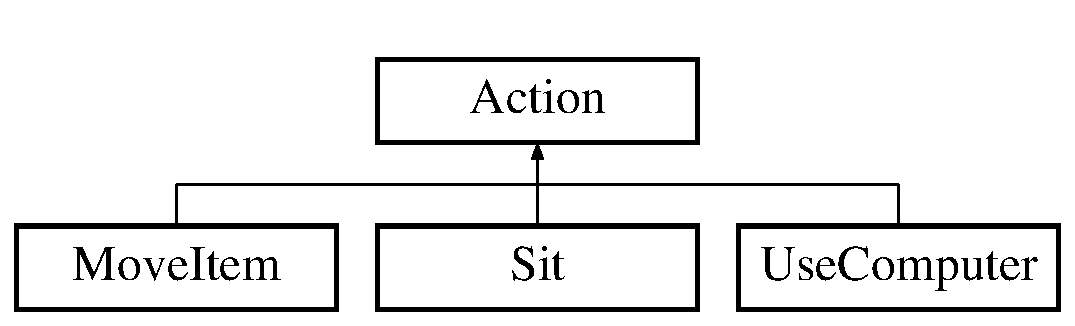
\includegraphics[height=2.000000cm]{class_action}
\end{center}
\end{figure}


\subsection{Detailed Description}
\hyperlink{class_action}{Action}. 

\begin{DoxyAuthor}{Author}
Hamish Carrier 
\end{DoxyAuthor}
\begin{DoxyDate}{Date}
10/11/2013 
\end{DoxyDate}


The documentation for this class was generated from the following file\-:\begin{DoxyCompactItemize}
\item 
A\-:/\-I\-T/\-Git\-Hub/\-I\-C\-T312/source/ogregraphics/\hyperlink{_action_manager_8h}{Action\-Manager.\-h}\end{DoxyCompactItemize}

\hypertarget{class_action_manager}{\section{Action\-Manager Class Reference}
\label{class_action_manager}\index{Action\-Manager@{Action\-Manager}}
}


Manager for actions.  




{\ttfamily \#include $<$Action\-Manager.\-h$>$}

\subsection*{Public Member Functions}
\begin{DoxyCompactItemize}
\item 
\hyperlink{class_action}{Action} $\ast$ \hyperlink{class_action_manager_ac0522de689b6f41724ebd2aca646646d}{Fetch\-Action} (Enum\-Space\-::\-Action\-Types Desired\-Action)
\begin{DoxyCompactList}\small\item\em Fetches an action. \end{DoxyCompactList}\item 
void \hyperlink{class_action_manager_a6ab448b8fb4a0df2dd9ee0887c5dfcef}{Initialise\-Action} (Enum\-Space\-::\-Action\-Types Action\-Type, int $\ast$Multipliers)
\begin{DoxyCompactList}\small\item\em Initialises the action. \end{DoxyCompactList}\item 
std\-::map\\*
$<$ Enum\-Space\-::\-Emotion\-Types, int $>$ \hyperlink{class_action_manager_a8e9097726d1dbeb537a1d64edd24fce8}{Get\-Emotion\-Multipliers} (Enum\-Space\-::\-Action\-Types Action\-Type)
\begin{DoxyCompactList}\small\item\em Gets emotion multipliers. \end{DoxyCompactList}\item 
void \hyperlink{class_action_manager_a75f119f905f44a55f7ca3bf2ccd00467}{Init} (void)
\begin{DoxyCompactList}\small\item\em Initialises this object. \end{DoxyCompactList}\end{DoxyCompactItemize}
\subsection*{Static Public Member Functions}
\begin{DoxyCompactItemize}
\item 
static \hyperlink{class_action_manager}{Action\-Manager} $\ast$ \hyperlink{class_action_manager_a91970883f9197898ed801f9a80b59595}{Get\-Instance} ()
\begin{DoxyCompactList}\small\item\em Gets the instance. \end{DoxyCompactList}\end{DoxyCompactItemize}


\subsection{Detailed Description}
Manager for actions. 

\begin{DoxyAuthor}{Author}
Hamish Carrier 
\end{DoxyAuthor}
\begin{DoxyDate}{Date}
10/11/2013 
\end{DoxyDate}


\subsection{Member Function Documentation}
\hypertarget{class_action_manager_ac0522de689b6f41724ebd2aca646646d}{\index{Action\-Manager@{Action\-Manager}!Fetch\-Action@{Fetch\-Action}}
\index{Fetch\-Action@{Fetch\-Action}!ActionManager@{Action\-Manager}}
\subsubsection[{Fetch\-Action}]{\setlength{\rightskip}{0pt plus 5cm}{\bf Action} $\ast$ Action\-Manager\-::\-Fetch\-Action (
\begin{DoxyParamCaption}
\item[{Enum\-Space\-::\-Action\-Types}]{Desired\-Action}
\end{DoxyParamCaption}
)}}\label{class_action_manager_ac0522de689b6f41724ebd2aca646646d}


Fetches an action. 

\begin{DoxyAuthor}{Author}
Hamish Carrier 
\end{DoxyAuthor}
\begin{DoxyDate}{Date}
10/11/2013
\end{DoxyDate}

\begin{DoxyParams}{Parameters}
{\em Desired\-Action} & The desired action.\\
\hline
\end{DoxyParams}
\begin{DoxyReturn}{Returns}
null if it fails, else the action. 
\end{DoxyReturn}
\hypertarget{class_action_manager_a8e9097726d1dbeb537a1d64edd24fce8}{\index{Action\-Manager@{Action\-Manager}!Get\-Emotion\-Multipliers@{Get\-Emotion\-Multipliers}}
\index{Get\-Emotion\-Multipliers@{Get\-Emotion\-Multipliers}!ActionManager@{Action\-Manager}}
\subsubsection[{Get\-Emotion\-Multipliers}]{\setlength{\rightskip}{0pt plus 5cm}std\-::map$<$ Enum\-Space\-::\-Emotion\-Types, int $>$ Action\-Manager\-::\-Get\-Emotion\-Multipliers (
\begin{DoxyParamCaption}
\item[{Enum\-Space\-::\-Action\-Types}]{Action\-Type}
\end{DoxyParamCaption}
)}}\label{class_action_manager_a8e9097726d1dbeb537a1d64edd24fce8}


Gets emotion multipliers. 

\begin{DoxyAuthor}{Author}
Hamish Carrier 
\end{DoxyAuthor}
\begin{DoxyDate}{Date}
10/11/2013
\end{DoxyDate}

\begin{DoxyParams}{Parameters}
{\em Action\-Type} & Type of the action.\\
\hline
\end{DoxyParams}
\begin{DoxyReturn}{Returns}
The emotion multipliers. 
\end{DoxyReturn}
\hypertarget{class_action_manager_a91970883f9197898ed801f9a80b59595}{\index{Action\-Manager@{Action\-Manager}!Get\-Instance@{Get\-Instance}}
\index{Get\-Instance@{Get\-Instance}!ActionManager@{Action\-Manager}}
\subsubsection[{Get\-Instance}]{\setlength{\rightskip}{0pt plus 5cm}static {\bf Action\-Manager} $\ast$ Action\-Manager\-::\-Get\-Instance (
\begin{DoxyParamCaption}
{}
\end{DoxyParamCaption}
)\hspace{0.3cm}{\ttfamily [static]}}}\label{class_action_manager_a91970883f9197898ed801f9a80b59595}


Gets the instance. 

\begin{DoxyAuthor}{Author}
Hamish Carrier 
\end{DoxyAuthor}
\begin{DoxyDate}{Date}
10/11/2013
\end{DoxyDate}
\begin{DoxyReturn}{Returns}
null if it fails, else the instance. 
\end{DoxyReturn}
\hypertarget{class_action_manager_a75f119f905f44a55f7ca3bf2ccd00467}{\index{Action\-Manager@{Action\-Manager}!Init@{Init}}
\index{Init@{Init}!ActionManager@{Action\-Manager}}
\subsubsection[{Init}]{\setlength{\rightskip}{0pt plus 5cm}void Action\-Manager\-::\-Init (
\begin{DoxyParamCaption}
\item[{void}]{}
\end{DoxyParamCaption}
)}}\label{class_action_manager_a75f119f905f44a55f7ca3bf2ccd00467}


Initialises this object. 

\begin{DoxyAuthor}{Author}
Hamish Carrier 
\end{DoxyAuthor}
\begin{DoxyDate}{Date}
10/11/2013 
\end{DoxyDate}
\hypertarget{class_action_manager_a6ab448b8fb4a0df2dd9ee0887c5dfcef}{\index{Action\-Manager@{Action\-Manager}!Initialise\-Action@{Initialise\-Action}}
\index{Initialise\-Action@{Initialise\-Action}!ActionManager@{Action\-Manager}}
\subsubsection[{Initialise\-Action}]{\setlength{\rightskip}{0pt plus 5cm}void Action\-Manager\-::\-Initialise\-Action (
\begin{DoxyParamCaption}
\item[{Enum\-Space\-::\-Action\-Types}]{Action\-Type, }
\item[{int $\ast$}]{Multipliers}
\end{DoxyParamCaption}
)}}\label{class_action_manager_a6ab448b8fb4a0df2dd9ee0887c5dfcef}


Initialises the action. 

\begin{DoxyAuthor}{Author}
Hamish Carrier 
\end{DoxyAuthor}
\begin{DoxyDate}{Date}
10/11/2013
\end{DoxyDate}

\begin{DoxyParams}[1]{Parameters}
 & {\em Action\-Type} & Type of the action. \\
\hline
\mbox{\tt in,out}  & {\em Multipliers} & If non-\/null, the multipliers. \\
\hline
\end{DoxyParams}


The documentation for this class was generated from the following files\-:\begin{DoxyCompactItemize}
\item 
A\-:/\-I\-T/\-Git\-Hub/\-I\-C\-T312/source/ogregraphics/\hyperlink{_action_manager_8h}{Action\-Manager.\-h}\item 
A\-:/\-I\-T/\-Git\-Hub/\-I\-C\-T312/source/ogregraphics/Action\-Manager.\-cpp\end{DoxyCompactItemize}

\hypertarget{class_a_i_manager}{\section{A\-I\-Manager Class Reference}
\label{class_a_i_manager}\index{A\-I\-Manager@{A\-I\-Manager}}
}
\subsection*{Public Member Functions}
\begin{DoxyCompactItemize}
\item 
\hypertarget{class_a_i_manager_af99b2cc614087185d6f8a74b8c80111b}{void {\bfseries Update\-A\-I} ()}\label{class_a_i_manager_af99b2cc614087185d6f8a74b8c80111b}

\item 
\hypertarget{class_a_i_manager_af7caaeaa220cf5f36e82c036b50ad378}{void {\bfseries Initialise} ()}\label{class_a_i_manager_af7caaeaa220cf5f36e82c036b50ad378}

\item 
\hypertarget{class_a_i_manager_a48977d671aed1b9e7d47deba33660b36}{void {\bfseries Add\-N\-P\-C} (\hyperlink{class_objects_1_1_i_object}{Objects\-::\-I\-Object} $\ast$Object\-Pointer)}\label{class_a_i_manager_a48977d671aed1b9e7d47deba33660b36}

\item 
\hypertarget{class_a_i_manager_adf5c673a55397d734aac9ddcb29dc1c0}{\hyperlink{class_n_p_c}{N\-P\-C} $\ast$ {\bfseries Get\-N\-P\-C} (int index)}\label{class_a_i_manager_adf5c673a55397d734aac9ddcb29dc1c0}

\end{DoxyCompactItemize}


The documentation for this class was generated from the following files\-:\begin{DoxyCompactItemize}
\item 
A\-:/\-I\-T/\-Git\-Hub/\-I\-C\-T312/source/ogregraphics/A\-I\-Manager.\-h\item 
A\-:/\-I\-T/\-Git\-Hub/\-I\-C\-T312/source/ogregraphics/A\-I\-Manager.\-cpp\end{DoxyCompactItemize}

\hypertarget{class_ogre_bullet_collisions_1_1_animated_mesh_to_shape_converter}{\section{Ogre\-Bullet\-Collisions\-:\-:Animated\-Mesh\-To\-Shape\-Converter Class Reference}
\label{class_ogre_bullet_collisions_1_1_animated_mesh_to_shape_converter}\index{Ogre\-Bullet\-Collisions\-::\-Animated\-Mesh\-To\-Shape\-Converter@{Ogre\-Bullet\-Collisions\-::\-Animated\-Mesh\-To\-Shape\-Converter}}
}
Inheritance diagram for Ogre\-Bullet\-Collisions\-:\-:Animated\-Mesh\-To\-Shape\-Converter\-:\begin{figure}[H]
\begin{center}
\leavevmode
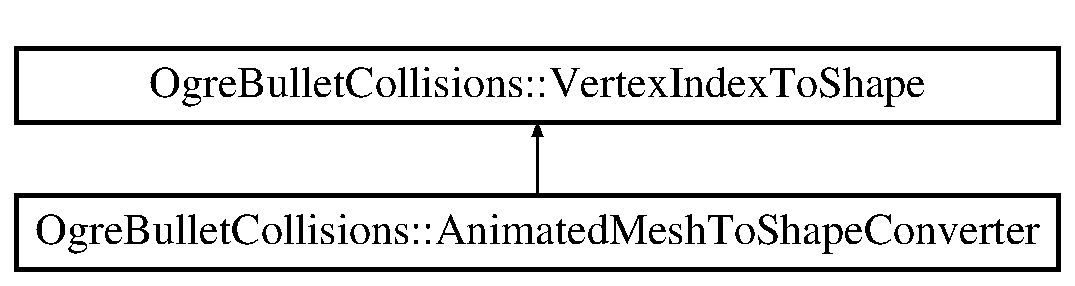
\includegraphics[height=2.000000cm]{class_ogre_bullet_collisions_1_1_animated_mesh_to_shape_converter}
\end{center}
\end{figure}
\subsection*{Public Member Functions}
\begin{DoxyCompactItemize}
\item 
\hypertarget{class_ogre_bullet_collisions_1_1_animated_mesh_to_shape_converter_aedf4c4317fe257fa248c584f73a5b07e}{{\bfseries Animated\-Mesh\-To\-Shape\-Converter} (Ogre\-::\-Entity $\ast$entity, const Ogre\-::\-Matrix4 \&transform=Ogre\-::\-Matrix4\-::\-I\-D\-E\-N\-T\-I\-T\-Y)}\label{class_ogre_bullet_collisions_1_1_animated_mesh_to_shape_converter_aedf4c4317fe257fa248c584f73a5b07e}

\item 
\hypertarget{class_ogre_bullet_collisions_1_1_animated_mesh_to_shape_converter_ad99910d169c2f27a64cbc32499d9a2f6}{void {\bfseries add\-Entity} (Ogre\-::\-Entity $\ast$entity, const Ogre\-::\-Matrix4 \&transform=Ogre\-::\-Matrix4\-::\-I\-D\-E\-N\-T\-I\-T\-Y)}\label{class_ogre_bullet_collisions_1_1_animated_mesh_to_shape_converter_ad99910d169c2f27a64cbc32499d9a2f6}

\item 
\hypertarget{class_ogre_bullet_collisions_1_1_animated_mesh_to_shape_converter_a26a59f1db578e3e08949d839646ee81c}{void {\bfseries add\-Mesh} (const Ogre\-::\-Mesh\-Ptr \&mesh, const Ogre\-::\-Matrix4 \&transform)}\label{class_ogre_bullet_collisions_1_1_animated_mesh_to_shape_converter_a26a59f1db578e3e08949d839646ee81c}

\item 
\hypertarget{class_ogre_bullet_collisions_1_1_animated_mesh_to_shape_converter_a0593a0e8cd5f076b15e8b4f60b3507f0}{Box\-Collision\-Shape $\ast$ {\bfseries create\-Aligned\-Box} (unsigned char bone, const Ogre\-::\-Vector3 \&bone\-Position, const Ogre\-::\-Quaternion \&bone\-Orientation)}\label{class_ogre_bullet_collisions_1_1_animated_mesh_to_shape_converter_a0593a0e8cd5f076b15e8b4f60b3507f0}

\item 
\hypertarget{class_ogre_bullet_collisions_1_1_animated_mesh_to_shape_converter_a0e58a873f3b72749bdd764035a54a4f1}{Box\-Collision\-Shape $\ast$ {\bfseries create\-Oriented\-Box} (unsigned char bone, const Ogre\-::\-Vector3 \&bone\-Position, const Ogre\-::\-Quaternion \&bone\-Orientation)}\label{class_ogre_bullet_collisions_1_1_animated_mesh_to_shape_converter_a0e58a873f3b72749bdd764035a54a4f1}

\item 
\hypertarget{class_ogre_bullet_collisions_1_1_animated_mesh_to_shape_converter_afa5359d06b4d8c8cd65484070976218d}{Capsule\-Collision\-Shape $\ast$ {\bfseries create\-Oriented\-Capsule\-Collision\-Shape} (unsigned char bone, const Ogre\-::\-Vector3 \&bone\-Position, const Ogre\-::\-Quaternion \&bone\-Orientation)}\label{class_ogre_bullet_collisions_1_1_animated_mesh_to_shape_converter_afa5359d06b4d8c8cd65484070976218d}

\end{DoxyCompactItemize}
\subsection*{Protected Member Functions}
\begin{DoxyCompactItemize}
\item 
\hypertarget{class_ogre_bullet_collisions_1_1_animated_mesh_to_shape_converter_a4d89a32d20322dc74579240779689573}{bool {\bfseries get\-Bone\-Vertices} (unsigned char bone, unsigned int \&vertex\-\_\-count, Ogre\-::\-Vector3 $\ast$\&vertices, const Ogre\-::\-Vector3 \&bone\-Position)}\label{class_ogre_bullet_collisions_1_1_animated_mesh_to_shape_converter_a4d89a32d20322dc74579240779689573}

\item 
\hypertarget{class_ogre_bullet_collisions_1_1_animated_mesh_to_shape_converter_ab2f46f4182bf24d3dad8a77c17514980}{bool {\bfseries get\-Oriented\-Box} (unsigned char bone, const Ogre\-::\-Vector3 \&bone\-Position, const Ogre\-::\-Quaternion \&bone\-Orientation, Ogre\-::\-Vector3 \&extents, Ogre\-::\-Vector3 $\ast$axis, Ogre\-::\-Vector3 \&center)}\label{class_ogre_bullet_collisions_1_1_animated_mesh_to_shape_converter_ab2f46f4182bf24d3dad8a77c17514980}

\end{DoxyCompactItemize}
\subsection*{Protected Attributes}
\begin{DoxyCompactItemize}
\item 
\hypertarget{class_ogre_bullet_collisions_1_1_animated_mesh_to_shape_converter_ad20b11e7c144a4b9198a18a6b05107d5}{Ogre\-::\-Entity $\ast$ {\bfseries m\-Entity}}\label{class_ogre_bullet_collisions_1_1_animated_mesh_to_shape_converter_ad20b11e7c144a4b9198a18a6b05107d5}

\item 
\hypertarget{class_ogre_bullet_collisions_1_1_animated_mesh_to_shape_converter_a4599877a3c3184c2a75668616ac638e9}{Ogre\-::\-Scene\-Node $\ast$ {\bfseries m\-Node}}\label{class_ogre_bullet_collisions_1_1_animated_mesh_to_shape_converter_a4599877a3c3184c2a75668616ac638e9}

\item 
\hypertarget{class_ogre_bullet_collisions_1_1_animated_mesh_to_shape_converter_a53c5f39e5ea92ac33e0e4b16a0896da3}{Ogre\-::\-Vector3 $\ast$ {\bfseries m\-Transformed\-Vertices\-Temp}}\label{class_ogre_bullet_collisions_1_1_animated_mesh_to_shape_converter_a53c5f39e5ea92ac33e0e4b16a0896da3}

\item 
\hypertarget{class_ogre_bullet_collisions_1_1_animated_mesh_to_shape_converter_a794b6ca934c798f46e5bd4b5fd421016}{size\-\_\-t {\bfseries m\-Transformed\-Vertices\-Temp\-Size}}\label{class_ogre_bullet_collisions_1_1_animated_mesh_to_shape_converter_a794b6ca934c798f46e5bd4b5fd421016}

\end{DoxyCompactItemize}


The documentation for this class was generated from the following files\-:\begin{DoxyCompactItemize}
\item 
A\-:/\-I\-T/\-Git\-Hub/\-I\-C\-T312/source/ogregraphics/Ogre\-Bullet\-Collisions\-Mesh\-To\-Shape\-Converter.\-h\item 
A\-:/\-I\-T/\-Git\-Hub/\-I\-C\-T312/source/ogregraphics/Ogre\-Bullet\-Collisions\-Mesh\-To\-Shape\-Converter.\-cpp\end{DoxyCompactItemize}

\hypertarget{class_bad}{\section{Bad Class Reference}
\label{class_bad}\index{Bad@{Bad}}
}


\hyperlink{class_bad}{Bad}.  




{\ttfamily \#include $<$Bad.\-h$>$}

Inheritance diagram for Bad\-:\begin{figure}[H]
\begin{center}
\leavevmode
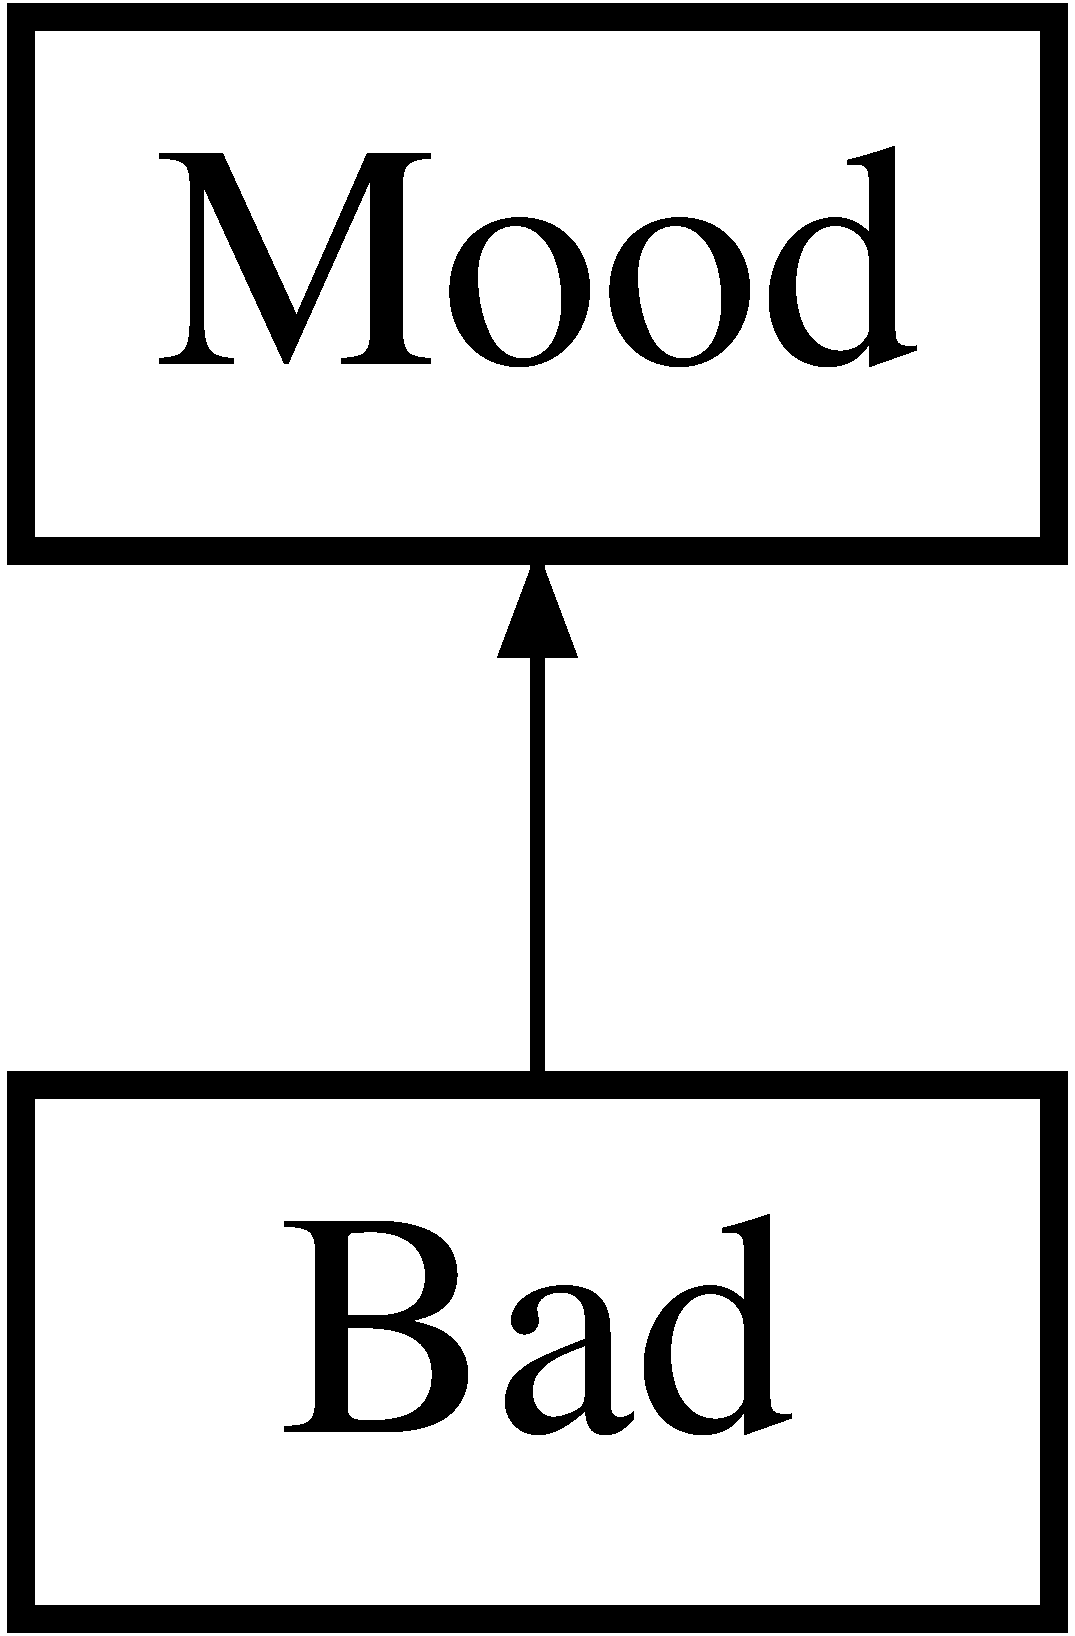
\includegraphics[height=2.000000cm]{class_bad}
\end{center}
\end{figure}
\subsection*{Public Member Functions}
\begin{DoxyCompactItemize}
\item 
\hyperlink{class_bad_a183ebda2cf376b54889da8da10af8533}{Bad} (void)
\begin{DoxyCompactList}\small\item\em Default constructor. \end{DoxyCompactList}\item 
\hyperlink{class_bad_a124c764cd2b1bad6313bc7b3c0cd15c9}{$\sim$\-Bad} (void)
\begin{DoxyCompactList}\small\item\em Destructor. \end{DoxyCompactList}\end{DoxyCompactItemize}


\subsection{Detailed Description}
\hyperlink{class_bad}{Bad}. 

\begin{DoxyAuthor}{Author}
Hamish Carrier 
\end{DoxyAuthor}
\begin{DoxyDate}{Date}
10/11/2013 
\end{DoxyDate}


\subsection{Constructor \& Destructor Documentation}
\hypertarget{class_bad_a183ebda2cf376b54889da8da10af8533}{\index{Bad@{Bad}!Bad@{Bad}}
\index{Bad@{Bad}!Bad@{Bad}}
\subsubsection[{Bad}]{\setlength{\rightskip}{0pt plus 5cm}Bad\-::\-Bad (
\begin{DoxyParamCaption}
\item[{void}]{}
\end{DoxyParamCaption}
)}}\label{class_bad_a183ebda2cf376b54889da8da10af8533}


Default constructor. 

\begin{DoxyAuthor}{Author}
Hamish Carrier 
\end{DoxyAuthor}
\begin{DoxyDate}{Date}
10/11/2013 
\end{DoxyDate}
\hypertarget{class_bad_a124c764cd2b1bad6313bc7b3c0cd15c9}{\index{Bad@{Bad}!$\sim$\-Bad@{$\sim$\-Bad}}
\index{$\sim$\-Bad@{$\sim$\-Bad}!Bad@{Bad}}
\subsubsection[{$\sim$\-Bad}]{\setlength{\rightskip}{0pt plus 5cm}Bad\-::$\sim$\-Bad (
\begin{DoxyParamCaption}
\item[{void}]{}
\end{DoxyParamCaption}
)}}\label{class_bad_a124c764cd2b1bad6313bc7b3c0cd15c9}


Destructor. 

\begin{DoxyAuthor}{Author}
Hamish Carrier 
\end{DoxyAuthor}
\begin{DoxyDate}{Date}
10/11/2013 
\end{DoxyDate}


The documentation for this class was generated from the following files\-:\begin{DoxyCompactItemize}
\item 
A\-:/\-I\-T/\-Git\-Hub/\-I\-C\-T312/source/ogregraphics/\hyperlink{_bad_8h}{Bad.\-h}\item 
A\-:/\-I\-T/\-Git\-Hub/\-I\-C\-T312/source/ogregraphics/Bad.\-cpp\end{DoxyCompactItemize}

\hypertarget{class_c_hull}{\section{C\-Hull Class Reference}
\label{class_c_hull}\index{C\-Hull@{C\-Hull}}
}
\subsection*{Public Member Functions}
\begin{DoxyCompactItemize}
\item 
\hypertarget{class_c_hull_ac3d6207a87359bb1c0d90e945b28d85b}{{\bfseries C\-Hull} (const \hyperlink{class_convex_decomposition_1_1_convex_result}{Convex\-Result} \&result)}\label{class_c_hull_ac3d6207a87359bb1c0d90e945b28d85b}

\item 
\hypertarget{class_c_hull_a30a0e6b490d7fd5c3d54090ff01304a0}{bool {\bfseries overlap} (const \hyperlink{class_c_hull}{C\-Hull} \&h) const }\label{class_c_hull_a30a0e6b490d7fd5c3d54090ff01304a0}

\end{DoxyCompactItemize}
\subsection*{Public Attributes}
\begin{DoxyCompactItemize}
\item 
\hypertarget{class_c_hull_a7e2b0c242e99ce07586426877428158b}{float {\bfseries m\-Min} \mbox{[}3\mbox{]}}\label{class_c_hull_a7e2b0c242e99ce07586426877428158b}

\item 
\hypertarget{class_c_hull_ae279e2bb3b7b3b3a2a85dadd362f6b62}{float {\bfseries m\-Max} \mbox{[}3\mbox{]}}\label{class_c_hull_ae279e2bb3b7b3b3a2a85dadd362f6b62}

\item 
\hypertarget{class_c_hull_ad8ef82af9ddfbbabc76486aae1c0a8cd}{float {\bfseries m\-Volume}}\label{class_c_hull_ad8ef82af9ddfbbabc76486aae1c0a8cd}

\item 
\hypertarget{class_c_hull_aced64e719b25f3f3fadbccc03c0e3531}{float {\bfseries m\-Diagonal}}\label{class_c_hull_aced64e719b25f3f3fadbccc03c0e3531}

\item 
\hypertarget{class_c_hull_a3c7d7fe1ad593540c4ba27564dae9c69}{\hyperlink{class_convex_decomposition_1_1_convex_result}{Convex\-Result} $\ast$ {\bfseries m\-Result}}\label{class_c_hull_a3c7d7fe1ad593540c4ba27564dae9c69}

\end{DoxyCompactItemize}


The documentation for this class was generated from the following files\-:\begin{DoxyCompactItemize}
\item 
A\-:/\-I\-T/\-Git\-Hub/\-I\-C\-T312/source/ogregraphics/Convex\-Builder.\-h\item 
A\-:/\-I\-T/\-Git\-Hub/\-I\-C\-T312/source/ogregraphics/Convex\-Builder.\-cpp\end{DoxyCompactItemize}

\hypertarget{class_c_hull_sort}{\section{C\-Hull\-Sort Class Reference}
\label{class_c_hull_sort}\index{C\-Hull\-Sort@{C\-Hull\-Sort}}
}
\subsection*{Public Member Functions}
\begin{DoxyCompactItemize}
\item 
\hypertarget{class_c_hull_sort_aa5de23224fa2388336df7b6bccc94d59}{bool {\bfseries operator()} (const \hyperlink{class_c_hull}{C\-Hull} $\ast$a, const \hyperlink{class_c_hull}{C\-Hull} $\ast$b) const }\label{class_c_hull_sort_aa5de23224fa2388336df7b6bccc94d59}

\end{DoxyCompactItemize}


The documentation for this class was generated from the following file\-:\begin{DoxyCompactItemize}
\item 
A\-:/\-I\-T/\-Git\-Hub/\-I\-C\-T312/source/ogregraphics/Convex\-Builder.\-h\end{DoxyCompactItemize}

\hypertarget{class_closed_set}{\section{Closed\-Set Class Reference}
\label{class_closed_set}\index{Closed\-Set@{Closed\-Set}}
}
\subsection*{Public Member Functions}
\begin{DoxyCompactItemize}
\item 
\hypertarget{class_closed_set_acf6657729a6bbc37fb44c8c3c582185c}{{\bfseries Closed\-Set} (\hyperlink{classmicropather_1_1_graph}{Graph} $\ast$\-\_\-graph)}\label{class_closed_set_acf6657729a6bbc37fb44c8c3c582185c}

\item 
\hypertarget{class_closed_set_a76c0f439e938b9229f5adff9cd89ab71}{void {\bfseries Add} (\hyperlink{classmicropather_1_1_path_node}{Path\-Node} $\ast$p\-Node)}\label{class_closed_set_a76c0f439e938b9229f5adff9cd89ab71}

\item 
\hypertarget{class_closed_set_a6aae1d2c46516088ec98131508b9103a}{void {\bfseries Remove} (\hyperlink{classmicropather_1_1_path_node}{Path\-Node} $\ast$p\-Node)}\label{class_closed_set_a6aae1d2c46516088ec98131508b9103a}

\end{DoxyCompactItemize}


The documentation for this class was generated from the following file\-:\begin{DoxyCompactItemize}
\item 
A\-:/\-I\-T/\-Git\-Hub/\-I\-C\-T312/source/ogregraphics/micropather.\-cpp\end{DoxyCompactItemize}

\hypertarget{class_collision_object}{\section{Collision\-Object Class Reference}
\label{class_collision_object}\index{Collision\-Object@{Collision\-Object}}
}


Collision object.  




{\ttfamily \#include $<$Collision\-Object.\-h$>$}

\subsection*{Public Member Functions}
\begin{DoxyCompactItemize}
\item 
\hyperlink{class_collision_object_a808493e22b7d12937464f4244ad7966a}{Collision\-Object} ()
\begin{DoxyCompactList}\small\item\em Default constructer. \end{DoxyCompactList}\item 
void \hyperlink{class_collision_object_ad556e9d6698b245c7691db5a2205ae6c}{Add\-Mesh\-Shape} (Ogre\-::\-Entity $\ast$Ent)
\begin{DoxyCompactList}\small\item\em Adds a mesh shape based off the Ogre mesh. \end{DoxyCompactList}\item 
void \hyperlink{class_collision_object_a11fbb95c3d71c6fe1b8d35cb512ba173}{Add\-Mesh\-Shape\-With\-Offset} (Ogre\-::\-Entity $\ast$Ent, Ogre\-::\-Vector3 Offset)
\begin{DoxyCompactList}\small\item\em Adds a mesh shape based off the Ogre mesh with an offset to correctly position center of gravity. \end{DoxyCompactList}\item 
void \hyperlink{class_collision_object_a41ba682403cabbaad6a9c5d33bb2e62c}{Add\-Box\-Shape} (float x\-Length, float y\-Length, float z\-Length)
\begin{DoxyCompactList}\small\item\em Adds a box shape. \end{DoxyCompactList}\item 
void \hyperlink{class_collision_object_a0df8a4a05b49e3fde9be693ac2187bd2}{Add\-Sphere\-Shape} (float Radius)
\begin{DoxyCompactList}\small\item\em Adds a sphere shape. \end{DoxyCompactList}\item 
void \hyperlink{class_collision_object_a0c9429cee147f5c5d23b36b66151348c}{Set\-Position} (float xpos, float ypos, float zpos)
\begin{DoxyCompactList}\small\item\em Sets the object position via 3 floats. \end{DoxyCompactList}\item 
void \hyperlink{class_collision_object_a42b7b3f3af11bcc551cb05600af39ae6}{Set\-Position} (Ogre\-::\-Vector3 vecpos)
\begin{DoxyCompactList}\small\item\em Sets the object position via an Ogre Vector3. \end{DoxyCompactList}\item 
\hypertarget{class_collision_object_a6bf3394037d2d5a49aae57bbf98126bf}{void {\bfseries Add\-Sphere\-Shape} (Ogre\-::\-Entity $\ast$Ent)}\label{class_collision_object_a6bf3394037d2d5a49aae57bbf98126bf}

\item 
void \hyperlink{class_collision_object_a87925eeb7b7453dac768782671db7498}{Move\-Object} (Ogre\-::\-Vector3 vec)
\begin{DoxyCompactList}\small\item\em Move object. \end{DoxyCompactList}\item 
void \hyperlink{class_collision_object_aa2aeac308fb44ae4829e4f2a55890c56}{Set\-Object\-Orientation} (float x, float y, float z, float Degrees)
\begin{DoxyCompactList}\small\item\em Sets the objects orientation. \end{DoxyCompactList}\item 
void \hyperlink{class_collision_object_aca121d7ab9ae0e0295c6b44de37d2a54}{Set\-Object\-Orientation} (Ogre\-::\-Quaternion quat)
\begin{DoxyCompactList}\small\item\em Set the object orientation by quaternion. \end{DoxyCompactList}\item 
void \hyperlink{class_collision_object_a59db2ca5c552ebd20faf2ac4dae19198}{Set\-User\-Pointer} (void $\ast$obj)
\begin{DoxyCompactList}\small\item\em Set the objects void pointer. \end{DoxyCompactList}\item 
void \hyperlink{class_collision_object_a3c091aaffc9199127d88a090405f5012}{Set\-Scale} (float xs, float ys, float zs)
\begin{DoxyCompactList}\small\item\em Sets the scale of the object. \end{DoxyCompactList}\item 
\hypertarget{class_collision_object_a8271ca0e023aeebb34be4c858e18005a}{bt\-Collision\-Object $\ast$ {\bfseries Get\-Collision\-Object} ()}\label{class_collision_object_a8271ca0e023aeebb34be4c858e18005a}

\item 
Ogre\-::\-Vector3 \hyperlink{class_collision_object_aee08b61704b439a2e8451e1e777ce99d}{Get\-Object\-Position} ()
\begin{DoxyCompactList}\small\item\em return the position vector of the object \end{DoxyCompactList}\item 
\hypertarget{class_collision_object_a9af163a4ca7353814e3da7b1241c8751}{void {\bfseries Add\-Box\-Mesh} (Ogre\-::\-Entity $\ast$Ent)}\label{class_collision_object_a9af163a4ca7353814e3da7b1241c8751}

\end{DoxyCompactItemize}
\subsection*{Public Attributes}
\begin{DoxyCompactItemize}
\item 
\hypertarget{class_collision_object_a463ac6145a03138cdcb60efcff9c756b}{bt\-Convex\-Hull\-Shape $\ast$ \hyperlink{class_collision_object_a463ac6145a03138cdcb60efcff9c756b}{convex\-Shape}}\label{class_collision_object_a463ac6145a03138cdcb60efcff9c756b}

\begin{DoxyCompactList}\small\item\em The convex shape. \end{DoxyCompactList}\end{DoxyCompactItemize}


\subsection{Detailed Description}
Collision object. 

\begin{DoxyAuthor}{Author}
Arran Ford 
\end{DoxyAuthor}
\begin{DoxyDate}{Date}
16/09/2013 
\end{DoxyDate}


\subsection{Constructor \& Destructor Documentation}
\hypertarget{class_collision_object_a808493e22b7d12937464f4244ad7966a}{\index{Collision\-Object@{Collision\-Object}!Collision\-Object@{Collision\-Object}}
\index{Collision\-Object@{Collision\-Object}!CollisionObject@{Collision\-Object}}
\subsubsection[{Collision\-Object}]{\setlength{\rightskip}{0pt plus 5cm}void Collision\-Object\-::\-Collision\-Object (
\begin{DoxyParamCaption}
{}
\end{DoxyParamCaption}
)}}\label{class_collision_object_a808493e22b7d12937464f4244ad7966a}


Default constructer. 

\begin{DoxyAuthor}{Author}
Arran Ford 
\end{DoxyAuthor}
\begin{DoxyDate}{Date}
16/09/2013 
\end{DoxyDate}


\subsection{Member Function Documentation}
\hypertarget{class_collision_object_a41ba682403cabbaad6a9c5d33bb2e62c}{\index{Collision\-Object@{Collision\-Object}!Add\-Box\-Shape@{Add\-Box\-Shape}}
\index{Add\-Box\-Shape@{Add\-Box\-Shape}!CollisionObject@{Collision\-Object}}
\subsubsection[{Add\-Box\-Shape}]{\setlength{\rightskip}{0pt plus 5cm}void Collision\-Object\-::\-Add\-Box\-Shape (
\begin{DoxyParamCaption}
\item[{float}]{x\-Length, }
\item[{float}]{y\-Length, }
\item[{float}]{z\-Length}
\end{DoxyParamCaption}
)}}\label{class_collision_object_a41ba682403cabbaad6a9c5d33bb2e62c}


Adds a box shape. 

\begin{DoxyAuthor}{Author}
Arran Ford 
\end{DoxyAuthor}
\begin{DoxyDate}{Date}
31/10/2013
\end{DoxyDate}

\begin{DoxyParams}{Parameters}
{\em x\-Length} & The length. \\
\hline
{\em y\-Length} & The length. \\
\hline
{\em z\-Length} & The length. \\
\hline
\end{DoxyParams}
\hypertarget{class_collision_object_ad556e9d6698b245c7691db5a2205ae6c}{\index{Collision\-Object@{Collision\-Object}!Add\-Mesh\-Shape@{Add\-Mesh\-Shape}}
\index{Add\-Mesh\-Shape@{Add\-Mesh\-Shape}!CollisionObject@{Collision\-Object}}
\subsubsection[{Add\-Mesh\-Shape}]{\setlength{\rightskip}{0pt plus 5cm}void Collision\-Object\-::\-Add\-Mesh\-Shape (
\begin{DoxyParamCaption}
\item[{Ogre\-::\-Entity $\ast$}]{Ent}
\end{DoxyParamCaption}
)}}\label{class_collision_object_ad556e9d6698b245c7691db5a2205ae6c}


Adds a mesh shape based off the Ogre mesh. 

\begin{DoxyAuthor}{Author}
Arran Ford 
\end{DoxyAuthor}
\begin{DoxyDate}{Date}
20/10/2013
\end{DoxyDate}

\begin{DoxyParams}{Parameters}
{\em Radius} & The radius. \\
\hline
\end{DoxyParams}
\hypertarget{class_collision_object_a11fbb95c3d71c6fe1b8d35cb512ba173}{\index{Collision\-Object@{Collision\-Object}!Add\-Mesh\-Shape\-With\-Offset@{Add\-Mesh\-Shape\-With\-Offset}}
\index{Add\-Mesh\-Shape\-With\-Offset@{Add\-Mesh\-Shape\-With\-Offset}!CollisionObject@{Collision\-Object}}
\subsubsection[{Add\-Mesh\-Shape\-With\-Offset}]{\setlength{\rightskip}{0pt plus 5cm}void Collision\-Object\-::\-Add\-Mesh\-Shape\-With\-Offset (
\begin{DoxyParamCaption}
\item[{Ogre\-::\-Entity $\ast$}]{Ent, }
\item[{Ogre\-::\-Vector3}]{Offset}
\end{DoxyParamCaption}
)}}\label{class_collision_object_a11fbb95c3d71c6fe1b8d35cb512ba173}


Adds a mesh shape based off the Ogre mesh with an offset to correctly position center of gravity. 

\begin{DoxyAuthor}{Author}
Arran Ford 
\end{DoxyAuthor}
\begin{DoxyDate}{Date}
20/10/2013
\end{DoxyDate}

\begin{DoxyParams}{Parameters}
{\em ent} & the Ogre entity \\
\hline
{\em Offset} & the offset vector \\
\hline
\end{DoxyParams}
\hypertarget{class_collision_object_a0df8a4a05b49e3fde9be693ac2187bd2}{\index{Collision\-Object@{Collision\-Object}!Add\-Sphere\-Shape@{Add\-Sphere\-Shape}}
\index{Add\-Sphere\-Shape@{Add\-Sphere\-Shape}!CollisionObject@{Collision\-Object}}
\subsubsection[{Add\-Sphere\-Shape}]{\setlength{\rightskip}{0pt plus 5cm}void Collision\-Object\-::\-Add\-Sphere\-Shape (
\begin{DoxyParamCaption}
\item[{float}]{Radius}
\end{DoxyParamCaption}
)}}\label{class_collision_object_a0df8a4a05b49e3fde9be693ac2187bd2}


Adds a sphere shape. 

\begin{DoxyAuthor}{Author}
Arran Ford 
\end{DoxyAuthor}
\begin{DoxyDate}{Date}
16/09/2013
\end{DoxyDate}

\begin{DoxyParams}{Parameters}
{\em Radius} & The radius. \\
\hline
\end{DoxyParams}
\hypertarget{class_collision_object_aee08b61704b439a2e8451e1e777ce99d}{\index{Collision\-Object@{Collision\-Object}!Get\-Object\-Position@{Get\-Object\-Position}}
\index{Get\-Object\-Position@{Get\-Object\-Position}!CollisionObject@{Collision\-Object}}
\subsubsection[{Get\-Object\-Position}]{\setlength{\rightskip}{0pt plus 5cm}Ogre\-::\-Vector3 Collision\-Object\-::\-Ogre\-::\-Vector3 Collision\-Object\-::\-Get\-Object\-Position (
\begin{DoxyParamCaption}
{}
\end{DoxyParamCaption}
)}}\label{class_collision_object_aee08b61704b439a2e8451e1e777ce99d}


return the position vector of the object 

\begin{DoxyAuthor}{Author}
Arran Ford 
\end{DoxyAuthor}
\begin{DoxyDate}{Date}
31/10/2013 
\end{DoxyDate}
\hypertarget{class_collision_object_a87925eeb7b7453dac768782671db7498}{\index{Collision\-Object@{Collision\-Object}!Move\-Object@{Move\-Object}}
\index{Move\-Object@{Move\-Object}!CollisionObject@{Collision\-Object}}
\subsubsection[{Move\-Object}]{\setlength{\rightskip}{0pt plus 5cm}void Collision\-Object\-::\-Move\-Object (
\begin{DoxyParamCaption}
\item[{Ogre\-::\-Vector3}]{vec}
\end{DoxyParamCaption}
)}}\label{class_collision_object_a87925eeb7b7453dac768782671db7498}


Move object. 

\begin{DoxyAuthor}{Author}
Arran Ford 
\end{DoxyAuthor}
\begin{DoxyDate}{Date}
16/09/2013
\end{DoxyDate}

\begin{DoxyParams}{Parameters}
{\em vec} & The vector.\\
\hline
\end{DoxyParams}
\begin{DoxyAuthor}{Author}
Arran Ford 
\end{DoxyAuthor}
\begin{DoxyDate}{Date}
31/10/2013
\end{DoxyDate}

\begin{DoxyParams}{Parameters}
{\em vec} & The vector. \\
\hline
\end{DoxyParams}
\hypertarget{class_collision_object_aa2aeac308fb44ae4829e4f2a55890c56}{\index{Collision\-Object@{Collision\-Object}!Set\-Object\-Orientation@{Set\-Object\-Orientation}}
\index{Set\-Object\-Orientation@{Set\-Object\-Orientation}!CollisionObject@{Collision\-Object}}
\subsubsection[{Set\-Object\-Orientation}]{\setlength{\rightskip}{0pt plus 5cm}void Collision\-Object\-::\-Set\-Object\-Orientation (
\begin{DoxyParamCaption}
\item[{float}]{x, }
\item[{float}]{y, }
\item[{float}]{z, }
\item[{float}]{Degrees}
\end{DoxyParamCaption}
)}}\label{class_collision_object_aa2aeac308fb44ae4829e4f2a55890c56}


Sets the objects orientation. 

\begin{DoxyAuthor}{Author}
Arran Ford 
\end{DoxyAuthor}
\begin{DoxyDate}{Date}
31/10/2013
\end{DoxyDate}

\begin{DoxyParams}{Parameters}
{\em Degrees} & The amount in degrees to rotate around the defined axis. \\
\hline
{\em x} & the x portion of the rotation axis \\
\hline
{\em y} & the y portion of the rotation axis \\
\hline
{\em z} & the z portion of the rotation axis \\
\hline
\end{DoxyParams}
\hypertarget{class_collision_object_aca121d7ab9ae0e0295c6b44de37d2a54}{\index{Collision\-Object@{Collision\-Object}!Set\-Object\-Orientation@{Set\-Object\-Orientation}}
\index{Set\-Object\-Orientation@{Set\-Object\-Orientation}!CollisionObject@{Collision\-Object}}
\subsubsection[{Set\-Object\-Orientation}]{\setlength{\rightskip}{0pt plus 5cm}void Collision\-Object\-::\-Set\-Object\-Orientation (
\begin{DoxyParamCaption}
\item[{Ogre\-::\-Quaternion}]{quat}
\end{DoxyParamCaption}
)}}\label{class_collision_object_aca121d7ab9ae0e0295c6b44de37d2a54}


Set the object orientation by quaternion. 

\begin{DoxyAuthor}{Author}
Arran Ford 
\end{DoxyAuthor}
\begin{DoxyDate}{Date}
31/10/2013
\end{DoxyDate}

\begin{DoxyParams}{Parameters}
{\em quat} & The Quaternion defining the objects new orientation \\
\hline
\end{DoxyParams}
\hypertarget{class_collision_object_a0c9429cee147f5c5d23b36b66151348c}{\index{Collision\-Object@{Collision\-Object}!Set\-Position@{Set\-Position}}
\index{Set\-Position@{Set\-Position}!CollisionObject@{Collision\-Object}}
\subsubsection[{Set\-Position}]{\setlength{\rightskip}{0pt plus 5cm}void Collision\-Object\-::\-Set\-Position (
\begin{DoxyParamCaption}
\item[{float}]{xpox, }
\item[{float}]{ypoz, }
\item[{float}]{zpos}
\end{DoxyParamCaption}
)}}\label{class_collision_object_a0c9429cee147f5c5d23b36b66151348c}


Sets the object position via 3 floats. 

\begin{DoxyAuthor}{Author}
Arran Ford 
\end{DoxyAuthor}
\begin{DoxyDate}{Date}
16/09/2013
\end{DoxyDate}

\begin{DoxyParams}{Parameters}
{\em xpos} & Position on the x axis. \\
\hline
{\em ypos} & Position on the y axis \\
\hline
{\em zpos} & Position on the z axis \\
\hline
\end{DoxyParams}
\hypertarget{class_collision_object_a42b7b3f3af11bcc551cb05600af39ae6}{\index{Collision\-Object@{Collision\-Object}!Set\-Position@{Set\-Position}}
\index{Set\-Position@{Set\-Position}!CollisionObject@{Collision\-Object}}
\subsubsection[{Set\-Position}]{\setlength{\rightskip}{0pt plus 5cm}void Collision\-Object\-::\-Set\-Position (
\begin{DoxyParamCaption}
\item[{Ogre\-::\-Vector3}]{vecpos}
\end{DoxyParamCaption}
)}}\label{class_collision_object_a42b7b3f3af11bcc551cb05600af39ae6}


Sets the object position via an Ogre Vector3. 

\begin{DoxyAuthor}{Author}
Arran Ford 
\end{DoxyAuthor}
\begin{DoxyDate}{Date}
16/09/2013
\end{DoxyDate}

\begin{DoxyParams}{Parameters}
{\em vecpos} & the Ogre Vector that determines new object location \\
\hline
\end{DoxyParams}
\hypertarget{class_collision_object_a3c091aaffc9199127d88a090405f5012}{\index{Collision\-Object@{Collision\-Object}!Set\-Scale@{Set\-Scale}}
\index{Set\-Scale@{Set\-Scale}!CollisionObject@{Collision\-Object}}
\subsubsection[{Set\-Scale}]{\setlength{\rightskip}{0pt plus 5cm}void Collision\-Object\-::\-Set\-Scale (
\begin{DoxyParamCaption}
\item[{float}]{xs, }
\item[{float}]{ys, }
\item[{float}]{zs}
\end{DoxyParamCaption}
)}}\label{class_collision_object_a3c091aaffc9199127d88a090405f5012}


Sets the scale of the object. 

\begin{DoxyAuthor}{Author}
Arran Ford 
\end{DoxyAuthor}
\begin{DoxyDate}{Date}
31/10/2013
\end{DoxyDate}

\begin{DoxyParams}{Parameters}
{\em xs} & the scale along x axis \\
\hline
{\em ys} & the scale along y axis \\
\hline
{\em zs} & the scale along z axis \\
\hline
\end{DoxyParams}
\hypertarget{class_collision_object_a59db2ca5c552ebd20faf2ac4dae19198}{\index{Collision\-Object@{Collision\-Object}!Set\-User\-Pointer@{Set\-User\-Pointer}}
\index{Set\-User\-Pointer@{Set\-User\-Pointer}!CollisionObject@{Collision\-Object}}
\subsubsection[{Set\-User\-Pointer}]{\setlength{\rightskip}{0pt plus 5cm}void Collision\-Object\-::\-Set\-User\-Pointer (
\begin{DoxyParamCaption}
\item[{void $\ast$}]{obj}
\end{DoxyParamCaption}
)}}\label{class_collision_object_a59db2ca5c552ebd20faf2ac4dae19198}


Set the objects void pointer. 

\begin{DoxyAuthor}{Author}
Arran Ford 
\end{DoxyAuthor}
\begin{DoxyDate}{Date}
31/10/2013
\end{DoxyDate}

\begin{DoxyParams}{Parameters}
{\em obj} & The object the void pointer will point to. \\
\hline
\end{DoxyParams}


The documentation for this class was generated from the following files\-:\begin{DoxyCompactItemize}
\item 
A\-:/\-I\-T/\-Git\-Hub/\-I\-C\-T312/source/ogregraphics/\hyperlink{_collision_object_8h}{Collision\-Object.\-h}\item 
A\-:/\-I\-T/\-Git\-Hub/\-I\-C\-T312/source/ogregraphics/Collision\-Object.\-cpp\end{DoxyCompactItemize}

\hypertarget{class_collision_world_singleton}{\section{Collision\-World\-Singleton Class Reference}
\label{class_collision_world_singleton}\index{Collision\-World\-Singleton@{Collision\-World\-Singleton}}
}


Collision world singleton.  




{\ttfamily \#include $<$Collision\-World\-Singleton.\-h$>$}

\subsection*{Public Member Functions}
\begin{DoxyCompactItemize}
\item 
\hypertarget{class_collision_world_singleton_a7b73e1b5f14b7b48d049f81a374d4772}{void {\bfseries Set\-Up\-Debug} ()}\label{class_collision_world_singleton_a7b73e1b5f14b7b48d049f81a374d4772}

\item 
void \hyperlink{class_collision_world_singleton_a6f2803fe6954a758a065718929103282}{Add\-Object} (bt\-Collision\-Object $\ast$colobj)
\begin{DoxyCompactList}\small\item\em Adds an object. \end{DoxyCompactList}\item 
void \hyperlink{class_collision_world_singleton_a4c8e153ddb2ac08f21eaa181741c7521}{Check\-Collision} ()
\begin{DoxyCompactList}\small\item\em Check collision. \end{DoxyCompactList}\end{DoxyCompactItemize}
\subsection*{Static Public Member Functions}
\begin{DoxyCompactItemize}
\item 
static \hyperlink{class_collision_world_singleton}{Collision\-World\-Singleton} $\ast$ \hyperlink{class_collision_world_singleton_ac582bf5f99e95541fbc6fe7c4a655c1a}{Instance} ()
\begin{DoxyCompactList}\small\item\em Gets the instance. \end{DoxyCompactList}\end{DoxyCompactItemize}
\subsection*{Public Attributes}
\begin{DoxyCompactItemize}
\item 
\hypertarget{class_collision_world_singleton_a0bc5e004046f028e5565dc00df54f451}{bool {\bfseries Draw}}\label{class_collision_world_singleton_a0bc5e004046f028e5565dc00df54f451}

\end{DoxyCompactItemize}


\subsection{Detailed Description}
Collision world singleton. 

\begin{DoxyAuthor}{Author}
Arran Ford 
\end{DoxyAuthor}
\begin{DoxyDate}{Date}
31/10/2013 
\end{DoxyDate}


\subsection{Member Function Documentation}
\hypertarget{class_collision_world_singleton_a6f2803fe6954a758a065718929103282}{\index{Collision\-World\-Singleton@{Collision\-World\-Singleton}!Add\-Object@{Add\-Object}}
\index{Add\-Object@{Add\-Object}!CollisionWorldSingleton@{Collision\-World\-Singleton}}
\subsubsection[{Add\-Object}]{\setlength{\rightskip}{0pt plus 5cm}void Collision\-World\-Singleton\-::\-Add\-Object (
\begin{DoxyParamCaption}
\item[{bt\-Collision\-Object $\ast$}]{colobj}
\end{DoxyParamCaption}
)}}\label{class_collision_world_singleton_a6f2803fe6954a758a065718929103282}


Adds an object. 

\begin{DoxyAuthor}{Author}
Arran Ford 
\end{DoxyAuthor}
\begin{DoxyDate}{Date}
31/10/2013
\end{DoxyDate}

\begin{DoxyParams}[1]{Parameters}
\mbox{\tt in,out}  & {\em colobj} & If non-\/null, the colobj. \\
\hline
\end{DoxyParams}
\hypertarget{class_collision_world_singleton_a4c8e153ddb2ac08f21eaa181741c7521}{\index{Collision\-World\-Singleton@{Collision\-World\-Singleton}!Check\-Collision@{Check\-Collision}}
\index{Check\-Collision@{Check\-Collision}!CollisionWorldSingleton@{Collision\-World\-Singleton}}
\subsubsection[{Check\-Collision}]{\setlength{\rightskip}{0pt plus 5cm}void Collision\-World\-Singleton\-::\-Check\-Collision (
\begin{DoxyParamCaption}
{}
\end{DoxyParamCaption}
)}}\label{class_collision_world_singleton_a4c8e153ddb2ac08f21eaa181741c7521}


Check collision. 

\begin{DoxyAuthor}{Author}
Arran Ford 
\end{DoxyAuthor}
\begin{DoxyDate}{Date}
31/10/2013 
\end{DoxyDate}
\hypertarget{class_collision_world_singleton_ac582bf5f99e95541fbc6fe7c4a655c1a}{\index{Collision\-World\-Singleton@{Collision\-World\-Singleton}!Instance@{Instance}}
\index{Instance@{Instance}!CollisionWorldSingleton@{Collision\-World\-Singleton}}
\subsubsection[{Instance}]{\setlength{\rightskip}{0pt plus 5cm}static {\bf Collision\-World\-Singleton} $\ast$ Collision\-World\-Singleton\-::\-Instance (
\begin{DoxyParamCaption}
{}
\end{DoxyParamCaption}
)\hspace{0.3cm}{\ttfamily [static]}}}\label{class_collision_world_singleton_ac582bf5f99e95541fbc6fe7c4a655c1a}


Gets the instance. 

\begin{DoxyAuthor}{Author}
Arran Ford 
\end{DoxyAuthor}
\begin{DoxyDate}{Date}
31/10/2013
\end{DoxyDate}
\begin{DoxyReturn}{Returns}
null if it fails, else. 
\end{DoxyReturn}


The documentation for this class was generated from the following files\-:\begin{DoxyCompactItemize}
\item 
A\-:/\-I\-T/\-Git\-Hub/\-I\-C\-T312/source/ogregraphics/Collision\-World\-Singleton.\-h\item 
A\-:/\-I\-T/\-Git\-Hub/\-I\-C\-T312/source/ogregraphics/Collision\-World\-Singleton.\-cpp\end{DoxyCompactItemize}

\hypertarget{struct_physics_1_1_contact}{\section{Physics\-:\-:Contact Struct Reference}
\label{struct_physics_1_1_contact}\index{Physics\-::\-Contact@{Physics\-::\-Contact}}
}


\hyperlink{struct_physics_1_1_contact}{Contact}.  




{\ttfamily \#include $<$Contact.\-h$>$}

\subsection*{Public Member Functions}
\begin{DoxyCompactItemize}
\item 
\hypertarget{struct_physics_1_1_contact_aee83d0ea1b8e3a92c2eed928a7167741}{\hyperlink{struct_physics_1_1_contact_aee83d0ea1b8e3a92c2eed928a7167741}{Contact} ()}\label{struct_physics_1_1_contact_aee83d0ea1b8e3a92c2eed928a7167741}

\begin{DoxyCompactList}\small\item\em Default constructor. \end{DoxyCompactList}\item 
\hyperlink{struct_physics_1_1_contact_afcf8dcb2b09f4c4d378fb1c3c9285cfc}{Contact} (\hyperlink{class_objects_1_1_rigid_body_object}{Objects\-::\-Rigid\-Body\-Object} $\ast$a, \hyperlink{class_objects_1_1_rigid_body_object}{Objects\-::\-Rigid\-Body\-Object} $\ast$b, Ogre\-::\-Vector3 pos, Ogre\-::\-Vector3 norm)
\begin{DoxyCompactList}\small\item\em Constructor. \end{DoxyCompactList}\item 
\hypertarget{struct_physics_1_1_contact_a32fe5d698dde1965c95ea280dcd0125a}{void \hyperlink{struct_physics_1_1_contact_a32fe5d698dde1965c95ea280dcd0125a}{Initialise} ()}\label{struct_physics_1_1_contact_a32fe5d698dde1965c95ea280dcd0125a}

\begin{DoxyCompactList}\small\item\em Initialises this object. \end{DoxyCompactList}\item 
\hypertarget{struct_physics_1_1_contact_a9882ba374b50f2c1865d843520f38f71}{void \hyperlink{struct_physics_1_1_contact_a9882ba374b50f2c1865d843520f38f71}{Calculate\-Basis} ()}\label{struct_physics_1_1_contact_a9882ba374b50f2c1865d843520f38f71}

\begin{DoxyCompactList}\small\item\em Calculates the basis. \end{DoxyCompactList}\item 
Ogre\-::\-Vector3 \hyperlink{struct_physics_1_1_contact_abfcbcf99965cfb14c0783273425d7146}{Calculate\-Impulse} (Ogre\-::\-Matrix3 $\ast$inverse\-Inertia\-Tensor)
\begin{DoxyCompactList}\small\item\em Calculates the impulse. \end{DoxyCompactList}\item 
Ogre\-::\-Vector3 \hyperlink{struct_physics_1_1_contact_a4bd61cf39173cce1c6e8a18f5167e292}{Calculate\-Local\-Velocity} (bool is\-A)
\begin{DoxyCompactList}\small\item\em Calculates the local velocity. \end{DoxyCompactList}\item 
\hypertarget{struct_physics_1_1_contact_aaa7af89cab011f241b3a285359bb4f29}{void \hyperlink{struct_physics_1_1_contact_aaa7af89cab011f241b3a285359bb4f29}{Calculate\-Delta\-Velocity} ()}\label{struct_physics_1_1_contact_aaa7af89cab011f241b3a285359bb4f29}

\begin{DoxyCompactList}\small\item\em Calculates the delta velocity. \end{DoxyCompactList}\item 
\hypertarget{struct_physics_1_1_contact_ae7399c52092639c07e7af1595bd4a093}{void \hyperlink{struct_physics_1_1_contact_ae7399c52092639c07e7af1595bd4a093}{Apply\-Velocity\-Change} ()}\label{struct_physics_1_1_contact_ae7399c52092639c07e7af1595bd4a093}

\begin{DoxyCompactList}\small\item\em Applies the velocity change. \end{DoxyCompactList}\end{DoxyCompactItemize}
\subsection*{Public Attributes}
\begin{DoxyCompactItemize}
\item 
\hypertarget{struct_physics_1_1_contact_a4e1356a728b2b89ae5d95249662cbba9}{Ogre\-::\-Matrix3 \hyperlink{struct_physics_1_1_contact_a4e1356a728b2b89ae5d95249662cbba9}{contact\-To\-World}}\label{struct_physics_1_1_contact_a4e1356a728b2b89ae5d95249662cbba9}

\begin{DoxyCompactList}\small\item\em The contact to world. \end{DoxyCompactList}\item 
\hypertarget{struct_physics_1_1_contact_ad4da46c6aaa738241a40fda166bbd8bb}{Ogre\-::\-Matrix3 \hyperlink{struct_physics_1_1_contact_ad4da46c6aaa738241a40fda166bbd8bb}{world\-To\-Contact}}\label{struct_physics_1_1_contact_ad4da46c6aaa738241a40fda166bbd8bb}

\begin{DoxyCompactList}\small\item\em The world to contact. \end{DoxyCompactList}\item 
\hypertarget{struct_physics_1_1_contact_a1731ddb712fd811e1aa0ff2fdb88e4db}{Ogre\-::\-Vector3 \hyperlink{struct_physics_1_1_contact_a1731ddb712fd811e1aa0ff2fdb88e4db}{relative\-Contact\-Position} \mbox{[}2\mbox{]}}\label{struct_physics_1_1_contact_a1731ddb712fd811e1aa0ff2fdb88e4db}

\begin{DoxyCompactList}\small\item\em The relative contact position\mbox{[} 2\mbox{]}. \end{DoxyCompactList}\item 
\hypertarget{struct_physics_1_1_contact_acdc07dc82330e56b00e7fe4b8793df56}{Ogre\-::\-Vector3 \hyperlink{struct_physics_1_1_contact_acdc07dc82330e56b00e7fe4b8793df56}{local\-Velocity}}\label{struct_physics_1_1_contact_acdc07dc82330e56b00e7fe4b8793df56}

\begin{DoxyCompactList}\small\item\em The local velocity. \end{DoxyCompactList}\item 
\hypertarget{struct_physics_1_1_contact_a3d4fddee66067fd6418c98d177f5c07a}{float \hyperlink{struct_physics_1_1_contact_a3d4fddee66067fd6418c98d177f5c07a}{desired\-Delta\-Velocity}}\label{struct_physics_1_1_contact_a3d4fddee66067fd6418c98d177f5c07a}

\begin{DoxyCompactList}\small\item\em The desired delta velocity. \end{DoxyCompactList}\item 
\hypertarget{struct_physics_1_1_contact_a3078e1d2cdceb1056b9f5678bd87a09c}{Ogre\-::\-Vector3 \hyperlink{struct_physics_1_1_contact_a3078e1d2cdceb1056b9f5678bd87a09c}{contact\-Velocity}}\label{struct_physics_1_1_contact_a3078e1d2cdceb1056b9f5678bd87a09c}

\begin{DoxyCompactList}\small\item\em The contact velocity. \end{DoxyCompactList}\item 
\hypertarget{struct_physics_1_1_contact_a5341185fdc87123bdc19a2148844a4ee}{float \hyperlink{struct_physics_1_1_contact_a5341185fdc87123bdc19a2148844a4ee}{restitution}}\label{struct_physics_1_1_contact_a5341185fdc87123bdc19a2148844a4ee}

\begin{DoxyCompactList}\small\item\em The restitution. \end{DoxyCompactList}\item 
\hypertarget{struct_physics_1_1_contact_af1fa61df43e98be0e1769d250fcff69b}{\hyperlink{class_objects_1_1_rigid_body_object}{Objects\-::\-Rigid\-Body\-Object} $\ast$ \hyperlink{struct_physics_1_1_contact_af1fa61df43e98be0e1769d250fcff69b}{A}}\label{struct_physics_1_1_contact_af1fa61df43e98be0e1769d250fcff69b}

\begin{DoxyCompactList}\small\item\em The \hyperlink{class_objects_1_1_rigid_body_object}{Objects\-::\-Rigid\-Body\-Object}$\ast$ to process. \end{DoxyCompactList}\item 
\hypertarget{struct_physics_1_1_contact_aee4fcf3726c0e202a3745c9dadc1857f}{\hyperlink{class_objects_1_1_rigid_body_object}{Objects\-::\-Rigid\-Body\-Object} $\ast$ \hyperlink{struct_physics_1_1_contact_aee4fcf3726c0e202a3745c9dadc1857f}{B}}\label{struct_physics_1_1_contact_aee4fcf3726c0e202a3745c9dadc1857f}

\begin{DoxyCompactList}\small\item\em to process. \end{DoxyCompactList}\item 
\hypertarget{struct_physics_1_1_contact_a67f7ffcbda4f7ffc92cfa05e5010d2e2}{Ogre\-::\-Vector3 \hyperlink{struct_physics_1_1_contact_a67f7ffcbda4f7ffc92cfa05e5010d2e2}{position}}\label{struct_physics_1_1_contact_a67f7ffcbda4f7ffc92cfa05e5010d2e2}

\begin{DoxyCompactList}\small\item\em The position. \end{DoxyCompactList}\item 
\hypertarget{struct_physics_1_1_contact_aa2d83639f8db73011e88ef5293557567}{Ogre\-::\-Vector3 \hyperlink{struct_physics_1_1_contact_aa2d83639f8db73011e88ef5293557567}{normal}}\label{struct_physics_1_1_contact_aa2d83639f8db73011e88ef5293557567}

\begin{DoxyCompactList}\small\item\em The normal. \end{DoxyCompactList}\end{DoxyCompactItemize}


\subsection{Detailed Description}
\hyperlink{struct_physics_1_1_contact}{Contact}. 

\subsection{Constructor \& Destructor Documentation}
\hypertarget{struct_physics_1_1_contact_afcf8dcb2b09f4c4d378fb1c3c9285cfc}{\index{Physics\-::\-Contact@{Physics\-::\-Contact}!Contact@{Contact}}
\index{Contact@{Contact}!Physics::Contact@{Physics\-::\-Contact}}
\subsubsection[{Contact}]{\setlength{\rightskip}{0pt plus 5cm}Physics\-::\-Contact\-::\-Contact (
\begin{DoxyParamCaption}
\item[{{\bf Objects\-::\-Rigid\-Body\-Object} $\ast$}]{a, }
\item[{{\bf Objects\-::\-Rigid\-Body\-Object} $\ast$}]{b, }
\item[{Ogre\-::\-Vector3}]{pos, }
\item[{Ogre\-::\-Vector3}]{norm}
\end{DoxyParamCaption}
)\hspace{0.3cm}{\ttfamily [inline]}}}\label{struct_physics_1_1_contact_afcf8dcb2b09f4c4d378fb1c3c9285cfc}


Constructor. 


\begin{DoxyParams}[1]{Parameters}
\mbox{\tt in,out}  & {\em a} & If non-\/null, the \hyperlink{class_objects_1_1_rigid_body_object}{Objects\-::\-Rigid\-Body\-Object}$\ast$ to process. \\
\hline
\mbox{\tt in,out}  & {\em b} & If non-\/null, the \hyperlink{class_objects_1_1_rigid_body_object}{Objects\-::\-Rigid\-Body\-Object}$\ast$ to process. \\
\hline
 & {\em pos} & The position. \\
\hline
 & {\em norm} & The normalise. \\
\hline
\end{DoxyParams}


\subsection{Member Function Documentation}
\hypertarget{struct_physics_1_1_contact_abfcbcf99965cfb14c0783273425d7146}{\index{Physics\-::\-Contact@{Physics\-::\-Contact}!Calculate\-Impulse@{Calculate\-Impulse}}
\index{Calculate\-Impulse@{Calculate\-Impulse}!Physics::Contact@{Physics\-::\-Contact}}
\subsubsection[{Calculate\-Impulse}]{\setlength{\rightskip}{0pt plus 5cm}Ogre\-::\-Vector3 Physics\-::\-Contact\-::\-Calculate\-Impulse (
\begin{DoxyParamCaption}
\item[{Ogre\-::\-Matrix3 $\ast$}]{inverse\-Inertia\-Tensor}
\end{DoxyParamCaption}
)}}\label{struct_physics_1_1_contact_abfcbcf99965cfb14c0783273425d7146}


Calculates the impulse. 


\begin{DoxyParams}[1]{Parameters}
\mbox{\tt in,out}  & {\em inverse\-Inertia\-Tensor} & If non-\/null, the inverse inertia tensor.\\
\hline
\end{DoxyParams}
\begin{DoxyReturn}{Returns}
The calculated impulse. 
\end{DoxyReturn}
\hypertarget{struct_physics_1_1_contact_a4bd61cf39173cce1c6e8a18f5167e292}{\index{Physics\-::\-Contact@{Physics\-::\-Contact}!Calculate\-Local\-Velocity@{Calculate\-Local\-Velocity}}
\index{Calculate\-Local\-Velocity@{Calculate\-Local\-Velocity}!Physics::Contact@{Physics\-::\-Contact}}
\subsubsection[{Calculate\-Local\-Velocity}]{\setlength{\rightskip}{0pt plus 5cm}Ogre\-::\-Vector3 Physics\-::\-Contact\-::\-Calculate\-Local\-Velocity (
\begin{DoxyParamCaption}
\item[{bool}]{is\-A}
\end{DoxyParamCaption}
)}}\label{struct_physics_1_1_contact_a4bd61cf39173cce1c6e8a18f5167e292}


Calculates the local velocity. 


\begin{DoxyParams}{Parameters}
{\em is\-A} & true if this object is a.\\
\hline
\end{DoxyParams}
\begin{DoxyReturn}{Returns}
The calculated local velocity. 
\end{DoxyReturn}


The documentation for this struct was generated from the following files\-:\begin{DoxyCompactItemize}
\item 
A\-:/\-I\-T/\-Git\-Hub/\-I\-C\-T312/source/ogregraphics/\hyperlink{_contact_8h}{Contact.\-h}\item 
A\-:/\-I\-T/\-Git\-Hub/\-I\-C\-T312/source/ogregraphics/Contact.\-cpp\end{DoxyCompactItemize}

\hypertarget{class_convex_builder}{\section{Convex\-Builder Class Reference}
\label{class_convex_builder}\index{Convex\-Builder@{Convex\-Builder}}
}
Inheritance diagram for Convex\-Builder\-:\begin{figure}[H]
\begin{center}
\leavevmode
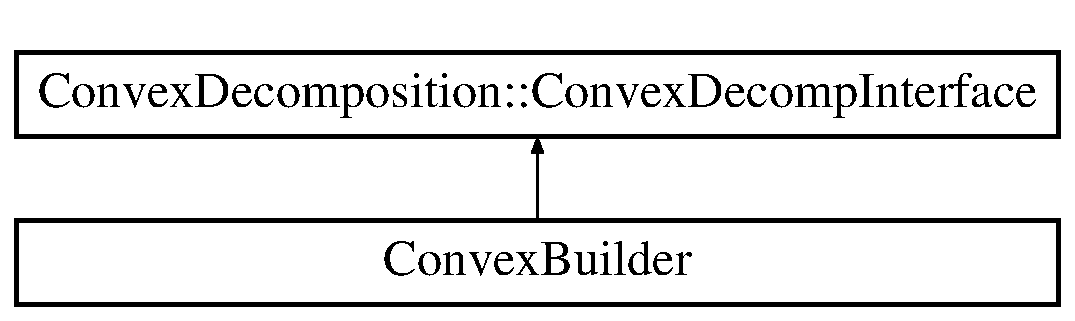
\includegraphics[height=2.000000cm]{class_convex_builder}
\end{center}
\end{figure}
\subsection*{Public Member Functions}
\begin{DoxyCompactItemize}
\item 
\hypertarget{class_convex_builder_a6f3cce36ddd0fa83dc8513e551ca954c}{{\bfseries Convex\-Builder} (\hyperlink{class_convex_decomposition_1_1_convex_decomp_interface}{Convex\-Decomp\-Interface} $\ast$callback)}\label{class_convex_builder_a6f3cce36ddd0fa83dc8513e551ca954c}

\item 
\hypertarget{class_convex_builder_a9203aa9ff35017024a611f48f3f3437b}{bool {\bfseries is\-Duplicate} (unsigned int i1, unsigned int i2, unsigned int i3, unsigned int ci1, unsigned int ci2, unsigned int ci3)}\label{class_convex_builder_a9203aa9ff35017024a611f48f3f3437b}

\item 
\hypertarget{class_convex_builder_ae2aada85346557d8780fcf35a0a13d0f}{void {\bfseries get\-Mesh} (const \hyperlink{class_convex_decomposition_1_1_convex_result}{Convex\-Result} \&cr, Vertex\-Lookup vc, Uint\-Vector \&indices)}\label{class_convex_builder_ae2aada85346557d8780fcf35a0a13d0f}

\item 
\hypertarget{class_convex_builder_afe09317380f052023cc33a44c8ad1afc}{\hyperlink{class_c_hull}{C\-Hull} $\ast$ {\bfseries can\-Merge} (\hyperlink{class_c_hull}{C\-Hull} $\ast$a, \hyperlink{class_c_hull}{C\-Hull} $\ast$b)}\label{class_convex_builder_afe09317380f052023cc33a44c8ad1afc}

\item 
\hypertarget{class_convex_builder_aa3310983f122da014be579a2c90507bc}{bool {\bfseries combine\-Hulls} (void)}\label{class_convex_builder_aa3310983f122da014be579a2c90507bc}

\item 
\hypertarget{class_convex_builder_aa60b2d47867847a1df4d1c8adf9e4dc1}{unsigned int {\bfseries process} (const \hyperlink{class_convex_decomposition_1_1_decomp_desc}{Decomp\-Desc} \&desc)}\label{class_convex_builder_aa60b2d47867847a1df4d1c8adf9e4dc1}

\item 
\hypertarget{class_convex_builder_a0d4761811c1aba03501f99c7fd3ac60b}{virtual void {\bfseries Convex\-Debug\-Tri} (const float $\ast$p1, const float $\ast$p2, const float $\ast$p3, unsigned int color)}\label{class_convex_builder_a0d4761811c1aba03501f99c7fd3ac60b}

\item 
\hypertarget{class_convex_builder_afb3bd186b8c5474987a8802fa3862207}{virtual void {\bfseries Convex\-Debug\-O\-B\-B} (const float $\ast$sides, const float $\ast$matrix, unsigned int color)}\label{class_convex_builder_afb3bd186b8c5474987a8802fa3862207}

\item 
\hypertarget{class_convex_builder_a27c203170b0517f2cafa230e668bfb53}{virtual void {\bfseries Convex\-Debug\-Point} (const float $\ast$p, float dist, unsigned int color)}\label{class_convex_builder_a27c203170b0517f2cafa230e668bfb53}

\item 
\hypertarget{class_convex_builder_ae70b8ed34b425867f6bd8fb0a85d63fa}{virtual void {\bfseries Convex\-Debug\-Bound} (const float $\ast$bmin, const float $\ast$bmax, unsigned int color)}\label{class_convex_builder_ae70b8ed34b425867f6bd8fb0a85d63fa}

\item 
\hypertarget{class_convex_builder_aa5ebbc3fb58777ff67f38900d54c2471}{virtual void {\bfseries Convex\-Decomp\-Result} (\hyperlink{class_convex_decomposition_1_1_convex_result}{Convex\-Result} \&result)}\label{class_convex_builder_aa5ebbc3fb58777ff67f38900d54c2471}

\item 
\hypertarget{class_convex_builder_a0bc79e8799a0c7daf3647b906e56a8c6}{void {\bfseries sort\-Chulls} (C\-Hull\-Vector \&hulls)}\label{class_convex_builder_a0bc79e8799a0c7daf3647b906e56a8c6}

\end{DoxyCompactItemize}
\subsection*{Public Attributes}
\begin{DoxyCompactItemize}
\item 
\hypertarget{class_convex_builder_a3afe639e250fe275559683d53d64cf8d}{C\-Hull\-Vector {\bfseries m\-Chulls}}\label{class_convex_builder_a3afe639e250fe275559683d53d64cf8d}

\item 
\hypertarget{class_convex_builder_a1f6f37473a9fe6abd1ea82d07d077a94}{\hyperlink{class_convex_decomposition_1_1_convex_decomp_interface}{Convex\-Decomp\-Interface} $\ast$ {\bfseries m\-Callback}}\label{class_convex_builder_a1f6f37473a9fe6abd1ea82d07d077a94}

\end{DoxyCompactItemize}


The documentation for this class was generated from the following files\-:\begin{DoxyCompactItemize}
\item 
A\-:/\-I\-T/\-Git\-Hub/\-I\-C\-T312/source/ogregraphics/Convex\-Builder.\-h\item 
A\-:/\-I\-T/\-Git\-Hub/\-I\-C\-T312/source/ogregraphics/Convex\-Builder.\-cpp\end{DoxyCompactItemize}

\hypertarget{class_convex_decomposition_1_1_convex_decomp_interface}{\section{Convex\-Decomposition\-:\-:Convex\-Decomp\-Interface Class Reference}
\label{class_convex_decomposition_1_1_convex_decomp_interface}\index{Convex\-Decomposition\-::\-Convex\-Decomp\-Interface@{Convex\-Decomposition\-::\-Convex\-Decomp\-Interface}}
}
Inheritance diagram for Convex\-Decomposition\-:\-:Convex\-Decomp\-Interface\-:\begin{figure}[H]
\begin{center}
\leavevmode
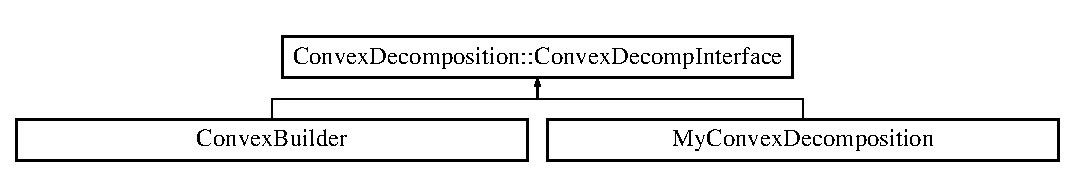
\includegraphics[height=1.931034cm]{class_convex_decomposition_1_1_convex_decomp_interface}
\end{center}
\end{figure}
\subsection*{Public Member Functions}
\begin{DoxyCompactItemize}
\item 
\hypertarget{class_convex_decomposition_1_1_convex_decomp_interface_ade260062de37fce5e72918240bdf7750}{virtual void {\bfseries Convex\-Debug\-Tri} (const float $\ast$p1, const float $\ast$p2, const float $\ast$p3, unsigned int color)}\label{class_convex_decomposition_1_1_convex_decomp_interface_ade260062de37fce5e72918240bdf7750}

\item 
\hypertarget{class_convex_decomposition_1_1_convex_decomp_interface_a4eb2606379b4d7cea0b8122dfbd17a7b}{virtual void {\bfseries Convex\-Debug\-Point} (const float $\ast$p, float dist, unsigned int color)}\label{class_convex_decomposition_1_1_convex_decomp_interface_a4eb2606379b4d7cea0b8122dfbd17a7b}

\item 
\hypertarget{class_convex_decomposition_1_1_convex_decomp_interface_a57ef84132a1c95862f543eb249f96d77}{virtual void {\bfseries Convex\-Debug\-Bound} (const float $\ast$bmin, const float $\ast$bmax, unsigned int color)}\label{class_convex_decomposition_1_1_convex_decomp_interface_a57ef84132a1c95862f543eb249f96d77}

\item 
\hypertarget{class_convex_decomposition_1_1_convex_decomp_interface_a3ae71f8a41bdffd2e0ad7bba985fc46a}{virtual void {\bfseries Convex\-Debug\-O\-B\-B} (const float $\ast$sides, const float $\ast$matrix, unsigned int color)}\label{class_convex_decomposition_1_1_convex_decomp_interface_a3ae71f8a41bdffd2e0ad7bba985fc46a}

\item 
\hypertarget{class_convex_decomposition_1_1_convex_decomp_interface_a23b944ece0d378c5ced4eed6e66ae14a}{virtual void {\bfseries Convex\-Decomp\-Result} (\hyperlink{class_convex_decomposition_1_1_convex_result}{Convex\-Result} \&result)=0}\label{class_convex_decomposition_1_1_convex_decomp_interface_a23b944ece0d378c5ced4eed6e66ae14a}

\end{DoxyCompactItemize}


The documentation for this class was generated from the following file\-:\begin{DoxyCompactItemize}
\item 
A\-:/\-I\-T/\-Git\-Hub/\-I\-C\-T312/source/ogregraphics/\-Extras/Convex\-Decomposition.\-h\end{DoxyCompactItemize}

\hypertarget{class_convex_decomposition_1_1_convex_result}{\section{Convex\-Decomposition\-:\-:Convex\-Result Class Reference}
\label{class_convex_decomposition_1_1_convex_result}\index{Convex\-Decomposition\-::\-Convex\-Result@{Convex\-Decomposition\-::\-Convex\-Result}}
}
\subsection*{Public Member Functions}
\begin{DoxyCompactItemize}
\item 
\hypertarget{class_convex_decomposition_1_1_convex_result_af2d96bc26f1bc45b0ccc21052ed18c67}{{\bfseries Convex\-Result} (unsigned int hvcount, const float $\ast$hvertices, unsigned int htcount, const unsigned int $\ast$hindices)}\label{class_convex_decomposition_1_1_convex_result_af2d96bc26f1bc45b0ccc21052ed18c67}

\item 
\hypertarget{class_convex_decomposition_1_1_convex_result_afc7a0d697c1050875a37986d71cee344}{{\bfseries Convex\-Result} (const \hyperlink{class_convex_decomposition_1_1_convex_result}{Convex\-Result} \&r)}\label{class_convex_decomposition_1_1_convex_result_afc7a0d697c1050875a37986d71cee344}

\end{DoxyCompactItemize}
\subsection*{Public Attributes}
\begin{DoxyCompactItemize}
\item 
\hypertarget{class_convex_decomposition_1_1_convex_result_a0deb6d4bf255da267bf01d82100bef80}{unsigned int {\bfseries m\-Hull\-Vcount}}\label{class_convex_decomposition_1_1_convex_result_a0deb6d4bf255da267bf01d82100bef80}

\item 
\hypertarget{class_convex_decomposition_1_1_convex_result_a798a0276ecea7cd6f155bc26c51bf54e}{float $\ast$ {\bfseries m\-Hull\-Vertices}}\label{class_convex_decomposition_1_1_convex_result_a798a0276ecea7cd6f155bc26c51bf54e}

\item 
\hypertarget{class_convex_decomposition_1_1_convex_result_af2c64d2cd03f9defe43ffae315057f67}{unsigned int {\bfseries m\-Hull\-Tcount}}\label{class_convex_decomposition_1_1_convex_result_af2c64d2cd03f9defe43ffae315057f67}

\item 
\hypertarget{class_convex_decomposition_1_1_convex_result_ae84d2842c2889afdfd4ad95a6b812ce6}{unsigned int $\ast$ {\bfseries m\-Hull\-Indices}}\label{class_convex_decomposition_1_1_convex_result_ae84d2842c2889afdfd4ad95a6b812ce6}

\item 
\hypertarget{class_convex_decomposition_1_1_convex_result_a80a3798574b15ac887ef6e11844b256c}{float {\bfseries m\-Hull\-Volume}}\label{class_convex_decomposition_1_1_convex_result_a80a3798574b15ac887ef6e11844b256c}

\item 
\hypertarget{class_convex_decomposition_1_1_convex_result_a2a8a970091b794a2b53ff1d983800d05}{float {\bfseries m\-O\-B\-B\-Sides} \mbox{[}3\mbox{]}}\label{class_convex_decomposition_1_1_convex_result_a2a8a970091b794a2b53ff1d983800d05}

\item 
\hypertarget{class_convex_decomposition_1_1_convex_result_aaa28d7790a0cddec9453cbf4c60f0dd8}{float {\bfseries m\-O\-B\-B\-Center} \mbox{[}3\mbox{]}}\label{class_convex_decomposition_1_1_convex_result_aaa28d7790a0cddec9453cbf4c60f0dd8}

\item 
\hypertarget{class_convex_decomposition_1_1_convex_result_a6c63b72bbbc8484204a28d29c81e4f89}{float {\bfseries m\-O\-B\-B\-Orientation} \mbox{[}4\mbox{]}}\label{class_convex_decomposition_1_1_convex_result_a6c63b72bbbc8484204a28d29c81e4f89}

\item 
\hypertarget{class_convex_decomposition_1_1_convex_result_ab47652a96740e87a4429fc814b8a8514}{float {\bfseries m\-O\-B\-B\-Transform} \mbox{[}16\mbox{]}}\label{class_convex_decomposition_1_1_convex_result_ab47652a96740e87a4429fc814b8a8514}

\item 
\hypertarget{class_convex_decomposition_1_1_convex_result_a853b2f5ff4672523fd757b087e7d4966}{float {\bfseries m\-O\-B\-B\-Volume}}\label{class_convex_decomposition_1_1_convex_result_a853b2f5ff4672523fd757b087e7d4966}

\item 
\hypertarget{class_convex_decomposition_1_1_convex_result_ab06db274a09247f65760cd634b535445}{float {\bfseries m\-Sphere\-Radius}}\label{class_convex_decomposition_1_1_convex_result_ab06db274a09247f65760cd634b535445}

\item 
\hypertarget{class_convex_decomposition_1_1_convex_result_ac25b672d8760308c3bb7cbadec3551a3}{float {\bfseries m\-Sphere\-Center} \mbox{[}3\mbox{]}}\label{class_convex_decomposition_1_1_convex_result_ac25b672d8760308c3bb7cbadec3551a3}

\item 
\hypertarget{class_convex_decomposition_1_1_convex_result_a04711a2ef01d11c920758058ba491357}{float {\bfseries m\-Sphere\-Volume}}\label{class_convex_decomposition_1_1_convex_result_a04711a2ef01d11c920758058ba491357}

\end{DoxyCompactItemize}


The documentation for this class was generated from the following file\-:\begin{DoxyCompactItemize}
\item 
A\-:/\-I\-T/\-Git\-Hub/\-I\-C\-T312/source/ogregraphics/\-Extras/Convex\-Decomposition.\-h\end{DoxyCompactItemize}

\hypertarget{class_debug_drawer}{\section{Debug\-Drawer Class Reference}
\label{class_debug_drawer}\index{Debug\-Drawer@{Debug\-Drawer}}
}
Inheritance diagram for Debug\-Drawer\-:\begin{figure}[H]
\begin{center}
\leavevmode
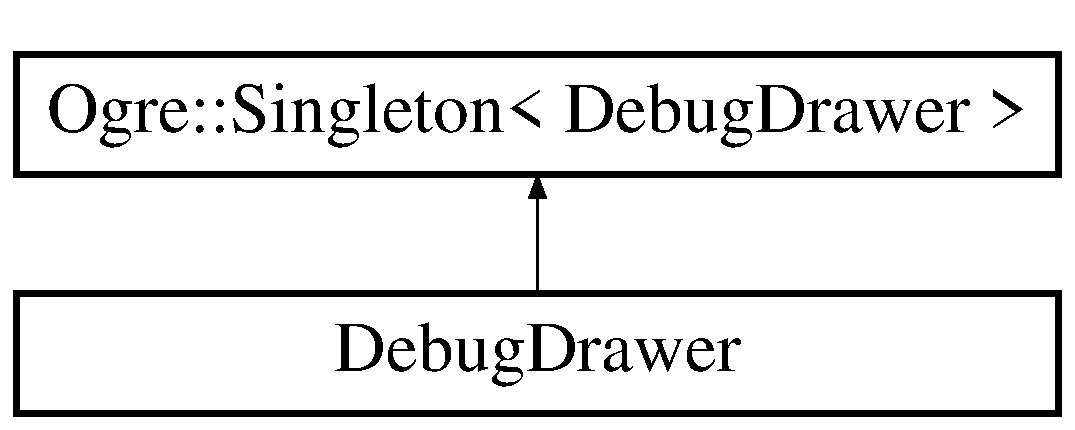
\includegraphics[height=2.000000cm]{class_debug_drawer}
\end{center}
\end{figure}
\subsection*{Public Member Functions}
\begin{DoxyCompactItemize}
\item 
\hypertarget{class_debug_drawer_a7cb360171f2209e271dbdb353a57da29}{{\bfseries Debug\-Drawer} (Ogre\-::\-Scene\-Manager $\ast$\-\_\-scene\-Manager, float \-\_\-fill\-Alpha)}\label{class_debug_drawer_a7cb360171f2209e271dbdb353a57da29}

\item 
\hypertarget{class_debug_drawer_a4c94a09fac8cc826ae569dc0b735470e}{void {\bfseries build} ()}\label{class_debug_drawer_a4c94a09fac8cc826ae569dc0b735470e}

\item 
\hypertarget{class_debug_drawer_a7fd058d2116a2f0ef0ca54ee1d07afc0}{void {\bfseries set\-Ico\-Sphere\-Recursion\-Level} (int recursion\-Level)}\label{class_debug_drawer_a7fd058d2116a2f0ef0ca54ee1d07afc0}

\item 
\hypertarget{class_debug_drawer_aefcd3e33bc435c9107bbcf502224d6a6}{void {\bfseries draw\-Line} (const Ogre\-::\-Vector3 \&start, const Ogre\-::\-Vector3 \&end, const Ogre\-::\-Colour\-Value \&colour)}\label{class_debug_drawer_aefcd3e33bc435c9107bbcf502224d6a6}

\item 
\hypertarget{class_debug_drawer_a1eae1b0a9536d8f1f6af2d182beeb1c6}{void {\bfseries draw\-Circle} (const Ogre\-::\-Vector3 \&centre, float radius, int segments\-Count, const Ogre\-::\-Colour\-Value \&colour, bool is\-Filled=false)}\label{class_debug_drawer_a1eae1b0a9536d8f1f6af2d182beeb1c6}

\item 
\hypertarget{class_debug_drawer_aa582fdbb8678c3f183be8d08c3fe33ad}{void {\bfseries draw\-Cylinder} (const Ogre\-::\-Vector3 \&centre, float radius, int segments\-Count, float height, const Ogre\-::\-Colour\-Value \&colour, bool is\-Filled=false)}\label{class_debug_drawer_aa582fdbb8678c3f183be8d08c3fe33ad}

\item 
\hypertarget{class_debug_drawer_ab950e2c862842897cfdc22726a1469f1}{void {\bfseries draw\-Quad} (const Ogre\-::\-Vector3 $\ast$vertices, const Ogre\-::\-Colour\-Value \&colour, bool is\-Filled=false)}\label{class_debug_drawer_ab950e2c862842897cfdc22726a1469f1}

\item 
\hypertarget{class_debug_drawer_a50b17ab0d65f002d22cce2a3dfbe4f78}{void {\bfseries draw\-Cuboid} (const Ogre\-::\-Vector3 $\ast$vertices, const Ogre\-::\-Colour\-Value \&colour, bool is\-Filled=false)}\label{class_debug_drawer_a50b17ab0d65f002d22cce2a3dfbe4f78}

\item 
\hypertarget{class_debug_drawer_ab40cd48a32e8577cf9eed6197c3f1929}{void {\bfseries draw\-Sphere} (const Ogre\-::\-Vector3 \&centre, float radius, const Ogre\-::\-Colour\-Value \&colour, bool is\-Filled=false)}\label{class_debug_drawer_ab40cd48a32e8577cf9eed6197c3f1929}

\item 
\hypertarget{class_debug_drawer_aaa8da061a80b0aceab062dd9217c75e5}{void {\bfseries draw\-Tetrahedron} (const Ogre\-::\-Vector3 \&centre, float scale, const Ogre\-::\-Colour\-Value \&colour, bool is\-Filled=false)}\label{class_debug_drawer_aaa8da061a80b0aceab062dd9217c75e5}

\item 
\hypertarget{class_debug_drawer_a01792a65e18f16a8eab3b5bb81095467}{bool {\bfseries get\-Enabled} ()}\label{class_debug_drawer_a01792a65e18f16a8eab3b5bb81095467}

\item 
\hypertarget{class_debug_drawer_a345e07f6bf1c6f159f09907dcfe1c07f}{void {\bfseries set\-Enabled} (bool \-\_\-is\-Enabled)}\label{class_debug_drawer_a345e07f6bf1c6f159f09907dcfe1c07f}

\item 
\hypertarget{class_debug_drawer_ac482f4d2f6be3b5037988594f1fd41eb}{void {\bfseries switch\-Enabled} ()}\label{class_debug_drawer_ac482f4d2f6be3b5037988594f1fd41eb}

\item 
\hypertarget{class_debug_drawer_a7a10010490fdeba658aad0b040750e24}{void {\bfseries clear} ()}\label{class_debug_drawer_a7a10010490fdeba658aad0b040750e24}

\end{DoxyCompactItemize}
\subsection*{Static Public Member Functions}
\begin{DoxyCompactItemize}
\item 
\hypertarget{class_debug_drawer_a0a8f7a51871ed9e45add15e03379c7bd}{static \hyperlink{class_debug_drawer}{Debug\-Drawer} \& {\bfseries get\-Singleton} (void)}\label{class_debug_drawer_a0a8f7a51871ed9e45add15e03379c7bd}

\item 
\hypertarget{class_debug_drawer_a71ac854db9068c93c7e08a02033c7f3f}{static \hyperlink{class_debug_drawer}{Debug\-Drawer} $\ast$ {\bfseries get\-Singleton\-Ptr} (void)}\label{class_debug_drawer_a71ac854db9068c93c7e08a02033c7f3f}

\end{DoxyCompactItemize}


The documentation for this class was generated from the following files\-:\begin{DoxyCompactItemize}
\item 
A\-:/\-I\-T/\-Git\-Hub/\-I\-C\-T312/source/ogregraphics/Debug\-Drawer.\-h\item 
A\-:/\-I\-T/\-Git\-Hub/\-I\-C\-T312/source/ogregraphics/Debug\-Drawer.\-cpp\end{DoxyCompactItemize}

\hypertarget{class_convex_decomposition_1_1_decomp_desc}{\section{Convex\-Decomposition\-:\-:Decomp\-Desc Class Reference}
\label{class_convex_decomposition_1_1_decomp_desc}\index{Convex\-Decomposition\-::\-Decomp\-Desc@{Convex\-Decomposition\-::\-Decomp\-Desc}}
}
\subsection*{Public Attributes}
\begin{DoxyCompactItemize}
\item 
\hypertarget{class_convex_decomposition_1_1_decomp_desc_ad29b91a963df41cefa7235201323f3b4}{unsigned int {\bfseries m\-Vcount}}\label{class_convex_decomposition_1_1_decomp_desc_ad29b91a963df41cefa7235201323f3b4}

\item 
\hypertarget{class_convex_decomposition_1_1_decomp_desc_a0f8347667402ee1c78be17a8e7e73e2b}{const float $\ast$ {\bfseries m\-Vertices}}\label{class_convex_decomposition_1_1_decomp_desc_a0f8347667402ee1c78be17a8e7e73e2b}

\item 
\hypertarget{class_convex_decomposition_1_1_decomp_desc_a96c4557cd6f3c0868cf231f152ed1fb4}{unsigned int {\bfseries m\-Tcount}}\label{class_convex_decomposition_1_1_decomp_desc_a96c4557cd6f3c0868cf231f152ed1fb4}

\item 
\hypertarget{class_convex_decomposition_1_1_decomp_desc_a030c95c09800d3cdcd03c7180450f4a4}{unsigned int $\ast$ {\bfseries m\-Indices}}\label{class_convex_decomposition_1_1_decomp_desc_a030c95c09800d3cdcd03c7180450f4a4}

\item 
\hypertarget{class_convex_decomposition_1_1_decomp_desc_ad4eddfbbbb168d591d351935dc56b3e4}{unsigned int {\bfseries m\-Depth}}\label{class_convex_decomposition_1_1_decomp_desc_ad4eddfbbbb168d591d351935dc56b3e4}

\item 
\hypertarget{class_convex_decomposition_1_1_decomp_desc_aeaeb0530e55390a315656ea93979be5b}{float {\bfseries m\-Cpercent}}\label{class_convex_decomposition_1_1_decomp_desc_aeaeb0530e55390a315656ea93979be5b}

\item 
\hypertarget{class_convex_decomposition_1_1_decomp_desc_a8a43f17357737275d5a002c494c8d36f}{float {\bfseries m\-Ppercent}}\label{class_convex_decomposition_1_1_decomp_desc_a8a43f17357737275d5a002c494c8d36f}

\item 
\hypertarget{class_convex_decomposition_1_1_decomp_desc_aebaa387f6e17beac565adf831b535dc0}{unsigned int {\bfseries m\-Max\-Vertices}}\label{class_convex_decomposition_1_1_decomp_desc_aebaa387f6e17beac565adf831b535dc0}

\item 
\hypertarget{class_convex_decomposition_1_1_decomp_desc_a60d16f6a176268ca4ddf940fd247015b}{float {\bfseries m\-Skin\-Width}}\label{class_convex_decomposition_1_1_decomp_desc_a60d16f6a176268ca4ddf940fd247015b}

\item 
\hypertarget{class_convex_decomposition_1_1_decomp_desc_aed8ce4212508ed98f8002e53372ccc84}{\hyperlink{class_convex_decomposition_1_1_convex_decomp_interface}{Convex\-Decomp\-Interface} $\ast$ {\bfseries m\-Callback}}\label{class_convex_decomposition_1_1_decomp_desc_aed8ce4212508ed98f8002e53372ccc84}

\end{DoxyCompactItemize}


The documentation for this class was generated from the following file\-:\begin{DoxyCompactItemize}
\item 
A\-:/\-I\-T/\-Git\-Hub/\-I\-C\-T312/source/ogregraphics/\-Extras/Convex\-Decomposition.\-h\end{DoxyCompactItemize}

\hypertarget{class_easy_going}{\section{Easy\-Going Class Reference}
\label{class_easy_going}\index{Easy\-Going@{Easy\-Going}}
}


Easy going.  




{\ttfamily \#include $<$Easy\-Going.\-h$>$}

Inheritance diagram for Easy\-Going\-:\begin{figure}[H]
\begin{center}
\leavevmode
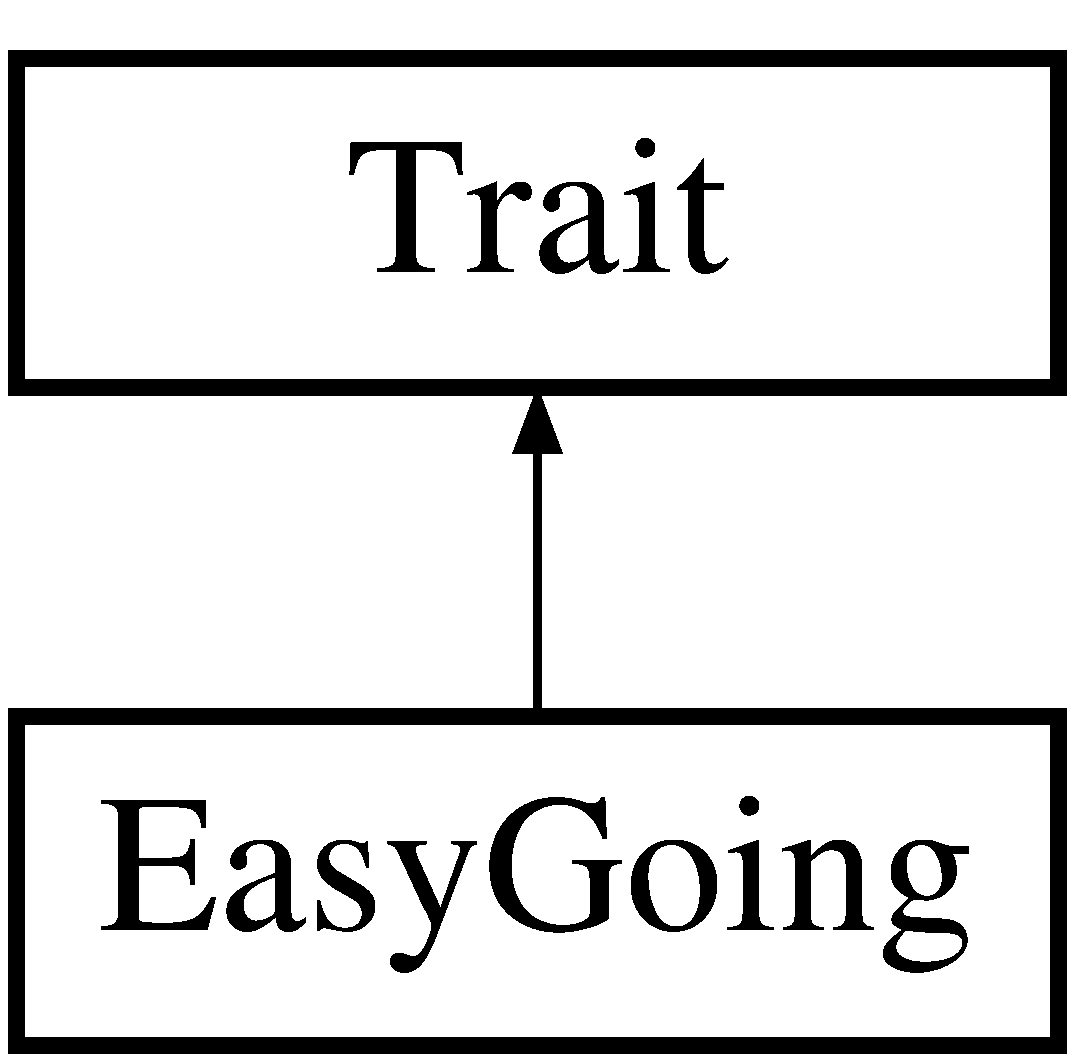
\includegraphics[height=2.000000cm]{class_easy_going}
\end{center}
\end{figure}
\subsection*{Public Member Functions}
\begin{DoxyCompactItemize}
\item 
\hyperlink{class_easy_going_abdfa649d6749ce01bbcad9d20e3ecd3d}{Easy\-Going} (void)
\begin{DoxyCompactList}\small\item\em Default constructor. \end{DoxyCompactList}\item 
\hyperlink{class_easy_going_a731112713c4053ab8485c3e4b2029fd4}{$\sim$\-Easy\-Going} (void)
\begin{DoxyCompactList}\small\item\em Destructor. \end{DoxyCompactList}\end{DoxyCompactItemize}


\subsection{Detailed Description}
Easy going. 

\begin{DoxyAuthor}{Author}
Hamish Carrier 
\end{DoxyAuthor}
\begin{DoxyDate}{Date}
10/11/2013 
\end{DoxyDate}


\subsection{Constructor \& Destructor Documentation}
\hypertarget{class_easy_going_abdfa649d6749ce01bbcad9d20e3ecd3d}{\index{Easy\-Going@{Easy\-Going}!Easy\-Going@{Easy\-Going}}
\index{Easy\-Going@{Easy\-Going}!EasyGoing@{Easy\-Going}}
\subsubsection[{Easy\-Going}]{\setlength{\rightskip}{0pt plus 5cm}Easy\-Going\-::\-Easy\-Going (
\begin{DoxyParamCaption}
\item[{void}]{}
\end{DoxyParamCaption}
)}}\label{class_easy_going_abdfa649d6749ce01bbcad9d20e3ecd3d}


Default constructor. 

\begin{DoxyAuthor}{Author}
Hamish Carrier 
\end{DoxyAuthor}
\begin{DoxyDate}{Date}
10/11/2013 
\end{DoxyDate}
\hypertarget{class_easy_going_a731112713c4053ab8485c3e4b2029fd4}{\index{Easy\-Going@{Easy\-Going}!$\sim$\-Easy\-Going@{$\sim$\-Easy\-Going}}
\index{$\sim$\-Easy\-Going@{$\sim$\-Easy\-Going}!EasyGoing@{Easy\-Going}}
\subsubsection[{$\sim$\-Easy\-Going}]{\setlength{\rightskip}{0pt plus 5cm}Easy\-Going\-::$\sim$\-Easy\-Going (
\begin{DoxyParamCaption}
\item[{void}]{}
\end{DoxyParamCaption}
)}}\label{class_easy_going_a731112713c4053ab8485c3e4b2029fd4}


Destructor. 

\begin{DoxyAuthor}{Author}
Hamish Carrier 
\end{DoxyAuthor}
\begin{DoxyDate}{Date}
10/11/2013 
\end{DoxyDate}


The documentation for this class was generated from the following files\-:\begin{DoxyCompactItemize}
\item 
A\-:/\-I\-T/\-Git\-Hub/\-I\-C\-T312/source/ogregraphics/\hyperlink{_easy_going_8h}{Easy\-Going.\-h}\item 
A\-:/\-I\-T/\-Git\-Hub/\-I\-C\-T312/source/ogregraphics/Easy\-Going.\-cpp\end{DoxyCompactItemize}

\hypertarget{class_emotion}{\section{Emotion Class Reference}
\label{class_emotion}\index{Emotion@{Emotion}}
}


\hyperlink{class_emotion}{Emotion}.  




{\ttfamily \#include $<$Emotion.\-h$>$}

Inheritance diagram for Emotion\-:\begin{figure}[H]
\begin{center}
\leavevmode
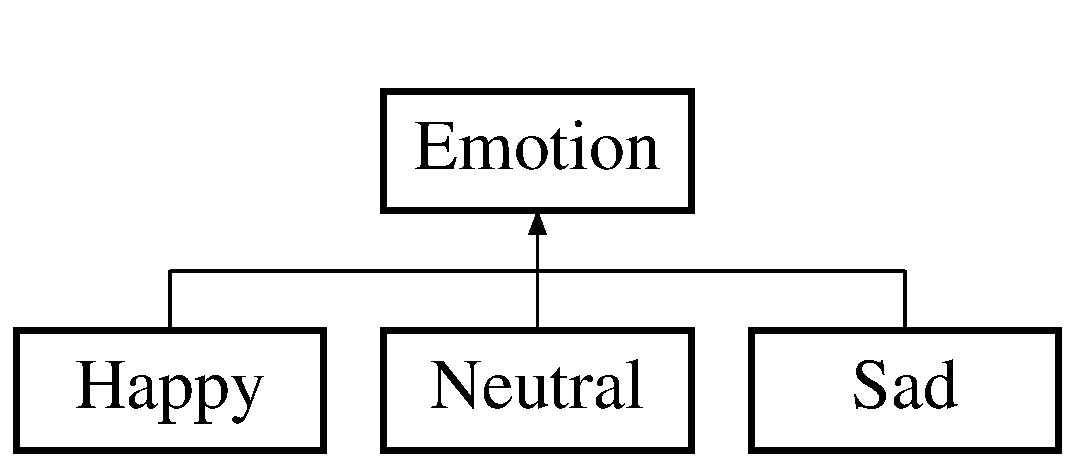
\includegraphics[height=2.000000cm]{class_emotion}
\end{center}
\end{figure}


\subsection{Detailed Description}
\hyperlink{class_emotion}{Emotion}. 

\begin{DoxyAuthor}{Author}
Hamish Carrier 
\end{DoxyAuthor}
\begin{DoxyDate}{Date}
10/11/2013 
\end{DoxyDate}


The documentation for this class was generated from the following file\-:\begin{DoxyCompactItemize}
\item 
A\-:/\-I\-T/\-Git\-Hub/\-I\-C\-T312/source/ogregraphics/\hyperlink{_emotion_8h}{Emotion.\-h}\end{DoxyCompactItemize}

\hypertarget{class_emotion_manager}{\section{Emotion\-Manager Class Reference}
\label{class_emotion_manager}\index{Emotion\-Manager@{Emotion\-Manager}}
}


Manager for emotions.  




{\ttfamily \#include $<$Emotion\-Manager.\-h$>$}

\subsection*{Public Member Functions}
\begin{DoxyCompactItemize}
\item 
\hyperlink{class_emotion}{Emotion} $\ast$ \hyperlink{class_emotion_manager_a812664d891d04508b147fd7c6a1e9072}{Fetch\-Emotion} (Enum\-Space\-::\-Emotion\-Types Desired\-Emotion)
\begin{DoxyCompactList}\small\item\em Fetches an emotion. \end{DoxyCompactList}\end{DoxyCompactItemize}
\subsection*{Static Public Member Functions}
\begin{DoxyCompactItemize}
\item 
static \hyperlink{class_emotion_manager}{Emotion\-Manager} $\ast$ \hyperlink{class_emotion_manager_ade6b3cfab0145c7dff38884d85670b92}{Get\-Instance} ()
\begin{DoxyCompactList}\small\item\em Gets the instance. \end{DoxyCompactList}\end{DoxyCompactItemize}


\subsection{Detailed Description}
Manager for emotions. 

\begin{DoxyAuthor}{Author}
Hamish Carrier 
\end{DoxyAuthor}
\begin{DoxyDate}{Date}
10/11/2013 
\end{DoxyDate}


\subsection{Member Function Documentation}
\hypertarget{class_emotion_manager_a812664d891d04508b147fd7c6a1e9072}{\index{Emotion\-Manager@{Emotion\-Manager}!Fetch\-Emotion@{Fetch\-Emotion}}
\index{Fetch\-Emotion@{Fetch\-Emotion}!EmotionManager@{Emotion\-Manager}}
\subsubsection[{Fetch\-Emotion}]{\setlength{\rightskip}{0pt plus 5cm}{\bf Emotion} $\ast$ Emotion\-Manager\-::\-Fetch\-Emotion (
\begin{DoxyParamCaption}
\item[{Enum\-Space\-::\-Emotion\-Types}]{Desired\-Emotion}
\end{DoxyParamCaption}
)}}\label{class_emotion_manager_a812664d891d04508b147fd7c6a1e9072}


Fetches an emotion. 

\begin{DoxyAuthor}{Author}
Hamish Carrier 
\end{DoxyAuthor}
\begin{DoxyDate}{Date}
10/11/2013
\end{DoxyDate}

\begin{DoxyParams}{Parameters}
{\em Desired\-Emotion} & The desired emotion.\\
\hline
\end{DoxyParams}
\begin{DoxyReturn}{Returns}
null if it fails, else the emotion. 
\end{DoxyReturn}
\hypertarget{class_emotion_manager_ade6b3cfab0145c7dff38884d85670b92}{\index{Emotion\-Manager@{Emotion\-Manager}!Get\-Instance@{Get\-Instance}}
\index{Get\-Instance@{Get\-Instance}!EmotionManager@{Emotion\-Manager}}
\subsubsection[{Get\-Instance}]{\setlength{\rightskip}{0pt plus 5cm}static {\bf Emotion\-Manager} $\ast$ Emotion\-Manager\-::\-Get\-Instance (
\begin{DoxyParamCaption}
{}
\end{DoxyParamCaption}
)\hspace{0.3cm}{\ttfamily [static]}}}\label{class_emotion_manager_ade6b3cfab0145c7dff38884d85670b92}


Gets the instance. 

\begin{DoxyAuthor}{Author}
Hamish Carrier 
\end{DoxyAuthor}
\begin{DoxyDate}{Date}
10/11/2013
\end{DoxyDate}
\begin{DoxyReturn}{Returns}
null if it fails, else the instance. 
\end{DoxyReturn}


The documentation for this class was generated from the following files\-:\begin{DoxyCompactItemize}
\item 
A\-:/\-I\-T/\-Git\-Hub/\-I\-C\-T312/source/ogregraphics/\hyperlink{_emotion_manager_8h}{Emotion\-Manager.\-h}\item 
A\-:/\-I\-T/\-Git\-Hub/\-I\-C\-T312/source/ogregraphics/Emotion\-Manager.\-cpp\end{DoxyCompactItemize}

\hypertarget{class_scenes_1_1_exit_scene}{\section{Scenes\-:\-:Exit\-Scene Class Reference}
\label{class_scenes_1_1_exit_scene}\index{Scenes\-::\-Exit\-Scene@{Scenes\-::\-Exit\-Scene}}
}
Inheritance diagram for Scenes\-:\-:Exit\-Scene\-:\begin{figure}[H]
\begin{center}
\leavevmode
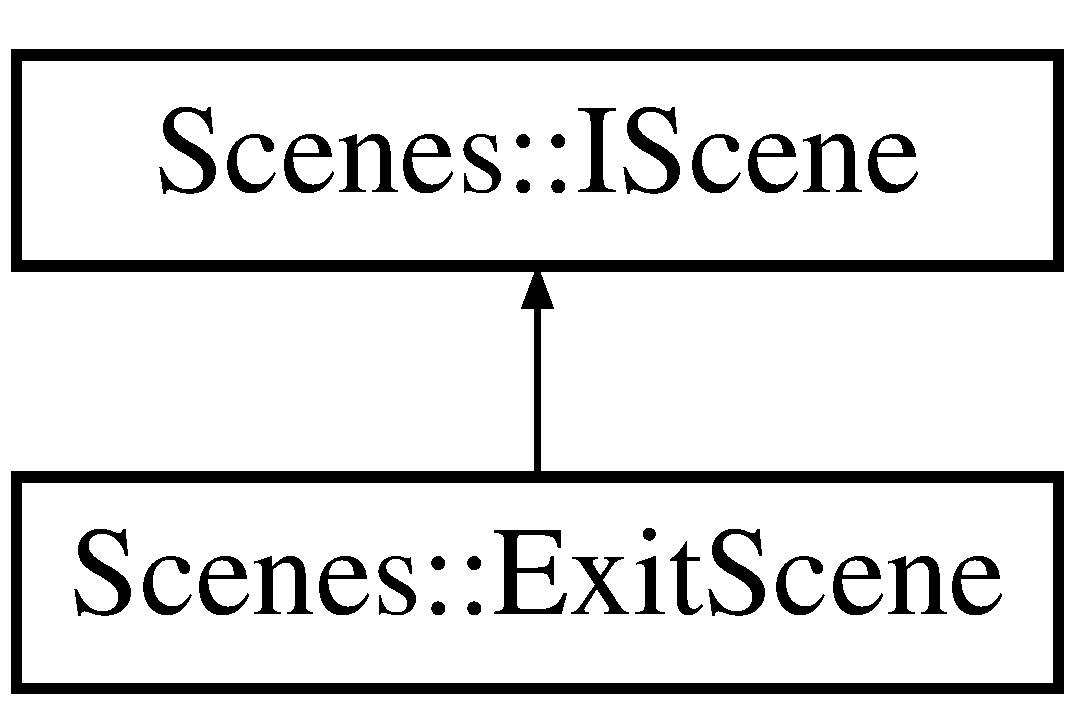
\includegraphics[height=2.000000cm]{class_scenes_1_1_exit_scene}
\end{center}
\end{figure}
\subsection*{Public Member Functions}
\begin{DoxyCompactItemize}
\item 
\hypertarget{class_scenes_1_1_exit_scene_ad39e5fca23387683608bf0c390434563}{virtual void \hyperlink{class_scenes_1_1_exit_scene_ad39e5fca23387683608bf0c390434563}{initialise} ()}\label{class_scenes_1_1_exit_scene_ad39e5fca23387683608bf0c390434563}

\begin{DoxyCompactList}\small\item\em Initialises the scene. \end{DoxyCompactList}\item 
virtual void \hyperlink{class_scenes_1_1_exit_scene_ab252f553afc98976f67a0e2c330caed4}{update} (float delta\-Time)
\begin{DoxyCompactList}\small\item\em Updates the scene given the change in time from one frame to another. \end{DoxyCompactList}\item 
\hypertarget{class_scenes_1_1_exit_scene_ad43b8fa0711409e3e887ab61d17b758e}{virtual void \hyperlink{class_scenes_1_1_exit_scene_ad43b8fa0711409e3e887ab61d17b758e}{on\-Exit} ()}\label{class_scenes_1_1_exit_scene_ad43b8fa0711409e3e887ab61d17b758e}

\begin{DoxyCompactList}\small\item\em Called upon the scene being closed. \end{DoxyCompactList}\end{DoxyCompactItemize}


\subsection{Member Function Documentation}
\hypertarget{class_scenes_1_1_exit_scene_ab252f553afc98976f67a0e2c330caed4}{\index{Scenes\-::\-Exit\-Scene@{Scenes\-::\-Exit\-Scene}!update@{update}}
\index{update@{update}!Scenes::ExitScene@{Scenes\-::\-Exit\-Scene}}
\subsubsection[{update}]{\setlength{\rightskip}{0pt plus 5cm}void Exit\-Scene\-::update (
\begin{DoxyParamCaption}
\item[{float}]{delta\-Time}
\end{DoxyParamCaption}
)\hspace{0.3cm}{\ttfamily [virtual]}}}\label{class_scenes_1_1_exit_scene_ab252f553afc98976f67a0e2c330caed4}


Updates the scene given the change in time from one frame to another. 


\begin{DoxyParams}{Parameters}
{\em delta\-Time} & The change in time from one frame to another. \\
\hline
\end{DoxyParams}


Reimplemented from \hyperlink{class_scenes_1_1_i_scene_acb97c42a9a93ce1b3d0b800bda680935}{Scenes\-::\-I\-Scene}.



The documentation for this class was generated from the following files\-:\begin{DoxyCompactItemize}
\item 
A\-:/\-I\-T/\-Git\-Hub/\-I\-C\-T312/source/ogregraphics/Exit\-Scene.\-h\item 
A\-:/\-I\-T/\-Git\-Hub/\-I\-C\-T312/source/ogregraphics/Exit\-Scene.\-cpp\end{DoxyCompactItemize}

\hypertarget{class_graphics_1_1_frame_listener}{\section{Graphics\-:\-:Frame\-Listener Class Reference}
\label{class_graphics_1_1_frame_listener}\index{Graphics\-::\-Frame\-Listener@{Graphics\-::\-Frame\-Listener}}
}


Frame listener.  




{\ttfamily \#include $<$Frame\-Listener.\-h$>$}

Inheritance diagram for Graphics\-:\-:Frame\-Listener\-:\begin{figure}[H]
\begin{center}
\leavevmode
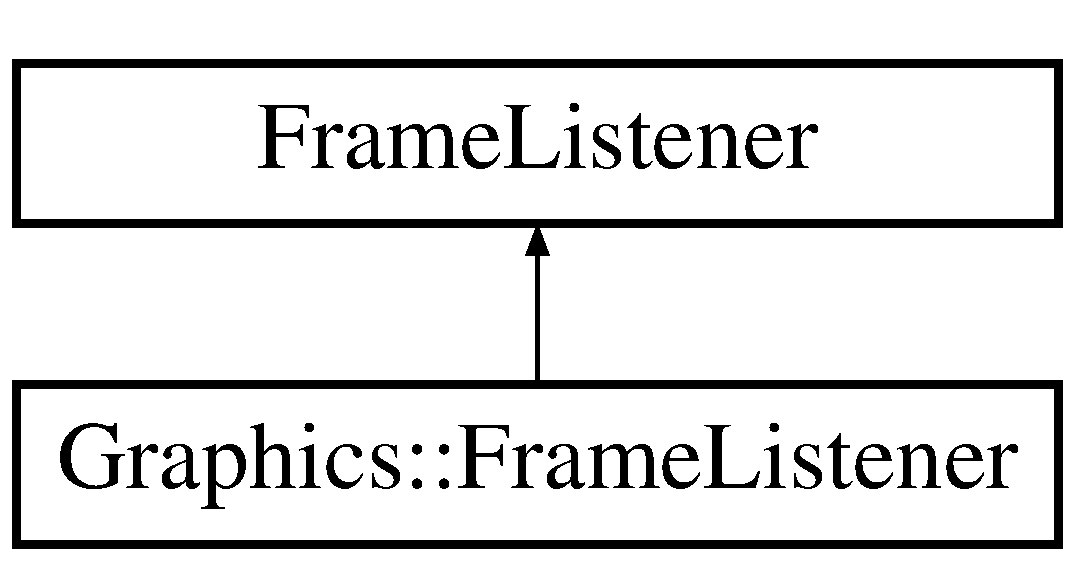
\includegraphics[height=2.000000cm]{class_graphics_1_1_frame_listener}
\end{center}
\end{figure}
\subsection*{Public Member Functions}
\begin{DoxyCompactItemize}
\item 
\hyperlink{class_graphics_1_1_frame_listener_afebcc6a4dc070985a77fb2182119ca98}{Frame\-Listener} (Ogre\-::\-Scene\-Manager $\ast$scene\-Manager)
\begin{DoxyCompactList}\small\item\em Constructor. \end{DoxyCompactList}\item 
\hypertarget{class_graphics_1_1_frame_listener_a84ee3a42ba673ac10825b25abcef248a}{\hyperlink{class_graphics_1_1_frame_listener_a84ee3a42ba673ac10825b25abcef248a}{$\sim$\-Frame\-Listener} ()}\label{class_graphics_1_1_frame_listener_a84ee3a42ba673ac10825b25abcef248a}

\begin{DoxyCompactList}\small\item\em Destructor. \end{DoxyCompactList}\item 
virtual bool \hyperlink{class_graphics_1_1_frame_listener_aa790d32da6634e931c35b69f779fd42b}{frame\-Started} (const Ogre\-::\-Frame\-Event \&evt)
\begin{DoxyCompactList}\small\item\em Frame started. \end{DoxyCompactList}\item 
virtual bool \hyperlink{class_graphics_1_1_frame_listener_a3aa34e5431cef9ad1d429790914eed60}{frame\-Ended} (const Ogre\-::\-Frame\-Event \&evt)
\begin{DoxyCompactList}\small\item\em Frame ended. \end{DoxyCompactList}\item 
virtual bool \hyperlink{class_graphics_1_1_frame_listener_a1ea51ffd9cfb64758c0bde5d0036a510}{frame\-Rendering\-Queued} (const Ogre\-::\-Frame\-Event \&evt)
\begin{DoxyCompactList}\small\item\em Frame rendering queued. \end{DoxyCompactList}\item 
float \hyperlink{class_graphics_1_1_frame_listener_a2f8f5e7b39811078ec7d735233e41d74}{get\-Delta\-Time} () const 
\begin{DoxyCompactList}\small\item\em Gets delta time. \end{DoxyCompactList}\end{DoxyCompactItemize}


\subsection{Detailed Description}
Frame listener. 

\subsection{Constructor \& Destructor Documentation}
\hypertarget{class_graphics_1_1_frame_listener_afebcc6a4dc070985a77fb2182119ca98}{\index{Graphics\-::\-Frame\-Listener@{Graphics\-::\-Frame\-Listener}!Frame\-Listener@{Frame\-Listener}}
\index{Frame\-Listener@{Frame\-Listener}!Graphics::FrameListener@{Graphics\-::\-Frame\-Listener}}
\subsubsection[{Frame\-Listener}]{\setlength{\rightskip}{0pt plus 5cm}Graphics\-::\-Frame\-Listener\-::\-Frame\-Listener (
\begin{DoxyParamCaption}
\item[{Ogre\-::\-Scene\-Manager $\ast$}]{scene\-Manager}
\end{DoxyParamCaption}
)}}\label{class_graphics_1_1_frame_listener_afebcc6a4dc070985a77fb2182119ca98}


Constructor. 


\begin{DoxyParams}[1]{Parameters}
\mbox{\tt in,out}  & {\em scene\-Manager} & If non-\/null, manager for scene. \\
\hline
\end{DoxyParams}


\subsection{Member Function Documentation}
\hypertarget{class_graphics_1_1_frame_listener_a3aa34e5431cef9ad1d429790914eed60}{\index{Graphics\-::\-Frame\-Listener@{Graphics\-::\-Frame\-Listener}!frame\-Ended@{frame\-Ended}}
\index{frame\-Ended@{frame\-Ended}!Graphics::FrameListener@{Graphics\-::\-Frame\-Listener}}
\subsubsection[{frame\-Ended}]{\setlength{\rightskip}{0pt plus 5cm}bool Graphics\-::\-Frame\-Listener\-::frame\-Ended (
\begin{DoxyParamCaption}
\item[{const Ogre\-::\-Frame\-Event \&}]{evt}
\end{DoxyParamCaption}
)\hspace{0.3cm}{\ttfamily [virtual]}}}\label{class_graphics_1_1_frame_listener_a3aa34e5431cef9ad1d429790914eed60}


Frame ended. 


\begin{DoxyParams}{Parameters}
{\em evt} & The event.\\
\hline
\end{DoxyParams}
\begin{DoxyReturn}{Returns}
true if it succeeds, false if it fails. 
\end{DoxyReturn}
\hypertarget{class_graphics_1_1_frame_listener_a1ea51ffd9cfb64758c0bde5d0036a510}{\index{Graphics\-::\-Frame\-Listener@{Graphics\-::\-Frame\-Listener}!frame\-Rendering\-Queued@{frame\-Rendering\-Queued}}
\index{frame\-Rendering\-Queued@{frame\-Rendering\-Queued}!Graphics::FrameListener@{Graphics\-::\-Frame\-Listener}}
\subsubsection[{frame\-Rendering\-Queued}]{\setlength{\rightskip}{0pt plus 5cm}bool Graphics\-::\-Frame\-Listener\-::frame\-Rendering\-Queued (
\begin{DoxyParamCaption}
\item[{const Ogre\-::\-Frame\-Event \&}]{evt}
\end{DoxyParamCaption}
)\hspace{0.3cm}{\ttfamily [virtual]}}}\label{class_graphics_1_1_frame_listener_a1ea51ffd9cfb64758c0bde5d0036a510}


Frame rendering queued. 


\begin{DoxyParams}{Parameters}
{\em evt} & The event.\\
\hline
\end{DoxyParams}
\begin{DoxyReturn}{Returns}
true if it succeeds, false if it fails. 
\end{DoxyReturn}
\hypertarget{class_graphics_1_1_frame_listener_aa790d32da6634e931c35b69f779fd42b}{\index{Graphics\-::\-Frame\-Listener@{Graphics\-::\-Frame\-Listener}!frame\-Started@{frame\-Started}}
\index{frame\-Started@{frame\-Started}!Graphics::FrameListener@{Graphics\-::\-Frame\-Listener}}
\subsubsection[{frame\-Started}]{\setlength{\rightskip}{0pt plus 5cm}bool Graphics\-::\-Frame\-Listener\-::frame\-Started (
\begin{DoxyParamCaption}
\item[{const Ogre\-::\-Frame\-Event \&}]{evt}
\end{DoxyParamCaption}
)\hspace{0.3cm}{\ttfamily [virtual]}}}\label{class_graphics_1_1_frame_listener_aa790d32da6634e931c35b69f779fd42b}


Frame started. 


\begin{DoxyParams}{Parameters}
{\em evt} & The event.\\
\hline
\end{DoxyParams}
\begin{DoxyReturn}{Returns}
true if it succeeds, false if it fails. 
\end{DoxyReturn}
\hypertarget{class_graphics_1_1_frame_listener_a2f8f5e7b39811078ec7d735233e41d74}{\index{Graphics\-::\-Frame\-Listener@{Graphics\-::\-Frame\-Listener}!get\-Delta\-Time@{get\-Delta\-Time}}
\index{get\-Delta\-Time@{get\-Delta\-Time}!Graphics::FrameListener@{Graphics\-::\-Frame\-Listener}}
\subsubsection[{get\-Delta\-Time}]{\setlength{\rightskip}{0pt plus 5cm}float Graphics\-::\-Frame\-Listener\-::get\-Delta\-Time (
\begin{DoxyParamCaption}
{}
\end{DoxyParamCaption}
) const\hspace{0.3cm}{\ttfamily [inline]}}}\label{class_graphics_1_1_frame_listener_a2f8f5e7b39811078ec7d735233e41d74}


Gets delta time. 

\begin{DoxyReturn}{Returns}
The delta time. 
\end{DoxyReturn}


The documentation for this class was generated from the following files\-:\begin{DoxyCompactItemize}
\item 
A\-:/\-I\-T/\-Git\-Hub/\-I\-C\-T312/source/ogregraphics/\hyperlink{_frame_listener_8h}{Frame\-Listener.\-h}\item 
A\-:/\-I\-T/\-Git\-Hub/\-I\-C\-T312/source/ogregraphics/Frame\-Listener.\-cpp\end{DoxyCompactItemize}

\hypertarget{class_fun_loving}{\section{Fun\-Loving Class Reference}
\label{class_fun_loving}\index{Fun\-Loving@{Fun\-Loving}}
}


Fun loving.  




{\ttfamily \#include $<$Fun\-Loving.\-h$>$}

Inheritance diagram for Fun\-Loving\-:\begin{figure}[H]
\begin{center}
\leavevmode
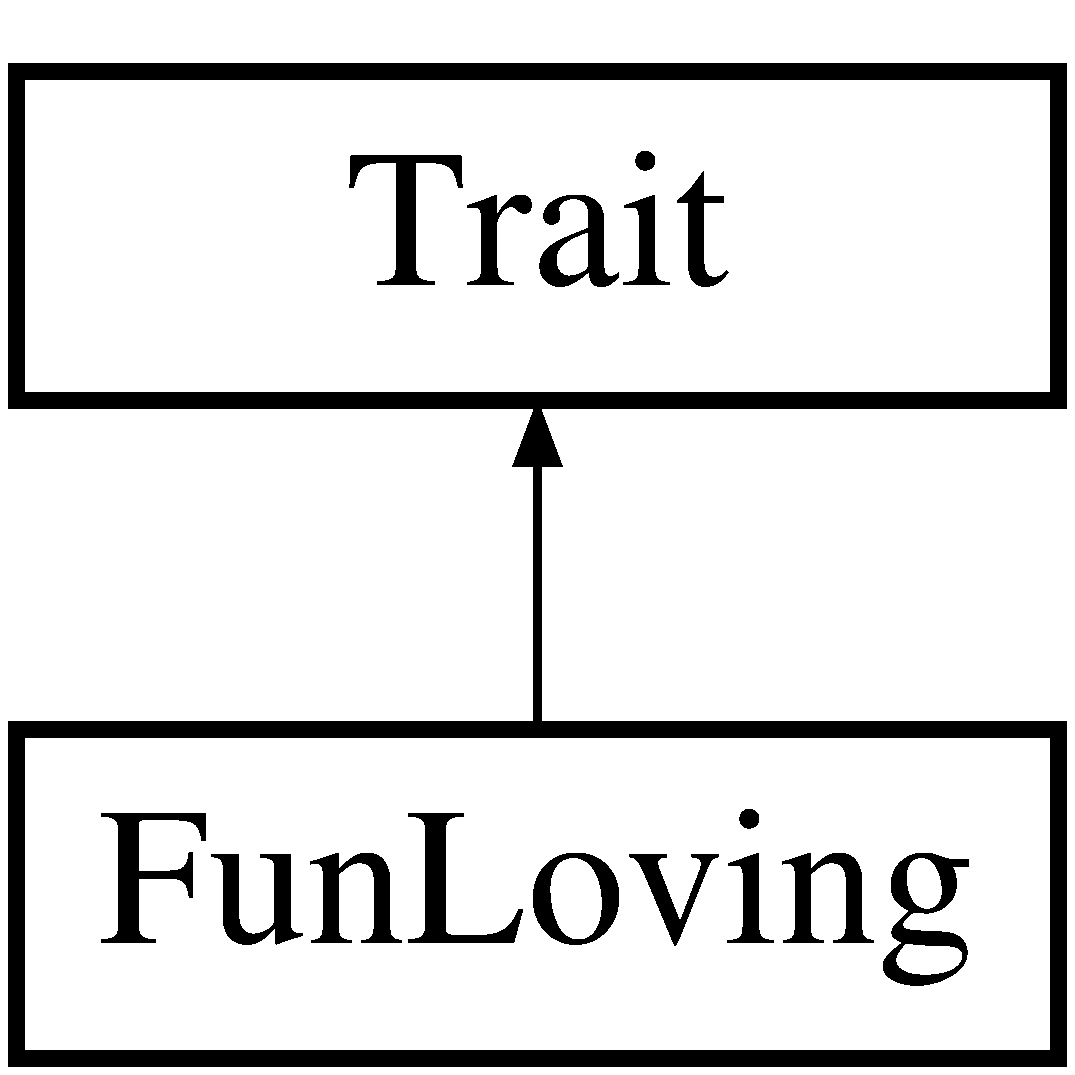
\includegraphics[height=2.000000cm]{class_fun_loving}
\end{center}
\end{figure}
\subsection*{Public Member Functions}
\begin{DoxyCompactItemize}
\item 
\hyperlink{class_fun_loving_a8e2a0b7a1fc6658f6f1c5a16b35dc5e6}{Fun\-Loving} (void)
\begin{DoxyCompactList}\small\item\em Default constructor. \end{DoxyCompactList}\item 
\hyperlink{class_fun_loving_a1aba0ea1aab424eb82e2bece61b9d432}{$\sim$\-Fun\-Loving} (void)
\begin{DoxyCompactList}\small\item\em Destructor. \end{DoxyCompactList}\end{DoxyCompactItemize}


\subsection{Detailed Description}
Fun loving. 

\begin{DoxyAuthor}{Author}
Hamish Carrier 
\end{DoxyAuthor}
\begin{DoxyDate}{Date}
10/11/2013 
\end{DoxyDate}


\subsection{Constructor \& Destructor Documentation}
\hypertarget{class_fun_loving_a8e2a0b7a1fc6658f6f1c5a16b35dc5e6}{\index{Fun\-Loving@{Fun\-Loving}!Fun\-Loving@{Fun\-Loving}}
\index{Fun\-Loving@{Fun\-Loving}!FunLoving@{Fun\-Loving}}
\subsubsection[{Fun\-Loving}]{\setlength{\rightskip}{0pt plus 5cm}Fun\-Loving\-::\-Fun\-Loving (
\begin{DoxyParamCaption}
\item[{void}]{}
\end{DoxyParamCaption}
)}}\label{class_fun_loving_a8e2a0b7a1fc6658f6f1c5a16b35dc5e6}


Default constructor. 

\begin{DoxyAuthor}{Author}
Hamish Carrier 
\end{DoxyAuthor}
\begin{DoxyDate}{Date}
10/11/2013 
\end{DoxyDate}
\hypertarget{class_fun_loving_a1aba0ea1aab424eb82e2bece61b9d432}{\index{Fun\-Loving@{Fun\-Loving}!$\sim$\-Fun\-Loving@{$\sim$\-Fun\-Loving}}
\index{$\sim$\-Fun\-Loving@{$\sim$\-Fun\-Loving}!FunLoving@{Fun\-Loving}}
\subsubsection[{$\sim$\-Fun\-Loving}]{\setlength{\rightskip}{0pt plus 5cm}Fun\-Loving\-::$\sim$\-Fun\-Loving (
\begin{DoxyParamCaption}
\item[{void}]{}
\end{DoxyParamCaption}
)}}\label{class_fun_loving_a1aba0ea1aab424eb82e2bece61b9d432}


Destructor. 

\begin{DoxyAuthor}{Author}
Hamish Carrier 
\end{DoxyAuthor}
\begin{DoxyDate}{Date}
10/11/2013 
\end{DoxyDate}


The documentation for this class was generated from the following files\-:\begin{DoxyCompactItemize}
\item 
A\-:/\-I\-T/\-Git\-Hub/\-I\-C\-T312/source/ogregraphics/\hyperlink{_fun_loving_8h}{Fun\-Loving.\-h}\item 
A\-:/\-I\-T/\-Git\-Hub/\-I\-C\-T312/source/ogregraphics/Fun\-Loving.\-cpp\end{DoxyCompactItemize}

\hypertarget{class_core_1_1_game}{\section{Core\-:\-:Game Class Reference}
\label{class_core_1_1_game}\index{Core\-::\-Game@{Core\-::\-Game}}
}
\subsection*{Static Public Member Functions}
\begin{DoxyCompactItemize}
\item 
\hypertarget{class_core_1_1_game_a776a825379f2dc026358b5f278500c90}{static int {\bfseries initialise} ()}\label{class_core_1_1_game_a776a825379f2dc026358b5f278500c90}

\item 
\hypertarget{class_core_1_1_game_aede5f46c8c7bbbaf8459eeec397a11e7}{static void {\bfseries game\-Loop} ()}\label{class_core_1_1_game_aede5f46c8c7bbbaf8459eeec397a11e7}

\item 
\hypertarget{class_core_1_1_game_af11feb29c5399b360bd5740d0fd1b5d4}{static bool {\bfseries get\-Running} ()}\label{class_core_1_1_game_af11feb29c5399b360bd5740d0fd1b5d4}

\item 
\hypertarget{class_core_1_1_game_a80dd6cde2747fad68d18719f3dd1cbe1}{static void {\bfseries set\-Running} (bool running)}\label{class_core_1_1_game_a80dd6cde2747fad68d18719f3dd1cbe1}

\item 
\hypertarget{class_core_1_1_game_ad7fa5bdf71ea8e2ac3057a54e50b087e}{static \hyperlink{class_graphics_1_1_ogre_graphics}{Graphics\-::\-Ogre\-Graphics} $\ast$ {\bfseries get\-Graphics} ()}\label{class_core_1_1_game_ad7fa5bdf71ea8e2ac3057a54e50b087e}

\item 
\hypertarget{class_core_1_1_game_a103f4fe333cd90ba01dd25073fd3143e}{static \hyperlink{class_scenes_1_1_scene_manager}{Scenes\-::\-Scene\-Manager} $\ast$ {\bfseries get\-Scene\-Manager} ()}\label{class_core_1_1_game_a103f4fe333cd90ba01dd25073fd3143e}

\item 
\hypertarget{class_core_1_1_game_a9f0e2e31c03a7e28012f16d9e57acbd1}{static O\-I\-S\-::\-Input\-Manager $\ast$ {\bfseries get\-Input\-Manager} ()}\label{class_core_1_1_game_a9f0e2e31c03a7e28012f16d9e57acbd1}

\item 
\hypertarget{class_core_1_1_game_accf9a2d029a5e29750063f17afd34702}{static O\-I\-S\-::\-Keyboard $\ast$ {\bfseries get\-Keyboard} ()}\label{class_core_1_1_game_accf9a2d029a5e29750063f17afd34702}

\item 
\hypertarget{class_core_1_1_game_a73128fb8a1e880ead8b7037604094c3c}{static O\-I\-S\-::\-Mouse $\ast$ {\bfseries get\-Mouse} ()}\label{class_core_1_1_game_a73128fb8a1e880ead8b7037604094c3c}

\item 
static void \hyperlink{class_core_1_1_game_adcc42940f3a8ec29a5d8a7a8f0cfaba1}{Test\-Select} ()
\begin{DoxyCompactList}\small\item\em This is a raycasting function for triggering a response in A\-I. \end{DoxyCompactList}\item 
static void \hyperlink{class_core_1_1_game_a08c63cc8fca9799addc42df08548f623}{Set\-Affordances} ()
\begin{DoxyCompactList}\small\item\em Sets affordances for objects in the world. \end{DoxyCompactList}\end{DoxyCompactItemize}


\subsection{Member Function Documentation}
\hypertarget{class_core_1_1_game_a08c63cc8fca9799addc42df08548f623}{\index{Core\-::\-Game@{Core\-::\-Game}!Set\-Affordances@{Set\-Affordances}}
\index{Set\-Affordances@{Set\-Affordances}!Core::Game@{Core\-::\-Game}}
\subsubsection[{Set\-Affordances}]{\setlength{\rightskip}{0pt plus 5cm}static void Core\-::\-Game\-::\-Set\-Affordances (
\begin{DoxyParamCaption}
{}
\end{DoxyParamCaption}
)\hspace{0.3cm}{\ttfamily [static]}}}\label{class_core_1_1_game_a08c63cc8fca9799addc42df08548f623}


Sets affordances for objects in the world. 

\begin{DoxyAuthor}{Author}
Arran Ford 
\end{DoxyAuthor}
\begin{DoxyDate}{Date}
09/11/2013 
\end{DoxyDate}
\hypertarget{class_core_1_1_game_adcc42940f3a8ec29a5d8a7a8f0cfaba1}{\index{Core\-::\-Game@{Core\-::\-Game}!Test\-Select@{Test\-Select}}
\index{Test\-Select@{Test\-Select}!Core::Game@{Core\-::\-Game}}
\subsubsection[{Test\-Select}]{\setlength{\rightskip}{0pt plus 5cm}static void Core\-::\-Game\-::\-Test\-Select (
\begin{DoxyParamCaption}
{}
\end{DoxyParamCaption}
)\hspace{0.3cm}{\ttfamily [static]}}}\label{class_core_1_1_game_adcc42940f3a8ec29a5d8a7a8f0cfaba1}


This is a raycasting function for triggering a response in A\-I. 

\begin{DoxyAuthor}{Author}
Arran Ford 
\end{DoxyAuthor}
\begin{DoxyDate}{Date}
09/11/2013 
\end{DoxyDate}


The documentation for this class was generated from the following files\-:\begin{DoxyCompactItemize}
\item 
A\-:/\-I\-T/\-Git\-Hub/\-I\-C\-T312/source/ogregraphics/Game.\-h\item 
A\-:/\-I\-T/\-Git\-Hub/\-I\-C\-T312/source/ogregraphics/Game.\-cpp\end{DoxyCompactItemize}

\hypertarget{class_objects_1_1_generic_object}{\section{Objects\-:\-:Generic\-Object Class Reference}
\label{class_objects_1_1_generic_object}\index{Objects\-::\-Generic\-Object@{Objects\-::\-Generic\-Object}}
}


Generic object.  




{\ttfamily \#include $<$Generic\-Object.\-h$>$}

Inheritance diagram for Objects\-:\-:Generic\-Object\-:\begin{figure}[H]
\begin{center}
\leavevmode
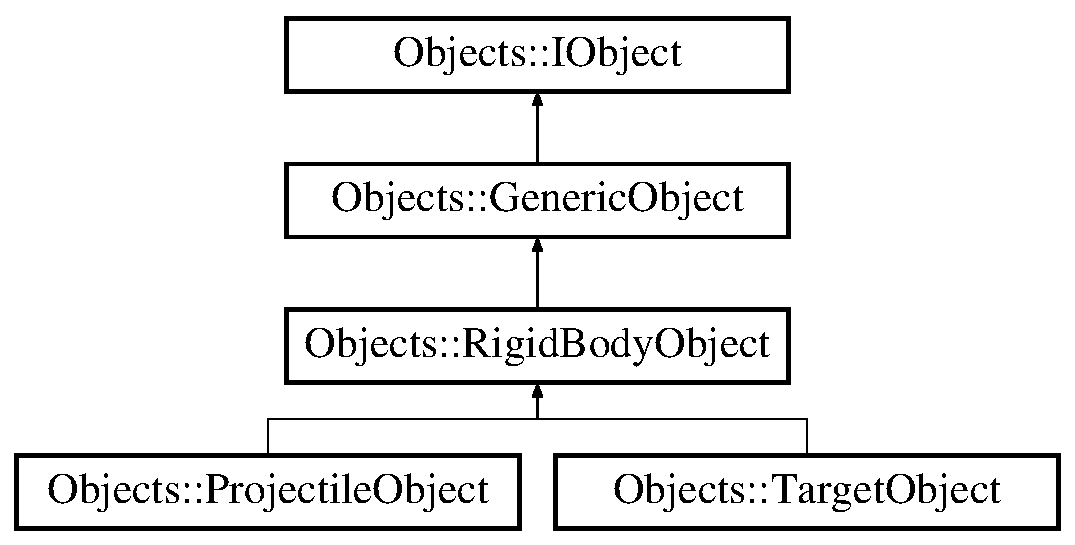
\includegraphics[height=4.000000cm]{class_objects_1_1_generic_object}
\end{center}
\end{figure}
\subsection*{Public Member Functions}
\begin{DoxyCompactItemize}
\item 
\hypertarget{class_objects_1_1_generic_object_abeb3e050cbd3e1458e0d73ccb5feb13b}{\hyperlink{class_objects_1_1_generic_object_abeb3e050cbd3e1458e0d73ccb5feb13b}{Generic\-Object} ()}\label{class_objects_1_1_generic_object_abeb3e050cbd3e1458e0d73ccb5feb13b}

\begin{DoxyCompactList}\small\item\em Default constructor. \end{DoxyCompactList}\item 
\hyperlink{class_objects_1_1_generic_object_af2dbae8570212439ea7c8b7dd8be5f4c}{Generic\-Object} (Ogre\-::\-Vector3 pos, Ogre\-::\-Vector3 rot, std\-::string mesh\-File)
\begin{DoxyCompactList}\small\item\em Constructor. \end{DoxyCompactList}\item 
\hyperlink{class_objects_1_1_generic_object_a3b2acd7559918edcbc74bd7d20da9763}{Generic\-Object} (Ogre\-::\-Vector3 pos, Ogre\-::\-Quaternion rot, Ogre\-::\-Vector3 scale, std\-::string mesh\-File)
\begin{DoxyCompactList}\small\item\em Constructor. \end{DoxyCompactList}\item 
\hypertarget{class_objects_1_1_generic_object_afb238b6fb112b4fb32e1180fab1fc68d}{\hyperlink{class_objects_1_1_generic_object_afb238b6fb112b4fb32e1180fab1fc68d}{$\sim$\-Generic\-Object} (void)}\label{class_objects_1_1_generic_object_afb238b6fb112b4fb32e1180fab1fc68d}

\begin{DoxyCompactList}\small\item\em Destructor. \end{DoxyCompactList}\item 
\hypertarget{class_objects_1_1_generic_object_a348bb3c00151b9824863a7b591b4b529}{virtual void \hyperlink{class_objects_1_1_generic_object_a348bb3c00151b9824863a7b591b4b529}{initialise} ()}\label{class_objects_1_1_generic_object_a348bb3c00151b9824863a7b591b4b529}

\begin{DoxyCompactList}\small\item\em bool Generic; \end{DoxyCompactList}\item 
virtual void \hyperlink{class_objects_1_1_generic_object_a57c85bdf2ceb1ffa1b85ec3aa51a631d}{update} (float delta\-Time)
\begin{DoxyCompactList}\small\item\em Updates the given delta\-Time. \end{DoxyCompactList}\end{DoxyCompactItemize}
\subsection*{Additional Inherited Members}


\subsection{Detailed Description}
Generic object. 

\subsection{Constructor \& Destructor Documentation}
\hypertarget{class_objects_1_1_generic_object_af2dbae8570212439ea7c8b7dd8be5f4c}{\index{Objects\-::\-Generic\-Object@{Objects\-::\-Generic\-Object}!Generic\-Object@{Generic\-Object}}
\index{Generic\-Object@{Generic\-Object}!Objects::GenericObject@{Objects\-::\-Generic\-Object}}
\subsubsection[{Generic\-Object}]{\setlength{\rightskip}{0pt plus 5cm}Objects\-::\-Generic\-Object\-::\-Generic\-Object (
\begin{DoxyParamCaption}
\item[{Ogre\-::\-Vector3}]{pos, }
\item[{Ogre\-::\-Vector3}]{rot, }
\item[{std\-::string}]{mesh\-File}
\end{DoxyParamCaption}
)}}\label{class_objects_1_1_generic_object_af2dbae8570212439ea7c8b7dd8be5f4c}


Constructor. 


\begin{DoxyParams}{Parameters}
{\em pos} & The position. \\
\hline
{\em rot} & The rot. \\
\hline
{\em mesh\-File} & The mesh file. \\
\hline
\end{DoxyParams}
\hypertarget{class_objects_1_1_generic_object_a3b2acd7559918edcbc74bd7d20da9763}{\index{Objects\-::\-Generic\-Object@{Objects\-::\-Generic\-Object}!Generic\-Object@{Generic\-Object}}
\index{Generic\-Object@{Generic\-Object}!Objects::GenericObject@{Objects\-::\-Generic\-Object}}
\subsubsection[{Generic\-Object}]{\setlength{\rightskip}{0pt plus 5cm}Objects\-::\-Generic\-Object\-::\-Generic\-Object (
\begin{DoxyParamCaption}
\item[{Ogre\-::\-Vector3}]{pos, }
\item[{Ogre\-::\-Quaternion}]{rot, }
\item[{Ogre\-::\-Vector3}]{scale, }
\item[{std\-::string}]{mesh\-File}
\end{DoxyParamCaption}
)}}\label{class_objects_1_1_generic_object_a3b2acd7559918edcbc74bd7d20da9763}


Constructor. 


\begin{DoxyParams}{Parameters}
{\em pos} & The position. \\
\hline
{\em rot} & The rot. \\
\hline
{\em scale} & The scale. \\
\hline
{\em mesh\-File} & The mesh file. \\
\hline
\end{DoxyParams}


\subsection{Member Function Documentation}
\hypertarget{class_objects_1_1_generic_object_a57c85bdf2ceb1ffa1b85ec3aa51a631d}{\index{Objects\-::\-Generic\-Object@{Objects\-::\-Generic\-Object}!update@{update}}
\index{update@{update}!Objects::GenericObject@{Objects\-::\-Generic\-Object}}
\subsubsection[{update}]{\setlength{\rightskip}{0pt plus 5cm}void Objects\-::\-Generic\-Object\-::update (
\begin{DoxyParamCaption}
\item[{float}]{delta\-Time}
\end{DoxyParamCaption}
)\hspace{0.3cm}{\ttfamily [virtual]}}}\label{class_objects_1_1_generic_object_a57c85bdf2ceb1ffa1b85ec3aa51a631d}


Updates the given delta\-Time. 


\begin{DoxyParams}{Parameters}
{\em delta\-Time} & Time of the delta. \\
\hline
\end{DoxyParams}


Reimplemented from \hyperlink{class_objects_1_1_i_object_a616e6befc5fbdca47155b1b56d0e0fc0}{Objects\-::\-I\-Object}.



Reimplemented in \hyperlink{class_objects_1_1_rigid_body_object_a478edcbc5820722a9641fdcd07b402bb}{Objects\-::\-Rigid\-Body\-Object}, \hyperlink{class_objects_1_1_target_object_a46b8163c5921925aa6d95fc0e99ce011}{Objects\-::\-Target\-Object}, and \hyperlink{class_objects_1_1_projectile_object_ae8cb3b7f7a9f5b921b043a58e9e355dc}{Objects\-::\-Projectile\-Object}.



The documentation for this class was generated from the following files\-:\begin{DoxyCompactItemize}
\item 
A\-:/\-I\-T/\-Git\-Hub/\-I\-C\-T312/source/ogregraphics/\hyperlink{_generic_object_8h}{Generic\-Object.\-h}\item 
A\-:/\-I\-T/\-Git\-Hub/\-I\-C\-T312/source/ogregraphics/Generic\-Object.\-cpp\end{DoxyCompactItemize}

\hypertarget{class_goal}{\section{Goal Class Reference}
\label{class_goal}\index{Goal@{Goal}}
}


\hyperlink{class_goal}{Goal}.  




{\ttfamily \#include $<$Goal.\-h$>$}

Inheritance diagram for Goal\-:\begin{figure}[H]
\begin{center}
\leavevmode
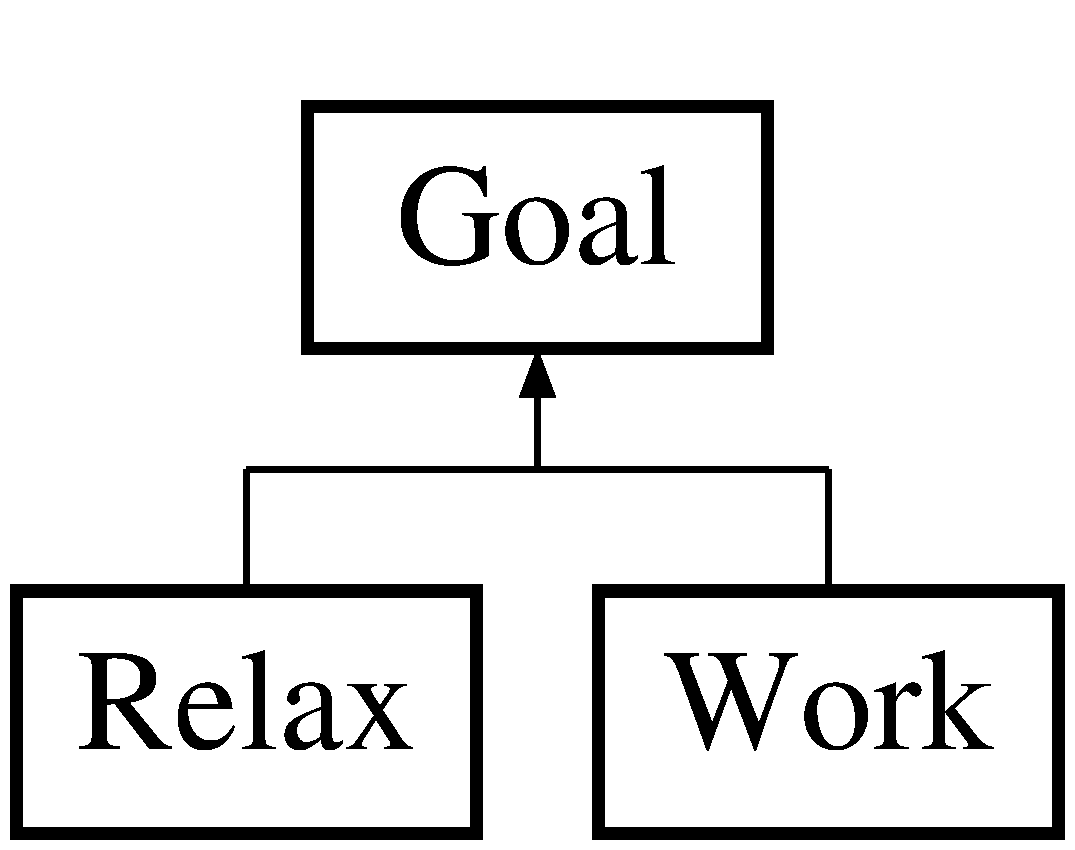
\includegraphics[height=2.000000cm]{class_goal}
\end{center}
\end{figure}


\subsection{Detailed Description}
\hyperlink{class_goal}{Goal}. 

\begin{DoxyAuthor}{Author}
Hamish Carrier 
\end{DoxyAuthor}
\begin{DoxyDate}{Date}
10/11/2013 
\end{DoxyDate}


The documentation for this class was generated from the following file\-:\begin{DoxyCompactItemize}
\item 
A\-:/\-I\-T/\-Git\-Hub/\-I\-C\-T312/source/ogregraphics/\hyperlink{_goal_8h}{Goal.\-h}\end{DoxyCompactItemize}

\hypertarget{class_good}{\section{Good Class Reference}
\label{class_good}\index{Good@{Good}}
}


\hyperlink{class_good}{Good}.  




{\ttfamily \#include $<$Good.\-h$>$}

Inheritance diagram for Good\-:\begin{figure}[H]
\begin{center}
\leavevmode
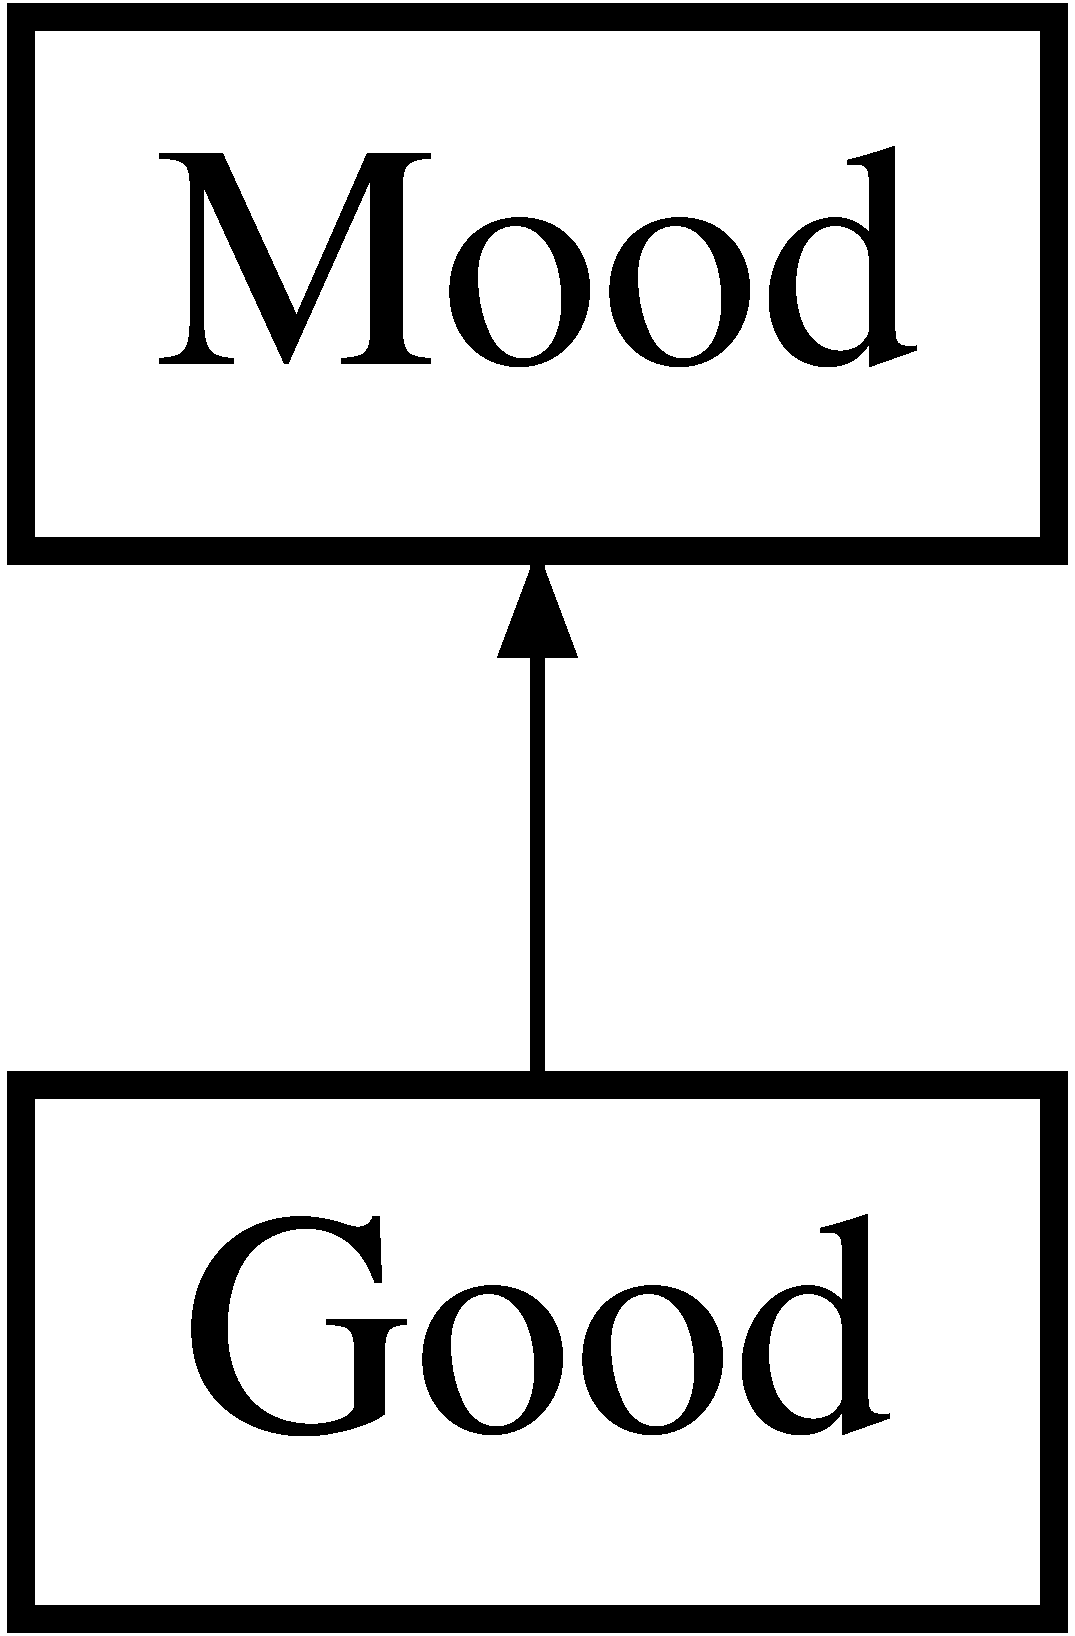
\includegraphics[height=2.000000cm]{class_good}
\end{center}
\end{figure}
\subsection*{Public Member Functions}
\begin{DoxyCompactItemize}
\item 
\hyperlink{class_good_a09ffd1e3d5efc7bb9aea3e1b14b029ca}{Good} (void)
\begin{DoxyCompactList}\small\item\em Default constructor. \end{DoxyCompactList}\item 
\hyperlink{class_good_a3c3cb457fe82ced67e264a878a5d5ce3}{$\sim$\-Good} (void)
\begin{DoxyCompactList}\small\item\em Destructor. \end{DoxyCompactList}\end{DoxyCompactItemize}


\subsection{Detailed Description}
\hyperlink{class_good}{Good}. 

\begin{DoxyAuthor}{Author}
Hamish Carrier 
\end{DoxyAuthor}
\begin{DoxyDate}{Date}
10/11/2013 
\end{DoxyDate}


\subsection{Constructor \& Destructor Documentation}
\hypertarget{class_good_a09ffd1e3d5efc7bb9aea3e1b14b029ca}{\index{Good@{Good}!Good@{Good}}
\index{Good@{Good}!Good@{Good}}
\subsubsection[{Good}]{\setlength{\rightskip}{0pt plus 5cm}Good\-::\-Good (
\begin{DoxyParamCaption}
\item[{void}]{}
\end{DoxyParamCaption}
)}}\label{class_good_a09ffd1e3d5efc7bb9aea3e1b14b029ca}


Default constructor. 

\begin{DoxyAuthor}{Author}
Hamish Carrier 
\end{DoxyAuthor}
\begin{DoxyDate}{Date}
10/11/2013 
\end{DoxyDate}
\hypertarget{class_good_a3c3cb457fe82ced67e264a878a5d5ce3}{\index{Good@{Good}!$\sim$\-Good@{$\sim$\-Good}}
\index{$\sim$\-Good@{$\sim$\-Good}!Good@{Good}}
\subsubsection[{$\sim$\-Good}]{\setlength{\rightskip}{0pt plus 5cm}Good\-::$\sim$\-Good (
\begin{DoxyParamCaption}
\item[{void}]{}
\end{DoxyParamCaption}
)}}\label{class_good_a3c3cb457fe82ced67e264a878a5d5ce3}


Destructor. 

\begin{DoxyAuthor}{Author}
Hamish Carrier 
\end{DoxyAuthor}
\begin{DoxyDate}{Date}
10/11/2013 
\end{DoxyDate}


The documentation for this class was generated from the following files\-:\begin{DoxyCompactItemize}
\item 
A\-:/\-I\-T/\-Git\-Hub/\-I\-C\-T312/source/ogregraphics/\hyperlink{_good_8h}{Good.\-h}\item 
A\-:/\-I\-T/\-Git\-Hub/\-I\-C\-T312/source/ogregraphics/Good.\-cpp\end{DoxyCompactItemize}

\hypertarget{classmicropather_1_1_graph}{\section{micropather\-:\-:Graph Class Reference}
\label{classmicropather_1_1_graph}\index{micropather\-::\-Graph@{micropather\-::\-Graph}}
}


{\ttfamily \#include $<$micropather.\-h$>$}

Inheritance diagram for micropather\-:\-:Graph\-:\begin{figure}[H]
\begin{center}
\leavevmode
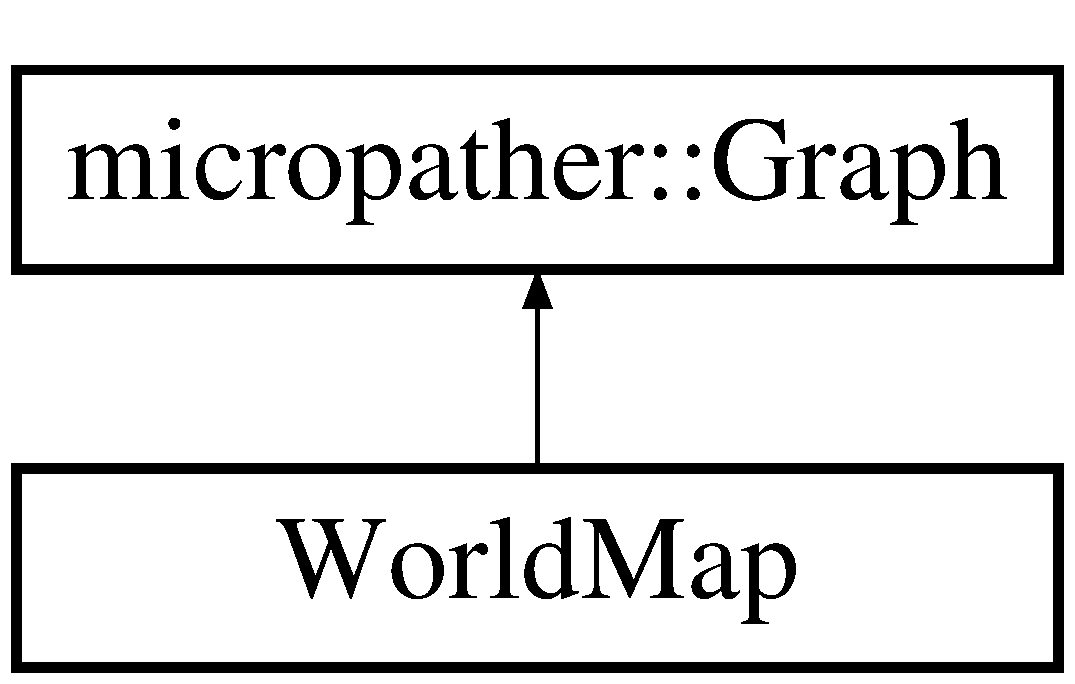
\includegraphics[height=2.000000cm]{classmicropather_1_1_graph}
\end{center}
\end{figure}
\subsection*{Public Member Functions}
\begin{DoxyCompactItemize}
\item 
virtual float \hyperlink{classmicropather_1_1_graph_a7a284a95607553e15439ecc7a1440abc}{Least\-Cost\-Estimate} (void $\ast$state\-Start, void $\ast$state\-End)=0
\item 
virtual void \hyperlink{classmicropather_1_1_graph_acc601fe0c8f0774e37208c9e15eba00a}{Adjacent\-Cost} (void $\ast$state, std\-::vector$<$ \hyperlink{structmicropather_1_1_state_cost}{micropather\-::\-State\-Cost} $>$ $\ast$adjacent)=0
\item 
virtual void \hyperlink{classmicropather_1_1_graph_a9ca57ce2dceccece9654545b7dfad6ff}{Print\-State\-Info} (void $\ast$state)=0
\end{DoxyCompactItemize}


\subsection{Detailed Description}
A pure abstract class used to define a set of callbacks. The client application inherits from this class, and the methods will be called when \hyperlink{classmicropather_1_1_micro_pather_af81b5dad8f89610026b8f0762d981730}{Micro\-Pather\-::\-Solve()} is invoked.

The notion of a \char`\"{}state\char`\"{} is very important. It must have the following properties\-:
\begin{DoxyItemize}
\item Unique
\item Unchanging (unless \hyperlink{classmicropather_1_1_micro_pather_aa830a9fa99403c14c6791f513a8e2342}{Micro\-Pather\-::\-Reset()} is called)
\end{DoxyItemize}

If the client application represents states as objects, then the state is usually just the object cast to a void$\ast$. If the client application sees states as numerical values, (x,y) for example, then state is an encoding of these values. \hyperlink{classmicropather_1_1_micro_pather}{Micro\-Pather} never interprets or modifies the value of state. 

\subsection{Member Function Documentation}
\hypertarget{classmicropather_1_1_graph_acc601fe0c8f0774e37208c9e15eba00a}{\index{micropather\-::\-Graph@{micropather\-::\-Graph}!Adjacent\-Cost@{Adjacent\-Cost}}
\index{Adjacent\-Cost@{Adjacent\-Cost}!micropather::Graph@{micropather\-::\-Graph}}
\subsubsection[{Adjacent\-Cost}]{\setlength{\rightskip}{0pt plus 5cm}virtual void micropather\-::\-Graph\-::\-Adjacent\-Cost (
\begin{DoxyParamCaption}
\item[{void $\ast$}]{state, }
\item[{std\-::vector$<$ {\bf micropather\-::\-State\-Cost} $>$ $\ast$}]{adjacent}
\end{DoxyParamCaption}
)\hspace{0.3cm}{\ttfamily [pure virtual]}}}\label{classmicropather_1_1_graph_acc601fe0c8f0774e37208c9e15eba00a}
Return the exact cost from the given state to all its neighboring states. This may be called multiple times, or cached by the solver. It {\itshape must} return the same exact values for every call to \hyperlink{classmicropather_1_1_micro_pather_af81b5dad8f89610026b8f0762d981730}{Micro\-Pather\-::\-Solve()}. It should generally be a simple, fast function with no callbacks into the pather. \hypertarget{classmicropather_1_1_graph_a7a284a95607553e15439ecc7a1440abc}{\index{micropather\-::\-Graph@{micropather\-::\-Graph}!Least\-Cost\-Estimate@{Least\-Cost\-Estimate}}
\index{Least\-Cost\-Estimate@{Least\-Cost\-Estimate}!micropather::Graph@{micropather\-::\-Graph}}
\subsubsection[{Least\-Cost\-Estimate}]{\setlength{\rightskip}{0pt plus 5cm}virtual float micropather\-::\-Graph\-::\-Least\-Cost\-Estimate (
\begin{DoxyParamCaption}
\item[{void $\ast$}]{state\-Start, }
\item[{void $\ast$}]{state\-End}
\end{DoxyParamCaption}
)\hspace{0.3cm}{\ttfamily [pure virtual]}}}\label{classmicropather_1_1_graph_a7a284a95607553e15439ecc7a1440abc}
Return the least possible cost between 2 states. For example, if your pathfinding is based on distance, this is simply the straight distance between 2 points on the map. If you pathfinding is based on minimum time, it is the minimal travel time between 2 points given the best possible terrain. 

Implemented in \hyperlink{class_world_map_a1303b34f21eed11133f8e9895f30121b}{World\-Map}.

\hypertarget{classmicropather_1_1_graph_a9ca57ce2dceccece9654545b7dfad6ff}{\index{micropather\-::\-Graph@{micropather\-::\-Graph}!Print\-State\-Info@{Print\-State\-Info}}
\index{Print\-State\-Info@{Print\-State\-Info}!micropather::Graph@{micropather\-::\-Graph}}
\subsubsection[{Print\-State\-Info}]{\setlength{\rightskip}{0pt plus 5cm}virtual void micropather\-::\-Graph\-::\-Print\-State\-Info (
\begin{DoxyParamCaption}
\item[{void $\ast$}]{state}
\end{DoxyParamCaption}
)\hspace{0.3cm}{\ttfamily [pure virtual]}}}\label{classmicropather_1_1_graph_a9ca57ce2dceccece9654545b7dfad6ff}
This function is only used in D\-E\-B\-U\-G mode -\/ it dumps output to stdout. Since void$\ast$ aren't really human readable, normally you print out some concise info (like \char`\"{}(1,2)\char`\"{}) without an ending newline. 

Implemented in \hyperlink{class_world_map_a545c1c031a72cc21ec4c7e9d6103fad7}{World\-Map}.



The documentation for this class was generated from the following file\-:\begin{DoxyCompactItemize}
\item 
A\-:/\-I\-T/\-Git\-Hub/\-I\-C\-T312/source/ogregraphics/micropather.\-h\end{DoxyCompactItemize}

\hypertarget{class_happy}{\section{Happy Class Reference}
\label{class_happy}\index{Happy@{Happy}}
}


\hyperlink{class_happy}{Happy}.  




{\ttfamily \#include $<$Happy.\-h$>$}

Inheritance diagram for Happy\-:\begin{figure}[H]
\begin{center}
\leavevmode
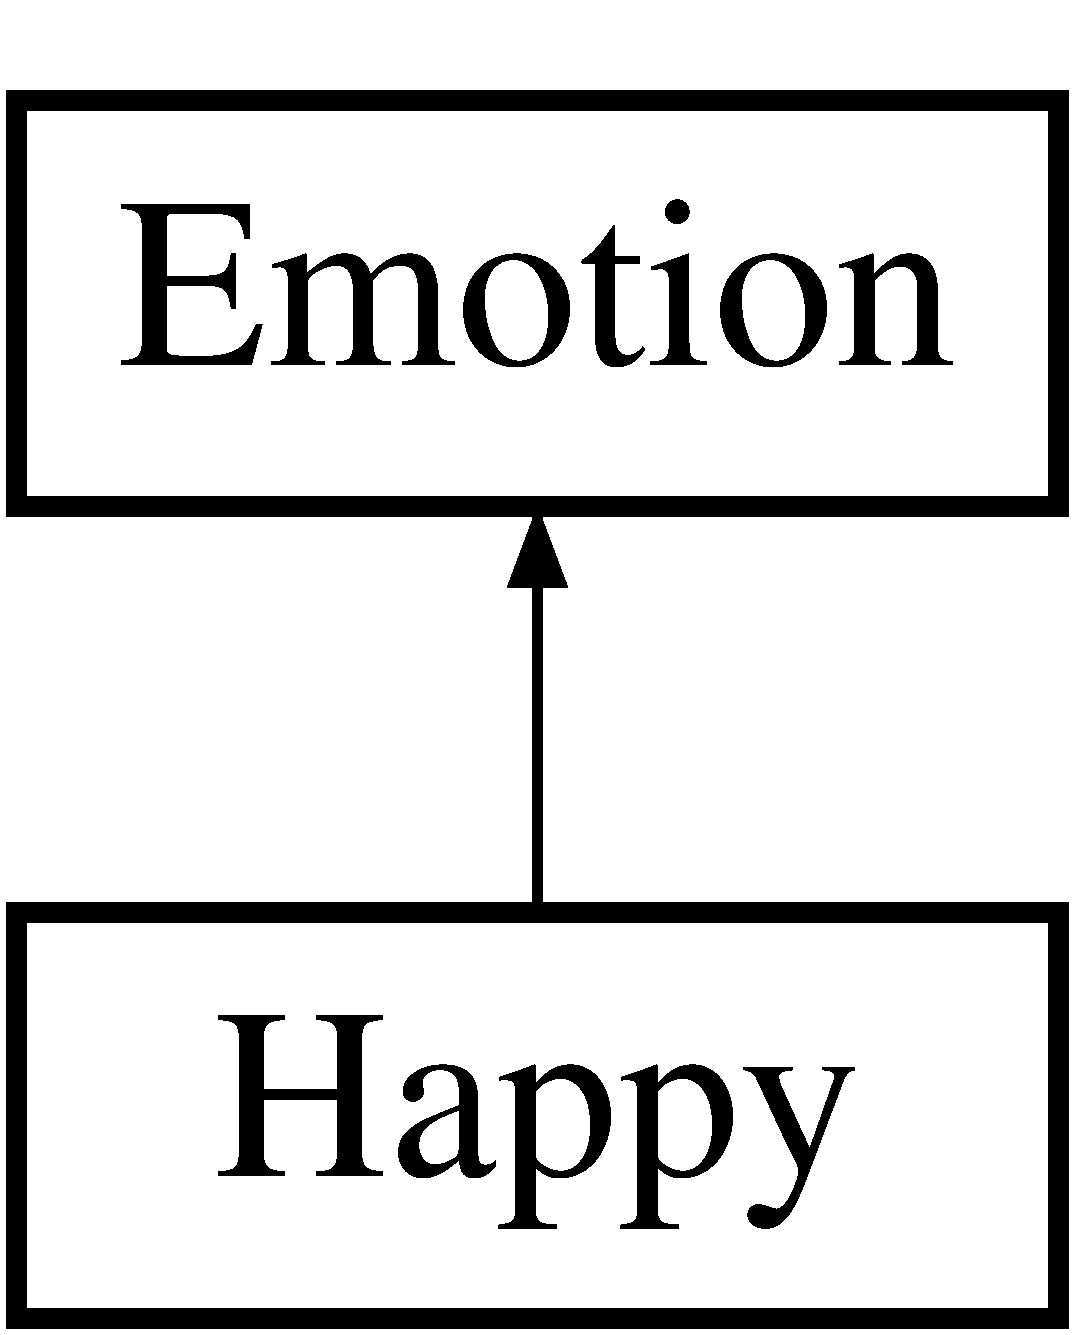
\includegraphics[height=2.000000cm]{class_happy}
\end{center}
\end{figure}
\subsection*{Public Member Functions}
\begin{DoxyCompactItemize}
\item 
\hyperlink{class_happy_a36541141c0239f5e3ce0124f4b5f36c2}{Happy} (void)
\begin{DoxyCompactList}\small\item\em Default constructor. \end{DoxyCompactList}\item 
\hyperlink{class_happy_a40ee1fcd94422aca50e782ab668be834}{$\sim$\-Happy} (void)
\begin{DoxyCompactList}\small\item\em Destructor. \end{DoxyCompactList}\end{DoxyCompactItemize}


\subsection{Detailed Description}
\hyperlink{class_happy}{Happy}. 

\begin{DoxyAuthor}{Author}
Hamish Carrier 
\end{DoxyAuthor}
\begin{DoxyDate}{Date}
10/11/2013 
\end{DoxyDate}


\subsection{Constructor \& Destructor Documentation}
\hypertarget{class_happy_a36541141c0239f5e3ce0124f4b5f36c2}{\index{Happy@{Happy}!Happy@{Happy}}
\index{Happy@{Happy}!Happy@{Happy}}
\subsubsection[{Happy}]{\setlength{\rightskip}{0pt plus 5cm}Happy\-::\-Happy (
\begin{DoxyParamCaption}
\item[{void}]{}
\end{DoxyParamCaption}
)}}\label{class_happy_a36541141c0239f5e3ce0124f4b5f36c2}


Default constructor. 

\begin{DoxyAuthor}{Author}
Hamish Carrier 
\end{DoxyAuthor}
\begin{DoxyDate}{Date}
10/11/2013 
\end{DoxyDate}
\hypertarget{class_happy_a40ee1fcd94422aca50e782ab668be834}{\index{Happy@{Happy}!$\sim$\-Happy@{$\sim$\-Happy}}
\index{$\sim$\-Happy@{$\sim$\-Happy}!Happy@{Happy}}
\subsubsection[{$\sim$\-Happy}]{\setlength{\rightskip}{0pt plus 5cm}Happy\-::$\sim$\-Happy (
\begin{DoxyParamCaption}
\item[{void}]{}
\end{DoxyParamCaption}
)}}\label{class_happy_a40ee1fcd94422aca50e782ab668be834}


Destructor. 

\begin{DoxyAuthor}{Author}
Hamish Carrier 
\end{DoxyAuthor}
\begin{DoxyDate}{Date}
10/11/2013 
\end{DoxyDate}


The documentation for this class was generated from the following files\-:\begin{DoxyCompactItemize}
\item 
A\-:/\-I\-T/\-Git\-Hub/\-I\-C\-T312/source/ogregraphics/\hyperlink{_happy_8h}{Happy.\-h}\item 
A\-:/\-I\-T/\-Git\-Hub/\-I\-C\-T312/source/ogregraphics/Happy.\-cpp\end{DoxyCompactItemize}

\hypertarget{class_ico_sphere}{\section{Ico\-Sphere Class Reference}
\label{class_ico_sphere}\index{Ico\-Sphere@{Ico\-Sphere}}
}
\subsection*{Classes}
\begin{DoxyCompactItemize}
\item 
struct \hyperlink{struct_ico_sphere_1_1_line_indices}{Line\-Indices}
\item 
struct \hyperlink{struct_ico_sphere_1_1_triangle_indices}{Triangle\-Indices}
\end{DoxyCompactItemize}
\subsection*{Public Member Functions}
\begin{DoxyCompactItemize}
\item 
\hypertarget{class_ico_sphere_a5b1db233e62838146ead7c3d838b24c4}{void {\bfseries create} (int recursion\-Level)}\label{class_ico_sphere_a5b1db233e62838146ead7c3d838b24c4}

\item 
\hypertarget{class_ico_sphere_ac39677216ad01911484b808e12c61b54}{void {\bfseries add\-To\-Line\-Indices} (int base\-Index, std\-::list$<$ int $>$ $\ast$target)}\label{class_ico_sphere_ac39677216ad01911484b808e12c61b54}

\item 
\hypertarget{class_ico_sphere_af1b260dd184f18e50dd00d6f8bd1a6e2}{int {\bfseries add\-To\-Vertices} (std\-::list$<$ Vertex\-Pair $>$ $\ast$target, const Ogre\-::\-Vector3 \&position, const Ogre\-::\-Colour\-Value \&colour, float scale)}\label{class_ico_sphere_af1b260dd184f18e50dd00d6f8bd1a6e2}

\item 
\hypertarget{class_ico_sphere_af4bbaf3ab2a0d645d565c52c540a2a39}{void {\bfseries add\-To\-Triangle\-Indices} (int base\-Index, std\-::list$<$ int $>$ $\ast$target)}\label{class_ico_sphere_af4bbaf3ab2a0d645d565c52c540a2a39}

\end{DoxyCompactItemize}


The documentation for this class was generated from the following files\-:\begin{DoxyCompactItemize}
\item 
A\-:/\-I\-T/\-Git\-Hub/\-I\-C\-T312/source/ogregraphics/Debug\-Drawer.\-h\item 
A\-:/\-I\-T/\-Git\-Hub/\-I\-C\-T312/source/ogregraphics/Debug\-Drawer.\-cpp\end{DoxyCompactItemize}

\hypertarget{class_objects_1_1_i_object}{\section{Objects\-:\-:I\-Object Class Reference}
\label{class_objects_1_1_i_object}\index{Objects\-::\-I\-Object@{Objects\-::\-I\-Object}}
}


Object.  




{\ttfamily \#include $<$I\-Object.\-h$>$}

Inheritance diagram for Objects\-:\-:I\-Object\-:\begin{figure}[H]
\begin{center}
\leavevmode
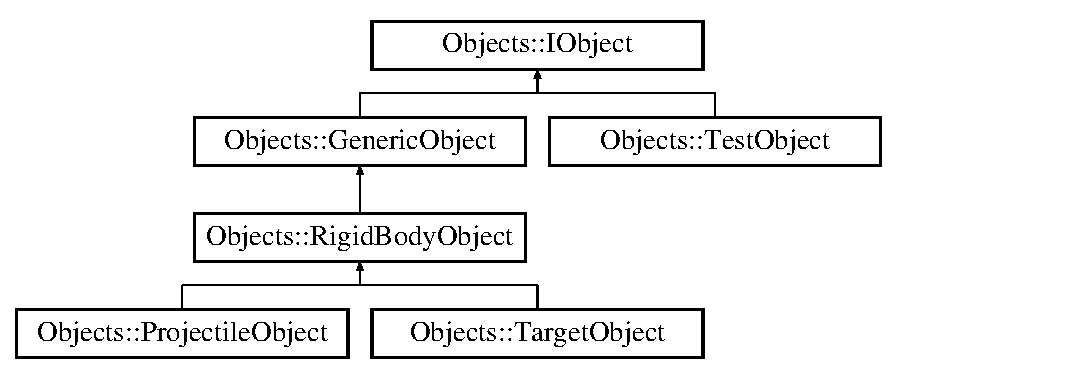
\includegraphics[height=4.000000cm]{class_objects_1_1_i_object}
\end{center}
\end{figure}
\subsection*{Public Member Functions}
\begin{DoxyCompactItemize}
\item 
\hypertarget{class_objects_1_1_i_object_a932898790e2babe2ba4c95c561f862e8}{virtual void \hyperlink{class_objects_1_1_i_object_a932898790e2babe2ba4c95c561f862e8}{initialise} ()=0}\label{class_objects_1_1_i_object_a932898790e2babe2ba4c95c561f862e8}

\begin{DoxyCompactList}\small\item\em Initialises this object. \end{DoxyCompactList}\item 
virtual void \hyperlink{class_objects_1_1_i_object_a616e6befc5fbdca47155b1b56d0e0fc0}{update} (float delta\-Time)
\begin{DoxyCompactList}\small\item\em Updates the given delta\-Time. \end{DoxyCompactList}\item 
void \hyperlink{class_objects_1_1_i_object_abb8bb5097d1600f4e5d0aea2cd148247}{set\-Mesh\-File} (std\-::string filename)
\begin{DoxyCompactList}\small\item\em Sets mesh file. \end{DoxyCompactList}\item 
\hypertarget{class_objects_1_1_i_object_a8043777b3c370b2f422319a552373bc0}{void \hyperlink{class_objects_1_1_i_object_a8043777b3c370b2f422319a552373bc0}{Make\-Collision\-Object} ()}\label{class_objects_1_1_i_object_a8043777b3c370b2f422319a552373bc0}

\begin{DoxyCompactList}\small\item\em Makes collision object. \end{DoxyCompactList}\item 
\hypertarget{class_objects_1_1_i_object_a8e42f185ed7088ed7b4143f9dee1b55a}{void \hyperlink{class_objects_1_1_i_object_a8e42f185ed7088ed7b4143f9dee1b55a}{Make\-Sphere\-Collision\-Object} ()}\label{class_objects_1_1_i_object_a8e42f185ed7088ed7b4143f9dee1b55a}

\begin{DoxyCompactList}\small\item\em Makes sphere collision object. \end{DoxyCompactList}\item 
\hypertarget{class_objects_1_1_i_object_a8a0f5bc968be8a37a746e8079333b0f9}{void \hyperlink{class_objects_1_1_i_object_a8a0f5bc968be8a37a746e8079333b0f9}{Make\-Box\-Collision\-Object} ()}\label{class_objects_1_1_i_object_a8a0f5bc968be8a37a746e8079333b0f9}

\begin{DoxyCompactList}\small\item\em Makes box collision object. \end{DoxyCompactList}\item 
Ogre\-::\-Vector3 \hyperlink{class_objects_1_1_i_object_ae395cf4191bf916973860106b0816c66}{get\-Position} ()
\begin{DoxyCompactList}\small\item\em Gets the position. \end{DoxyCompactList}\item 
void \hyperlink{class_objects_1_1_i_object_a37e429804be393d3b677f2cff2540073}{set\-Position} (Ogre\-::\-Vector3 pos)
\begin{DoxyCompactList}\small\item\em Sets a position. \end{DoxyCompactList}\item 
void \hyperlink{class_objects_1_1_i_object_abf79e6a85faa05adbba1f1cbc83c3564}{change\-Position} (Ogre\-::\-Vector3 pos)
\begin{DoxyCompactList}\small\item\em Change position. \end{DoxyCompactList}\item 
Ogre\-::\-Quaternion \hyperlink{class_objects_1_1_i_object_aff14fa622a7155a324dca06b5fb9b22f}{get\-Orientation} () const 
\begin{DoxyCompactList}\small\item\em Gets the orientation. \end{DoxyCompactList}\item 
Ogre\-::\-Vector3 \hyperlink{class_objects_1_1_i_object_a0cf4689f31dc6d9bd02b0b94537c8086}{get\-Rotation} () const 
\begin{DoxyCompactList}\small\item\em Gets the rotation. \end{DoxyCompactList}\item 
void \hyperlink{class_objects_1_1_i_object_a310aa6d7062af232279b4594c10e415b}{set\-Orientation} (Ogre\-::\-Quaternion rot)
\begin{DoxyCompactList}\small\item\em Sets an orientation. \end{DoxyCompactList}\item 
void \hyperlink{class_objects_1_1_i_object_a20c88273ac16887e388b8b1c3a872d48}{rotate\-By\-Vector} (Ogre\-::\-Vector3 \&rot, float scale=1.\-0f)
\begin{DoxyCompactList}\small\item\em Rotate by vector. \end{DoxyCompactList}\item 
void \hyperlink{class_objects_1_1_i_object_accebddb15710d11fea7b25f0c77aeab0}{set\-Yaw} (float angle)
\begin{DoxyCompactList}\small\item\em Sets a yaw. \end{DoxyCompactList}\item 
void \hyperlink{class_objects_1_1_i_object_a2b67f17e64732f0c7c984414a32d1f64}{set\-Pitch} (float angle)
\begin{DoxyCompactList}\small\item\em Sets a pitch. \end{DoxyCompactList}\item 
void \hyperlink{class_objects_1_1_i_object_aba95ce780536135ac15eb6bf87098ea0}{set\-Roll} (float angle)
\begin{DoxyCompactList}\small\item\em Sets a roll. \end{DoxyCompactList}\item 
void \hyperlink{class_objects_1_1_i_object_a3f67350d8eb911ce44814f3a109cf273}{set\-Scale} (float x, float y, float z)
\begin{DoxyCompactList}\small\item\em Sets a scale. \end{DoxyCompactList}\item 
void \hyperlink{class_objects_1_1_i_object_a688a2ba3aa58342ff006677c4995411b}{set\-Scale} (Ogre\-::\-Vector3 scale)
\begin{DoxyCompactList}\small\item\em Sets a scale. \end{DoxyCompactList}\item 
Ogre\-::\-Vector3 \hyperlink{class_objects_1_1_i_object_ae03ab75fddc9cd990a4a9bf5137cb00f}{get\-Scale} ()
\begin{DoxyCompactList}\small\item\em Gets the scale. \end{DoxyCompactList}\item 
Ogre\-::\-Quaternion \hyperlink{class_objects_1_1_i_object_a8eafa5d8f1638d50de0cdd34d03e4350}{get\-Orientation} ()
\begin{DoxyCompactList}\small\item\em Gets the orientation. \end{DoxyCompactList}\item 
std\-::string \hyperlink{class_objects_1_1_i_object_aea013005572b9493886fc0b4a12d42ba}{get\-Entity\-Name} ()
\begin{DoxyCompactList}\small\item\em Gets entity name. \end{DoxyCompactList}\item 
Ogre\-::\-Entity $\ast$ \hyperlink{class_objects_1_1_i_object_a5ce456cbcf26b929e255da515c5b37a9}{get\-Entity} ()
\begin{DoxyCompactList}\small\item\em Gets the entity. \end{DoxyCompactList}\item 
std\-::map$<$ std\-::string, int $>$ $\ast$ \hyperlink{class_objects_1_1_i_object_a22b3acfb9b300a09409ac4c986a434a0}{Get\-Map} ()
\begin{DoxyCompactList}\small\item\em Gets the map. \end{DoxyCompactList}\item 
bool \hyperlink{class_objects_1_1_i_object_abaa11138d53ef4976630589899c73539}{Is\-Interactable} ()
\begin{DoxyCompactList}\small\item\em Query if this object is interactable. \end{DoxyCompactList}\item 
void \hyperlink{class_objects_1_1_i_object_a535d1642eae42de6acba933d142defb1}{Set\-Interactable} (bool set)
\begin{DoxyCompactList}\small\item\em Sets an interactable. \end{DoxyCompactList}\item 
int \hyperlink{class_objects_1_1_i_object_aeb573744a2a56f455d85fc06c7b27e37}{Get\-Affodance} (std\-::string affordance)
\begin{DoxyCompactList}\small\item\em Gets an affodance. \end{DoxyCompactList}\end{DoxyCompactItemize}
\subsection*{Public Attributes}
\begin{DoxyCompactItemize}
\item 
\hypertarget{class_objects_1_1_i_object_ada16f56e05325655d57ad1aaf6cd5bf7}{int {\bfseries A\-I}}\label{class_objects_1_1_i_object_ada16f56e05325655d57ad1aaf6cd5bf7}

\item 
\hypertarget{class_objects_1_1_i_object_abb60f2a9f1a2babcbd055a355284dc87}{std\-::string \hyperlink{class_objects_1_1_i_object_abb60f2a9f1a2babcbd055a355284dc87}{Type}}\label{class_objects_1_1_i_object_abb60f2a9f1a2babcbd055a355284dc87}

\begin{DoxyCompactList}\small\item\em The type. \end{DoxyCompactList}\item 
\hypertarget{class_objects_1_1_i_object_a7812cd5cf46e2c3353fca5118e26d8a2}{int \hyperlink{class_objects_1_1_i_object_a7812cd5cf46e2c3353fca5118e26d8a2}{m\-\_\-id}}\label{class_objects_1_1_i_object_a7812cd5cf46e2c3353fca5118e26d8a2}

\begin{DoxyCompactList}\small\item\em The identifier. \end{DoxyCompactList}\item 
\hypertarget{class_objects_1_1_i_object_a4d222a9eeead55bc074b97372b75d7dd}{std\-::map$<$ std\-::string, int $>$ \hyperlink{class_objects_1_1_i_object_a4d222a9eeead55bc074b97372b75d7dd}{Affordances}}\label{class_objects_1_1_i_object_a4d222a9eeead55bc074b97372b75d7dd}

\begin{DoxyCompactList}\small\item\em The affordances. \end{DoxyCompactList}\item 
\hypertarget{class_objects_1_1_i_object_a98a45fcbb771b4b7aa9e3e517005c89d}{bool \hyperlink{class_objects_1_1_i_object_a98a45fcbb771b4b7aa9e3e517005c89d}{Generic}}\label{class_objects_1_1_i_object_a98a45fcbb771b4b7aa9e3e517005c89d}

\begin{DoxyCompactList}\small\item\em true to generic. \end{DoxyCompactList}\item 
\hypertarget{class_objects_1_1_i_object_acacfe9cceb90229b824063b47efa3171}{bool \hyperlink{class_objects_1_1_i_object_acacfe9cceb90229b824063b47efa3171}{is\-Dynamic}}\label{class_objects_1_1_i_object_acacfe9cceb90229b824063b47efa3171}

\begin{DoxyCompactList}\small\item\em true if this object is dynamic. \end{DoxyCompactList}\end{DoxyCompactItemize}
\subsection*{Protected Member Functions}
\begin{DoxyCompactItemize}
\item 
\hypertarget{class_objects_1_1_i_object_a0a5cb41bb995dcfb01c3880600ae8340}{void \hyperlink{class_objects_1_1_i_object_a0a5cb41bb995dcfb01c3880600ae8340}{load\-Mesh} () const }\label{class_objects_1_1_i_object_a0a5cb41bb995dcfb01c3880600ae8340}

\begin{DoxyCompactList}\small\item\em Loads the mesh. \end{DoxyCompactList}\item 
\hypertarget{class_objects_1_1_i_object_a7bd6a849a416450530b991dfb7068715}{void \hyperlink{class_objects_1_1_i_object_a7bd6a849a416450530b991dfb7068715}{set\-I\-D} ()}\label{class_objects_1_1_i_object_a7bd6a849a416450530b991dfb7068715}

\begin{DoxyCompactList}\small\item\em Sets the identifier. \end{DoxyCompactList}\end{DoxyCompactItemize}
\subsection*{Protected Attributes}
\begin{DoxyCompactItemize}
\item 
\hypertarget{class_objects_1_1_i_object_a946df067938f5708a5fc92a6a3b7de3b}{\hyperlink{class_collision_object}{Collision\-Object} $\ast$ \hyperlink{class_objects_1_1_i_object_a946df067938f5708a5fc92a6a3b7de3b}{Col\-Obj}}\label{class_objects_1_1_i_object_a946df067938f5708a5fc92a6a3b7de3b}

\begin{DoxyCompactList}\small\item\em The col object. \end{DoxyCompactList}\item 
\hypertarget{class_objects_1_1_i_object_a7e8a3b317f3bd294609e7ea2e4915ea2}{Ogre\-::\-Vector3 \hyperlink{class_objects_1_1_i_object_a7e8a3b317f3bd294609e7ea2e4915ea2}{m\-\_\-position}}\label{class_objects_1_1_i_object_a7e8a3b317f3bd294609e7ea2e4915ea2}

\begin{DoxyCompactList}\small\item\em The position. \end{DoxyCompactList}\item 
\hypertarget{class_objects_1_1_i_object_ac3825691191c3b7d577c945c194a6e8a}{Ogre\-::\-Quaternion \hyperlink{class_objects_1_1_i_object_ac3825691191c3b7d577c945c194a6e8a}{m\-\_\-rotation}}\label{class_objects_1_1_i_object_ac3825691191c3b7d577c945c194a6e8a}

\begin{DoxyCompactList}\small\item\em The rotation. \end{DoxyCompactList}\item 
\hypertarget{class_objects_1_1_i_object_a98cc8033a8294ef833156cd3cc354657}{std\-::string \hyperlink{class_objects_1_1_i_object_a98cc8033a8294ef833156cd3cc354657}{m\-\_\-filename}}\label{class_objects_1_1_i_object_a98cc8033a8294ef833156cd3cc354657}

\begin{DoxyCompactList}\small\item\em Filename of the file. \end{DoxyCompactList}\end{DoxyCompactItemize}


\subsection{Detailed Description}
Object. 

\subsection{Member Function Documentation}
\hypertarget{class_objects_1_1_i_object_abf79e6a85faa05adbba1f1cbc83c3564}{\index{Objects\-::\-I\-Object@{Objects\-::\-I\-Object}!change\-Position@{change\-Position}}
\index{change\-Position@{change\-Position}!Objects::IObject@{Objects\-::\-I\-Object}}
\subsubsection[{change\-Position}]{\setlength{\rightskip}{0pt plus 5cm}void Objects\-::\-I\-Object\-::change\-Position (
\begin{DoxyParamCaption}
\item[{Ogre\-::\-Vector3}]{pos}
\end{DoxyParamCaption}
)}}\label{class_objects_1_1_i_object_abf79e6a85faa05adbba1f1cbc83c3564}


Change position. 


\begin{DoxyParams}{Parameters}
{\em pos} & The position. \\
\hline
\end{DoxyParams}
\hypertarget{class_objects_1_1_i_object_aeb573744a2a56f455d85fc06c7b27e37}{\index{Objects\-::\-I\-Object@{Objects\-::\-I\-Object}!Get\-Affodance@{Get\-Affodance}}
\index{Get\-Affodance@{Get\-Affodance}!Objects::IObject@{Objects\-::\-I\-Object}}
\subsubsection[{Get\-Affodance}]{\setlength{\rightskip}{0pt plus 5cm}int Objects\-::\-I\-Object\-::\-Get\-Affodance (
\begin{DoxyParamCaption}
\item[{std\-::string}]{affordance}
\end{DoxyParamCaption}
)}}\label{class_objects_1_1_i_object_aeb573744a2a56f455d85fc06c7b27e37}


Gets an affodance. 


\begin{DoxyParams}{Parameters}
{\em affordance} & The affordance.\\
\hline
\end{DoxyParams}
\begin{DoxyReturn}{Returns}
The affodance. 
\end{DoxyReturn}
\hypertarget{class_objects_1_1_i_object_a5ce456cbcf26b929e255da515c5b37a9}{\index{Objects\-::\-I\-Object@{Objects\-::\-I\-Object}!get\-Entity@{get\-Entity}}
\index{get\-Entity@{get\-Entity}!Objects::IObject@{Objects\-::\-I\-Object}}
\subsubsection[{get\-Entity}]{\setlength{\rightskip}{0pt plus 5cm}Ogre\-::\-Entity $\ast$ Objects\-::\-I\-Object\-::get\-Entity (
\begin{DoxyParamCaption}
{}
\end{DoxyParamCaption}
)}}\label{class_objects_1_1_i_object_a5ce456cbcf26b929e255da515c5b37a9}


Gets the entity. 

\begin{DoxyReturn}{Returns}
null if it fails, else the entity. 
\end{DoxyReturn}
\hypertarget{class_objects_1_1_i_object_aea013005572b9493886fc0b4a12d42ba}{\index{Objects\-::\-I\-Object@{Objects\-::\-I\-Object}!get\-Entity\-Name@{get\-Entity\-Name}}
\index{get\-Entity\-Name@{get\-Entity\-Name}!Objects::IObject@{Objects\-::\-I\-Object}}
\subsubsection[{get\-Entity\-Name}]{\setlength{\rightskip}{0pt plus 5cm}std\-::string Objects\-::\-I\-Object\-::get\-Entity\-Name (
\begin{DoxyParamCaption}
{}
\end{DoxyParamCaption}
)}}\label{class_objects_1_1_i_object_aea013005572b9493886fc0b4a12d42ba}


Gets entity name. 

\begin{DoxyReturn}{Returns}
The entity name. 
\end{DoxyReturn}
\hypertarget{class_objects_1_1_i_object_a22b3acfb9b300a09409ac4c986a434a0}{\index{Objects\-::\-I\-Object@{Objects\-::\-I\-Object}!Get\-Map@{Get\-Map}}
\index{Get\-Map@{Get\-Map}!Objects::IObject@{Objects\-::\-I\-Object}}
\subsubsection[{Get\-Map}]{\setlength{\rightskip}{0pt plus 5cm}std\-::map$<$ std\-::string, int $>$ $\ast$ Objects\-::\-I\-Object\-::\-Get\-Map (
\begin{DoxyParamCaption}
{}
\end{DoxyParamCaption}
)}}\label{class_objects_1_1_i_object_a22b3acfb9b300a09409ac4c986a434a0}


Gets the map. 

\begin{DoxyReturn}{Returns}
null if it fails, else the map. 
\end{DoxyReturn}
\hypertarget{class_objects_1_1_i_object_aff14fa622a7155a324dca06b5fb9b22f}{\index{Objects\-::\-I\-Object@{Objects\-::\-I\-Object}!get\-Orientation@{get\-Orientation}}
\index{get\-Orientation@{get\-Orientation}!Objects::IObject@{Objects\-::\-I\-Object}}
\subsubsection[{get\-Orientation}]{\setlength{\rightskip}{0pt plus 5cm}Ogre\-::\-Quaternion Objects\-::\-I\-Object\-::get\-Orientation (
\begin{DoxyParamCaption}
{}
\end{DoxyParamCaption}
) const}}\label{class_objects_1_1_i_object_aff14fa622a7155a324dca06b5fb9b22f}


Gets the orientation. 

\begin{DoxyReturn}{Returns}
The orientation. 
\end{DoxyReturn}
\hypertarget{class_objects_1_1_i_object_a8eafa5d8f1638d50de0cdd34d03e4350}{\index{Objects\-::\-I\-Object@{Objects\-::\-I\-Object}!get\-Orientation@{get\-Orientation}}
\index{get\-Orientation@{get\-Orientation}!Objects::IObject@{Objects\-::\-I\-Object}}
\subsubsection[{get\-Orientation}]{\setlength{\rightskip}{0pt plus 5cm}Ogre\-::\-Quaternion Objects\-::\-I\-Object\-::get\-Orientation (
\begin{DoxyParamCaption}
{}
\end{DoxyParamCaption}
)}}\label{class_objects_1_1_i_object_a8eafa5d8f1638d50de0cdd34d03e4350}


Gets the orientation. 

\begin{DoxyReturn}{Returns}
The orientation. 
\end{DoxyReturn}
\hypertarget{class_objects_1_1_i_object_ae395cf4191bf916973860106b0816c66}{\index{Objects\-::\-I\-Object@{Objects\-::\-I\-Object}!get\-Position@{get\-Position}}
\index{get\-Position@{get\-Position}!Objects::IObject@{Objects\-::\-I\-Object}}
\subsubsection[{get\-Position}]{\setlength{\rightskip}{0pt plus 5cm}Ogre\-::\-Vector3 Objects\-::\-I\-Object\-::get\-Position (
\begin{DoxyParamCaption}
{}
\end{DoxyParamCaption}
)}}\label{class_objects_1_1_i_object_ae395cf4191bf916973860106b0816c66}


Gets the position. 

\begin{DoxyReturn}{Returns}
The position. 
\end{DoxyReturn}
\hypertarget{class_objects_1_1_i_object_a0cf4689f31dc6d9bd02b0b94537c8086}{\index{Objects\-::\-I\-Object@{Objects\-::\-I\-Object}!get\-Rotation@{get\-Rotation}}
\index{get\-Rotation@{get\-Rotation}!Objects::IObject@{Objects\-::\-I\-Object}}
\subsubsection[{get\-Rotation}]{\setlength{\rightskip}{0pt plus 5cm}Ogre\-::\-Vector3 Objects\-::\-I\-Object\-::get\-Rotation (
\begin{DoxyParamCaption}
{}
\end{DoxyParamCaption}
) const}}\label{class_objects_1_1_i_object_a0cf4689f31dc6d9bd02b0b94537c8086}


Gets the rotation. 

\begin{DoxyReturn}{Returns}
The rotation. 
\end{DoxyReturn}
\hypertarget{class_objects_1_1_i_object_ae03ab75fddc9cd990a4a9bf5137cb00f}{\index{Objects\-::\-I\-Object@{Objects\-::\-I\-Object}!get\-Scale@{get\-Scale}}
\index{get\-Scale@{get\-Scale}!Objects::IObject@{Objects\-::\-I\-Object}}
\subsubsection[{get\-Scale}]{\setlength{\rightskip}{0pt plus 5cm}Ogre\-::\-Vector3 Objects\-::\-I\-Object\-::get\-Scale (
\begin{DoxyParamCaption}
{}
\end{DoxyParamCaption}
)}}\label{class_objects_1_1_i_object_ae03ab75fddc9cd990a4a9bf5137cb00f}


Gets the scale. 

\begin{DoxyReturn}{Returns}
The scale. 
\end{DoxyReturn}
\hypertarget{class_objects_1_1_i_object_abaa11138d53ef4976630589899c73539}{\index{Objects\-::\-I\-Object@{Objects\-::\-I\-Object}!Is\-Interactable@{Is\-Interactable}}
\index{Is\-Interactable@{Is\-Interactable}!Objects::IObject@{Objects\-::\-I\-Object}}
\subsubsection[{Is\-Interactable}]{\setlength{\rightskip}{0pt plus 5cm}bool Objects\-::\-I\-Object\-::\-Is\-Interactable (
\begin{DoxyParamCaption}
{}
\end{DoxyParamCaption}
)}}\label{class_objects_1_1_i_object_abaa11138d53ef4976630589899c73539}


Query if this object is interactable. 

\begin{DoxyReturn}{Returns}
true if interactable, false if not. 
\end{DoxyReturn}
\hypertarget{class_objects_1_1_i_object_a20c88273ac16887e388b8b1c3a872d48}{\index{Objects\-::\-I\-Object@{Objects\-::\-I\-Object}!rotate\-By\-Vector@{rotate\-By\-Vector}}
\index{rotate\-By\-Vector@{rotate\-By\-Vector}!Objects::IObject@{Objects\-::\-I\-Object}}
\subsubsection[{rotate\-By\-Vector}]{\setlength{\rightskip}{0pt plus 5cm}void Objects\-::\-I\-Object\-::rotate\-By\-Vector (
\begin{DoxyParamCaption}
\item[{Ogre\-::\-Vector3 \&}]{rot, }
\item[{float}]{scale = {\ttfamily 1.0f}}
\end{DoxyParamCaption}
)}}\label{class_objects_1_1_i_object_a20c88273ac16887e388b8b1c3a872d48}


Rotate by vector. 


\begin{DoxyParams}[1]{Parameters}
\mbox{\tt in,out}  & {\em rot} & The rot. \\
\hline
 & {\em scale} & (optional) the scale. \\
\hline
\end{DoxyParams}
\hypertarget{class_objects_1_1_i_object_a535d1642eae42de6acba933d142defb1}{\index{Objects\-::\-I\-Object@{Objects\-::\-I\-Object}!Set\-Interactable@{Set\-Interactable}}
\index{Set\-Interactable@{Set\-Interactable}!Objects::IObject@{Objects\-::\-I\-Object}}
\subsubsection[{Set\-Interactable}]{\setlength{\rightskip}{0pt plus 5cm}void Objects\-::\-I\-Object\-::\-Set\-Interactable (
\begin{DoxyParamCaption}
\item[{bool}]{set}
\end{DoxyParamCaption}
)\hspace{0.3cm}{\ttfamily [inline]}}}\label{class_objects_1_1_i_object_a535d1642eae42de6acba933d142defb1}


Sets an interactable. 


\begin{DoxyParams}{Parameters}
{\em set} & true to set. \\
\hline
\end{DoxyParams}
\hypertarget{class_objects_1_1_i_object_abb8bb5097d1600f4e5d0aea2cd148247}{\index{Objects\-::\-I\-Object@{Objects\-::\-I\-Object}!set\-Mesh\-File@{set\-Mesh\-File}}
\index{set\-Mesh\-File@{set\-Mesh\-File}!Objects::IObject@{Objects\-::\-I\-Object}}
\subsubsection[{set\-Mesh\-File}]{\setlength{\rightskip}{0pt plus 5cm}void Objects\-::\-I\-Object\-::set\-Mesh\-File (
\begin{DoxyParamCaption}
\item[{std\-::string}]{filename}
\end{DoxyParamCaption}
)}}\label{class_objects_1_1_i_object_abb8bb5097d1600f4e5d0aea2cd148247}


Sets mesh file. 


\begin{DoxyParams}{Parameters}
{\em filename} & Filename of the file. \\
\hline
\end{DoxyParams}
\hypertarget{class_objects_1_1_i_object_a310aa6d7062af232279b4594c10e415b}{\index{Objects\-::\-I\-Object@{Objects\-::\-I\-Object}!set\-Orientation@{set\-Orientation}}
\index{set\-Orientation@{set\-Orientation}!Objects::IObject@{Objects\-::\-I\-Object}}
\subsubsection[{set\-Orientation}]{\setlength{\rightskip}{0pt plus 5cm}void Objects\-::\-I\-Object\-::set\-Orientation (
\begin{DoxyParamCaption}
\item[{Ogre\-::\-Quaternion}]{rot}
\end{DoxyParamCaption}
)}}\label{class_objects_1_1_i_object_a310aa6d7062af232279b4594c10e415b}


Sets an orientation. 


\begin{DoxyParams}{Parameters}
{\em rot} & The rot. \\
\hline
\end{DoxyParams}
\hypertarget{class_objects_1_1_i_object_a2b67f17e64732f0c7c984414a32d1f64}{\index{Objects\-::\-I\-Object@{Objects\-::\-I\-Object}!set\-Pitch@{set\-Pitch}}
\index{set\-Pitch@{set\-Pitch}!Objects::IObject@{Objects\-::\-I\-Object}}
\subsubsection[{set\-Pitch}]{\setlength{\rightskip}{0pt plus 5cm}void Objects\-::\-I\-Object\-::set\-Pitch (
\begin{DoxyParamCaption}
\item[{float}]{angle}
\end{DoxyParamCaption}
)}}\label{class_objects_1_1_i_object_a2b67f17e64732f0c7c984414a32d1f64}


Sets a pitch. 


\begin{DoxyParams}{Parameters}
{\em angle} & The angle. \\
\hline
\end{DoxyParams}
\hypertarget{class_objects_1_1_i_object_a37e429804be393d3b677f2cff2540073}{\index{Objects\-::\-I\-Object@{Objects\-::\-I\-Object}!set\-Position@{set\-Position}}
\index{set\-Position@{set\-Position}!Objects::IObject@{Objects\-::\-I\-Object}}
\subsubsection[{set\-Position}]{\setlength{\rightskip}{0pt plus 5cm}void Objects\-::\-I\-Object\-::set\-Position (
\begin{DoxyParamCaption}
\item[{Ogre\-::\-Vector3}]{pos}
\end{DoxyParamCaption}
)}}\label{class_objects_1_1_i_object_a37e429804be393d3b677f2cff2540073}


Sets a position. 


\begin{DoxyParams}{Parameters}
{\em pos} & The position. \\
\hline
\end{DoxyParams}
\hypertarget{class_objects_1_1_i_object_aba95ce780536135ac15eb6bf87098ea0}{\index{Objects\-::\-I\-Object@{Objects\-::\-I\-Object}!set\-Roll@{set\-Roll}}
\index{set\-Roll@{set\-Roll}!Objects::IObject@{Objects\-::\-I\-Object}}
\subsubsection[{set\-Roll}]{\setlength{\rightskip}{0pt plus 5cm}void Objects\-::\-I\-Object\-::set\-Roll (
\begin{DoxyParamCaption}
\item[{float}]{angle}
\end{DoxyParamCaption}
)}}\label{class_objects_1_1_i_object_aba95ce780536135ac15eb6bf87098ea0}


Sets a roll. 


\begin{DoxyParams}{Parameters}
{\em angle} & The angle. \\
\hline
\end{DoxyParams}
\hypertarget{class_objects_1_1_i_object_a3f67350d8eb911ce44814f3a109cf273}{\index{Objects\-::\-I\-Object@{Objects\-::\-I\-Object}!set\-Scale@{set\-Scale}}
\index{set\-Scale@{set\-Scale}!Objects::IObject@{Objects\-::\-I\-Object}}
\subsubsection[{set\-Scale}]{\setlength{\rightskip}{0pt plus 5cm}void Objects\-::\-I\-Object\-::set\-Scale (
\begin{DoxyParamCaption}
\item[{float}]{x, }
\item[{float}]{y, }
\item[{float}]{z}
\end{DoxyParamCaption}
)}}\label{class_objects_1_1_i_object_a3f67350d8eb911ce44814f3a109cf273}


Sets a scale. 


\begin{DoxyParams}{Parameters}
{\em x} & The x coordinate. \\
\hline
{\em y} & The y coordinate. \\
\hline
{\em z} & The z coordinate. \\
\hline
\end{DoxyParams}
\hypertarget{class_objects_1_1_i_object_a688a2ba3aa58342ff006677c4995411b}{\index{Objects\-::\-I\-Object@{Objects\-::\-I\-Object}!set\-Scale@{set\-Scale}}
\index{set\-Scale@{set\-Scale}!Objects::IObject@{Objects\-::\-I\-Object}}
\subsubsection[{set\-Scale}]{\setlength{\rightskip}{0pt plus 5cm}void Objects\-::\-I\-Object\-::set\-Scale (
\begin{DoxyParamCaption}
\item[{Ogre\-::\-Vector3}]{scale}
\end{DoxyParamCaption}
)}}\label{class_objects_1_1_i_object_a688a2ba3aa58342ff006677c4995411b}


Sets a scale. 


\begin{DoxyParams}{Parameters}
{\em scale} & The scale. \\
\hline
\end{DoxyParams}
\hypertarget{class_objects_1_1_i_object_accebddb15710d11fea7b25f0c77aeab0}{\index{Objects\-::\-I\-Object@{Objects\-::\-I\-Object}!set\-Yaw@{set\-Yaw}}
\index{set\-Yaw@{set\-Yaw}!Objects::IObject@{Objects\-::\-I\-Object}}
\subsubsection[{set\-Yaw}]{\setlength{\rightskip}{0pt plus 5cm}void Objects\-::\-I\-Object\-::set\-Yaw (
\begin{DoxyParamCaption}
\item[{float}]{angle}
\end{DoxyParamCaption}
)}}\label{class_objects_1_1_i_object_accebddb15710d11fea7b25f0c77aeab0}


Sets a yaw. 


\begin{DoxyParams}{Parameters}
{\em angle} & The angle. \\
\hline
\end{DoxyParams}
\hypertarget{class_objects_1_1_i_object_a616e6befc5fbdca47155b1b56d0e0fc0}{\index{Objects\-::\-I\-Object@{Objects\-::\-I\-Object}!update@{update}}
\index{update@{update}!Objects::IObject@{Objects\-::\-I\-Object}}
\subsubsection[{update}]{\setlength{\rightskip}{0pt plus 5cm}void Objects\-::\-I\-Object\-::update (
\begin{DoxyParamCaption}
\item[{float}]{delta\-Time}
\end{DoxyParamCaption}
)\hspace{0.3cm}{\ttfamily [virtual]}}}\label{class_objects_1_1_i_object_a616e6befc5fbdca47155b1b56d0e0fc0}


Updates the given delta\-Time. 


\begin{DoxyParams}{Parameters}
{\em delta\-Time} & Time of the delta. \\
\hline
\end{DoxyParams}


Reimplemented in \hyperlink{class_objects_1_1_generic_object_a57c85bdf2ceb1ffa1b85ec3aa51a631d}{Objects\-::\-Generic\-Object}, \hyperlink{class_objects_1_1_rigid_body_object_a478edcbc5820722a9641fdcd07b402bb}{Objects\-::\-Rigid\-Body\-Object}, \hyperlink{class_objects_1_1_target_object_a46b8163c5921925aa6d95fc0e99ce011}{Objects\-::\-Target\-Object}, \hyperlink{class_objects_1_1_projectile_object_ae8cb3b7f7a9f5b921b043a58e9e355dc}{Objects\-::\-Projectile\-Object}, and \hyperlink{class_objects_1_1_test_object_a5df5df31f7f1233cd991d200ecac7205}{Objects\-::\-Test\-Object}.



The documentation for this class was generated from the following files\-:\begin{DoxyCompactItemize}
\item 
A\-:/\-I\-T/\-Git\-Hub/\-I\-C\-T312/source/ogregraphics/\hyperlink{_i_object_8h}{I\-Object.\-h}\item 
A\-:/\-I\-T/\-Git\-Hub/\-I\-C\-T312/source/ogregraphics/I\-Object.\-cpp\end{DoxyCompactItemize}

\hypertarget{class_scenes_1_1_i_scene}{\section{Scenes\-:\-:I\-Scene Class Reference}
\label{class_scenes_1_1_i_scene}\index{Scenes\-::\-I\-Scene@{Scenes\-::\-I\-Scene}}
}


Scene interface including scene initialisation, updating and actions when the scene is exited.  




{\ttfamily \#include $<$I\-Scene.\-h$>$}

Inheritance diagram for Scenes\-:\-:I\-Scene\-:\begin{figure}[H]
\begin{center}
\leavevmode
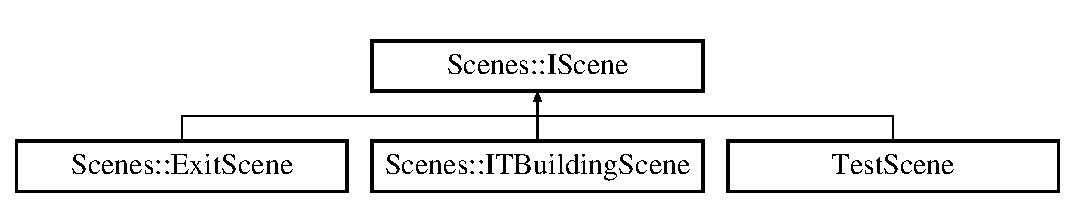
\includegraphics[height=2.000000cm]{class_scenes_1_1_i_scene}
\end{center}
\end{figure}
\subsection*{Public Member Functions}
\begin{DoxyCompactItemize}
\item 
\hypertarget{class_scenes_1_1_i_scene_a4f3faceff8b6ce9209f8268975efe752}{virtual void \hyperlink{class_scenes_1_1_i_scene_a4f3faceff8b6ce9209f8268975efe752}{initialise} ()=0}\label{class_scenes_1_1_i_scene_a4f3faceff8b6ce9209f8268975efe752}

\begin{DoxyCompactList}\small\item\em Initialises the scene. \end{DoxyCompactList}\item 
virtual void \hyperlink{class_scenes_1_1_i_scene_acb97c42a9a93ce1b3d0b800bda680935}{update} (float delta\-Time)
\begin{DoxyCompactList}\small\item\em Updates the scene given the change in time from one frame to another. \end{DoxyCompactList}\item 
\hypertarget{class_scenes_1_1_i_scene_a3abd220af7da336ec3b1c75444254fbc}{virtual void \hyperlink{class_scenes_1_1_i_scene_a3abd220af7da336ec3b1c75444254fbc}{on\-Exit} ()=0}\label{class_scenes_1_1_i_scene_a3abd220af7da336ec3b1c75444254fbc}

\begin{DoxyCompactList}\small\item\em Called upon the scene being closed. \end{DoxyCompactList}\item 
\hypertarget{class_scenes_1_1_i_scene_ac04de08bb2b1af96e8fde0e1b86255ad}{void {\bfseries add\-Object} (std\-::string identifier, \hyperlink{class_objects_1_1_i_object}{Objects\-::\-I\-Object} $\ast$object)}\label{class_scenes_1_1_i_scene_ac04de08bb2b1af96e8fde0e1b86255ad}

\item 
\hypertarget{class_scenes_1_1_i_scene_af8f4f0a6918286c669fc309fe8c6208d}{void {\bfseries remove\-Object} (std\-::string identifier)}\label{class_scenes_1_1_i_scene_af8f4f0a6918286c669fc309fe8c6208d}

\item 
\hypertarget{class_scenes_1_1_i_scene_a7028f9be6feec9aeedc677a8b321bf42}{\hyperlink{class_objects_1_1_i_object}{Objects\-::\-I\-Object} $\ast$ {\bfseries get\-Object} (std\-::string identifier)}\label{class_scenes_1_1_i_scene_a7028f9be6feec9aeedc677a8b321bf42}

\end{DoxyCompactItemize}


\subsection{Detailed Description}
Scene interface including scene initialisation, updating and actions when the scene is exited. 

\begin{DoxyAuthor}{Author}
Timothy Veletta 
\end{DoxyAuthor}
\begin{DoxyDate}{Date}
15/08/13 
\end{DoxyDate}


\subsection{Member Function Documentation}
\hypertarget{class_scenes_1_1_i_scene_acb97c42a9a93ce1b3d0b800bda680935}{\index{Scenes\-::\-I\-Scene@{Scenes\-::\-I\-Scene}!update@{update}}
\index{update@{update}!Scenes::IScene@{Scenes\-::\-I\-Scene}}
\subsubsection[{update}]{\setlength{\rightskip}{0pt plus 5cm}void Scenes\-::\-I\-Scene\-::update (
\begin{DoxyParamCaption}
\item[{float}]{delta\-Time}
\end{DoxyParamCaption}
)\hspace{0.3cm}{\ttfamily [virtual]}}}\label{class_scenes_1_1_i_scene_acb97c42a9a93ce1b3d0b800bda680935}


Updates the scene given the change in time from one frame to another. 


\begin{DoxyParams}{Parameters}
{\em delta\-Time} & The change in time from one frame to another. \\
\hline
\end{DoxyParams}


Reimplemented in \hyperlink{class_test_scene_ad42240fabf5883d481191871cc91c5c3}{Test\-Scene}, \hyperlink{class_scenes_1_1_i_t_building_scene_acc67b30b6a5f3d47b55c1d7366f2668c}{Scenes\-::\-I\-T\-Building\-Scene}, and \hyperlink{class_scenes_1_1_exit_scene_ab252f553afc98976f67a0e2c330caed4}{Scenes\-::\-Exit\-Scene}.



The documentation for this class was generated from the following files\-:\begin{DoxyCompactItemize}
\item 
A\-:/\-I\-T/\-Git\-Hub/\-I\-C\-T312/source/ogregraphics/I\-Scene.\-h\item 
A\-:/\-I\-T/\-Git\-Hub/\-I\-C\-T312/source/ogregraphics/I\-Scene.\-cpp\end{DoxyCompactItemize}

\hypertarget{class_scenes_1_1_i_t_building_scene}{\section{Scenes\-:\-:I\-T\-Building\-Scene Class Reference}
\label{class_scenes_1_1_i_t_building_scene}\index{Scenes\-::\-I\-T\-Building\-Scene@{Scenes\-::\-I\-T\-Building\-Scene}}
}


Iterator building scene.  




{\ttfamily \#include $<$I\-T\-Building\-Scene.\-h$>$}

Inheritance diagram for Scenes\-:\-:I\-T\-Building\-Scene\-:\begin{figure}[H]
\begin{center}
\leavevmode
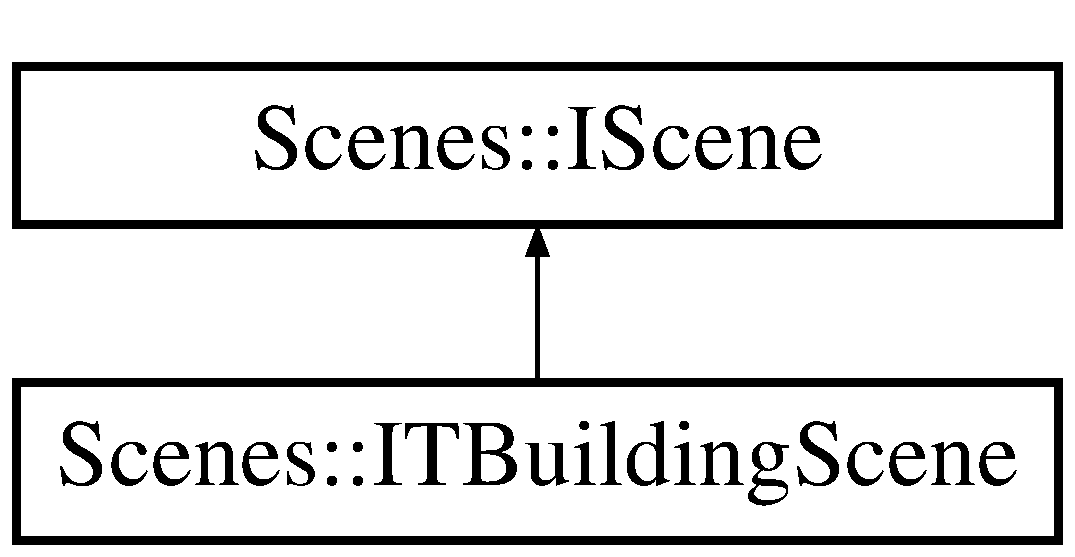
\includegraphics[height=2.000000cm]{class_scenes_1_1_i_t_building_scene}
\end{center}
\end{figure}
\subsection*{Public Member Functions}
\begin{DoxyCompactItemize}
\item 
\hypertarget{class_scenes_1_1_i_t_building_scene_a2585d014b85892ceaad3c933ddb692ab}{virtual void \hyperlink{class_scenes_1_1_i_t_building_scene_a2585d014b85892ceaad3c933ddb692ab}{initialise} ()}\label{class_scenes_1_1_i_t_building_scene_a2585d014b85892ceaad3c933ddb692ab}

\begin{DoxyCompactList}\small\item\em Initialises this object. \end{DoxyCompactList}\item 
virtual void \hyperlink{class_scenes_1_1_i_t_building_scene_acc67b30b6a5f3d47b55c1d7366f2668c}{update} (float delta\-Time)
\begin{DoxyCompactList}\small\item\em Updates the given delta\-Time. \end{DoxyCompactList}\item 
\hypertarget{class_scenes_1_1_i_t_building_scene_a6009eb7e3ef0715b898157c3b29b9298}{virtual void \hyperlink{class_scenes_1_1_i_t_building_scene_a6009eb7e3ef0715b898157c3b29b9298}{on\-Exit} ()}\label{class_scenes_1_1_i_t_building_scene_a6009eb7e3ef0715b898157c3b29b9298}

\begin{DoxyCompactList}\small\item\em Executes the exit action. \end{DoxyCompactList}\end{DoxyCompactItemize}


\subsection{Detailed Description}
Iterator building scene. 

\subsection{Member Function Documentation}
\hypertarget{class_scenes_1_1_i_t_building_scene_acc67b30b6a5f3d47b55c1d7366f2668c}{\index{Scenes\-::\-I\-T\-Building\-Scene@{Scenes\-::\-I\-T\-Building\-Scene}!update@{update}}
\index{update@{update}!Scenes::ITBuildingScene@{Scenes\-::\-I\-T\-Building\-Scene}}
\subsubsection[{update}]{\setlength{\rightskip}{0pt plus 5cm}void Scenes\-::\-I\-T\-Building\-Scene\-::update (
\begin{DoxyParamCaption}
\item[{float}]{delta\-Time}
\end{DoxyParamCaption}
)\hspace{0.3cm}{\ttfamily [virtual]}}}\label{class_scenes_1_1_i_t_building_scene_acc67b30b6a5f3d47b55c1d7366f2668c}


Updates the given delta\-Time. 


\begin{DoxyParams}{Parameters}
{\em delta\-Time} & Time of the delta. \\
\hline
\end{DoxyParams}


Reimplemented from \hyperlink{class_scenes_1_1_i_scene_acb97c42a9a93ce1b3d0b800bda680935}{Scenes\-::\-I\-Scene}.



The documentation for this class was generated from the following files\-:\begin{DoxyCompactItemize}
\item 
A\-:/\-I\-T/\-Git\-Hub/\-I\-C\-T312/source/ogregraphics/\hyperlink{_i_t_building_scene_8h}{I\-T\-Building\-Scene.\-h}\item 
A\-:/\-I\-T/\-Git\-Hub/\-I\-C\-T312/source/ogregraphics/I\-T\-Building\-Scene.\-cpp\end{DoxyCompactItemize}

\hypertarget{class_item_store}{\section{Item\-Store Class Reference}
\label{class_item_store}\index{Item\-Store@{Item\-Store}}
}
\subsection*{Public Member Functions}
\begin{DoxyCompactItemize}
\item 
\hypertarget{class_item_store_a1d378aa7abf88f7cbc121375e7ca5031}{\hyperlink{class_objects_1_1_i_object}{Objects\-::\-I\-Object} $\ast$ {\bfseries Check\-Vector} (std\-::vector$<$ \hyperlink{class_objects_1_1_i_object}{Objects\-::\-I\-Object} $\ast$ $>$ vec, Ogre\-::\-Vector3 pos, std\-::string affordance, int min)}\label{class_item_store_a1d378aa7abf88f7cbc121375e7ca5031}

\item 
\hypertarget{class_item_store_aed446ce89416e3f01d68f70680781e9b}{void {\bfseries Add\-Object} (\hyperlink{class_objects_1_1_i_object}{Objects\-::\-I\-Object} $\ast$obj)}\label{class_item_store_aed446ce89416e3f01d68f70680781e9b}

\item 
\hypertarget{class_item_store_a9998af551c609a934f0d4c0483bf1f75}{\hyperlink{class_objects_1_1_i_object}{Objects\-::\-I\-Object} $\ast$ {\bfseries Get\-Object} (Ogre\-::\-Vector3 pos, std\-::string affordance, int min)}\label{class_item_store_a9998af551c609a934f0d4c0483bf1f75}

\end{DoxyCompactItemize}
\subsection*{Static Public Member Functions}
\begin{DoxyCompactItemize}
\item 
\hypertarget{class_item_store_a23c8996f3a5b116088a954efc6c836b4}{static \hyperlink{class_item_store}{Item\-Store} $\ast$ {\bfseries Instance} ()}\label{class_item_store_a23c8996f3a5b116088a954efc6c836b4}

\end{DoxyCompactItemize}


The documentation for this class was generated from the following files\-:\begin{DoxyCompactItemize}
\item 
A\-:/\-I\-T/\-Git\-Hub/\-I\-C\-T312/source/ogregraphics/Item\-Store.\-h\item 
A\-:/\-I\-T/\-Git\-Hub/\-I\-C\-T312/source/ogregraphics/Item\-Store.\-cpp\end{DoxyCompactItemize}

\hypertarget{struct_ico_sphere_1_1_line_indices}{\section{Ico\-Sphere\-:\-:Line\-Indices Struct Reference}
\label{struct_ico_sphere_1_1_line_indices}\index{Ico\-Sphere\-::\-Line\-Indices@{Ico\-Sphere\-::\-Line\-Indices}}
}
\subsection*{Public Member Functions}
\begin{DoxyCompactItemize}
\item 
\hypertarget{struct_ico_sphere_1_1_line_indices_a5cac383947767b253f73b4ab8b25c4dc}{{\bfseries Line\-Indices} (int \-\_\-v1, int \-\_\-v2)}\label{struct_ico_sphere_1_1_line_indices_a5cac383947767b253f73b4ab8b25c4dc}

\item 
\hypertarget{struct_ico_sphere_1_1_line_indices_a76d97906bf0d50d9ddde77ee8733e0cd}{bool {\bfseries operator==} (const \hyperlink{struct_ico_sphere_1_1_line_indices}{Line\-Indices} \&o) const }\label{struct_ico_sphere_1_1_line_indices_a76d97906bf0d50d9ddde77ee8733e0cd}

\end{DoxyCompactItemize}
\subsection*{Public Attributes}
\begin{DoxyCompactItemize}
\item 
\hypertarget{struct_ico_sphere_1_1_line_indices_a6219c7f06a18aed1ce313af1d8286332}{int {\bfseries v1}}\label{struct_ico_sphere_1_1_line_indices_a6219c7f06a18aed1ce313af1d8286332}

\item 
\hypertarget{struct_ico_sphere_1_1_line_indices_a11e13c571b863b879f212987c831e1ce}{int {\bfseries v2}}\label{struct_ico_sphere_1_1_line_indices_a11e13c571b863b879f212987c831e1ce}

\end{DoxyCompactItemize}


The documentation for this struct was generated from the following file\-:\begin{DoxyCompactItemize}
\item 
A\-:/\-I\-T/\-Git\-Hub/\-I\-C\-T312/source/ogregraphics/Debug\-Drawer.\-h\end{DoxyCompactItemize}

\hypertarget{struct_physics_1_1_manifold}{\section{Physics\-:\-:Manifold Struct Reference}
\label{struct_physics_1_1_manifold}\index{Physics\-::\-Manifold@{Physics\-::\-Manifold}}
}
\subsection*{Public Attributes}
\begin{DoxyCompactItemize}
\item 
\hypertarget{struct_physics_1_1_manifold_a1e30105b5e90089624ff37220d8015d6}{\hyperlink{class_objects_1_1_rigid_body_object}{Objects\-::\-Rigid\-Body\-Object} $\ast$ {\bfseries A}}\label{struct_physics_1_1_manifold_a1e30105b5e90089624ff37220d8015d6}

\item 
\hypertarget{struct_physics_1_1_manifold_aecc0a4e62f050e1a3012438f55f9864e}{\hyperlink{class_objects_1_1_rigid_body_object}{Objects\-::\-Rigid\-Body\-Object} $\ast$ {\bfseries B}}\label{struct_physics_1_1_manifold_aecc0a4e62f050e1a3012438f55f9864e}

\item 
\hypertarget{struct_physics_1_1_manifold_a9527871c4cc0db46cf9ec6700e769681}{Ogre\-::\-Vector3 {\bfseries normal}}\label{struct_physics_1_1_manifold_a9527871c4cc0db46cf9ec6700e769681}

\item 
\hypertarget{struct_physics_1_1_manifold_a053bf2ecd6b844190e405b136fc275f6}{float {\bfseries penetration}}\label{struct_physics_1_1_manifold_a053bf2ecd6b844190e405b136fc275f6}

\item 
\hypertarget{struct_physics_1_1_manifold_a31706b3f6f81123ce5f4bc08c0af0be7}{int {\bfseries num\-Contacts}}\label{struct_physics_1_1_manifold_a31706b3f6f81123ce5f4bc08c0af0be7}

\item 
\hypertarget{struct_physics_1_1_manifold_ae222b04c78b6a07509ed8a4110cd9e97}{Ogre\-::\-Vector3 {\bfseries contacts} \mbox{[}2\mbox{]}}\label{struct_physics_1_1_manifold_ae222b04c78b6a07509ed8a4110cd9e97}

\end{DoxyCompactItemize}


The documentation for this struct was generated from the following file\-:\begin{DoxyCompactItemize}
\item 
A\-:/\-I\-T/\-Git\-Hub/\-I\-C\-T312/source/ogregraphics/Manifold.\-h\end{DoxyCompactItemize}

\hypertarget{class_map_node}{\section{Map\-Node Class Reference}
\label{class_map_node}\index{Map\-Node@{Map\-Node}}
}


This class is a node that can be moved to in the path finding.  




{\ttfamily \#include $<$Map\-Node.\-h$>$}

\subsection*{Public Member Functions}
\begin{DoxyCompactItemize}
\item 
\hyperlink{class_map_node_a19bb10d68456bbfeff7a34432a20cbe2}{Map\-Node} (int ident, Ogre\-::\-Vector3 location)
\begin{DoxyCompactList}\small\item\em Constructor that takes in the location and identifier of the node. \end{DoxyCompactList}\item 
\hyperlink{class_map_node_a3fbf3e9a65ac7ab73bb6fa69c2059462}{Map\-Node} (int ident, Ogre\-::\-Vector3 location, std\-::vector$<$ int $>$ links)
\begin{DoxyCompactList}\small\item\em Constructor takes in the identifier, position and the partners of this node. \end{DoxyCompactList}\item 
int \hyperlink{class_map_node_a340b6649ca8e0b90fe93dcbb327fa789}{Get\-Id} ()
\begin{DoxyCompactList}\small\item\em Gets the identifier. \end{DoxyCompactList}\item 
Ogre\-::\-Vector3 \hyperlink{class_map_node_a9e492d78a10bb716056c5da0897bd27d}{Get\-Location} ()
\begin{DoxyCompactList}\small\item\em Gets the location. \end{DoxyCompactList}\item 
std\-::vector$<$ \hyperlink{class_map_node}{Map\-Node} $\ast$ $>$ $\ast$ \hyperlink{class_map_node_a7b2ba63ca49506414267d972834df68d}{Get\-Partners} ()
\begin{DoxyCompactList}\small\item\em Gets the partners. \end{DoxyCompactList}\item 
\hyperlink{class_map_node}{Map\-Node} $\ast$ \hyperlink{class_map_node_a78608dc546f904c65a1aa0da63eeb331}{Get\-Partner\-By\-Id} (int i)
\begin{DoxyCompactList}\small\item\em Gets partner by identifier. \end{DoxyCompactList}\end{DoxyCompactItemize}
\subsection*{Public Attributes}
\begin{DoxyCompactItemize}
\item 
\hypertarget{class_map_node_a6dce727d54cd79f4f2352771bd6ff20e}{std\-::vector$<$ \hyperlink{class_map_node}{Map\-Node} $\ast$ $>$ \hyperlink{class_map_node_a6dce727d54cd79f4f2352771bd6ff20e}{Partners}}\label{class_map_node_a6dce727d54cd79f4f2352771bd6ff20e}

\begin{DoxyCompactList}\small\item\em A Vector containing pointers to this nodes partners. \end{DoxyCompactList}\end{DoxyCompactItemize}


\subsection{Detailed Description}
This class is a node that can be moved to in the path finding. 

\begin{DoxyAuthor}{Author}
Arran Ford 
\end{DoxyAuthor}
\begin{DoxyDate}{Date}
09/11/2013 
\end{DoxyDate}


\subsection{Constructor \& Destructor Documentation}
\hypertarget{class_map_node_a19bb10d68456bbfeff7a34432a20cbe2}{\index{Map\-Node@{Map\-Node}!Map\-Node@{Map\-Node}}
\index{Map\-Node@{Map\-Node}!MapNode@{Map\-Node}}
\subsubsection[{Map\-Node}]{\setlength{\rightskip}{0pt plus 5cm}Map\-Node\-::\-Map\-Node (
\begin{DoxyParamCaption}
\item[{int}]{ident, }
\item[{Ogre\-::\-Vector3}]{location}
\end{DoxyParamCaption}
)}}\label{class_map_node_a19bb10d68456bbfeff7a34432a20cbe2}


Constructor that takes in the location and identifier of the node. 

\begin{DoxyAuthor}{Author}
Arran Ford 
\end{DoxyAuthor}
\begin{DoxyDate}{Date}
09/11/2013
\end{DoxyDate}

\begin{DoxyParams}{Parameters}
{\em ident} & The identifier. \\
\hline
{\em location} & The location. \\
\hline
\end{DoxyParams}
\hypertarget{class_map_node_a3fbf3e9a65ac7ab73bb6fa69c2059462}{\index{Map\-Node@{Map\-Node}!Map\-Node@{Map\-Node}}
\index{Map\-Node@{Map\-Node}!MapNode@{Map\-Node}}
\subsubsection[{Map\-Node}]{\setlength{\rightskip}{0pt plus 5cm}Map\-Node\-::\-Map\-Node (
\begin{DoxyParamCaption}
\item[{int}]{ident, }
\item[{Ogre\-::\-Vector3}]{location, }
\item[{std\-::vector$<$ int $>$}]{links}
\end{DoxyParamCaption}
)}}\label{class_map_node_a3fbf3e9a65ac7ab73bb6fa69c2059462}


Constructor takes in the identifier, position and the partners of this node. 

\begin{DoxyAuthor}{Author}
Arran Ford 
\end{DoxyAuthor}
\begin{DoxyDate}{Date}
09/11/2013
\end{DoxyDate}

\begin{DoxyParams}{Parameters}
{\em ident} & The identifier. \\
\hline
{\em location} & The location. \\
\hline
{\em links} & The links. \\
\hline
\end{DoxyParams}


\subsection{Member Function Documentation}
\hypertarget{class_map_node_a340b6649ca8e0b90fe93dcbb327fa789}{\index{Map\-Node@{Map\-Node}!Get\-Id@{Get\-Id}}
\index{Get\-Id@{Get\-Id}!MapNode@{Map\-Node}}
\subsubsection[{Get\-Id}]{\setlength{\rightskip}{0pt plus 5cm}int Map\-Node\-::\-Get\-Id (
\begin{DoxyParamCaption}
{}
\end{DoxyParamCaption}
)}}\label{class_map_node_a340b6649ca8e0b90fe93dcbb327fa789}


Gets the identifier. 

\begin{DoxyAuthor}{Author}
Arran Ford 
\end{DoxyAuthor}
\begin{DoxyDate}{Date}
09/11/2013
\end{DoxyDate}
\begin{DoxyReturn}{Returns}
The identifier. 
\end{DoxyReturn}
\hypertarget{class_map_node_a9e492d78a10bb716056c5da0897bd27d}{\index{Map\-Node@{Map\-Node}!Get\-Location@{Get\-Location}}
\index{Get\-Location@{Get\-Location}!MapNode@{Map\-Node}}
\subsubsection[{Get\-Location}]{\setlength{\rightskip}{0pt plus 5cm}Ogre\-::\-Vector3 Map\-Node\-::\-Get\-Location (
\begin{DoxyParamCaption}
{}
\end{DoxyParamCaption}
)}}\label{class_map_node_a9e492d78a10bb716056c5da0897bd27d}


Gets the location. 

\begin{DoxyAuthor}{Author}
Arran Ford 
\end{DoxyAuthor}
\begin{DoxyDate}{Date}
09/11/2013
\end{DoxyDate}
\begin{DoxyReturn}{Returns}
The location. 
\end{DoxyReturn}
\hypertarget{class_map_node_a78608dc546f904c65a1aa0da63eeb331}{\index{Map\-Node@{Map\-Node}!Get\-Partner\-By\-Id@{Get\-Partner\-By\-Id}}
\index{Get\-Partner\-By\-Id@{Get\-Partner\-By\-Id}!MapNode@{Map\-Node}}
\subsubsection[{Get\-Partner\-By\-Id}]{\setlength{\rightskip}{0pt plus 5cm}{\bf Map\-Node} $\ast$ Map\-Node\-::\-Get\-Partner\-By\-Id (
\begin{DoxyParamCaption}
\item[{int}]{i}
\end{DoxyParamCaption}
)}}\label{class_map_node_a78608dc546f904c65a1aa0da63eeb331}


Gets partner by identifier. 

\begin{DoxyAuthor}{Author}
Arran Ford 
\end{DoxyAuthor}
\begin{DoxyDate}{Date}
09/11/2013
\end{DoxyDate}

\begin{DoxyParams}{Parameters}
{\em i} & Zero-\/based index of the.\\
\hline
\end{DoxyParams}
\begin{DoxyReturn}{Returns}
null if it fails, else the partner by identifier. 
\end{DoxyReturn}
\hypertarget{class_map_node_a7b2ba63ca49506414267d972834df68d}{\index{Map\-Node@{Map\-Node}!Get\-Partners@{Get\-Partners}}
\index{Get\-Partners@{Get\-Partners}!MapNode@{Map\-Node}}
\subsubsection[{Get\-Partners}]{\setlength{\rightskip}{0pt plus 5cm}std\-::vector$<$ {\bf Map\-Node} $\ast$ $>$ Map\-Node\-::$\ast$ Map\-Node\-::\-Get\-Partners (
\begin{DoxyParamCaption}
{}
\end{DoxyParamCaption}
)}}\label{class_map_node_a7b2ba63ca49506414267d972834df68d}


Gets the partners. 

\begin{DoxyAuthor}{Author}
Arran Ford 
\end{DoxyAuthor}
\begin{DoxyDate}{Date}
09/11/2013
\end{DoxyDate}
\begin{DoxyReturn}{Returns}
null if it fails, else the partners. 
\end{DoxyReturn}


The documentation for this class was generated from the following files\-:\begin{DoxyCompactItemize}
\item 
A\-:/\-I\-T/\-Git\-Hub/\-I\-C\-T312/source/ogregraphics/\hyperlink{_map_node_8h}{Map\-Node.\-h}\item 
A\-:/\-I\-T/\-Git\-Hub/\-I\-C\-T312/source/ogregraphics/Map\-Node.\-cpp\end{DoxyCompactItemize}

\hypertarget{classmicropather_1_1_micro_pather}{\section{micropather\-:\-:Micro\-Pather Class Reference}
\label{classmicropather_1_1_micro_pather}\index{micropather\-::\-Micro\-Pather@{micropather\-::\-Micro\-Pather}}
}


{\ttfamily \#include $<$micropather.\-h$>$}

\subsection*{Public Types}
\begin{DoxyCompactItemize}
\item 
enum \{ {\bfseries S\-O\-L\-V\-E\-D}, 
{\bfseries N\-O\-\_\-\-S\-O\-L\-U\-T\-I\-O\-N}, 
{\bfseries S\-T\-A\-R\-T\-\_\-\-E\-N\-D\-\_\-\-S\-A\-M\-E}
 \}
\end{DoxyCompactItemize}
\subsection*{Public Member Functions}
\begin{DoxyCompactItemize}
\item 
\hyperlink{classmicropather_1_1_micro_pather_a560b850638770e89ee998335d8b4c162}{Micro\-Pather} (\hyperlink{classmicropather_1_1_graph}{Graph} $\ast$graph, unsigned allocate=250, unsigned typical\-Adjacent=6)
\item 
int \hyperlink{classmicropather_1_1_micro_pather_af81b5dad8f89610026b8f0762d981730}{Solve} (void $\ast$start\-State, void $\ast$end\-State, std\-::vector$<$ void $\ast$ $>$ $\ast$path, float $\ast$total\-Cost)
\item 
int \hyperlink{classmicropather_1_1_micro_pather_ae91b62a7e416e34e6e23dd5db257cdbd}{Solve\-For\-Near\-States} (void $\ast$start\-State, std\-::vector$<$ \hyperlink{structmicropather_1_1_state_cost}{State\-Cost} $>$ $\ast$nearbye, float max\-Cost)
\item 
void \hyperlink{classmicropather_1_1_micro_pather_aa830a9fa99403c14c6791f513a8e2342}{Reset} ()
\item 
M\-P\-\_\-\-U\-P\-T\-R \hyperlink{classmicropather_1_1_micro_pather_a7b6bc881e8c720c45785b4046ed18c04}{Checksum} ()
\item 
\hypertarget{classmicropather_1_1_micro_pather_a29e293c8313984561813014220243619}{void {\bfseries States\-In\-Pool} (std\-::vector$<$ void $\ast$ $>$ $\ast$state\-Vec)}\label{classmicropather_1_1_micro_pather_a29e293c8313984561813014220243619}

\end{DoxyCompactItemize}
\subsection*{Friends}
\begin{DoxyCompactItemize}
\item 
\hypertarget{classmicropather_1_1_micro_pather_a6758fcf0e2e95b928357175bece60c03}{class {\bfseries micropather\-::\-Path\-Node}}\label{classmicropather_1_1_micro_pather_a6758fcf0e2e95b928357175bece60c03}

\end{DoxyCompactItemize}


\subsection{Detailed Description}
Create a \hyperlink{classmicropather_1_1_micro_pather}{Micro\-Pather} object to solve for a best path. Detailed usage notes are on the main page. 

\subsection{Constructor \& Destructor Documentation}
\hypertarget{classmicropather_1_1_micro_pather_a560b850638770e89ee998335d8b4c162}{\index{micropather\-::\-Micro\-Pather@{micropather\-::\-Micro\-Pather}!Micro\-Pather@{Micro\-Pather}}
\index{Micro\-Pather@{Micro\-Pather}!micropather::MicroPather@{micropather\-::\-Micro\-Pather}}
\subsubsection[{Micro\-Pather}]{\setlength{\rightskip}{0pt plus 5cm}Micro\-Pather\-::\-Micro\-Pather (
\begin{DoxyParamCaption}
\item[{{\bf Graph} $\ast$}]{graph, }
\item[{unsigned}]{allocate = {\ttfamily 250}, }
\item[{unsigned}]{typical\-Adjacent = {\ttfamily 6}}
\end{DoxyParamCaption}
)}}\label{classmicropather_1_1_micro_pather_a560b850638770e89ee998335d8b4c162}
Construct the pather, passing a pointer to the object that implements the \hyperlink{classmicropather_1_1_graph}{Graph} callbacks.


\begin{DoxyParams}{Parameters}
{\em graph} & The \char`\"{}map\char`\"{} that implements the \hyperlink{classmicropather_1_1_graph}{Graph} callbacks. \\
\hline
{\em allocate} & How many states should be internally allocated at a time. This can be hard to get correct. The higher the value, the more memory \hyperlink{classmicropather_1_1_micro_pather}{Micro\-Pather} will use.
\begin{DoxyItemize}
\item If you have a small map (a few thousand states?) it may make sense to pass in the maximum value. This will cache everything, and \hyperlink{classmicropather_1_1_micro_pather}{Micro\-Pather} will only need one main memory allocation. For a chess board, allocate would be set to 8x8 (64)
\item If your map is large, something like 1/4 the number of possible states is good. For example, Lilith3\-D normally has about 16,000 states, so 'allocate' should be about 4000.
\item If your state space is huge, use a multiple (5-\/10x) of the normal path. \char`\"{}\-Occasionally\char`\"{} call \hyperlink{classmicropather_1_1_micro_pather_aa830a9fa99403c14c6791f513a8e2342}{Reset()} to free unused memory. 
\end{DoxyItemize}\\
\hline
{\em typical\-Adjacent} & Used to determine cache size. The typical number of adjacent states to a given state. (On a chessboard, 8.) Higher values use a little more memory. \\
\hline
\end{DoxyParams}


\subsection{Member Function Documentation}
\hypertarget{classmicropather_1_1_micro_pather_a7b6bc881e8c720c45785b4046ed18c04}{\index{micropather\-::\-Micro\-Pather@{micropather\-::\-Micro\-Pather}!Checksum@{Checksum}}
\index{Checksum@{Checksum}!micropather::MicroPather@{micropather\-::\-Micro\-Pather}}
\subsubsection[{Checksum}]{\setlength{\rightskip}{0pt plus 5cm}M\-P\-\_\-\-U\-P\-T\-R micropather\-::\-Micro\-Pather\-::\-Checksum (
\begin{DoxyParamCaption}
{}
\end{DoxyParamCaption}
)\hspace{0.3cm}{\ttfamily [inline]}}}\label{classmicropather_1_1_micro_pather_a7b6bc881e8c720c45785b4046ed18c04}
Return the \char`\"{}checksum\char`\"{} of the last path returned by \hyperlink{classmicropather_1_1_micro_pather_af81b5dad8f89610026b8f0762d981730}{Solve()}. Useful for debugging, and a quick way to see if 2 paths are the same. \hypertarget{classmicropather_1_1_micro_pather_aa830a9fa99403c14c6791f513a8e2342}{\index{micropather\-::\-Micro\-Pather@{micropather\-::\-Micro\-Pather}!Reset@{Reset}}
\index{Reset@{Reset}!micropather::MicroPather@{micropather\-::\-Micro\-Pather}}
\subsubsection[{Reset}]{\setlength{\rightskip}{0pt plus 5cm}void Micro\-Pather\-::\-Reset (
\begin{DoxyParamCaption}
{}
\end{DoxyParamCaption}
)}}\label{classmicropather_1_1_micro_pather_aa830a9fa99403c14c6791f513a8e2342}
Should be called whenever the cost between states or the connection between states changes. Also frees overhead memory used by \hyperlink{classmicropather_1_1_micro_pather}{Micro\-Pather}, and calling will free excess memory. \hypertarget{classmicropather_1_1_micro_pather_af81b5dad8f89610026b8f0762d981730}{\index{micropather\-::\-Micro\-Pather@{micropather\-::\-Micro\-Pather}!Solve@{Solve}}
\index{Solve@{Solve}!micropather::MicroPather@{micropather\-::\-Micro\-Pather}}
\subsubsection[{Solve}]{\setlength{\rightskip}{0pt plus 5cm}int Micro\-Pather\-::\-Solve (
\begin{DoxyParamCaption}
\item[{void $\ast$}]{start\-State, }
\item[{void $\ast$}]{end\-State, }
\item[{std\-::vector$<$ void $\ast$ $>$ $\ast$}]{path, }
\item[{float $\ast$}]{total\-Cost}
\end{DoxyParamCaption}
)}}\label{classmicropather_1_1_micro_pather_af81b5dad8f89610026b8f0762d981730}
Solve for the path from start to end.


\begin{DoxyParams}{Parameters}
{\em start\-State} & Input, the starting state for the path. \\
\hline
{\em end\-State} & Input, the ending state for the path. \\
\hline
{\em path} & Output, a vector of states that define the path. Empty if not found. \\
\hline
{\em total\-Cost} & Output, the cost of the path, if found. \\
\hline
\end{DoxyParams}
\begin{DoxyReturn}{Returns}
Success or failure, expressed as S\-O\-L\-V\-E\-D, N\-O\-\_\-\-S\-O\-L\-U\-T\-I\-O\-N, or S\-T\-A\-R\-T\-\_\-\-E\-N\-D\-\_\-\-S\-A\-M\-E. 
\end{DoxyReturn}
\hypertarget{classmicropather_1_1_micro_pather_ae91b62a7e416e34e6e23dd5db257cdbd}{\index{micropather\-::\-Micro\-Pather@{micropather\-::\-Micro\-Pather}!Solve\-For\-Near\-States@{Solve\-For\-Near\-States}}
\index{Solve\-For\-Near\-States@{Solve\-For\-Near\-States}!micropather::MicroPather@{micropather\-::\-Micro\-Pather}}
\subsubsection[{Solve\-For\-Near\-States}]{\setlength{\rightskip}{0pt plus 5cm}int Micro\-Pather\-::\-Solve\-For\-Near\-States (
\begin{DoxyParamCaption}
\item[{void $\ast$}]{start\-State, }
\item[{std\-::vector$<$ {\bf State\-Cost} $>$ $\ast$}]{nearbye, }
\item[{float}]{max\-Cost}
\end{DoxyParamCaption}
)}}\label{classmicropather_1_1_micro_pather_ae91b62a7e416e34e6e23dd5db257cdbd}
Find all the states within a given cost from start\-State.


\begin{DoxyParams}{Parameters}
{\em start\-State} & Input, the starting state for the path. \\
\hline
{\em nearbye} & All the states within 'max\-Cost' of 'start\-State', and cost to that state. \\
\hline
{\em max\-Cost} & Input, the maximum cost that will be returned. (Higher values return larger 'nearbye' sets and take more time to compute.) \\
\hline
\end{DoxyParams}
\begin{DoxyReturn}{Returns}
Success or failure, expressed as S\-O\-L\-V\-E\-D or N\-O\-\_\-\-S\-O\-L\-U\-T\-I\-O\-N. 
\end{DoxyReturn}


The documentation for this class was generated from the following files\-:\begin{DoxyCompactItemize}
\item 
A\-:/\-I\-T/\-Git\-Hub/\-I\-C\-T312/source/ogregraphics/micropather.\-h\item 
A\-:/\-I\-T/\-Git\-Hub/\-I\-C\-T312/source/ogregraphics/micropather.\-cpp\end{DoxyCompactItemize}

\hypertarget{class_mood}{\section{Mood Class Reference}
\label{class_mood}\index{Mood@{Mood}}
}


\hyperlink{class_mood}{Mood}.  




{\ttfamily \#include $<$Mood.\-h$>$}

Inheritance diagram for Mood\-:\begin{figure}[H]
\begin{center}
\leavevmode
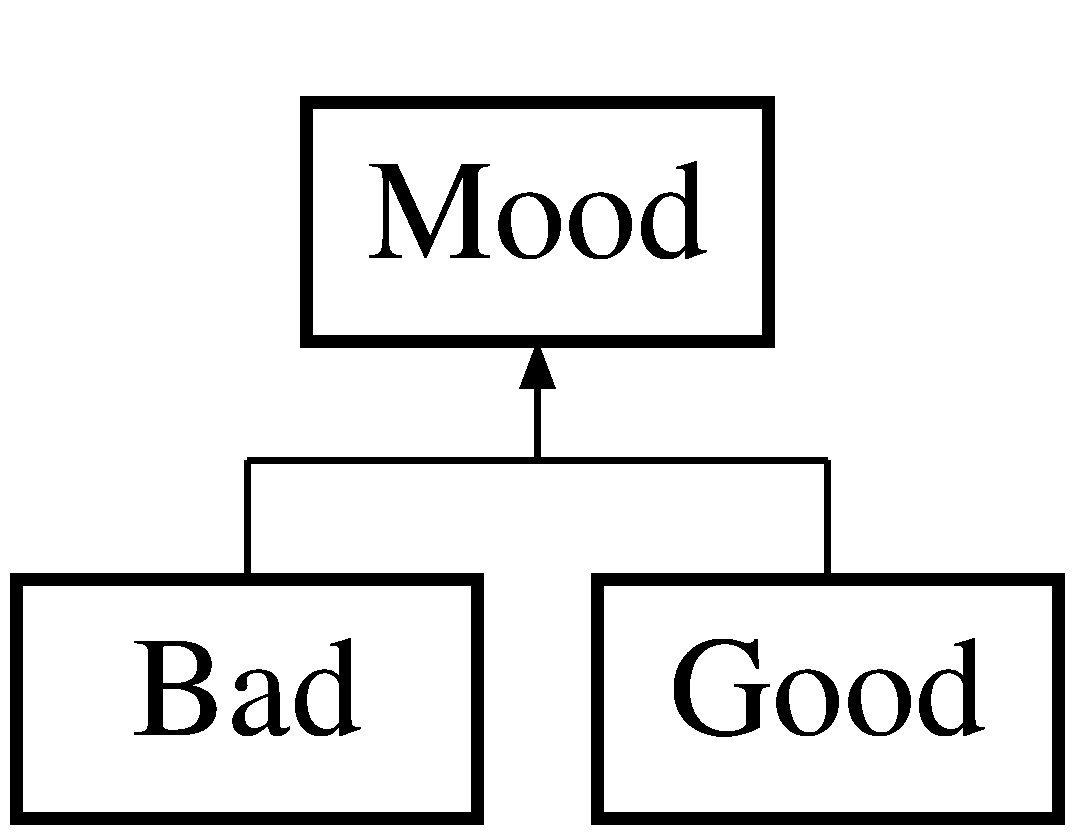
\includegraphics[height=2.000000cm]{class_mood}
\end{center}
\end{figure}


\subsection{Detailed Description}
\hyperlink{class_mood}{Mood}. 

\begin{DoxyAuthor}{Author}
Hamish Carrier 
\end{DoxyAuthor}
\begin{DoxyDate}{Date}
10/11/2013 
\end{DoxyDate}


The documentation for this class was generated from the following file\-:\begin{DoxyCompactItemize}
\item 
A\-:/\-I\-T/\-Git\-Hub/\-I\-C\-T312/source/ogregraphics/\hyperlink{_mood_8h}{Mood.\-h}\end{DoxyCompactItemize}

\hypertarget{class_mood_manager}{\section{Mood\-Manager Class Reference}
\label{class_mood_manager}\index{Mood\-Manager@{Mood\-Manager}}
}


Manager for moods.  




{\ttfamily \#include $<$Mood\-Manager.\-h$>$}

\subsection*{Public Member Functions}
\begin{DoxyCompactItemize}
\item 
\hyperlink{class_mood}{Mood} $\ast$ \hyperlink{class_mood_manager_a6124f65e1bd75b7025f1475e4e9a6577}{Fetch\-Mood} (Enum\-Space\-::\-Mood\-Types Desired\-Mood)
\begin{DoxyCompactList}\small\item\em Fetches a mood. \end{DoxyCompactList}\item 
void \hyperlink{class_mood_manager_a76b0af2237a77cc73a108ccd283de0ae}{Initialise\-Mood} (Enum\-Space\-::\-Mood\-Types Mood\-Type, int $\ast$Multipliers)
\begin{DoxyCompactList}\small\item\em Initialises the mood. \end{DoxyCompactList}\item 
std\-::map\\*
$<$ Enum\-Space\-::\-Emotion\-Types, int $>$ \hyperlink{class_mood_manager_a6e5c7fd531f190049e5c2be208f62dce}{Get\-Emotion\-Multipliers} (Enum\-Space\-::\-Mood\-Types Mood\-Type)
\begin{DoxyCompactList}\small\item\em Gets emotion multipliers. \end{DoxyCompactList}\item 
void \hyperlink{class_mood_manager_a401c3008ed0fe50c3766963ced3c5a21}{Init} (void)
\begin{DoxyCompactList}\small\item\em Initialises this object. \end{DoxyCompactList}\end{DoxyCompactItemize}
\subsection*{Static Public Member Functions}
\begin{DoxyCompactItemize}
\item 
static \hyperlink{class_mood_manager}{Mood\-Manager} $\ast$ \hyperlink{class_mood_manager_a66be018d05402aaeb081411cbe6fc27b}{Get\-Instance} ()
\begin{DoxyCompactList}\small\item\em Gets the instance. \end{DoxyCompactList}\end{DoxyCompactItemize}


\subsection{Detailed Description}
Manager for moods. 

\begin{DoxyAuthor}{Author}
Hamish Carrier 
\end{DoxyAuthor}
\begin{DoxyDate}{Date}
10/11/2013 
\end{DoxyDate}


\subsection{Member Function Documentation}
\hypertarget{class_mood_manager_a6124f65e1bd75b7025f1475e4e9a6577}{\index{Mood\-Manager@{Mood\-Manager}!Fetch\-Mood@{Fetch\-Mood}}
\index{Fetch\-Mood@{Fetch\-Mood}!MoodManager@{Mood\-Manager}}
\subsubsection[{Fetch\-Mood}]{\setlength{\rightskip}{0pt plus 5cm}{\bf Mood} $\ast$ Mood\-Manager\-::\-Fetch\-Mood (
\begin{DoxyParamCaption}
\item[{Enum\-Space\-::\-Mood\-Types}]{Desired\-Mood}
\end{DoxyParamCaption}
)}}\label{class_mood_manager_a6124f65e1bd75b7025f1475e4e9a6577}


Fetches a mood. 

\begin{DoxyAuthor}{Author}
Hamish Carrier 
\end{DoxyAuthor}
\begin{DoxyDate}{Date}
10/11/2013
\end{DoxyDate}

\begin{DoxyParams}{Parameters}
{\em Desired\-Mood} & The desired mood.\\
\hline
\end{DoxyParams}
\begin{DoxyReturn}{Returns}
null if it fails, else the mood. 
\end{DoxyReturn}
\hypertarget{class_mood_manager_a6e5c7fd531f190049e5c2be208f62dce}{\index{Mood\-Manager@{Mood\-Manager}!Get\-Emotion\-Multipliers@{Get\-Emotion\-Multipliers}}
\index{Get\-Emotion\-Multipliers@{Get\-Emotion\-Multipliers}!MoodManager@{Mood\-Manager}}
\subsubsection[{Get\-Emotion\-Multipliers}]{\setlength{\rightskip}{0pt plus 5cm}std\-::map$<$ Enum\-Space\-::\-Emotion\-Types, int $>$ Mood\-Manager\-::\-Get\-Emotion\-Multipliers (
\begin{DoxyParamCaption}
\item[{Enum\-Space\-::\-Mood\-Types}]{Mood\-Type}
\end{DoxyParamCaption}
)}}\label{class_mood_manager_a6e5c7fd531f190049e5c2be208f62dce}


Gets emotion multipliers. 

\begin{DoxyAuthor}{Author}
Hamish Carrier 
\end{DoxyAuthor}
\begin{DoxyDate}{Date}
10/11/2013
\end{DoxyDate}

\begin{DoxyParams}{Parameters}
{\em Mood\-Type} & Type of the mood.\\
\hline
\end{DoxyParams}
\begin{DoxyReturn}{Returns}
The emotion multipliers. 
\end{DoxyReturn}
\hypertarget{class_mood_manager_a66be018d05402aaeb081411cbe6fc27b}{\index{Mood\-Manager@{Mood\-Manager}!Get\-Instance@{Get\-Instance}}
\index{Get\-Instance@{Get\-Instance}!MoodManager@{Mood\-Manager}}
\subsubsection[{Get\-Instance}]{\setlength{\rightskip}{0pt plus 5cm}static {\bf Mood\-Manager} $\ast$ Mood\-Manager\-::\-Get\-Instance (
\begin{DoxyParamCaption}
{}
\end{DoxyParamCaption}
)\hspace{0.3cm}{\ttfamily [static]}}}\label{class_mood_manager_a66be018d05402aaeb081411cbe6fc27b}


Gets the instance. 

\begin{DoxyAuthor}{Author}
Hamish Carrier 
\end{DoxyAuthor}
\begin{DoxyDate}{Date}
10/11/2013
\end{DoxyDate}
\begin{DoxyReturn}{Returns}
null if it fails, else the instance. 
\end{DoxyReturn}
\hypertarget{class_mood_manager_a401c3008ed0fe50c3766963ced3c5a21}{\index{Mood\-Manager@{Mood\-Manager}!Init@{Init}}
\index{Init@{Init}!MoodManager@{Mood\-Manager}}
\subsubsection[{Init}]{\setlength{\rightskip}{0pt plus 5cm}void Mood\-Manager\-::\-Init (
\begin{DoxyParamCaption}
\item[{void}]{}
\end{DoxyParamCaption}
)}}\label{class_mood_manager_a401c3008ed0fe50c3766963ced3c5a21}


Initialises this object. 

\begin{DoxyAuthor}{Author}
Hamish Carrier 
\end{DoxyAuthor}
\begin{DoxyDate}{Date}
10/11/2013 
\end{DoxyDate}
\hypertarget{class_mood_manager_a76b0af2237a77cc73a108ccd283de0ae}{\index{Mood\-Manager@{Mood\-Manager}!Initialise\-Mood@{Initialise\-Mood}}
\index{Initialise\-Mood@{Initialise\-Mood}!MoodManager@{Mood\-Manager}}
\subsubsection[{Initialise\-Mood}]{\setlength{\rightskip}{0pt plus 5cm}void Mood\-Manager\-::\-Initialise\-Mood (
\begin{DoxyParamCaption}
\item[{Enum\-Space\-::\-Mood\-Types}]{Mood\-Type, }
\item[{int $\ast$}]{Multipliers}
\end{DoxyParamCaption}
)}}\label{class_mood_manager_a76b0af2237a77cc73a108ccd283de0ae}


Initialises the mood. 

\begin{DoxyAuthor}{Author}
Hamish Carrier 
\end{DoxyAuthor}
\begin{DoxyDate}{Date}
10/11/2013
\end{DoxyDate}

\begin{DoxyParams}[1]{Parameters}
 & {\em Mood\-Type} & Type of the mood. \\
\hline
\mbox{\tt in,out}  & {\em Multipliers} & If non-\/null, the multipliers. \\
\hline
\end{DoxyParams}


The documentation for this class was generated from the following files\-:\begin{DoxyCompactItemize}
\item 
A\-:/\-I\-T/\-Git\-Hub/\-I\-C\-T312/source/ogregraphics/\hyperlink{_mood_manager_8h}{Mood\-Manager.\-h}\item 
A\-:/\-I\-T/\-Git\-Hub/\-I\-C\-T312/source/ogregraphics/Mood\-Manager.\-cpp\end{DoxyCompactItemize}

\hypertarget{class_move_item}{\section{Move\-Item Class Reference}
\label{class_move_item}\index{Move\-Item@{Move\-Item}}
}


Move item.  




{\ttfamily \#include $<$Move\-Item.\-h$>$}

Inheritance diagram for Move\-Item\-:\begin{figure}[H]
\begin{center}
\leavevmode
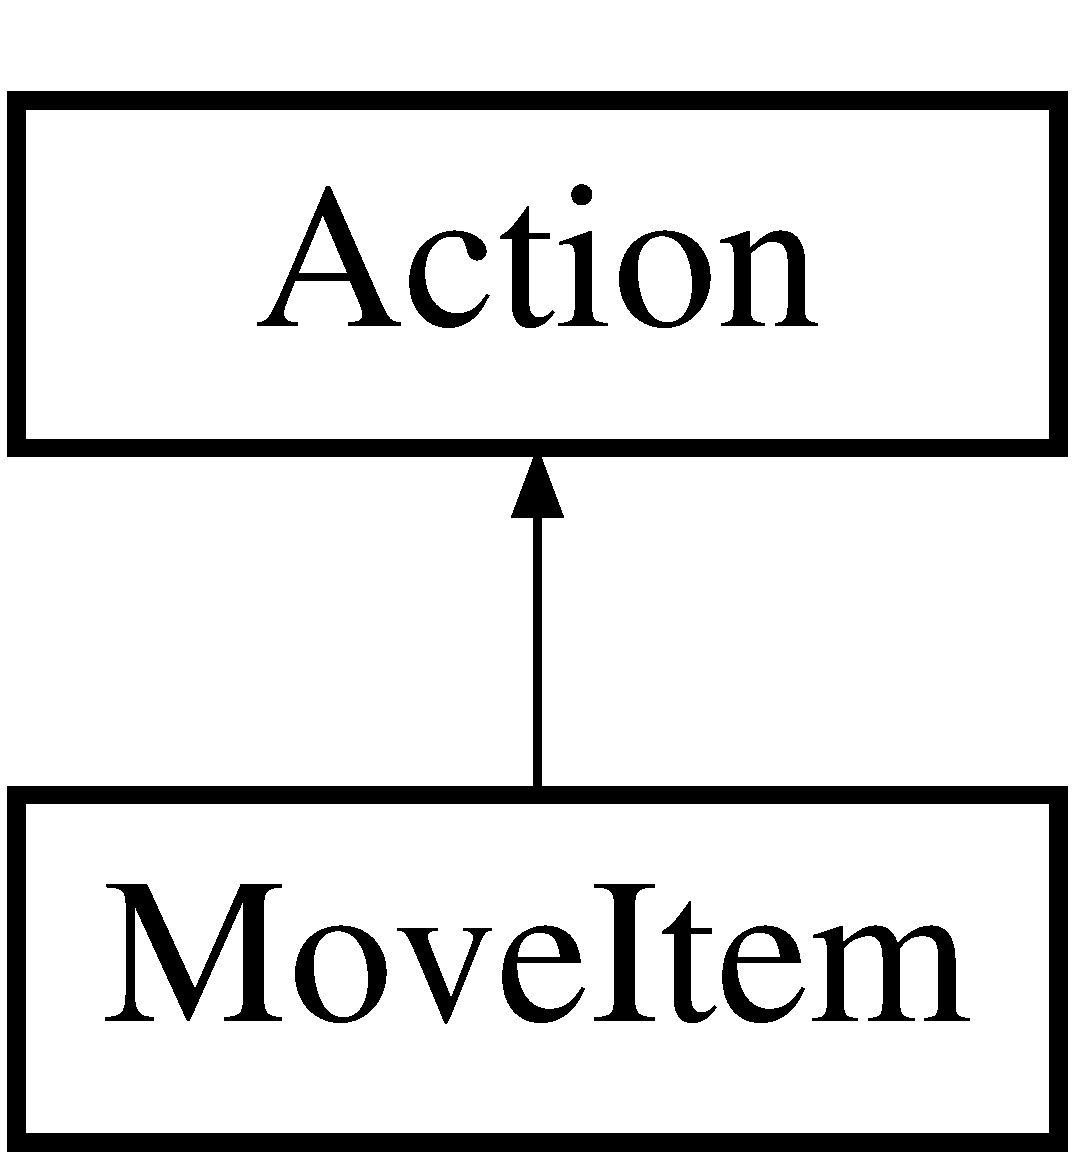
\includegraphics[height=2.000000cm]{class_move_item}
\end{center}
\end{figure}
\subsection*{Public Member Functions}
\begin{DoxyCompactItemize}
\item 
\hyperlink{class_move_item_a7e55e7661437d954afaa1a8359c04df1}{Move\-Item} (void)
\begin{DoxyCompactList}\small\item\em Default constructor. \end{DoxyCompactList}\item 
\hyperlink{class_move_item_a4a74c891971cb30e216a8811db9f9a84}{$\sim$\-Move\-Item} (void)
\begin{DoxyCompactList}\small\item\em Destructor. \end{DoxyCompactList}\end{DoxyCompactItemize}


\subsection{Detailed Description}
Move item. 

\begin{DoxyAuthor}{Author}
Hamish Carrier 
\end{DoxyAuthor}
\begin{DoxyDate}{Date}
10/11/2013 
\end{DoxyDate}


\subsection{Constructor \& Destructor Documentation}
\hypertarget{class_move_item_a7e55e7661437d954afaa1a8359c04df1}{\index{Move\-Item@{Move\-Item}!Move\-Item@{Move\-Item}}
\index{Move\-Item@{Move\-Item}!MoveItem@{Move\-Item}}
\subsubsection[{Move\-Item}]{\setlength{\rightskip}{0pt plus 5cm}Move\-Item\-::\-Move\-Item (
\begin{DoxyParamCaption}
\item[{void}]{}
\end{DoxyParamCaption}
)}}\label{class_move_item_a7e55e7661437d954afaa1a8359c04df1}


Default constructor. 

\begin{DoxyAuthor}{Author}
Hamish Carrier 
\end{DoxyAuthor}
\begin{DoxyDate}{Date}
10/11/2013 
\end{DoxyDate}
\hypertarget{class_move_item_a4a74c891971cb30e216a8811db9f9a84}{\index{Move\-Item@{Move\-Item}!$\sim$\-Move\-Item@{$\sim$\-Move\-Item}}
\index{$\sim$\-Move\-Item@{$\sim$\-Move\-Item}!MoveItem@{Move\-Item}}
\subsubsection[{$\sim$\-Move\-Item}]{\setlength{\rightskip}{0pt plus 5cm}Move\-Item\-::$\sim$\-Move\-Item (
\begin{DoxyParamCaption}
\item[{void}]{}
\end{DoxyParamCaption}
)}}\label{class_move_item_a4a74c891971cb30e216a8811db9f9a84}


Destructor. 

\begin{DoxyAuthor}{Author}
Hamish Carrier 
\end{DoxyAuthor}
\begin{DoxyDate}{Date}
10/11/2013 
\end{DoxyDate}


The documentation for this class was generated from the following files\-:\begin{DoxyCompactItemize}
\item 
A\-:/\-I\-T/\-Git\-Hub/\-I\-C\-T312/source/ogregraphics/\hyperlink{_move_item_8h}{Move\-Item.\-h}\item 
A\-:/\-I\-T/\-Git\-Hub/\-I\-C\-T312/source/ogregraphics/Move\-Item.\-cpp\end{DoxyCompactItemize}

\hypertarget{class_my_convex_decomposition}{\section{My\-Convex\-Decomposition Class Reference}
\label{class_my_convex_decomposition}\index{My\-Convex\-Decomposition@{My\-Convex\-Decomposition}}
}
Inheritance diagram for My\-Convex\-Decomposition\-:\begin{figure}[H]
\begin{center}
\leavevmode
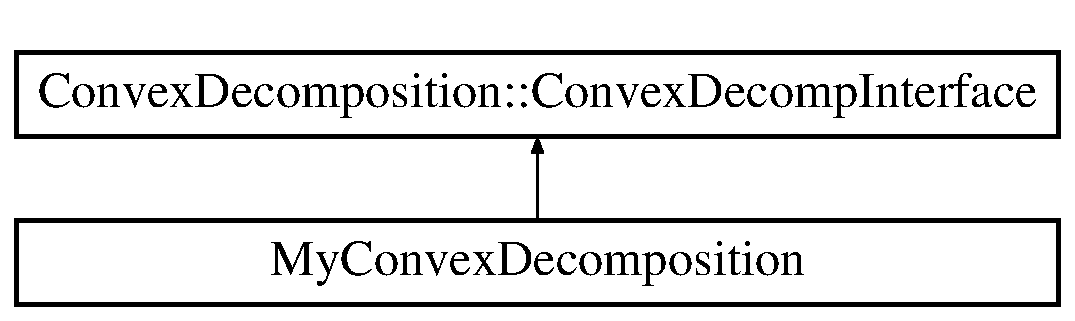
\includegraphics[height=2.000000cm]{class_my_convex_decomposition}
\end{center}
\end{figure}
\subsection*{Public Member Functions}
\begin{DoxyCompactItemize}
\item 
\hypertarget{class_my_convex_decomposition_a3abbe41135a655ce5be0fc8162dd742b}{virtual void {\bfseries Convex\-Decomp\-Result} (\hyperlink{class_convex_decomposition_1_1_convex_result}{Convex\-Decomposition\-::\-Convex\-Result} \&result)}\label{class_my_convex_decomposition_a3abbe41135a655ce5be0fc8162dd742b}

\end{DoxyCompactItemize}
\subsection*{Public Attributes}
\begin{DoxyCompactItemize}
\item 
\hypertarget{class_my_convex_decomposition_a6c7e2375dbc914f33750f9c59b3cd599}{bt\-Aligned\-Object\-Array\\*
$<$ bt\-Convex\-Hull\-Shape $\ast$ $>$ {\bfseries m\-\_\-convex\-Shapes}}\label{class_my_convex_decomposition_a6c7e2375dbc914f33750f9c59b3cd599}

\item 
\hypertarget{class_my_convex_decomposition_abb3bf59567cac3c5ddc948b0fecb04ae}{bt\-Aligned\-Object\-Array$<$ bt\-Vector3 $>$ {\bfseries m\-\_\-convex\-Centroids}}\label{class_my_convex_decomposition_abb3bf59567cac3c5ddc948b0fecb04ae}

\item 
\hypertarget{class_my_convex_decomposition_a387f1cbfa3161db25dbaeaf60cf1e6dd}{int {\bfseries m\-Base\-Count}}\label{class_my_convex_decomposition_a387f1cbfa3161db25dbaeaf60cf1e6dd}

\item 
\hypertarget{class_my_convex_decomposition_a1e14fdd3dc8255dc5d77fb0a17f528e5}{int {\bfseries m\-Hull\-Count}}\label{class_my_convex_decomposition_a1e14fdd3dc8255dc5d77fb0a17f528e5}

\item 
\hypertarget{class_my_convex_decomposition_a39a3749d2d7c5643aec6ee178fd65fdb}{bt\-Vector3 {\bfseries m\-Centroid}}\label{class_my_convex_decomposition_a39a3749d2d7c5643aec6ee178fd65fdb}

\item 
\hypertarget{class_my_convex_decomposition_a22783181be65e4e9c9a94f74cfb6a012}{bt\-Vector3 {\bfseries convex\-Decomposition\-Object\-Offset}}\label{class_my_convex_decomposition_a22783181be65e4e9c9a94f74cfb6a012}

\end{DoxyCompactItemize}


The documentation for this class was generated from the following file\-:\begin{DoxyCompactItemize}
\item 
A\-:/\-I\-T/\-Git\-Hub/\-I\-C\-T312/source/ogregraphics/Ogre\-Bullet\-Collisions\-Mesh\-To\-Shape\-Converter.\-cpp\end{DoxyCompactItemize}

\hypertarget{class_neutral}{\section{Neutral Class Reference}
\label{class_neutral}\index{Neutral@{Neutral}}
}


\hyperlink{class_neutral}{Neutral}.  




{\ttfamily \#include $<$Neutral.\-h$>$}

Inheritance diagram for Neutral\-:\begin{figure}[H]
\begin{center}
\leavevmode
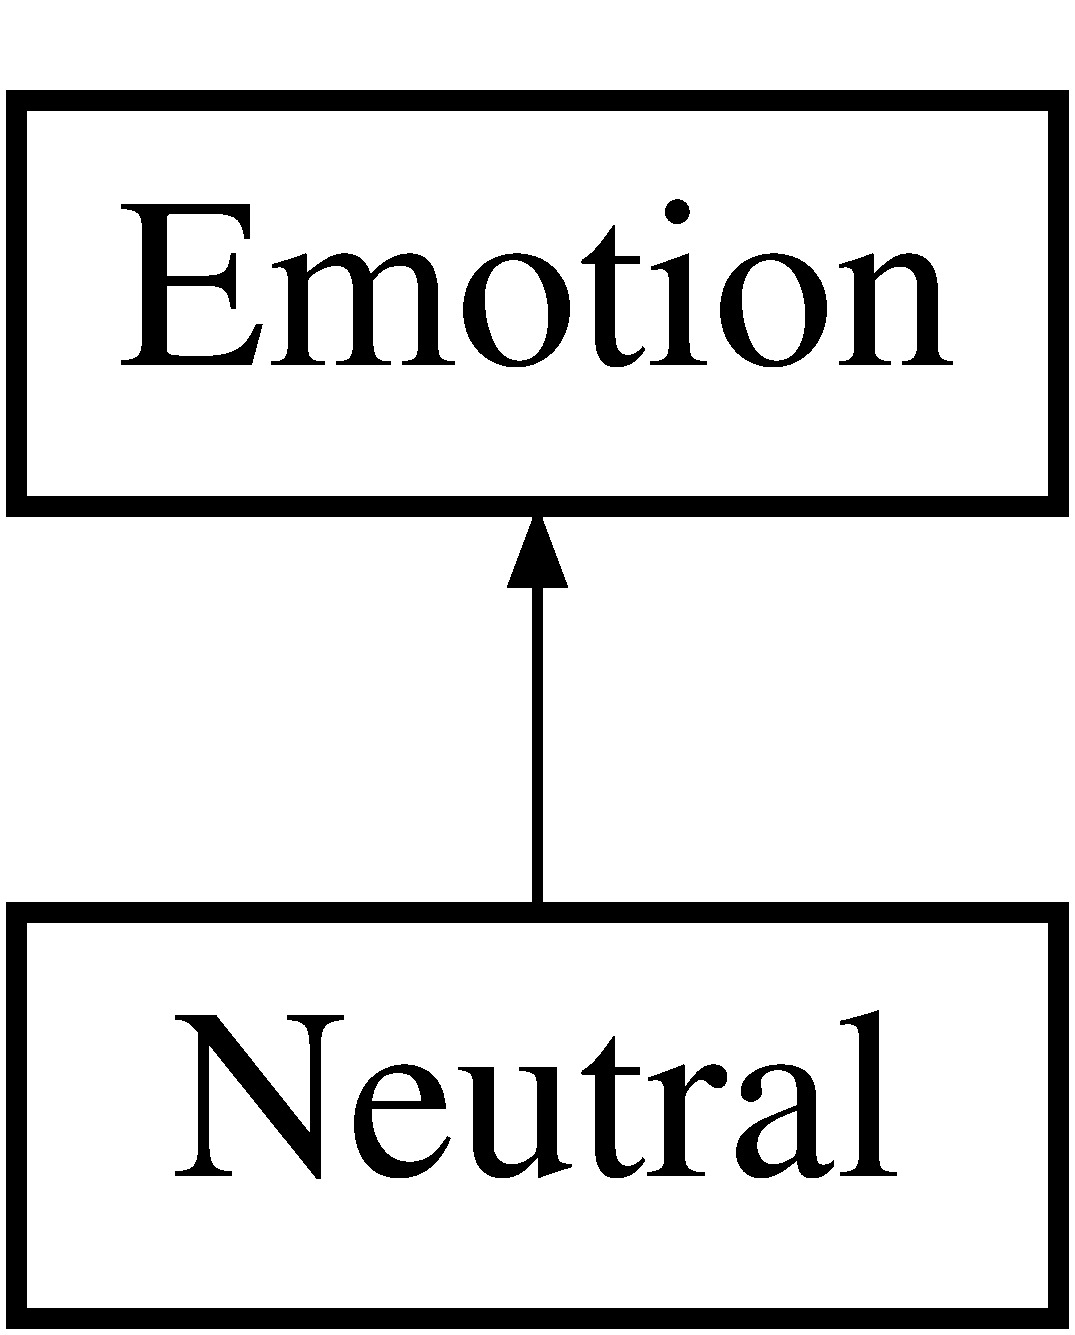
\includegraphics[height=2.000000cm]{class_neutral}
\end{center}
\end{figure}
\subsection*{Public Member Functions}
\begin{DoxyCompactItemize}
\item 
\hyperlink{class_neutral_a95ea8b98ebc51b5f7b3cc2bf3f1b0c84}{Neutral} (void)
\begin{DoxyCompactList}\small\item\em Default constructor. \end{DoxyCompactList}\item 
\hyperlink{class_neutral_aeb83d32f088f64c60a4aca15a0631d0f}{$\sim$\-Neutral} (void)
\begin{DoxyCompactList}\small\item\em Destructor. \end{DoxyCompactList}\end{DoxyCompactItemize}


\subsection{Detailed Description}
\hyperlink{class_neutral}{Neutral}. 

\begin{DoxyAuthor}{Author}
Hamish Carrier 
\end{DoxyAuthor}
\begin{DoxyDate}{Date}
10/11/2013 
\end{DoxyDate}


\subsection{Constructor \& Destructor Documentation}
\hypertarget{class_neutral_a95ea8b98ebc51b5f7b3cc2bf3f1b0c84}{\index{Neutral@{Neutral}!Neutral@{Neutral}}
\index{Neutral@{Neutral}!Neutral@{Neutral}}
\subsubsection[{Neutral}]{\setlength{\rightskip}{0pt plus 5cm}Neutral\-::\-Neutral (
\begin{DoxyParamCaption}
\item[{void}]{}
\end{DoxyParamCaption}
)}}\label{class_neutral_a95ea8b98ebc51b5f7b3cc2bf3f1b0c84}


Default constructor. 

\begin{DoxyAuthor}{Author}
Hamish Carrier 
\end{DoxyAuthor}
\begin{DoxyDate}{Date}
10/11/2013 
\end{DoxyDate}
\hypertarget{class_neutral_aeb83d32f088f64c60a4aca15a0631d0f}{\index{Neutral@{Neutral}!$\sim$\-Neutral@{$\sim$\-Neutral}}
\index{$\sim$\-Neutral@{$\sim$\-Neutral}!Neutral@{Neutral}}
\subsubsection[{$\sim$\-Neutral}]{\setlength{\rightskip}{0pt plus 5cm}Neutral\-::$\sim$\-Neutral (
\begin{DoxyParamCaption}
\item[{void}]{}
\end{DoxyParamCaption}
)}}\label{class_neutral_aeb83d32f088f64c60a4aca15a0631d0f}


Destructor. 

\begin{DoxyAuthor}{Author}
Hamish Carrier 
\end{DoxyAuthor}
\begin{DoxyDate}{Date}
10/11/2013 
\end{DoxyDate}


The documentation for this class was generated from the following files\-:\begin{DoxyCompactItemize}
\item 
A\-:/\-I\-T/\-Git\-Hub/\-I\-C\-T312/source/ogregraphics/\hyperlink{_neutral_8h}{Neutral.\-h}\item 
A\-:/\-I\-T/\-Git\-Hub/\-I\-C\-T312/source/ogregraphics/Neutral.\-cpp\end{DoxyCompactItemize}

\hypertarget{class_node_container_singleton}{\section{Node\-Container\-Singleton Class Reference}
\label{class_node_container_singleton}\index{Node\-Container\-Singleton@{Node\-Container\-Singleton}}
}


Node container singleton this is the class that contains all the nodes that make up the world for pathing.  




{\ttfamily \#include $<$Node\-Container\-Singleton.\-h$>$}

\subsection*{Public Member Functions}
\begin{DoxyCompactItemize}
\item 
\hyperlink{class_map_node}{Map\-Node} $\ast$ \hyperlink{class_node_container_singleton_a8dc436b2278212ffe2063438f54cd6a9}{Find\-Nearest\-Node} (Ogre\-::\-Vector3 Position)
\begin{DoxyCompactList}\small\item\em Searches for the nearest node to a postion. \end{DoxyCompactList}\end{DoxyCompactItemize}
\subsection*{Static Public Member Functions}
\begin{DoxyCompactItemize}
\item 
static \hyperlink{class_node_container_singleton}{Node\-Container\-Singleton} $\ast$ \hyperlink{class_node_container_singleton_ad9e8f40bc5677d244037299cfc29a7b9}{Instance} ()
\begin{DoxyCompactList}\small\item\em Gets the instance. \end{DoxyCompactList}\end{DoxyCompactItemize}


\subsection{Detailed Description}
Node container singleton this is the class that contains all the nodes that make up the world for pathing. 

\begin{DoxyAuthor}{Author}
Arran Ford 
\end{DoxyAuthor}
\begin{DoxyDate}{Date}
09/11/2013 
\end{DoxyDate}


\subsection{Member Function Documentation}
\hypertarget{class_node_container_singleton_a8dc436b2278212ffe2063438f54cd6a9}{\index{Node\-Container\-Singleton@{Node\-Container\-Singleton}!Find\-Nearest\-Node@{Find\-Nearest\-Node}}
\index{Find\-Nearest\-Node@{Find\-Nearest\-Node}!NodeContainerSingleton@{Node\-Container\-Singleton}}
\subsubsection[{Find\-Nearest\-Node}]{\setlength{\rightskip}{0pt plus 5cm}{\bf Map\-Node} $\ast$ Node\-Container\-Singleton\-::\-Find\-Nearest\-Node (
\begin{DoxyParamCaption}
\item[{Ogre\-::\-Vector3}]{Position}
\end{DoxyParamCaption}
)}}\label{class_node_container_singleton_a8dc436b2278212ffe2063438f54cd6a9}


Searches for the nearest node to a postion. 

\begin{DoxyAuthor}{Author}
Arran Ford 
\end{DoxyAuthor}
\begin{DoxyDate}{Date}
09/11/2013
\end{DoxyDate}

\begin{DoxyParams}{Parameters}
{\em Position} & The position.\\
\hline
\end{DoxyParams}
\begin{DoxyReturn}{Returns}
null if it fails, else the found node. 
\end{DoxyReturn}
\hypertarget{class_node_container_singleton_ad9e8f40bc5677d244037299cfc29a7b9}{\index{Node\-Container\-Singleton@{Node\-Container\-Singleton}!Instance@{Instance}}
\index{Instance@{Instance}!NodeContainerSingleton@{Node\-Container\-Singleton}}
\subsubsection[{Instance}]{\setlength{\rightskip}{0pt plus 5cm}static {\bf Node\-Container\-Singleton} $\ast$ Node\-Container\-Singleton\-::\-Instance (
\begin{DoxyParamCaption}
{}
\end{DoxyParamCaption}
)\hspace{0.3cm}{\ttfamily [static]}}}\label{class_node_container_singleton_ad9e8f40bc5677d244037299cfc29a7b9}


Gets the instance. 

\begin{DoxyAuthor}{Author}
Arran Ford 
\end{DoxyAuthor}
\begin{DoxyDate}{Date}
09/11/2013
\end{DoxyDate}
\begin{DoxyReturn}{Returns}
null if it fails, else. 
\end{DoxyReturn}


The documentation for this class was generated from the following files\-:\begin{DoxyCompactItemize}
\item 
A\-:/\-I\-T/\-Git\-Hub/\-I\-C\-T312/source/ogregraphics/\hyperlink{_node_container_singleton_8h}{Node\-Container\-Singleton.\-h}\item 
A\-:/\-I\-T/\-Git\-Hub/\-I\-C\-T312/source/ogregraphics/Node\-Container\-Singleton.\-cpp\end{DoxyCompactItemize}

\hypertarget{structmicropather_1_1_node_cost}{\section{micropather\-:\-:Node\-Cost Struct Reference}
\label{structmicropather_1_1_node_cost}\index{micropather\-::\-Node\-Cost@{micropather\-::\-Node\-Cost}}
}
\subsection*{Public Attributes}
\begin{DoxyCompactItemize}
\item 
\hypertarget{structmicropather_1_1_node_cost_a0fac510eb20aeaa8704363b4af5177f8}{\hyperlink{classmicropather_1_1_path_node}{Path\-Node} $\ast$ {\bfseries node}}\label{structmicropather_1_1_node_cost_a0fac510eb20aeaa8704363b4af5177f8}

\item 
\hypertarget{structmicropather_1_1_node_cost_a633396145abc66f6bc93830c2f76ca23}{float {\bfseries cost}}\label{structmicropather_1_1_node_cost_a633396145abc66f6bc93830c2f76ca23}

\end{DoxyCompactItemize}


The documentation for this struct was generated from the following file\-:\begin{DoxyCompactItemize}
\item 
A\-:/\-I\-T/\-Git\-Hub/\-I\-C\-T312/source/ogregraphics/micropather.\-h\end{DoxyCompactItemize}

\hypertarget{class_n_p_c}{\section{N\-P\-C Class Reference}
\label{class_n_p_c}\index{N\-P\-C@{N\-P\-C}}
}


Npc.  




{\ttfamily \#include $<$N\-P\-C.\-h$>$}

\subsection*{Public Member Functions}
\begin{DoxyCompactItemize}
\item 
\hyperlink{class_n_p_c_af28ce051772f77e3b3c95545067d5ef5}{N\-P\-C} (void)
\begin{DoxyCompactList}\small\item\em Default constructor. \end{DoxyCompactList}\item 
\hyperlink{class_n_p_c_ad96ce7664caaec2d176bf64cac1c4df8}{N\-P\-C} (\hyperlink{class_objects_1_1_i_object}{Objects\-::\-I\-Object} $\ast$Obj)
\begin{DoxyCompactList}\small\item\em Constructor. \end{DoxyCompactList}\item 
\hyperlink{class_n_p_c_a82bd4ced6842c4ed6638e414c2b75640}{$\sim$\-N\-P\-C} (void)
\begin{DoxyCompactList}\small\item\em Destructor. \end{DoxyCompactList}\item 
bool \hyperlink{class_n_p_c_a5bd9cfaa9afa94bf3255c0ab0a6ccf1f}{Emotion\-Check} ()
\begin{DoxyCompactList}\small\item\em Determines if we can emotion check. \end{DoxyCompactList}\item 
bool \hyperlink{class_n_p_c_a40494bd49dfc0a28a71869afee79993b}{Determine\-Goal} ()
\begin{DoxyCompactList}\small\item\em Determines if we can determine goal. \end{DoxyCompactList}\item 
void \hyperlink{class_n_p_c_a30bba3999124a895a553cb93a0f094e2}{Check\-Goal} ()
\begin{DoxyCompactList}\small\item\em Check goal. \end{DoxyCompactList}\item 
void \hyperlink{class_n_p_c_af62e98d4bc6e38d355934fe41511d2b4}{Update} ()
\begin{DoxyCompactList}\small\item\em Updates this object. \end{DoxyCompactList}\item 
void \hyperlink{class_n_p_c_a19ffac02c2add2ac1a4a77a0f73bbd2f}{Initialise} ()
\begin{DoxyCompactList}\small\item\em Initialises this object. \end{DoxyCompactList}\item 
bool \hyperlink{class_n_p_c_abc15c4dbd9dea30968cbf01e4e723f65}{run\-Current\-State} ()
\begin{DoxyCompactList}\small\item\em Executes the current state operation. \end{DoxyCompactList}\item 
void \hyperlink{class_n_p_c_afdc85c2f160a4d2ce51afb33385fe425}{Progress\-Mood} (Enum\-Space\-::\-Emotion\-Types S)
\begin{DoxyCompactList}\small\item\em Progress mood. \end{DoxyCompactList}\item 
void \hyperlink{class_n_p_c_ab9c846d51a96ad4eb0cb676bfc35d9bb}{Clicked} (std\-::string click)
\begin{DoxyCompactList}\small\item\em Clickeds the given click. \end{DoxyCompactList}\end{DoxyCompactItemize}
\subsection*{Protected Attributes}
\begin{DoxyCompactItemize}
\item 
\hypertarget{class_n_p_c_a70f1d72ce96cfe4800a4bb7ce4cb4a8c}{\hyperlink{class_action}{Action} $\ast$ \hyperlink{class_n_p_c_a70f1d72ce96cfe4800a4bb7ce4cb4a8c}{Current\-Action}}\label{class_n_p_c_a70f1d72ce96cfe4800a4bb7ce4cb4a8c}

\begin{DoxyCompactList}\small\item\em The current action. \end{DoxyCompactList}\item 
\hypertarget{class_n_p_c_aacdb21f730d86fb68b70f88bf4a1eefe}{\hyperlink{class_emotion}{Emotion} $\ast$ \hyperlink{class_n_p_c_aacdb21f730d86fb68b70f88bf4a1eefe}{Current\-Emotion}}\label{class_n_p_c_aacdb21f730d86fb68b70f88bf4a1eefe}

\begin{DoxyCompactList}\small\item\em The current emotion. \end{DoxyCompactList}\item 
\hypertarget{class_n_p_c_a46cedade10fa9f48531a52d5d1913b1b}{\hyperlink{class_mood}{Mood} $\ast$ \hyperlink{class_n_p_c_a46cedade10fa9f48531a52d5d1913b1b}{Current\-Mood}}\label{class_n_p_c_a46cedade10fa9f48531a52d5d1913b1b}

\begin{DoxyCompactList}\small\item\em The current mood. \end{DoxyCompactList}\item 
\hypertarget{class_n_p_c_a44a39ba5690ce740a814b8f925c74165}{\hyperlink{class_goal}{Goal} $\ast$ \hyperlink{class_n_p_c_a44a39ba5690ce740a814b8f925c74165}{Current\-Goal}}\label{class_n_p_c_a44a39ba5690ce740a814b8f925c74165}

\begin{DoxyCompactList}\small\item\em The current goal. \end{DoxyCompactList}\item 
\hypertarget{class_n_p_c_a3593aab52251644d5aa4996452fc5d27}{Enum\-Space\-::\-N\-P\-C\-State \hyperlink{class_n_p_c_a3593aab52251644d5aa4996452fc5d27}{Current\-State}}\label{class_n_p_c_a3593aab52251644d5aa4996452fc5d27}

\begin{DoxyCompactList}\small\item\em The current state. \end{DoxyCompactList}\item 
\hypertarget{class_n_p_c_a4425a1bed44cba46cbfb4c5242b3781f}{\hyperlink{class_trait}{Trait} $\ast$ \hyperlink{class_n_p_c_a4425a1bed44cba46cbfb4c5242b3781f}{my\-Trait}}\label{class_n_p_c_a4425a1bed44cba46cbfb4c5242b3781f}

\begin{DoxyCompactList}\small\item\em my trait. \end{DoxyCompactList}\item 
\hypertarget{class_n_p_c_af73bcc764619d81248b70441f26d3c52}{\hyperlink{class_objects_1_1_i_object}{Objects\-::\-I\-Object} $\ast$ \hyperlink{class_n_p_c_af73bcc764619d81248b70441f26d3c52}{my\-Obj}}\label{class_n_p_c_af73bcc764619d81248b70441f26d3c52}

\begin{DoxyCompactList}\small\item\em my object. \end{DoxyCompactList}\item 
\hypertarget{class_n_p_c_a562d859408ecbdcbb17f6d7fd8d59aa1}{\hyperlink{class_objects_1_1_i_object}{Objects\-::\-I\-Object} $\ast$ \hyperlink{class_n_p_c_a562d859408ecbdcbb17f6d7fd8d59aa1}{Object\-Pointer}}\label{class_n_p_c_a562d859408ecbdcbb17f6d7fd8d59aa1}

\begin{DoxyCompactList}\small\item\em The object pointer. \end{DoxyCompactList}\item 
std\-::map$<$ Enum\-Space\-::\-Need\-Types, \\*
int $>$ \hyperlink{class_n_p_c_a7521486609aac06982e95eebc0c57f6e}{Current\-Needs}
\begin{DoxyCompactList}\small\item\em Gets the current needs. \end{DoxyCompactList}\item 
\hypertarget{class_n_p_c_a5e6a93343caa98732e9c5ca4d5dc09f3}{std\-::map$<$ Enum\-Space\-::\-Mood\-Types, \\*
int $>$ \hyperlink{class_n_p_c_a5e6a93343caa98732e9c5ca4d5dc09f3}{Mood\-Progress}}\label{class_n_p_c_a5e6a93343caa98732e9c5ca4d5dc09f3}

\begin{DoxyCompactList}\small\item\em The mood progress. \end{DoxyCompactList}\end{DoxyCompactItemize}


\subsection{Detailed Description}
Npc. 

\begin{DoxyAuthor}{Author}
Hamish Carrier 
\end{DoxyAuthor}
\begin{DoxyDate}{Date}
10/11/2013 
\end{DoxyDate}


\subsection{Constructor \& Destructor Documentation}
\hypertarget{class_n_p_c_af28ce051772f77e3b3c95545067d5ef5}{\index{N\-P\-C@{N\-P\-C}!N\-P\-C@{N\-P\-C}}
\index{N\-P\-C@{N\-P\-C}!NPC@{N\-P\-C}}
\subsubsection[{N\-P\-C}]{\setlength{\rightskip}{0pt plus 5cm}N\-P\-C\-::\-N\-P\-C (
\begin{DoxyParamCaption}
\item[{void}]{}
\end{DoxyParamCaption}
)}}\label{class_n_p_c_af28ce051772f77e3b3c95545067d5ef5}


Default constructor. 

\begin{DoxyAuthor}{Author}
Hamish Carrier 
\end{DoxyAuthor}
\begin{DoxyDate}{Date}
10/11/2013 
\end{DoxyDate}
\hypertarget{class_n_p_c_ad96ce7664caaec2d176bf64cac1c4df8}{\index{N\-P\-C@{N\-P\-C}!N\-P\-C@{N\-P\-C}}
\index{N\-P\-C@{N\-P\-C}!NPC@{N\-P\-C}}
\subsubsection[{N\-P\-C}]{\setlength{\rightskip}{0pt plus 5cm}N\-P\-C\-::\-N\-P\-C (
\begin{DoxyParamCaption}
\item[{{\bf Objects\-::\-I\-Object} $\ast$}]{Obj}
\end{DoxyParamCaption}
)\hspace{0.3cm}{\ttfamily [inline]}}}\label{class_n_p_c_ad96ce7664caaec2d176bf64cac1c4df8}


Constructor. 

\begin{DoxyAuthor}{Author}
Hamish Carrier 
\end{DoxyAuthor}
\begin{DoxyDate}{Date}
10/11/2013
\end{DoxyDate}

\begin{DoxyParams}[1]{Parameters}
\mbox{\tt in,out}  & {\em Obj} & If non-\/null, the object. \\
\hline
\end{DoxyParams}
\hypertarget{class_n_p_c_a82bd4ced6842c4ed6638e414c2b75640}{\index{N\-P\-C@{N\-P\-C}!$\sim$\-N\-P\-C@{$\sim$\-N\-P\-C}}
\index{$\sim$\-N\-P\-C@{$\sim$\-N\-P\-C}!NPC@{N\-P\-C}}
\subsubsection[{$\sim$\-N\-P\-C}]{\setlength{\rightskip}{0pt plus 5cm}N\-P\-C\-::$\sim$\-N\-P\-C (
\begin{DoxyParamCaption}
\item[{void}]{}
\end{DoxyParamCaption}
)}}\label{class_n_p_c_a82bd4ced6842c4ed6638e414c2b75640}


Destructor. 

\begin{DoxyAuthor}{Author}
Hamish Carrier 
\end{DoxyAuthor}
\begin{DoxyDate}{Date}
10/11/2013 
\end{DoxyDate}


\subsection{Member Function Documentation}
\hypertarget{class_n_p_c_a30bba3999124a895a553cb93a0f094e2}{\index{N\-P\-C@{N\-P\-C}!Check\-Goal@{Check\-Goal}}
\index{Check\-Goal@{Check\-Goal}!NPC@{N\-P\-C}}
\subsubsection[{Check\-Goal}]{\setlength{\rightskip}{0pt plus 5cm}void N\-P\-C\-::\-Check\-Goal (
\begin{DoxyParamCaption}
{}
\end{DoxyParamCaption}
)}}\label{class_n_p_c_a30bba3999124a895a553cb93a0f094e2}


Check goal. 

\begin{DoxyAuthor}{Author}
Hamish Carrier 
\end{DoxyAuthor}
\begin{DoxyDate}{Date}
10/11/2013 
\end{DoxyDate}
\hypertarget{class_n_p_c_ab9c846d51a96ad4eb0cb676bfc35d9bb}{\index{N\-P\-C@{N\-P\-C}!Clicked@{Clicked}}
\index{Clicked@{Clicked}!NPC@{N\-P\-C}}
\subsubsection[{Clicked}]{\setlength{\rightskip}{0pt plus 5cm}void N\-P\-C\-::\-Clicked (
\begin{DoxyParamCaption}
\item[{std\-::string}]{click}
\end{DoxyParamCaption}
)}}\label{class_n_p_c_ab9c846d51a96ad4eb0cb676bfc35d9bb}


Clickeds the given click. 

\begin{DoxyAuthor}{Author}
Hamish Carrier 
\end{DoxyAuthor}
\begin{DoxyDate}{Date}
10/11/2013
\end{DoxyDate}

\begin{DoxyParams}{Parameters}
{\em click} & The click. \\
\hline
\end{DoxyParams}
\hypertarget{class_n_p_c_a40494bd49dfc0a28a71869afee79993b}{\index{N\-P\-C@{N\-P\-C}!Determine\-Goal@{Determine\-Goal}}
\index{Determine\-Goal@{Determine\-Goal}!NPC@{N\-P\-C}}
\subsubsection[{Determine\-Goal}]{\setlength{\rightskip}{0pt plus 5cm}bool N\-P\-C\-::\-Determine\-Goal (
\begin{DoxyParamCaption}
{}
\end{DoxyParamCaption}
)}}\label{class_n_p_c_a40494bd49dfc0a28a71869afee79993b}


Determines if we can determine goal. 

\begin{DoxyAuthor}{Author}
Hamish Carrier 
\end{DoxyAuthor}
\begin{DoxyDate}{Date}
10/11/2013
\end{DoxyDate}
\begin{DoxyReturn}{Returns}
true if it succeeds, false if it fails. 
\end{DoxyReturn}
\hypertarget{class_n_p_c_a5bd9cfaa9afa94bf3255c0ab0a6ccf1f}{\index{N\-P\-C@{N\-P\-C}!Emotion\-Check@{Emotion\-Check}}
\index{Emotion\-Check@{Emotion\-Check}!NPC@{N\-P\-C}}
\subsubsection[{Emotion\-Check}]{\setlength{\rightskip}{0pt plus 5cm}bool N\-P\-C\-::\-Emotion\-Check (
\begin{DoxyParamCaption}
\item[{void}]{}
\end{DoxyParamCaption}
)}}\label{class_n_p_c_a5bd9cfaa9afa94bf3255c0ab0a6ccf1f}


Determines if we can emotion check. 

\begin{DoxyAuthor}{Author}
Hamish Carrier 
\end{DoxyAuthor}
\begin{DoxyDate}{Date}
10/11/2013
\end{DoxyDate}
\begin{DoxyReturn}{Returns}
true if it succeeds, false if it fails. 
\end{DoxyReturn}
\hypertarget{class_n_p_c_a19ffac02c2add2ac1a4a77a0f73bbd2f}{\index{N\-P\-C@{N\-P\-C}!Initialise@{Initialise}}
\index{Initialise@{Initialise}!NPC@{N\-P\-C}}
\subsubsection[{Initialise}]{\setlength{\rightskip}{0pt plus 5cm}void N\-P\-C\-::\-Initialise (
\begin{DoxyParamCaption}
\item[{void}]{}
\end{DoxyParamCaption}
)}}\label{class_n_p_c_a19ffac02c2add2ac1a4a77a0f73bbd2f}


Initialises this object. 

\begin{DoxyAuthor}{Author}
Hamish Carrier 
\end{DoxyAuthor}
\begin{DoxyDate}{Date}
10/11/2013 
\end{DoxyDate}
\hypertarget{class_n_p_c_afdc85c2f160a4d2ce51afb33385fe425}{\index{N\-P\-C@{N\-P\-C}!Progress\-Mood@{Progress\-Mood}}
\index{Progress\-Mood@{Progress\-Mood}!NPC@{N\-P\-C}}
\subsubsection[{Progress\-Mood}]{\setlength{\rightskip}{0pt plus 5cm}void N\-P\-C\-::\-Progress\-Mood (
\begin{DoxyParamCaption}
\item[{Enum\-Space\-::\-Emotion\-Types}]{S}
\end{DoxyParamCaption}
)}}\label{class_n_p_c_afdc85c2f160a4d2ce51afb33385fe425}


Progress mood. 

\begin{DoxyAuthor}{Author}
Hamish Carrier 
\end{DoxyAuthor}
\begin{DoxyDate}{Date}
10/11/2013
\end{DoxyDate}

\begin{DoxyParams}{Parameters}
{\em S} & The Enum\-Space\-::\-Emotion\-Types to process. \\
\hline
\end{DoxyParams}
\hypertarget{class_n_p_c_abc15c4dbd9dea30968cbf01e4e723f65}{\index{N\-P\-C@{N\-P\-C}!run\-Current\-State@{run\-Current\-State}}
\index{run\-Current\-State@{run\-Current\-State}!NPC@{N\-P\-C}}
\subsubsection[{run\-Current\-State}]{\setlength{\rightskip}{0pt plus 5cm}bool N\-P\-C\-::run\-Current\-State (
\begin{DoxyParamCaption}
{}
\end{DoxyParamCaption}
)}}\label{class_n_p_c_abc15c4dbd9dea30968cbf01e4e723f65}


Executes the current state operation. 

\begin{DoxyAuthor}{Author}
Hamish Carrier 
\end{DoxyAuthor}
\begin{DoxyDate}{Date}
10/11/2013
\end{DoxyDate}
\begin{DoxyReturn}{Returns}
true if it succeeds, false if it fails. 
\end{DoxyReturn}
\hypertarget{class_n_p_c_af62e98d4bc6e38d355934fe41511d2b4}{\index{N\-P\-C@{N\-P\-C}!Update@{Update}}
\index{Update@{Update}!NPC@{N\-P\-C}}
\subsubsection[{Update}]{\setlength{\rightskip}{0pt plus 5cm}void N\-P\-C\-::\-Update (
\begin{DoxyParamCaption}
{}
\end{DoxyParamCaption}
)}}\label{class_n_p_c_af62e98d4bc6e38d355934fe41511d2b4}


Updates this object. 

\begin{DoxyAuthor}{Author}
Hamish Carrier 
\end{DoxyAuthor}
\begin{DoxyDate}{Date}
10/11/2013 
\end{DoxyDate}


\subsection{Member Data Documentation}
\hypertarget{class_n_p_c_a7521486609aac06982e95eebc0c57f6e}{\index{N\-P\-C@{N\-P\-C}!Current\-Needs@{Current\-Needs}}
\index{Current\-Needs@{Current\-Needs}!NPC@{N\-P\-C}}
\subsubsection[{Current\-Needs}]{\setlength{\rightskip}{0pt plus 5cm}std\-::map$<$ Enum\-Space\-::\-Need\-Types, int $>$ N\-P\-C\-::\-Current\-Needs\hspace{0.3cm}{\ttfamily [protected]}}}\label{class_n_p_c_a7521486609aac06982e95eebc0c57f6e}


Gets the current needs. 

\begin{DoxyReturn}{Returns}
The current needs. 
\end{DoxyReturn}


The documentation for this class was generated from the following files\-:\begin{DoxyCompactItemize}
\item 
A\-:/\-I\-T/\-Git\-Hub/\-I\-C\-T312/source/ogregraphics/\hyperlink{_n_p_c_8h}{N\-P\-C.\-h}\item 
A\-:/\-I\-T/\-Git\-Hub/\-I\-C\-T312/source/ogregraphics/N\-P\-C.\-cpp\end{DoxyCompactItemize}

\hypertarget{class_ogre_bullet_draw}{\section{Ogre\-Bullet\-Draw Class Reference}
\label{class_ogre_bullet_draw}\index{Ogre\-Bullet\-Draw@{Ogre\-Bullet\-Draw}}
}


Ogre bullet draw.  




{\ttfamily \#include $<$Ogre\-Bullet\-Draw.\-h$>$}

Inheritance diagram for Ogre\-Bullet\-Draw\-:\begin{figure}[H]
\begin{center}
\leavevmode
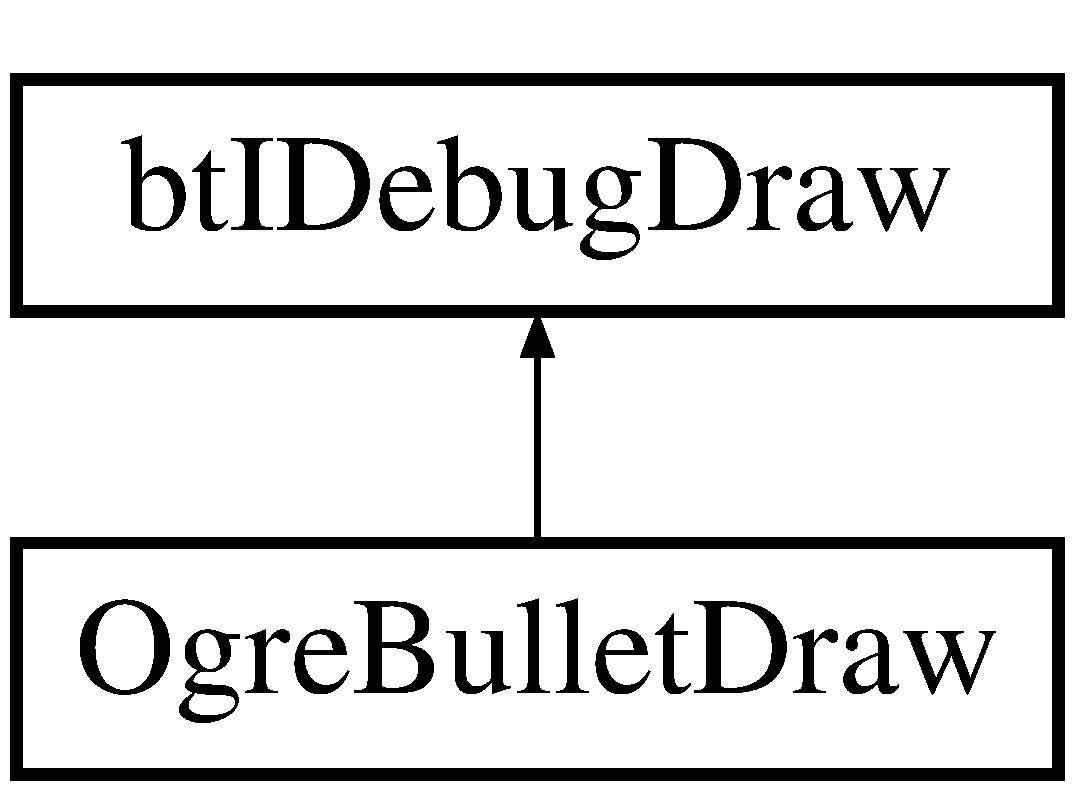
\includegraphics[height=2.000000cm]{class_ogre_bullet_draw}
\end{center}
\end{figure}
\subsection*{Public Member Functions}
\begin{DoxyCompactItemize}
\item 
\hyperlink{class_ogre_bullet_draw_a9c4103fcc420fe9b69cb9d74f8e8e547}{Ogre\-Bullet\-Draw} ()
\begin{DoxyCompactList}\small\item\em Default constructor. \end{DoxyCompactList}\item 
virtual \hyperlink{class_ogre_bullet_draw_acf45d6e54ea76ce26bca1cd8db4afb9f}{$\sim$\-Ogre\-Bullet\-Draw} ()
\begin{DoxyCompactList}\small\item\em Destructor. \end{DoxyCompactList}\item 
virtual void \hyperlink{class_ogre_bullet_draw_a98ce833b82367cfa3233d47d9350995b}{draw\-Line} (const bt\-Vector3 \&from, const bt\-Vector3 \&to, const bt\-Vector3 \&from\-Color, const bt\-Vector3 \&to\-Color)
\begin{DoxyCompactList}\small\item\em Draw line. \end{DoxyCompactList}\item 
virtual void \hyperlink{class_ogre_bullet_draw_ae4a737c479e71935dbd5483763adc299}{draw\-Line} (const bt\-Vector3 \&from, const bt\-Vector3 \&to, const bt\-Vector3 \&color)
\begin{DoxyCompactList}\small\item\em Draw line. \end{DoxyCompactList}\item 
virtual void \hyperlink{class_ogre_bullet_draw_a9be5e64d3202665bb137bbc234457b82}{set\-Debug\-Mode} (int debug\-Mode)
\begin{DoxyCompactList}\small\item\em Sets debug mode. \end{DoxyCompactList}\item 
virtual int \hyperlink{class_ogre_bullet_draw_a7929d3ac3b12030aef451c1c996069c4}{get\-Debug\-Mode} () const 
\begin{DoxyCompactList}\small\item\em Gets debug mode. \end{DoxyCompactList}\item 
virtual void \hyperlink{class_ogre_bullet_draw_add7c437d446cd65f00c600f70707deff}{draw\-Contact\-Point} (const bt\-Vector3 \&Point\-On\-B, const bt\-Vector3 \&normal\-On\-B, bt\-Scalar distance, int life\-Time, const bt\-Vector3 \&color)
\begin{DoxyCompactList}\small\item\em Draw contact point. \end{DoxyCompactList}\item 
virtual void \hyperlink{class_ogre_bullet_draw_a1e0a1e7e892862f415aabcc0eb1b1baf}{report\-Error\-Warning} (const char $\ast$warning\-String)
\begin{DoxyCompactList}\small\item\em Reports error warning. \end{DoxyCompactList}\item 
virtual void \hyperlink{class_ogre_bullet_draw_aeb7f2d2ccce27cb4374190dff6d37e61}{draw3d\-Text} (const bt\-Vector3 \&location, const char $\ast$text\-String)
\begin{DoxyCompactList}\small\item\em Draw 3\-D text. \end{DoxyCompactList}\end{DoxyCompactItemize}


\subsection{Detailed Description}
Ogre bullet draw. 

\begin{DoxyAuthor}{Author}
Arran Ford 
\end{DoxyAuthor}
\begin{DoxyDate}{Date}
31/10/2013 
\end{DoxyDate}


\subsection{Constructor \& Destructor Documentation}
\hypertarget{class_ogre_bullet_draw_a9c4103fcc420fe9b69cb9d74f8e8e547}{\index{Ogre\-Bullet\-Draw@{Ogre\-Bullet\-Draw}!Ogre\-Bullet\-Draw@{Ogre\-Bullet\-Draw}}
\index{Ogre\-Bullet\-Draw@{Ogre\-Bullet\-Draw}!OgreBulletDraw@{Ogre\-Bullet\-Draw}}
\subsubsection[{Ogre\-Bullet\-Draw}]{\setlength{\rightskip}{0pt plus 5cm}Ogre\-Bullet\-Draw\-::\-Ogre\-Bullet\-Draw (
\begin{DoxyParamCaption}
{}
\end{DoxyParamCaption}
)}}\label{class_ogre_bullet_draw_a9c4103fcc420fe9b69cb9d74f8e8e547}


Default constructor. 

\begin{DoxyAuthor}{Author}
Arran Ford 
\end{DoxyAuthor}
\begin{DoxyDate}{Date}
31/10/2013 
\end{DoxyDate}
\hypertarget{class_ogre_bullet_draw_acf45d6e54ea76ce26bca1cd8db4afb9f}{\index{Ogre\-Bullet\-Draw@{Ogre\-Bullet\-Draw}!$\sim$\-Ogre\-Bullet\-Draw@{$\sim$\-Ogre\-Bullet\-Draw}}
\index{$\sim$\-Ogre\-Bullet\-Draw@{$\sim$\-Ogre\-Bullet\-Draw}!OgreBulletDraw@{Ogre\-Bullet\-Draw}}
\subsubsection[{$\sim$\-Ogre\-Bullet\-Draw}]{\setlength{\rightskip}{0pt plus 5cm}Ogre\-Bullet\-Draw\-::$\sim$\-Ogre\-Bullet\-Draw (
\begin{DoxyParamCaption}
{}
\end{DoxyParamCaption}
)\hspace{0.3cm}{\ttfamily [inline]}, {\ttfamily [virtual]}}}\label{class_ogre_bullet_draw_acf45d6e54ea76ce26bca1cd8db4afb9f}


Destructor. 

\begin{DoxyAuthor}{Author}
Arran Ford 
\end{DoxyAuthor}
\begin{DoxyDate}{Date}
31/10/2013 
\end{DoxyDate}


\subsection{Member Function Documentation}
\hypertarget{class_ogre_bullet_draw_aeb7f2d2ccce27cb4374190dff6d37e61}{\index{Ogre\-Bullet\-Draw@{Ogre\-Bullet\-Draw}!draw3d\-Text@{draw3d\-Text}}
\index{draw3d\-Text@{draw3d\-Text}!OgreBulletDraw@{Ogre\-Bullet\-Draw}}
\subsubsection[{draw3d\-Text}]{\setlength{\rightskip}{0pt plus 5cm}void Ogre\-Bullet\-Draw\-::draw3d\-Text (
\begin{DoxyParamCaption}
\item[{const bt\-Vector3 \&}]{location, }
\item[{const char $\ast$}]{text\-String}
\end{DoxyParamCaption}
)\hspace{0.3cm}{\ttfamily [virtual]}}}\label{class_ogre_bullet_draw_aeb7f2d2ccce27cb4374190dff6d37e61}


Draw 3\-D text. 

\begin{DoxyAuthor}{Author}
Arran Ford 
\end{DoxyAuthor}
\begin{DoxyDate}{Date}
31/10/2013
\end{DoxyDate}

\begin{DoxyParams}{Parameters}
{\em location} & The location. \\
\hline
{\em text\-String} & The text string. \\
\hline
\end{DoxyParams}
\hypertarget{class_ogre_bullet_draw_add7c437d446cd65f00c600f70707deff}{\index{Ogre\-Bullet\-Draw@{Ogre\-Bullet\-Draw}!draw\-Contact\-Point@{draw\-Contact\-Point}}
\index{draw\-Contact\-Point@{draw\-Contact\-Point}!OgreBulletDraw@{Ogre\-Bullet\-Draw}}
\subsubsection[{draw\-Contact\-Point}]{\setlength{\rightskip}{0pt plus 5cm}void Ogre\-Bullet\-Draw\-::draw\-Contact\-Point (
\begin{DoxyParamCaption}
\item[{const bt\-Vector3 \&}]{Point\-On\-B, }
\item[{const bt\-Vector3 \&}]{normal\-On\-B, }
\item[{bt\-Scalar}]{distance, }
\item[{int}]{life\-Time, }
\item[{const bt\-Vector3 \&}]{color}
\end{DoxyParamCaption}
)\hspace{0.3cm}{\ttfamily [virtual]}}}\label{class_ogre_bullet_draw_add7c437d446cd65f00c600f70707deff}


Draw contact point. 

\begin{DoxyAuthor}{Author}
Arran Ford 
\end{DoxyAuthor}
\begin{DoxyDate}{Date}
31/10/2013
\end{DoxyDate}

\begin{DoxyParams}{Parameters}
{\em Point\-On\-B} & The point on b. \\
\hline
{\em normal\-On\-B} & The normal on b. \\
\hline
{\em distance} & The distance. \\
\hline
{\em life\-Time} & Time of the life. \\
\hline
{\em color} & The color. \\
\hline
\end{DoxyParams}
\hypertarget{class_ogre_bullet_draw_a98ce833b82367cfa3233d47d9350995b}{\index{Ogre\-Bullet\-Draw@{Ogre\-Bullet\-Draw}!draw\-Line@{draw\-Line}}
\index{draw\-Line@{draw\-Line}!OgreBulletDraw@{Ogre\-Bullet\-Draw}}
\subsubsection[{draw\-Line}]{\setlength{\rightskip}{0pt plus 5cm}void Ogre\-Bullet\-Draw\-::draw\-Line (
\begin{DoxyParamCaption}
\item[{const bt\-Vector3 \&}]{from, }
\item[{const bt\-Vector3 \&}]{to, }
\item[{const bt\-Vector3 \&}]{from\-Color, }
\item[{const bt\-Vector3 \&}]{to\-Color}
\end{DoxyParamCaption}
)\hspace{0.3cm}{\ttfamily [virtual]}}}\label{class_ogre_bullet_draw_a98ce833b82367cfa3233d47d9350995b}


Draw line. 

\begin{DoxyAuthor}{Author}
Arran Ford 
\end{DoxyAuthor}
\begin{DoxyDate}{Date}
31/10/2013
\end{DoxyDate}

\begin{DoxyParams}{Parameters}
{\em from} & Source for the. \\
\hline
{\em to} & to. \\
\hline
{\em from\-Color} & from color. \\
\hline
{\em to\-Color} & to color. \\
\hline
\end{DoxyParams}
\hypertarget{class_ogre_bullet_draw_ae4a737c479e71935dbd5483763adc299}{\index{Ogre\-Bullet\-Draw@{Ogre\-Bullet\-Draw}!draw\-Line@{draw\-Line}}
\index{draw\-Line@{draw\-Line}!OgreBulletDraw@{Ogre\-Bullet\-Draw}}
\subsubsection[{draw\-Line}]{\setlength{\rightskip}{0pt plus 5cm}void Ogre\-Bullet\-Draw\-::draw\-Line (
\begin{DoxyParamCaption}
\item[{const bt\-Vector3 \&}]{from, }
\item[{const bt\-Vector3 \&}]{to, }
\item[{const bt\-Vector3 \&}]{color}
\end{DoxyParamCaption}
)\hspace{0.3cm}{\ttfamily [virtual]}}}\label{class_ogre_bullet_draw_ae4a737c479e71935dbd5483763adc299}


Draw line. 

\begin{DoxyAuthor}{Author}
Arran Ford 
\end{DoxyAuthor}
\begin{DoxyDate}{Date}
31/10/2013
\end{DoxyDate}

\begin{DoxyParams}{Parameters}
{\em from} & Source for the. \\
\hline
{\em to} & to. \\
\hline
{\em color} & The color. \\
\hline
\end{DoxyParams}
\hypertarget{class_ogre_bullet_draw_a7929d3ac3b12030aef451c1c996069c4}{\index{Ogre\-Bullet\-Draw@{Ogre\-Bullet\-Draw}!get\-Debug\-Mode@{get\-Debug\-Mode}}
\index{get\-Debug\-Mode@{get\-Debug\-Mode}!OgreBulletDraw@{Ogre\-Bullet\-Draw}}
\subsubsection[{get\-Debug\-Mode}]{\setlength{\rightskip}{0pt plus 5cm}int Ogre\-Bullet\-Draw\-::get\-Debug\-Mode (
\begin{DoxyParamCaption}
{}
\end{DoxyParamCaption}
) const\hspace{0.3cm}{\ttfamily [inline]}, {\ttfamily [virtual]}}}\label{class_ogre_bullet_draw_a7929d3ac3b12030aef451c1c996069c4}


Gets debug mode. 

\begin{DoxyAuthor}{Author}
Arran Ford 
\end{DoxyAuthor}
\begin{DoxyDate}{Date}
31/10/2013
\end{DoxyDate}
\begin{DoxyReturn}{Returns}
The debug mode. 
\end{DoxyReturn}
\hypertarget{class_ogre_bullet_draw_a1e0a1e7e892862f415aabcc0eb1b1baf}{\index{Ogre\-Bullet\-Draw@{Ogre\-Bullet\-Draw}!report\-Error\-Warning@{report\-Error\-Warning}}
\index{report\-Error\-Warning@{report\-Error\-Warning}!OgreBulletDraw@{Ogre\-Bullet\-Draw}}
\subsubsection[{report\-Error\-Warning}]{\setlength{\rightskip}{0pt plus 5cm}void Ogre\-Bullet\-Draw\-::report\-Error\-Warning (
\begin{DoxyParamCaption}
\item[{const char $\ast$}]{warning\-String}
\end{DoxyParamCaption}
)\hspace{0.3cm}{\ttfamily [virtual]}}}\label{class_ogre_bullet_draw_a1e0a1e7e892862f415aabcc0eb1b1baf}


Reports error warning. 

\begin{DoxyAuthor}{Author}
Arran Ford 
\end{DoxyAuthor}
\begin{DoxyDate}{Date}
31/10/2013
\end{DoxyDate}

\begin{DoxyParams}{Parameters}
{\em warning\-String} & The warning string. \\
\hline
\end{DoxyParams}
\hypertarget{class_ogre_bullet_draw_a9be5e64d3202665bb137bbc234457b82}{\index{Ogre\-Bullet\-Draw@{Ogre\-Bullet\-Draw}!set\-Debug\-Mode@{set\-Debug\-Mode}}
\index{set\-Debug\-Mode@{set\-Debug\-Mode}!OgreBulletDraw@{Ogre\-Bullet\-Draw}}
\subsubsection[{set\-Debug\-Mode}]{\setlength{\rightskip}{0pt plus 5cm}void Ogre\-Bullet\-Draw\-::set\-Debug\-Mode (
\begin{DoxyParamCaption}
\item[{int}]{debug\-Mode}
\end{DoxyParamCaption}
)\hspace{0.3cm}{\ttfamily [virtual]}}}\label{class_ogre_bullet_draw_a9be5e64d3202665bb137bbc234457b82}


Sets debug mode. 

\begin{DoxyAuthor}{Author}
Arran Ford 
\end{DoxyAuthor}
\begin{DoxyDate}{Date}
31/10/2013
\end{DoxyDate}

\begin{DoxyParams}{Parameters}
{\em debug\-Mode} & The debug mode. \\
\hline
\end{DoxyParams}


The documentation for this class was generated from the following files\-:\begin{DoxyCompactItemize}
\item 
A\-:/\-I\-T/\-Git\-Hub/\-I\-C\-T312/source/ogregraphics/\hyperlink{_ogre_bullet_draw_8h}{Ogre\-Bullet\-Draw.\-h}\item 
A\-:/\-I\-T/\-Git\-Hub/\-I\-C\-T312/source/ogregraphics/Ogre\-Bullet\-Draw.\-cpp\end{DoxyCompactItemize}

\hypertarget{class_ogre_debug_drawer}{\section{Ogre\-Debug\-Drawer Class Reference}
\label{class_ogre_debug_drawer}\index{Ogre\-Debug\-Drawer@{Ogre\-Debug\-Drawer}}
}
Inheritance diagram for Ogre\-Debug\-Drawer\-:\begin{figure}[H]
\begin{center}
\leavevmode
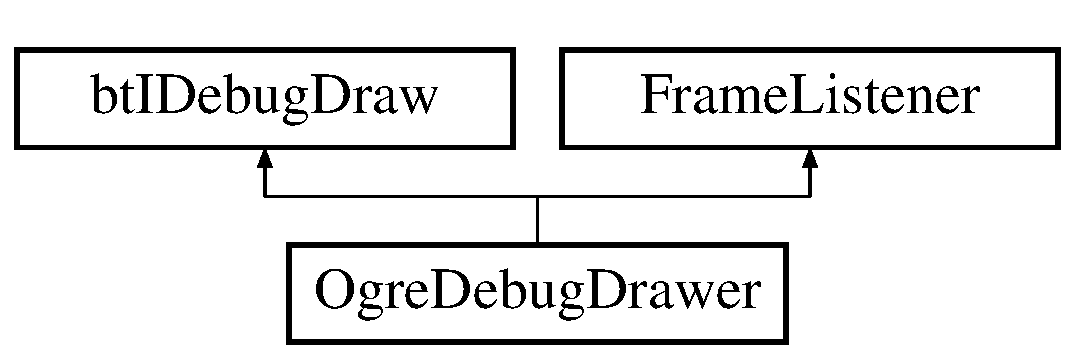
\includegraphics[height=2.000000cm]{class_ogre_debug_drawer}
\end{center}
\end{figure}
\subsection*{Public Member Functions}
\begin{DoxyCompactItemize}
\item 
\hyperlink{class_ogre_debug_drawer_affa9afb5fe47e691f51f9e3f8b6bfc06}{Ogre\-Debug\-Drawer} (Ogre\-::\-Scene\-Manager $\ast$scm)
\begin{DoxyCompactList}\small\item\em Constructor. \end{DoxyCompactList}\item 
\hyperlink{class_ogre_debug_drawer_a7fb8d446130457b47e47c5f5ee6a7a43}{$\sim$\-Ogre\-Debug\-Drawer} ()
\begin{DoxyCompactList}\small\item\em Destructor. \end{DoxyCompactList}\item 
virtual void \hyperlink{class_ogre_debug_drawer_a8086cc1f589d77cb7c8ca40d0238e91d}{draw\-Line} (const bt\-Vector3 \&from, const bt\-Vector3 \&to, const bt\-Vector3 \&color)
\begin{DoxyCompactList}\small\item\em Draw line. \end{DoxyCompactList}\item 
virtual void \hyperlink{class_ogre_debug_drawer_aec9e358cee25c958f012d44c224af1dc}{draw\-Triangle} (const bt\-Vector3 \&v0, const bt\-Vector3 \&v1, const bt\-Vector3 \&v2, const bt\-Vector3 \&color, bt\-Scalar)
\begin{DoxyCompactList}\small\item\em Draw triangle. \end{DoxyCompactList}\item 
virtual void \hyperlink{class_ogre_debug_drawer_ad7c599acc8ccd6bef42d4178775ed56b}{draw\-Contact\-Point} (const bt\-Vector3 \&Point\-On\-B, const bt\-Vector3 \&normal\-On\-B, bt\-Scalar distance, int life\-Time, const bt\-Vector3 \&color)
\begin{DoxyCompactList}\small\item\em Draw contact point. \end{DoxyCompactList}\item 
virtual void \hyperlink{class_ogre_debug_drawer_a8ae828583fcb82103c3ba8525448abff}{report\-Error\-Warning} (const char $\ast$warning\-String)
\begin{DoxyCompactList}\small\item\em Reports error warning. \end{DoxyCompactList}\item 
virtual void \hyperlink{class_ogre_debug_drawer_aad49212d18a6498510ec7ce685387e30}{draw3d\-Text} (const bt\-Vector3 \&location, const char $\ast$text\-String)
\begin{DoxyCompactList}\small\item\em Draw 3\-D text. \end{DoxyCompactList}\item 
virtual void \hyperlink{class_ogre_debug_drawer_afadea9d4ff16871d8a07408246dedb6f}{set\-Debug\-Mode} (int debug\-Mode)
\begin{DoxyCompactList}\small\item\em Sets debug mode. \end{DoxyCompactList}\item 
virtual int \hyperlink{class_ogre_debug_drawer_add90fea7be402da9507604ca1f3b9cb1}{get\-Debug\-Mode} () const 
\begin{DoxyCompactList}\small\item\em Gets debug mode. \end{DoxyCompactList}\end{DoxyCompactItemize}
\subsection*{Protected Member Functions}
\begin{DoxyCompactItemize}
\item 
bool \hyperlink{class_ogre_debug_drawer_a7f72263ebfeac05793ad21a76ac22130}{frame\-Started} (const Ogre\-::\-Frame\-Event \&evt)
\begin{DoxyCompactList}\small\item\em Frame started. \end{DoxyCompactList}\item 
bool \hyperlink{class_ogre_debug_drawer_adefa1752a3968fc2f156fa14a4b3fe76}{frame\-Ended} (const Ogre\-::\-Frame\-Event \&evt)
\begin{DoxyCompactList}\small\item\em Frame ended. \end{DoxyCompactList}\end{DoxyCompactItemize}


\subsection{Constructor \& Destructor Documentation}
\hypertarget{class_ogre_debug_drawer_affa9afb5fe47e691f51f9e3f8b6bfc06}{\index{Ogre\-Debug\-Drawer@{Ogre\-Debug\-Drawer}!Ogre\-Debug\-Drawer@{Ogre\-Debug\-Drawer}}
\index{Ogre\-Debug\-Drawer@{Ogre\-Debug\-Drawer}!OgreDebugDrawer@{Ogre\-Debug\-Drawer}}
\subsubsection[{Ogre\-Debug\-Drawer}]{\setlength{\rightskip}{0pt plus 5cm}Ogre\-Debug\-Drawer\-::\-Ogre\-Debug\-Drawer (
\begin{DoxyParamCaption}
\item[{Ogre\-::\-Scene\-Manager $\ast$}]{scm}
\end{DoxyParamCaption}
)}}\label{class_ogre_debug_drawer_affa9afb5fe47e691f51f9e3f8b6bfc06}


Constructor. 

\begin{DoxyAuthor}{Author}
Ogre Wiki 
\end{DoxyAuthor}
\begin{DoxyDate}{Date}
31/10/2013
\end{DoxyDate}

\begin{DoxyParams}[1]{Parameters}
\mbox{\tt in,out}  & {\em scm} & If non-\/null, the scm. \\
\hline
\end{DoxyParams}
\hypertarget{class_ogre_debug_drawer_a7fb8d446130457b47e47c5f5ee6a7a43}{\index{Ogre\-Debug\-Drawer@{Ogre\-Debug\-Drawer}!$\sim$\-Ogre\-Debug\-Drawer@{$\sim$\-Ogre\-Debug\-Drawer}}
\index{$\sim$\-Ogre\-Debug\-Drawer@{$\sim$\-Ogre\-Debug\-Drawer}!OgreDebugDrawer@{Ogre\-Debug\-Drawer}}
\subsubsection[{$\sim$\-Ogre\-Debug\-Drawer}]{\setlength{\rightskip}{0pt plus 5cm}Ogre\-Debug\-Drawer\-::$\sim$\-Ogre\-Debug\-Drawer (
\begin{DoxyParamCaption}
{}
\end{DoxyParamCaption}
)}}\label{class_ogre_debug_drawer_a7fb8d446130457b47e47c5f5ee6a7a43}


Destructor. 

\begin{DoxyAuthor}{Author}
Ogre Wiki 
\end{DoxyAuthor}
\begin{DoxyDate}{Date}
31/10/2013 
\end{DoxyDate}


\subsection{Member Function Documentation}
\hypertarget{class_ogre_debug_drawer_aad49212d18a6498510ec7ce685387e30}{\index{Ogre\-Debug\-Drawer@{Ogre\-Debug\-Drawer}!draw3d\-Text@{draw3d\-Text}}
\index{draw3d\-Text@{draw3d\-Text}!OgreDebugDrawer@{Ogre\-Debug\-Drawer}}
\subsubsection[{draw3d\-Text}]{\setlength{\rightskip}{0pt plus 5cm}void Ogre\-Debug\-Drawer\-::draw3d\-Text (
\begin{DoxyParamCaption}
\item[{const bt\-Vector3 \&}]{location, }
\item[{const char $\ast$}]{text\-String}
\end{DoxyParamCaption}
)\hspace{0.3cm}{\ttfamily [virtual]}}}\label{class_ogre_debug_drawer_aad49212d18a6498510ec7ce685387e30}


Draw 3\-D text. 

\begin{DoxyAuthor}{Author}
Ogre Wiki 
\end{DoxyAuthor}
\begin{DoxyDate}{Date}
31/10/2013
\end{DoxyDate}

\begin{DoxyParams}{Parameters}
{\em location} & The location. \\
\hline
{\em text\-String} & The text string. \\
\hline
\end{DoxyParams}
\hypertarget{class_ogre_debug_drawer_ad7c599acc8ccd6bef42d4178775ed56b}{\index{Ogre\-Debug\-Drawer@{Ogre\-Debug\-Drawer}!draw\-Contact\-Point@{draw\-Contact\-Point}}
\index{draw\-Contact\-Point@{draw\-Contact\-Point}!OgreDebugDrawer@{Ogre\-Debug\-Drawer}}
\subsubsection[{draw\-Contact\-Point}]{\setlength{\rightskip}{0pt plus 5cm}void Ogre\-Debug\-Drawer\-::draw\-Contact\-Point (
\begin{DoxyParamCaption}
\item[{const bt\-Vector3 \&}]{Point\-On\-B, }
\item[{const bt\-Vector3 \&}]{normal\-On\-B, }
\item[{bt\-Scalar}]{distance, }
\item[{int}]{life\-Time, }
\item[{const bt\-Vector3 \&}]{color}
\end{DoxyParamCaption}
)\hspace{0.3cm}{\ttfamily [virtual]}}}\label{class_ogre_debug_drawer_ad7c599acc8ccd6bef42d4178775ed56b}


Draw contact point. 

\begin{DoxyAuthor}{Author}
Ogre Wiki 
\end{DoxyAuthor}
\begin{DoxyDate}{Date}
31/10/2013
\end{DoxyDate}

\begin{DoxyParams}{Parameters}
{\em Point\-On\-B} & The point on b. \\
\hline
{\em normal\-On\-B} & The normal on b. \\
\hline
{\em distance} & The distance. \\
\hline
{\em life\-Time} & Time of the life. \\
\hline
{\em color} & The color. \\
\hline
\end{DoxyParams}
\hypertarget{class_ogre_debug_drawer_a8086cc1f589d77cb7c8ca40d0238e91d}{\index{Ogre\-Debug\-Drawer@{Ogre\-Debug\-Drawer}!draw\-Line@{draw\-Line}}
\index{draw\-Line@{draw\-Line}!OgreDebugDrawer@{Ogre\-Debug\-Drawer}}
\subsubsection[{draw\-Line}]{\setlength{\rightskip}{0pt plus 5cm}void Ogre\-Debug\-Drawer\-::draw\-Line (
\begin{DoxyParamCaption}
\item[{const bt\-Vector3 \&}]{from, }
\item[{const bt\-Vector3 \&}]{to, }
\item[{const bt\-Vector3 \&}]{color}
\end{DoxyParamCaption}
)\hspace{0.3cm}{\ttfamily [virtual]}}}\label{class_ogre_debug_drawer_a8086cc1f589d77cb7c8ca40d0238e91d}


Draw line. 

\begin{DoxyAuthor}{Author}
Ogre Wiki 
\end{DoxyAuthor}
\begin{DoxyDate}{Date}
31/10/2013
\end{DoxyDate}

\begin{DoxyParams}{Parameters}
{\em from} & Source for the. \\
\hline
{\em to} & to. \\
\hline
{\em color} & The color. \\
\hline
\end{DoxyParams}
\hypertarget{class_ogre_debug_drawer_aec9e358cee25c958f012d44c224af1dc}{\index{Ogre\-Debug\-Drawer@{Ogre\-Debug\-Drawer}!draw\-Triangle@{draw\-Triangle}}
\index{draw\-Triangle@{draw\-Triangle}!OgreDebugDrawer@{Ogre\-Debug\-Drawer}}
\subsubsection[{draw\-Triangle}]{\setlength{\rightskip}{0pt plus 5cm}void Ogre\-Debug\-Drawer\-::draw\-Triangle (
\begin{DoxyParamCaption}
\item[{const bt\-Vector3 \&}]{v0, }
\item[{const bt\-Vector3 \&}]{v1, }
\item[{const bt\-Vector3 \&}]{v2, }
\item[{const bt\-Vector3 \&}]{color, }
\item[{bt\-Scalar}]{alpha}
\end{DoxyParamCaption}
)\hspace{0.3cm}{\ttfamily [virtual]}}}\label{class_ogre_debug_drawer_aec9e358cee25c958f012d44c224af1dc}


Draw triangle. 

\begin{DoxyAuthor}{Author}
Ogre Wiki 
\end{DoxyAuthor}
\begin{DoxyDate}{Date}
31/10/2013
\end{DoxyDate}

\begin{DoxyParams}{Parameters}
{\em v0} & The v 0. \\
\hline
{\em v1} & The first bt\-Vector3. \\
\hline
{\em v2} & The second bt\-Vector3. \\
\hline
{\em color} & The color. \\
\hline
{\em parameter5} & The fifth parameter. \\
\hline
\end{DoxyParams}
\hypertarget{class_ogre_debug_drawer_adefa1752a3968fc2f156fa14a4b3fe76}{\index{Ogre\-Debug\-Drawer@{Ogre\-Debug\-Drawer}!frame\-Ended@{frame\-Ended}}
\index{frame\-Ended@{frame\-Ended}!OgreDebugDrawer@{Ogre\-Debug\-Drawer}}
\subsubsection[{frame\-Ended}]{\setlength{\rightskip}{0pt plus 5cm}bool Ogre\-Debug\-Drawer\-::frame\-Ended (
\begin{DoxyParamCaption}
\item[{const Ogre\-::\-Frame\-Event \&}]{evt}
\end{DoxyParamCaption}
)\hspace{0.3cm}{\ttfamily [protected]}}}\label{class_ogre_debug_drawer_adefa1752a3968fc2f156fa14a4b3fe76}


Frame ended. 

\begin{DoxyAuthor}{Author}
Ogre Wiki 
\end{DoxyAuthor}
\begin{DoxyDate}{Date}
31/10/2013
\end{DoxyDate}

\begin{DoxyParams}{Parameters}
{\em evt} & The event.\\
\hline
\end{DoxyParams}
\begin{DoxyReturn}{Returns}
true if it succeeds, false if it fails. 
\end{DoxyReturn}
\hypertarget{class_ogre_debug_drawer_a7f72263ebfeac05793ad21a76ac22130}{\index{Ogre\-Debug\-Drawer@{Ogre\-Debug\-Drawer}!frame\-Started@{frame\-Started}}
\index{frame\-Started@{frame\-Started}!OgreDebugDrawer@{Ogre\-Debug\-Drawer}}
\subsubsection[{frame\-Started}]{\setlength{\rightskip}{0pt plus 5cm}bool Ogre\-Debug\-Drawer\-::frame\-Started (
\begin{DoxyParamCaption}
\item[{const Ogre\-::\-Frame\-Event \&}]{evt}
\end{DoxyParamCaption}
)\hspace{0.3cm}{\ttfamily [protected]}}}\label{class_ogre_debug_drawer_a7f72263ebfeac05793ad21a76ac22130}


Frame started. 

\begin{DoxyAuthor}{Author}
Ogre Wiki 
\end{DoxyAuthor}
\begin{DoxyDate}{Date}
31/10/2013
\end{DoxyDate}

\begin{DoxyParams}{Parameters}
{\em evt} & The event.\\
\hline
\end{DoxyParams}
\begin{DoxyReturn}{Returns}
true if it succeeds, false if it fails. 
\end{DoxyReturn}
\hypertarget{class_ogre_debug_drawer_add90fea7be402da9507604ca1f3b9cb1}{\index{Ogre\-Debug\-Drawer@{Ogre\-Debug\-Drawer}!get\-Debug\-Mode@{get\-Debug\-Mode}}
\index{get\-Debug\-Mode@{get\-Debug\-Mode}!OgreDebugDrawer@{Ogre\-Debug\-Drawer}}
\subsubsection[{get\-Debug\-Mode}]{\setlength{\rightskip}{0pt plus 5cm}int Ogre\-Debug\-Drawer\-::get\-Debug\-Mode (
\begin{DoxyParamCaption}
{}
\end{DoxyParamCaption}
) const\hspace{0.3cm}{\ttfamily [virtual]}}}\label{class_ogre_debug_drawer_add90fea7be402da9507604ca1f3b9cb1}


Gets debug mode. 

\begin{DoxyAuthor}{Author}
Ogre Wiki 
\end{DoxyAuthor}
\begin{DoxyDate}{Date}
31/10/2013
\end{DoxyDate}
\begin{DoxyReturn}{Returns}
The debug mode. 
\end{DoxyReturn}
\hypertarget{class_ogre_debug_drawer_a8ae828583fcb82103c3ba8525448abff}{\index{Ogre\-Debug\-Drawer@{Ogre\-Debug\-Drawer}!report\-Error\-Warning@{report\-Error\-Warning}}
\index{report\-Error\-Warning@{report\-Error\-Warning}!OgreDebugDrawer@{Ogre\-Debug\-Drawer}}
\subsubsection[{report\-Error\-Warning}]{\setlength{\rightskip}{0pt plus 5cm}void Ogre\-Debug\-Drawer\-::report\-Error\-Warning (
\begin{DoxyParamCaption}
\item[{const char $\ast$}]{warning\-String}
\end{DoxyParamCaption}
)\hspace{0.3cm}{\ttfamily [virtual]}}}\label{class_ogre_debug_drawer_a8ae828583fcb82103c3ba8525448abff}


Reports error warning. 

\begin{DoxyAuthor}{Author}
Ogre Wiki 
\end{DoxyAuthor}
\begin{DoxyDate}{Date}
31/10/2013
\end{DoxyDate}

\begin{DoxyParams}{Parameters}
{\em warning\-String} & The warning string. \\
\hline
\end{DoxyParams}
\hypertarget{class_ogre_debug_drawer_afadea9d4ff16871d8a07408246dedb6f}{\index{Ogre\-Debug\-Drawer@{Ogre\-Debug\-Drawer}!set\-Debug\-Mode@{set\-Debug\-Mode}}
\index{set\-Debug\-Mode@{set\-Debug\-Mode}!OgreDebugDrawer@{Ogre\-Debug\-Drawer}}
\subsubsection[{set\-Debug\-Mode}]{\setlength{\rightskip}{0pt plus 5cm}void Ogre\-Debug\-Drawer\-::set\-Debug\-Mode (
\begin{DoxyParamCaption}
\item[{int}]{debug\-Mode}
\end{DoxyParamCaption}
)\hspace{0.3cm}{\ttfamily [virtual]}}}\label{class_ogre_debug_drawer_afadea9d4ff16871d8a07408246dedb6f}


Sets debug mode. 

\begin{DoxyAuthor}{Author}
Ogre Wiki 
\end{DoxyAuthor}
\begin{DoxyDate}{Date}
31/10/2013
\end{DoxyDate}

\begin{DoxyParams}{Parameters}
{\em debug\-Mode} & The debug mode. \\
\hline
\end{DoxyParams}


The documentation for this class was generated from the following files\-:\begin{DoxyCompactItemize}
\item 
A\-:/\-I\-T/\-Git\-Hub/\-I\-C\-T312/source/ogregraphics/\hyperlink{_debug_drawer_og_8h}{Debug\-Drawer\-Og.\-h}\item 
A\-:/\-I\-T/\-Git\-Hub/\-I\-C\-T312/source/ogregraphics/Debug\-Drawer\-Og.\-cpp\end{DoxyCompactItemize}

\hypertarget{class_graphics_1_1_ogre_graphics}{\section{Graphics\-:\-:Ogre\-Graphics Class Reference}
\label{class_graphics_1_1_ogre_graphics}\index{Graphics\-::\-Ogre\-Graphics@{Graphics\-::\-Ogre\-Graphics}}
}


Facade class for Ogre3\-D graphics engine. Allows for the creation of windows, cameras, lighting, entities and more using Ogre3\-D.  




{\ttfamily \#include $<$Ogre\-Graphics.\-h$>$}

\subsection*{Public Member Functions}
\begin{DoxyCompactItemize}
\item 
\hypertarget{class_graphics_1_1_ogre_graphics_a37c6b9f85aa0ce9f8c8d04db516a5371}{Ogre\-::\-Vector3 {\bfseries Get\-Position} ()}\label{class_graphics_1_1_ogre_graphics_a37c6b9f85aa0ce9f8c8d04db516a5371}

\item 
\hyperlink{class_graphics_1_1_ogre_graphics_a007a31a8efc2475971a6c3f432ea640f}{Ogre\-Graphics} (void)
\begin{DoxyCompactList}\small\item\em Default constructor. \end{DoxyCompactList}\item 
\hyperlink{class_graphics_1_1_ogre_graphics_a019747c24e5a65f0a3ccab895c09c6f7}{$\sim$\-Ogre\-Graphics} (void)
\begin{DoxyCompactList}\small\item\em Destructor. \end{DoxyCompactList}\item 
bool \hyperlink{class_graphics_1_1_ogre_graphics_a90de3a0bb9efe9b94ca1d97d6bae4e48}{initialise} ()
\begin{DoxyCompactList}\small\item\em Initialises this object. \end{DoxyCompactList}\item 
void \hyperlink{class_graphics_1_1_ogre_graphics_aa76873367c5bb0f08add8f25ee1a6ee3}{load\-Resources} ()
\begin{DoxyCompactList}\small\item\em Loads the resources. \end{DoxyCompactList}\item 
void \hyperlink{class_graphics_1_1_ogre_graphics_a8f681b4e4564949b88e25803d70302ed}{render\-One\-Frame} ()
\begin{DoxyCompactList}\small\item\em Renders a single frame. \end{DoxyCompactList}\item 
float \hyperlink{class_graphics_1_1_ogre_graphics_a28e230d27cc293d46e0672cd741050bf}{get\-Delta\-Time} ()
\begin{DoxyCompactList}\small\item\em Gets delta time. \end{DoxyCompactList}\item 
void \hyperlink{class_graphics_1_1_ogre_graphics_a45c7525b6fb3599127301d27ffc25999}{camera\-Set\-Position} (float pos\-X, float pos\-Y, float pos\-Z)
\begin{DoxyCompactList}\small\item\em Sets the position of the camera object. \end{DoxyCompactList}\item 
void \hyperlink{class_graphics_1_1_ogre_graphics_a167d450f5072b96560f1c56892403243}{camera\-Set\-Look\-At} (float look\-At\-X, float look\-At\-Y, float look\-At\-Z)
\begin{DoxyCompactList}\small\item\em Sets the point that the camera object looks at. \end{DoxyCompactList}\item 
void \hyperlink{class_graphics_1_1_ogre_graphics_aae212ac2be0588b2b977d64ba4b33746}{camera\-Set\-Aspect\-Ratio} (float ratio)
\begin{DoxyCompactList}\small\item\em Sets the aspect ratio from which the camera is viewed. \end{DoxyCompactList}\item 
void \hyperlink{class_graphics_1_1_ogre_graphics_ac9a3f3eec14d2a5b6d767696f70198ed}{camera\-Move\-Relative} (Ogre\-::\-Vector3 \&movement)
\begin{DoxyCompactList}\small\item\em Moves the camera object relative to its current position. \end{DoxyCompactList}\item 
void \hyperlink{class_graphics_1_1_ogre_graphics_a81de9be1c14e6f5b4ea8e7343a0725e0}{camera\-Yaw} (Ogre\-::\-Radian \&angle)
\begin{DoxyCompactList}\small\item\em Sets the camera yaw angle. \end{DoxyCompactList}\item 
void \hyperlink{class_graphics_1_1_ogre_graphics_a00ef565a1cf666f72808d327fb0ff533}{camera\-Pitch} (Ogre\-::\-Radian \&angle)
\begin{DoxyCompactList}\small\item\em Sets the camera pitch angle. \end{DoxyCompactList}\item 
\hypertarget{class_graphics_1_1_ogre_graphics_a64f51c4ae82086c83f393b4481bbc2e6}{Ogre\-::\-Vector3 {\bfseries camera\-Direction} ()}\label{class_graphics_1_1_ogre_graphics_a64f51c4ae82086c83f393b4481bbc2e6}

\item 
int \hyperlink{class_graphics_1_1_ogre_graphics_a499281e2495fa88c0608a10e4114e3e9}{get\-Window\-Width} () const 
\begin{DoxyCompactList}\small\item\em Returns the width of the window. \end{DoxyCompactList}\item 
int \hyperlink{class_graphics_1_1_ogre_graphics_a4bcd073336c76de1b27129247c52f1da}{get\-Window\-Height} () const 
\begin{DoxyCompactList}\small\item\em Returns the height of the window. \end{DoxyCompactList}\item 
Ogre\-::\-Render\-Window $\ast$ \hyperlink{class_graphics_1_1_ogre_graphics_a0bd9f35fabd4e8cf3c505205d35e1168}{get\-Render\-Window} () const 
\begin{DoxyCompactList}\small\item\em Gets render window. T\-O\-D\-O\-: Remove in favor of outputting the necessary information. \end{DoxyCompactList}\item 
void \hyperlink{class_graphics_1_1_ogre_graphics_a7f411e7b4427d0f7bb4250383de4863d}{create\-Mesh\-Entity} (std\-::string identifier, std\-::string filename)
\begin{DoxyCompactList}\small\item\em Creates a mesh entity and attaches it to the root scene node. \end{DoxyCompactList}\item 
void \hyperlink{class_graphics_1_1_ogre_graphics_a36baf8b52d4d674ebdb07690482f5206}{create\-Plane\-Entity} (std\-::string identifier, std\-::string mesh\-Name, Ogre\-::\-Vector3 normal, float change\-Along\-Normal, float width, float height, int x\-Segments, int y\-Segments, float u\-Tile, float v\-Tile, std\-::string material=N\-U\-L\-L)
\begin{DoxyCompactList}\small\item\em Creates plane entity and attaches it to the root scene node. \end{DoxyCompactList}\item 
void \hyperlink{class_graphics_1_1_ogre_graphics_af9e33ddceec43e569f6661e0b97362f2}{create\-Directional\-Light} (std\-::string name, float pos\-X, float pos\-Y, float pos\-Z, float dir\-X, float dir\-Y, float dir\-Z)
\begin{DoxyCompactList}\small\item\em Creates a directional light at the position specified facing in the input direction. \end{DoxyCompactList}\item 
\hypertarget{class_graphics_1_1_ogre_graphics_aef364c5496904a81976882440b42ff0f}{void {\bfseries create\-Empty\-Entity} (std\-::string identifier)}\label{class_graphics_1_1_ogre_graphics_aef364c5496904a81976882440b42ff0f}

\item 
\hypertarget{class_graphics_1_1_ogre_graphics_a9bd41a31f524415fbf24f4afdfa6b849}{void {\bfseries create\-Child\-Entity} (std\-::string parent\-I\-D, std\-::string child\-I\-D)}\label{class_graphics_1_1_ogre_graphics_a9bd41a31f524415fbf24f4afdfa6b849}

\item 
\hypertarget{class_graphics_1_1_ogre_graphics_a7b47035683126a79b25339b047760c40}{void {\bfseries set\-Entity\-Yaw} (std\-::string identifier, float angle)}\label{class_graphics_1_1_ogre_graphics_a7b47035683126a79b25339b047760c40}

\item 
\hypertarget{class_graphics_1_1_ogre_graphics_abb152e52376d33197737153111d6a471}{void {\bfseries set\-Entity\-Pitch} (std\-::string identifier, float angle)}\label{class_graphics_1_1_ogre_graphics_abb152e52376d33197737153111d6a471}

\item 
\hypertarget{class_graphics_1_1_ogre_graphics_abe3417c9678ae99406c1b4fe8f657d23}{void {\bfseries set\-Entity\-Roll} (std\-::string identifier, float angle)}\label{class_graphics_1_1_ogre_graphics_abe3417c9678ae99406c1b4fe8f657d23}

\item 
\hypertarget{class_graphics_1_1_ogre_graphics_a6b2182aa52386a6acb9c562ed06f2995}{void {\bfseries translate\-Entity} (std\-::string identifier, float x, float y, float z)}\label{class_graphics_1_1_ogre_graphics_a6b2182aa52386a6acb9c562ed06f2995}

\item 
\hypertarget{class_graphics_1_1_ogre_graphics_a846ccf667116effe488c937fd887aa74}{void {\bfseries translate\-Entity} (std\-::string identifier, Ogre\-::\-Vector3 translate\-Vector)}\label{class_graphics_1_1_ogre_graphics_a846ccf667116effe488c937fd887aa74}

\item 
\hypertarget{class_graphics_1_1_ogre_graphics_a3a7362473ed9c51c27dabf961153795b}{void {\bfseries set\-Entity\-Position} (std\-::string identifier, float x, float y, float z)}\label{class_graphics_1_1_ogre_graphics_a3a7362473ed9c51c27dabf961153795b}

\item 
\hypertarget{class_graphics_1_1_ogre_graphics_a16a9ba92da6e659660b31aca768e94ab}{Ogre\-::\-Quaternion {\bfseries get\-Entity\-Orientation} (std\-::string identifier)}\label{class_graphics_1_1_ogre_graphics_a16a9ba92da6e659660b31aca768e94ab}

\item 
\hypertarget{class_graphics_1_1_ogre_graphics_aaf5e3542879b6ccafdd40facb3cd12d6}{void {\bfseries set\-Entity\-Orientation} (std\-::string identifier, Ogre\-::\-Quaternion quat)}\label{class_graphics_1_1_ogre_graphics_aaf5e3542879b6ccafdd40facb3cd12d6}

\item 
\hypertarget{class_graphics_1_1_ogre_graphics_a80abd401399f859017ff78f40b11fdd8}{void {\bfseries set\-Entity\-Scale} (std\-::string identifier, Ogre\-::\-Vector3 scale)}\label{class_graphics_1_1_ogre_graphics_a80abd401399f859017ff78f40b11fdd8}

\item 
\hypertarget{class_graphics_1_1_ogre_graphics_a0bf286f46a9204675ff257104169cc89}{Ogre\-::\-Vector3 {\bfseries get\-Entity\-Scale} (std\-::string identifier)}\label{class_graphics_1_1_ogre_graphics_a0bf286f46a9204675ff257104169cc89}

\item 
\hypertarget{class_graphics_1_1_ogre_graphics_a7936afa4e8d5078c4f2f1dd2912c639c}{Ogre\-::\-Entity $\ast$ {\bfseries get\-Entity} (std\-::string identifier)}\label{class_graphics_1_1_ogre_graphics_a7936afa4e8d5078c4f2f1dd2912c639c}

\item 
\hypertarget{class_graphics_1_1_ogre_graphics_abbddf0740d07b37ab2c4d93d2f87758a}{\hyperlink{class_debug_drawer}{Debug\-Drawer} $\ast$ {\bfseries get\-Debug\-Drawer} ()}\label{class_graphics_1_1_ogre_graphics_abbddf0740d07b37ab2c4d93d2f87758a}

\item 
\hypertarget{class_graphics_1_1_ogre_graphics_a887b5276d28309a584421d1658a67666}{Ogre\-::\-Scene\-Manager $\ast$ {\bfseries Get\-Scene\-Manager} ()}\label{class_graphics_1_1_ogre_graphics_a887b5276d28309a584421d1658a67666}

\end{DoxyCompactItemize}


\subsection{Detailed Description}
Facade class for Ogre3\-D graphics engine. Allows for the creation of windows, cameras, lighting, entities and more using Ogre3\-D. 

\begin{DoxyAuthor}{Author}
Timothy Veletta 
\end{DoxyAuthor}
\begin{DoxyDate}{Date}
13/08/2013 
\end{DoxyDate}


\subsection{Constructor \& Destructor Documentation}
\hypertarget{class_graphics_1_1_ogre_graphics_a007a31a8efc2475971a6c3f432ea640f}{\index{Graphics\-::\-Ogre\-Graphics@{Graphics\-::\-Ogre\-Graphics}!Ogre\-Graphics@{Ogre\-Graphics}}
\index{Ogre\-Graphics@{Ogre\-Graphics}!Graphics::OgreGraphics@{Graphics\-::\-Ogre\-Graphics}}
\subsubsection[{Ogre\-Graphics}]{\setlength{\rightskip}{0pt plus 5cm}Graphics\-::\-Ogre\-Graphics\-::\-Ogre\-Graphics (
\begin{DoxyParamCaption}
\item[{void}]{}
\end{DoxyParamCaption}
)}}\label{class_graphics_1_1_ogre_graphics_a007a31a8efc2475971a6c3f432ea640f}


Default constructor. 

Initialises the member variables of this class. \hypertarget{class_graphics_1_1_ogre_graphics_a019747c24e5a65f0a3ccab895c09c6f7}{\index{Graphics\-::\-Ogre\-Graphics@{Graphics\-::\-Ogre\-Graphics}!$\sim$\-Ogre\-Graphics@{$\sim$\-Ogre\-Graphics}}
\index{$\sim$\-Ogre\-Graphics@{$\sim$\-Ogre\-Graphics}!Graphics::OgreGraphics@{Graphics\-::\-Ogre\-Graphics}}
\subsubsection[{$\sim$\-Ogre\-Graphics}]{\setlength{\rightskip}{0pt plus 5cm}Graphics\-::\-Ogre\-Graphics\-::$\sim$\-Ogre\-Graphics (
\begin{DoxyParamCaption}
\item[{void}]{}
\end{DoxyParamCaption}
)}}\label{class_graphics_1_1_ogre_graphics_a019747c24e5a65f0a3ccab895c09c6f7}


Destructor. 

Destroys the Ogre Root object which in turn destroys all other objects that are attached to it. 

\subsection{Member Function Documentation}
\hypertarget{class_graphics_1_1_ogre_graphics_ac9a3f3eec14d2a5b6d767696f70198ed}{\index{Graphics\-::\-Ogre\-Graphics@{Graphics\-::\-Ogre\-Graphics}!camera\-Move\-Relative@{camera\-Move\-Relative}}
\index{camera\-Move\-Relative@{camera\-Move\-Relative}!Graphics::OgreGraphics@{Graphics\-::\-Ogre\-Graphics}}
\subsubsection[{camera\-Move\-Relative}]{\setlength{\rightskip}{0pt plus 5cm}void Graphics\-::\-Ogre\-Graphics\-::camera\-Move\-Relative (
\begin{DoxyParamCaption}
\item[{Ogre\-::\-Vector3 \&}]{movement}
\end{DoxyParamCaption}
)}}\label{class_graphics_1_1_ogre_graphics_ac9a3f3eec14d2a5b6d767696f70198ed}


Moves the camera object relative to its current position. 


\begin{DoxyParams}[1]{Parameters}
\mbox{\tt in,out}  & {\em movement} & The movement. \\
\hline
\end{DoxyParams}
\hypertarget{class_graphics_1_1_ogre_graphics_a00ef565a1cf666f72808d327fb0ff533}{\index{Graphics\-::\-Ogre\-Graphics@{Graphics\-::\-Ogre\-Graphics}!camera\-Pitch@{camera\-Pitch}}
\index{camera\-Pitch@{camera\-Pitch}!Graphics::OgreGraphics@{Graphics\-::\-Ogre\-Graphics}}
\subsubsection[{camera\-Pitch}]{\setlength{\rightskip}{0pt plus 5cm}void Graphics\-::\-Ogre\-Graphics\-::camera\-Pitch (
\begin{DoxyParamCaption}
\item[{Ogre\-::\-Radian \&}]{angle}
\end{DoxyParamCaption}
)}}\label{class_graphics_1_1_ogre_graphics_a00ef565a1cf666f72808d327fb0ff533}


Sets the camera pitch angle. 


\begin{DoxyParams}[1]{Parameters}
\mbox{\tt in,out}  & {\em angle} & The angle. \\
\hline
\end{DoxyParams}
\hypertarget{class_graphics_1_1_ogre_graphics_aae212ac2be0588b2b977d64ba4b33746}{\index{Graphics\-::\-Ogre\-Graphics@{Graphics\-::\-Ogre\-Graphics}!camera\-Set\-Aspect\-Ratio@{camera\-Set\-Aspect\-Ratio}}
\index{camera\-Set\-Aspect\-Ratio@{camera\-Set\-Aspect\-Ratio}!Graphics::OgreGraphics@{Graphics\-::\-Ogre\-Graphics}}
\subsubsection[{camera\-Set\-Aspect\-Ratio}]{\setlength{\rightskip}{0pt plus 5cm}void Graphics\-::\-Ogre\-Graphics\-::camera\-Set\-Aspect\-Ratio (
\begin{DoxyParamCaption}
\item[{float}]{ratio}
\end{DoxyParamCaption}
)}}\label{class_graphics_1_1_ogre_graphics_aae212ac2be0588b2b977d64ba4b33746}


Sets the aspect ratio from which the camera is viewed. 


\begin{DoxyParams}{Parameters}
{\em ratio} & The ratio. \\
\hline
\end{DoxyParams}
\hypertarget{class_graphics_1_1_ogre_graphics_a167d450f5072b96560f1c56892403243}{\index{Graphics\-::\-Ogre\-Graphics@{Graphics\-::\-Ogre\-Graphics}!camera\-Set\-Look\-At@{camera\-Set\-Look\-At}}
\index{camera\-Set\-Look\-At@{camera\-Set\-Look\-At}!Graphics::OgreGraphics@{Graphics\-::\-Ogre\-Graphics}}
\subsubsection[{camera\-Set\-Look\-At}]{\setlength{\rightskip}{0pt plus 5cm}void Graphics\-::\-Ogre\-Graphics\-::camera\-Set\-Look\-At (
\begin{DoxyParamCaption}
\item[{float}]{look\-At\-X, }
\item[{float}]{look\-At\-Y, }
\item[{float}]{look\-At\-Z}
\end{DoxyParamCaption}
)}}\label{class_graphics_1_1_ogre_graphics_a167d450f5072b96560f1c56892403243}


Sets the point that the camera object looks at. 


\begin{DoxyParams}{Parameters}
{\em look\-At\-X} & The look at x coordinate. \\
\hline
{\em look\-At\-Y} & The look at y coordinate. \\
\hline
{\em look\-At\-Z} & The look at z coordinate. \\
\hline
\end{DoxyParams}
\hypertarget{class_graphics_1_1_ogre_graphics_a45c7525b6fb3599127301d27ffc25999}{\index{Graphics\-::\-Ogre\-Graphics@{Graphics\-::\-Ogre\-Graphics}!camera\-Set\-Position@{camera\-Set\-Position}}
\index{camera\-Set\-Position@{camera\-Set\-Position}!Graphics::OgreGraphics@{Graphics\-::\-Ogre\-Graphics}}
\subsubsection[{camera\-Set\-Position}]{\setlength{\rightskip}{0pt plus 5cm}void Graphics\-::\-Ogre\-Graphics\-::camera\-Set\-Position (
\begin{DoxyParamCaption}
\item[{float}]{pos\-X, }
\item[{float}]{pos\-Y, }
\item[{float}]{pos\-Z}
\end{DoxyParamCaption}
)}}\label{class_graphics_1_1_ogre_graphics_a45c7525b6fb3599127301d27ffc25999}


Sets the position of the camera object. 


\begin{DoxyParams}{Parameters}
{\em pos\-X} & The position x coordinate. \\
\hline
{\em pos\-Y} & The position y coordinate. \\
\hline
{\em pos\-Z} & The position z coordinate. \\
\hline
\end{DoxyParams}
\hypertarget{class_graphics_1_1_ogre_graphics_a81de9be1c14e6f5b4ea8e7343a0725e0}{\index{Graphics\-::\-Ogre\-Graphics@{Graphics\-::\-Ogre\-Graphics}!camera\-Yaw@{camera\-Yaw}}
\index{camera\-Yaw@{camera\-Yaw}!Graphics::OgreGraphics@{Graphics\-::\-Ogre\-Graphics}}
\subsubsection[{camera\-Yaw}]{\setlength{\rightskip}{0pt plus 5cm}void Graphics\-::\-Ogre\-Graphics\-::camera\-Yaw (
\begin{DoxyParamCaption}
\item[{Ogre\-::\-Radian \&}]{angle}
\end{DoxyParamCaption}
)}}\label{class_graphics_1_1_ogre_graphics_a81de9be1c14e6f5b4ea8e7343a0725e0}


Sets the camera yaw angle. 


\begin{DoxyParams}[1]{Parameters}
\mbox{\tt in,out}  & {\em angle} & The angle. \\
\hline
\end{DoxyParams}
\hypertarget{class_graphics_1_1_ogre_graphics_af9e33ddceec43e569f6661e0b97362f2}{\index{Graphics\-::\-Ogre\-Graphics@{Graphics\-::\-Ogre\-Graphics}!create\-Directional\-Light@{create\-Directional\-Light}}
\index{create\-Directional\-Light@{create\-Directional\-Light}!Graphics::OgreGraphics@{Graphics\-::\-Ogre\-Graphics}}
\subsubsection[{create\-Directional\-Light}]{\setlength{\rightskip}{0pt plus 5cm}void Graphics\-::\-Ogre\-Graphics\-::create\-Directional\-Light (
\begin{DoxyParamCaption}
\item[{std\-::string}]{name, }
\item[{float}]{pos\-X, }
\item[{float}]{pos\-Y, }
\item[{float}]{pos\-Z, }
\item[{float}]{dir\-X, }
\item[{float}]{dir\-Y, }
\item[{float}]{dir\-Z}
\end{DoxyParamCaption}
)}}\label{class_graphics_1_1_ogre_graphics_af9e33ddceec43e569f6661e0b97362f2}


Creates a directional light at the position specified facing in the input direction. 


\begin{DoxyParams}{Parameters}
{\em name} & The name. \\
\hline
{\em pos\-X} & The position x coordinate. \\
\hline
{\em pos\-Y} & The position y coordinate. \\
\hline
{\em pos\-Z} & The position z coordinate. \\
\hline
{\em dir\-X} & The direction x coordinate. \\
\hline
{\em dir\-Y} & The direction y coordinate. \\
\hline
{\em dir\-Z} & The direction z coordinate. \\
\hline
\end{DoxyParams}
\hypertarget{class_graphics_1_1_ogre_graphics_a7f411e7b4427d0f7bb4250383de4863d}{\index{Graphics\-::\-Ogre\-Graphics@{Graphics\-::\-Ogre\-Graphics}!create\-Mesh\-Entity@{create\-Mesh\-Entity}}
\index{create\-Mesh\-Entity@{create\-Mesh\-Entity}!Graphics::OgreGraphics@{Graphics\-::\-Ogre\-Graphics}}
\subsubsection[{create\-Mesh\-Entity}]{\setlength{\rightskip}{0pt plus 5cm}void Graphics\-::\-Ogre\-Graphics\-::create\-Mesh\-Entity (
\begin{DoxyParamCaption}
\item[{std\-::string}]{identifier, }
\item[{std\-::string}]{filename}
\end{DoxyParamCaption}
)}}\label{class_graphics_1_1_ogre_graphics_a7f411e7b4427d0f7bb4250383de4863d}


Creates a mesh entity and attaches it to the root scene node. 


\begin{DoxyParams}{Parameters}
{\em identifier} & The entity identifier. \\
\hline
{\em filename} & Filename of the mesh file. \\
\hline
\end{DoxyParams}
\hypertarget{class_graphics_1_1_ogre_graphics_a36baf8b52d4d674ebdb07690482f5206}{\index{Graphics\-::\-Ogre\-Graphics@{Graphics\-::\-Ogre\-Graphics}!create\-Plane\-Entity@{create\-Plane\-Entity}}
\index{create\-Plane\-Entity@{create\-Plane\-Entity}!Graphics::OgreGraphics@{Graphics\-::\-Ogre\-Graphics}}
\subsubsection[{create\-Plane\-Entity}]{\setlength{\rightskip}{0pt plus 5cm}void Graphics\-::\-Ogre\-Graphics\-::create\-Plane\-Entity (
\begin{DoxyParamCaption}
\item[{std\-::string}]{identifier, }
\item[{std\-::string}]{mesh\-Name, }
\item[{Ogre\-::\-Vector3}]{normal, }
\item[{float}]{change\-Along\-Normal, }
\item[{float}]{width, }
\item[{float}]{height, }
\item[{int}]{x\-Segments, }
\item[{int}]{y\-Segments, }
\item[{float}]{u\-Tile, }
\item[{float}]{v\-Tile, }
\item[{std\-::string}]{material = {\ttfamily NULL}}
\end{DoxyParamCaption}
)}}\label{class_graphics_1_1_ogre_graphics_a36baf8b52d4d674ebdb07690482f5206}


Creates plane entity and attaches it to the root scene node. 


\begin{DoxyParams}{Parameters}
{\em identifier} & The entity identifier. \\
\hline
{\em mesh\-Name} & Name of the mesh. \\
\hline
{\em normal} & The normal to the plane. \\
\hline
{\em change\-Along\-Normal} & How much to move the plane along the normal. \\
\hline
{\em width} & The width of the plane. \\
\hline
{\em height} & The height of the plane. \\
\hline
{\em x\-Segments} & The number segments in the x coordinate. \\
\hline
{\em y\-Segments} & The number segments in the y coordinate. \\
\hline
{\em u\-Tile} & The texture tiling in the u direction. \\
\hline
{\em v\-Tile} & The texture tiling in the v direction. \\
\hline
\end{DoxyParams}
\hypertarget{class_graphics_1_1_ogre_graphics_a28e230d27cc293d46e0672cd741050bf}{\index{Graphics\-::\-Ogre\-Graphics@{Graphics\-::\-Ogre\-Graphics}!get\-Delta\-Time@{get\-Delta\-Time}}
\index{get\-Delta\-Time@{get\-Delta\-Time}!Graphics::OgreGraphics@{Graphics\-::\-Ogre\-Graphics}}
\subsubsection[{get\-Delta\-Time}]{\setlength{\rightskip}{0pt plus 5cm}float Graphics\-::\-Ogre\-Graphics\-::get\-Delta\-Time (
\begin{DoxyParamCaption}
{}
\end{DoxyParamCaption}
)\hspace{0.3cm}{\ttfamily [inline]}}}\label{class_graphics_1_1_ogre_graphics_a28e230d27cc293d46e0672cd741050bf}


Gets delta time. 

Gets the change in time from one frame to the next.

\begin{DoxyReturn}{Returns}
The delta time. 
\end{DoxyReturn}
\hypertarget{class_graphics_1_1_ogre_graphics_a0bd9f35fabd4e8cf3c505205d35e1168}{\index{Graphics\-::\-Ogre\-Graphics@{Graphics\-::\-Ogre\-Graphics}!get\-Render\-Window@{get\-Render\-Window}}
\index{get\-Render\-Window@{get\-Render\-Window}!Graphics::OgreGraphics@{Graphics\-::\-Ogre\-Graphics}}
\subsubsection[{get\-Render\-Window}]{\setlength{\rightskip}{0pt plus 5cm}Ogre\-::\-Render\-Window $\ast$ Graphics\-::\-Ogre\-Graphics\-::get\-Render\-Window (
\begin{DoxyParamCaption}
{}
\end{DoxyParamCaption}
) const\hspace{0.3cm}{\ttfamily [inline]}}}\label{class_graphics_1_1_ogre_graphics_a0bd9f35fabd4e8cf3c505205d35e1168}


Gets render window. T\-O\-D\-O\-: Remove in favor of outputting the necessary information. 

\begin{DoxyReturn}{Returns}
null if it fails, else the render window. 
\end{DoxyReturn}
\hypertarget{class_graphics_1_1_ogre_graphics_a4bcd073336c76de1b27129247c52f1da}{\index{Graphics\-::\-Ogre\-Graphics@{Graphics\-::\-Ogre\-Graphics}!get\-Window\-Height@{get\-Window\-Height}}
\index{get\-Window\-Height@{get\-Window\-Height}!Graphics::OgreGraphics@{Graphics\-::\-Ogre\-Graphics}}
\subsubsection[{get\-Window\-Height}]{\setlength{\rightskip}{0pt plus 5cm}int Graphics\-::\-Ogre\-Graphics\-::get\-Window\-Height (
\begin{DoxyParamCaption}
{}
\end{DoxyParamCaption}
) const\hspace{0.3cm}{\ttfamily [inline]}}}\label{class_graphics_1_1_ogre_graphics_a4bcd073336c76de1b27129247c52f1da}


Returns the height of the window. 

\begin{DoxyReturn}{Returns}
The window height. 
\end{DoxyReturn}
\hypertarget{class_graphics_1_1_ogre_graphics_a499281e2495fa88c0608a10e4114e3e9}{\index{Graphics\-::\-Ogre\-Graphics@{Graphics\-::\-Ogre\-Graphics}!get\-Window\-Width@{get\-Window\-Width}}
\index{get\-Window\-Width@{get\-Window\-Width}!Graphics::OgreGraphics@{Graphics\-::\-Ogre\-Graphics}}
\subsubsection[{get\-Window\-Width}]{\setlength{\rightskip}{0pt plus 5cm}int Graphics\-::\-Ogre\-Graphics\-::get\-Window\-Width (
\begin{DoxyParamCaption}
{}
\end{DoxyParamCaption}
) const\hspace{0.3cm}{\ttfamily [inline]}}}\label{class_graphics_1_1_ogre_graphics_a499281e2495fa88c0608a10e4114e3e9}


Returns the width of the window. 

\begin{DoxyReturn}{Returns}
The window width. 
\end{DoxyReturn}
\hypertarget{class_graphics_1_1_ogre_graphics_a90de3a0bb9efe9b94ca1d97d6bae4e48}{\index{Graphics\-::\-Ogre\-Graphics@{Graphics\-::\-Ogre\-Graphics}!initialise@{initialise}}
\index{initialise@{initialise}!Graphics::OgreGraphics@{Graphics\-::\-Ogre\-Graphics}}
\subsubsection[{initialise}]{\setlength{\rightskip}{0pt plus 5cm}bool Graphics\-::\-Ogre\-Graphics\-::initialise (
\begin{DoxyParamCaption}
{}
\end{DoxyParamCaption}
)}}\label{class_graphics_1_1_ogre_graphics_a90de3a0bb9efe9b94ca1d97d6bae4e48}


Initialises this object. 

Sets up the Ogre root, window, scene manager, camera, viewport and frame listener before loading resources.

\begin{DoxyReturn}{Returns}
true if it succeeds, false if it fails. 
\end{DoxyReturn}
\hypertarget{class_graphics_1_1_ogre_graphics_aa76873367c5bb0f08add8f25ee1a6ee3}{\index{Graphics\-::\-Ogre\-Graphics@{Graphics\-::\-Ogre\-Graphics}!load\-Resources@{load\-Resources}}
\index{load\-Resources@{load\-Resources}!Graphics::OgreGraphics@{Graphics\-::\-Ogre\-Graphics}}
\subsubsection[{load\-Resources}]{\setlength{\rightskip}{0pt plus 5cm}void Graphics\-::\-Ogre\-Graphics\-::load\-Resources (
\begin{DoxyParamCaption}
{}
\end{DoxyParamCaption}
)}}\label{class_graphics_1_1_ogre_graphics_aa76873367c5bb0f08add8f25ee1a6ee3}


Loads the resources. 

Loads the 'resources.\-cfg' file which contains information about the resources used by this program. \hypertarget{class_graphics_1_1_ogre_graphics_a8f681b4e4564949b88e25803d70302ed}{\index{Graphics\-::\-Ogre\-Graphics@{Graphics\-::\-Ogre\-Graphics}!render\-One\-Frame@{render\-One\-Frame}}
\index{render\-One\-Frame@{render\-One\-Frame}!Graphics::OgreGraphics@{Graphics\-::\-Ogre\-Graphics}}
\subsubsection[{render\-One\-Frame}]{\setlength{\rightskip}{0pt plus 5cm}void Graphics\-::\-Ogre\-Graphics\-::render\-One\-Frame (
\begin{DoxyParamCaption}
{}
\end{DoxyParamCaption}
)}}\label{class_graphics_1_1_ogre_graphics_a8f681b4e4564949b88e25803d70302ed}


Renders a single frame. 

Renders a single frame to screen using the main camera object as the viewpoint. 

The documentation for this class was generated from the following files\-:\begin{DoxyCompactItemize}
\item 
A\-:/\-I\-T/\-Git\-Hub/\-I\-C\-T312/source/ogregraphics/Ogre\-Graphics.\-h\item 
A\-:/\-I\-T/\-Git\-Hub/\-I\-C\-T312/source/ogregraphics/Ogre\-Graphics.\-cpp\end{DoxyCompactItemize}

\hypertarget{class_open_queue}{\section{Open\-Queue Class Reference}
\label{class_open_queue}\index{Open\-Queue@{Open\-Queue}}
}
\subsection*{Public Member Functions}
\begin{DoxyCompactItemize}
\item 
\hypertarget{class_open_queue_a7cb6c7b5fbc5e8a18c52b156e4a7c02c}{{\bfseries Open\-Queue} (\hyperlink{classmicropather_1_1_graph}{Graph} $\ast$\-\_\-graph)}\label{class_open_queue_a7cb6c7b5fbc5e8a18c52b156e4a7c02c}

\item 
\hypertarget{class_open_queue_ace3a421a6b5cb4b8df68f31bf7bc2722}{void {\bfseries Push} (\hyperlink{classmicropather_1_1_path_node}{Path\-Node} $\ast$p\-Node)}\label{class_open_queue_ace3a421a6b5cb4b8df68f31bf7bc2722}

\item 
\hypertarget{class_open_queue_a549615551c138f1bfb8bdff64f884215}{\hyperlink{classmicropather_1_1_path_node}{Path\-Node} $\ast$ {\bfseries Pop} ()}\label{class_open_queue_a549615551c138f1bfb8bdff64f884215}

\item 
\hypertarget{class_open_queue_a001ae9ef55a83a3749b62280688b2670}{void {\bfseries Update} (\hyperlink{classmicropather_1_1_path_node}{Path\-Node} $\ast$p\-Node)}\label{class_open_queue_a001ae9ef55a83a3749b62280688b2670}

\item 
\hypertarget{class_open_queue_ab18ef2e2cbc38ebbdf44003a05575ada}{bool {\bfseries Empty} ()}\label{class_open_queue_ab18ef2e2cbc38ebbdf44003a05575ada}

\end{DoxyCompactItemize}


The documentation for this class was generated from the following file\-:\begin{DoxyCompactItemize}
\item 
A\-:/\-I\-T/\-Git\-Hub/\-I\-C\-T312/source/ogregraphics/micropather.\-cpp\end{DoxyCompactItemize}

\hypertarget{classmicropather_1_1_path_node}{\section{micropather\-:\-:Path\-Node Class Reference}
\label{classmicropather_1_1_path_node}\index{micropather\-::\-Path\-Node@{micropather\-::\-Path\-Node}}
}
\subsection*{Public Member Functions}
\begin{DoxyCompactItemize}
\item 
\hypertarget{classmicropather_1_1_path_node_a7a0c5d4f08124f71a57a78e83d391e90}{void {\bfseries Init} (unsigned \-\_\-frame, void $\ast$\-\_\-state, float \-\_\-cost\-From\-Start, float \-\_\-est\-To\-Goal, \hyperlink{classmicropather_1_1_path_node}{Path\-Node} $\ast$\-\_\-parent)}\label{classmicropather_1_1_path_node_a7a0c5d4f08124f71a57a78e83d391e90}

\item 
\hypertarget{classmicropather_1_1_path_node_ad31a34faeda2328e58530651d6e6a690}{void {\bfseries Clear} ()}\label{classmicropather_1_1_path_node_ad31a34faeda2328e58530651d6e6a690}

\item 
\hypertarget{classmicropather_1_1_path_node_a55b34c58ec9a8505750ebc69d910d605}{void {\bfseries Init\-Sentinel} ()}\label{classmicropather_1_1_path_node_a55b34c58ec9a8505750ebc69d910d605}

\item 
\hypertarget{classmicropather_1_1_path_node_a3b8f16adf954ddcd36233107dc9246b0}{void {\bfseries Unlink} ()}\label{classmicropather_1_1_path_node_a3b8f16adf954ddcd36233107dc9246b0}

\item 
\hypertarget{classmicropather_1_1_path_node_a3f6281dc3223e4a500b0e2f5f984180e}{void {\bfseries Add\-Before} (\hyperlink{classmicropather_1_1_path_node}{Path\-Node} $\ast$add\-This)}\label{classmicropather_1_1_path_node_a3f6281dc3223e4a500b0e2f5f984180e}

\item 
\hypertarget{classmicropather_1_1_path_node_aaf9be0cd9e8512b6500b8d5d7b9ecd34}{void {\bfseries Calc\-Total\-Cost} ()}\label{classmicropather_1_1_path_node_aaf9be0cd9e8512b6500b8d5d7b9ecd34}

\end{DoxyCompactItemize}
\subsection*{Public Attributes}
\begin{DoxyCompactItemize}
\item 
\hypertarget{classmicropather_1_1_path_node_a42ba2c515b9a42d2c7000f6cd5213314}{void $\ast$ {\bfseries state}}\label{classmicropather_1_1_path_node_a42ba2c515b9a42d2c7000f6cd5213314}

\item 
\hypertarget{classmicropather_1_1_path_node_a9be09d6f1280bbe235d28736f0d8d038}{float {\bfseries cost\-From\-Start}}\label{classmicropather_1_1_path_node_a9be09d6f1280bbe235d28736f0d8d038}

\item 
\hypertarget{classmicropather_1_1_path_node_afb7bbfd60c8991959f3199f477360677}{float {\bfseries est\-To\-Goal}}\label{classmicropather_1_1_path_node_afb7bbfd60c8991959f3199f477360677}

\item 
\hypertarget{classmicropather_1_1_path_node_aaa324b3fd63bf51e5d34b5c6203c81fd}{float {\bfseries total\-Cost}}\label{classmicropather_1_1_path_node_aaa324b3fd63bf51e5d34b5c6203c81fd}

\item 
\hypertarget{classmicropather_1_1_path_node_addf65a61569d629704530f1409b3901e}{\hyperlink{classmicropather_1_1_path_node}{Path\-Node} $\ast$ {\bfseries parent}}\label{classmicropather_1_1_path_node_addf65a61569d629704530f1409b3901e}

\item 
\hypertarget{classmicropather_1_1_path_node_a2fc2ddb58e71eedb0094fec2b0cedaaa}{unsigned {\bfseries frame}}\label{classmicropather_1_1_path_node_a2fc2ddb58e71eedb0094fec2b0cedaaa}

\item 
\hypertarget{classmicropather_1_1_path_node_a9e0801c00344082399ea411e11466476}{int {\bfseries num\-Adjacent}}\label{classmicropather_1_1_path_node_a9e0801c00344082399ea411e11466476}

\item 
\hypertarget{classmicropather_1_1_path_node_a11ee89e76ea3d76e3751e355335484cc}{int {\bfseries cache\-Index}}\label{classmicropather_1_1_path_node_a11ee89e76ea3d76e3751e355335484cc}

\item 
\hypertarget{classmicropather_1_1_path_node_a6ad84e9e990bbca16a788cc64dd37904}{\hyperlink{classmicropather_1_1_path_node}{Path\-Node} $\ast$ {\bfseries child} \mbox{[}2\mbox{]}}\label{classmicropather_1_1_path_node_a6ad84e9e990bbca16a788cc64dd37904}

\item 
\hypertarget{classmicropather_1_1_path_node_ad465acf855ae39c572626be523a5a05c}{\hyperlink{classmicropather_1_1_path_node}{Path\-Node} $\ast$ {\bfseries next}}\label{classmicropather_1_1_path_node_ad465acf855ae39c572626be523a5a05c}

\item 
\hypertarget{classmicropather_1_1_path_node_a645d41565557931d5a5e219880863697}{\hyperlink{classmicropather_1_1_path_node}{Path\-Node} $\ast$ {\bfseries prev}}\label{classmicropather_1_1_path_node_a645d41565557931d5a5e219880863697}

\item 
\hypertarget{classmicropather_1_1_path_node_a72d350121d020ceeb0a2c3faef8fc5ae}{bool {\bfseries in\-Open}}\label{classmicropather_1_1_path_node_a72d350121d020ceeb0a2c3faef8fc5ae}

\item 
\hypertarget{classmicropather_1_1_path_node_a1d55b5d7130d139156e5c44f42a6f63e}{bool {\bfseries in\-Closed}}\label{classmicropather_1_1_path_node_a1d55b5d7130d139156e5c44f42a6f63e}

\end{DoxyCompactItemize}


The documentation for this class was generated from the following files\-:\begin{DoxyCompactItemize}
\item 
A\-:/\-I\-T/\-Git\-Hub/\-I\-C\-T312/source/ogregraphics/micropather.\-h\item 
A\-:/\-I\-T/\-Git\-Hub/\-I\-C\-T312/source/ogregraphics/micropather.\-cpp\end{DoxyCompactItemize}

\hypertarget{classmicropather_1_1_path_node_pool}{\section{micropather\-:\-:Path\-Node\-Pool Class Reference}
\label{classmicropather_1_1_path_node_pool}\index{micropather\-::\-Path\-Node\-Pool@{micropather\-::\-Path\-Node\-Pool}}
}
\subsection*{Public Member Functions}
\begin{DoxyCompactItemize}
\item 
\hypertarget{classmicropather_1_1_path_node_pool_ab1aca79f43e44efce66672ab0f723171}{{\bfseries Path\-Node\-Pool} (unsigned allocate, unsigned typical\-Adjacent)}\label{classmicropather_1_1_path_node_pool_ab1aca79f43e44efce66672ab0f723171}

\item 
\hypertarget{classmicropather_1_1_path_node_pool_af6a649fb69b90a15ab61fcd52646dbe5}{void {\bfseries Clear} ()}\label{classmicropather_1_1_path_node_pool_af6a649fb69b90a15ab61fcd52646dbe5}

\item 
\hypertarget{classmicropather_1_1_path_node_pool_a2fb84945c87992d2bc8e691329b25202}{\hyperlink{classmicropather_1_1_path_node}{Path\-Node} $\ast$ {\bfseries Get\-Path\-Node} (unsigned frame, void $\ast$\-\_\-state, float \-\_\-cost\-From\-Start, float \-\_\-est\-To\-Goal, \hyperlink{classmicropather_1_1_path_node}{Path\-Node} $\ast$\-\_\-parent)}\label{classmicropather_1_1_path_node_pool_a2fb84945c87992d2bc8e691329b25202}

\item 
\hypertarget{classmicropather_1_1_path_node_pool_afa537a0ea924b67ee0970c89e73187ff}{bool {\bfseries Push\-Cache} (const \hyperlink{structmicropather_1_1_node_cost}{Node\-Cost} $\ast$nodes, int n\-Nodes, int $\ast$start)}\label{classmicropather_1_1_path_node_pool_afa537a0ea924b67ee0970c89e73187ff}

\item 
\hypertarget{classmicropather_1_1_path_node_pool_a5e3e48fc8848fb970e880fb1e2df52c6}{void {\bfseries Get\-Cache} (int start, int n\-Nodes, \hyperlink{structmicropather_1_1_node_cost}{Node\-Cost} $\ast$nodes)}\label{classmicropather_1_1_path_node_pool_a5e3e48fc8848fb970e880fb1e2df52c6}

\item 
\hypertarget{classmicropather_1_1_path_node_pool_aa921537c1c2e68e11fae4ef3d09fc152}{void {\bfseries All\-States} (unsigned frame, std\-::vector$<$ void $\ast$ $>$ $\ast$state\-Vec)}\label{classmicropather_1_1_path_node_pool_aa921537c1c2e68e11fae4ef3d09fc152}

\end{DoxyCompactItemize}


The documentation for this class was generated from the following files\-:\begin{DoxyCompactItemize}
\item 
A\-:/\-I\-T/\-Git\-Hub/\-I\-C\-T312/source/ogregraphics/micropather.\-h\item 
A\-:/\-I\-T/\-Git\-Hub/\-I\-C\-T312/source/ogregraphics/micropather.\-cpp\end{DoxyCompactItemize}

\hypertarget{class_physics_1_1_physics_engine}{\section{Physics\-:\-:Physics\-Engine Class Reference}
\label{class_physics_1_1_physics_engine}\index{Physics\-::\-Physics\-Engine@{Physics\-::\-Physics\-Engine}}
}
\subsection*{Static Public Attributes}
\begin{DoxyCompactItemize}
\item 
\hypertarget{class_physics_1_1_physics_engine_ad38542a74bd0d36b7fba2ca4ca5b869a}{static Ogre\-::\-Vector3 {\bfseries G\-R\-A\-V\-I\-T\-Y} = Ogre\-::\-Vector3(0.\-0f, -\/9.\-8f, 0.\-0f)}\label{class_physics_1_1_physics_engine_ad38542a74bd0d36b7fba2ca4ca5b869a}

\end{DoxyCompactItemize}


The documentation for this class was generated from the following files\-:\begin{DoxyCompactItemize}
\item 
A\-:/\-I\-T/\-Git\-Hub/\-I\-C\-T312/source/ogregraphics/Physics\-Engine.\-h\item 
A\-:/\-I\-T/\-Git\-Hub/\-I\-C\-T312/source/ogregraphics/Physics\-Engine.\-cpp\end{DoxyCompactItemize}

\hypertarget{class_objects_1_1_projectile_object}{\section{Objects\-:\-:Projectile\-Object Class Reference}
\label{class_objects_1_1_projectile_object}\index{Objects\-::\-Projectile\-Object@{Objects\-::\-Projectile\-Object}}
}
Inheritance diagram for Objects\-:\-:Projectile\-Object\-:\begin{figure}[H]
\begin{center}
\leavevmode
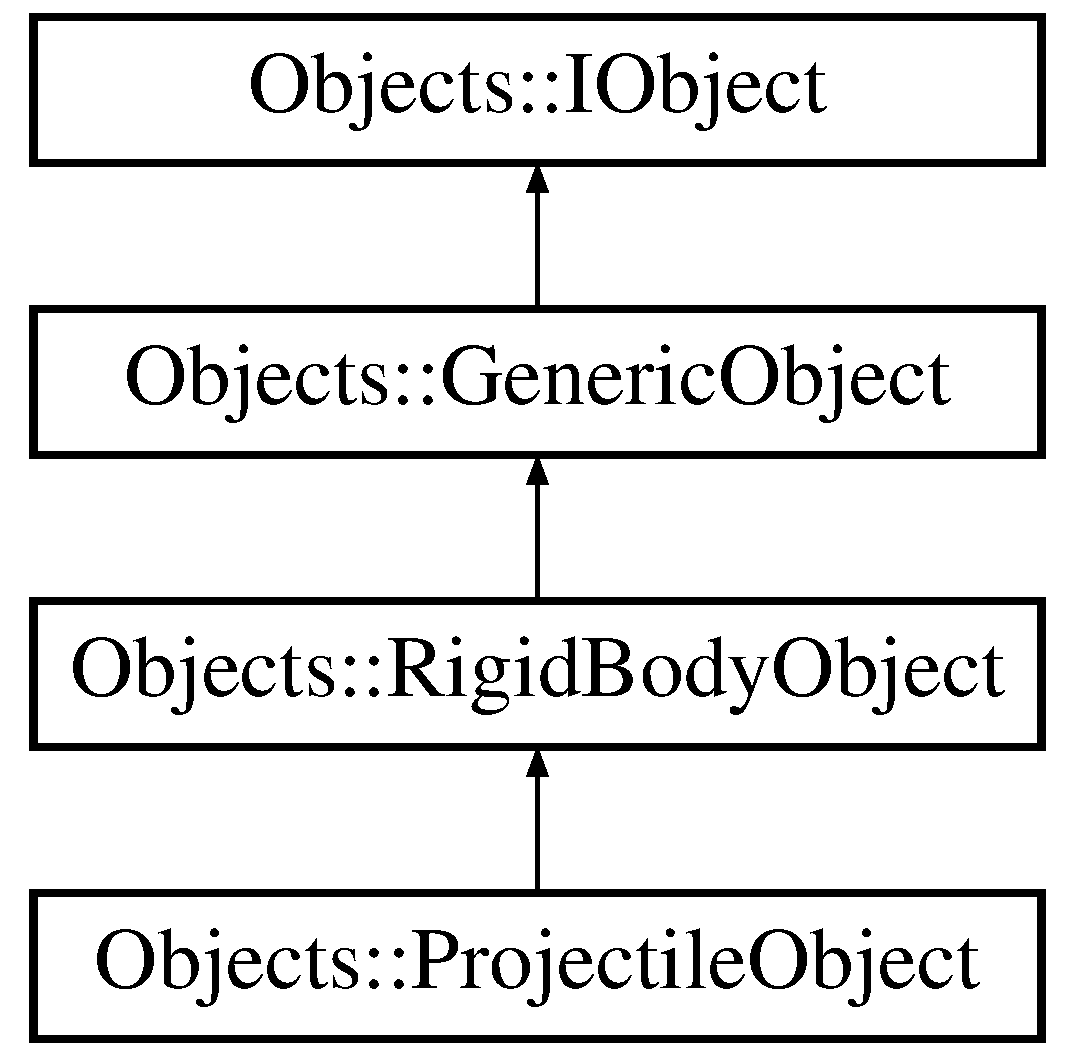
\includegraphics[height=4.000000cm]{class_objects_1_1_projectile_object}
\end{center}
\end{figure}
\subsection*{Public Member Functions}
\begin{DoxyCompactItemize}
\item 
\hypertarget{class_objects_1_1_projectile_object_aa92f0b199905a0a580788764cddf4216}{{\bfseries Projectile\-Object} (Ogre\-::\-Vector3 pos)}\label{class_objects_1_1_projectile_object_aa92f0b199905a0a580788764cddf4216}

\item 
\hypertarget{class_objects_1_1_projectile_object_a8d8fe24f249a79da5970a3daa2cbdf9d}{virtual void \hyperlink{class_objects_1_1_projectile_object_a8d8fe24f249a79da5970a3daa2cbdf9d}{initialise} ()}\label{class_objects_1_1_projectile_object_a8d8fe24f249a79da5970a3daa2cbdf9d}

\begin{DoxyCompactList}\small\item\em Initialises this object. \end{DoxyCompactList}\item 
virtual void \hyperlink{class_objects_1_1_projectile_object_ae8cb3b7f7a9f5b921b043a58e9e355dc}{update} (float delta\-Time)
\begin{DoxyCompactList}\small\item\em Updates the given delta\-Time. \end{DoxyCompactList}\end{DoxyCompactItemize}
\subsection*{Additional Inherited Members}


\subsection{Member Function Documentation}
\hypertarget{class_objects_1_1_projectile_object_ae8cb3b7f7a9f5b921b043a58e9e355dc}{\index{Objects\-::\-Projectile\-Object@{Objects\-::\-Projectile\-Object}!update@{update}}
\index{update@{update}!Objects::ProjectileObject@{Objects\-::\-Projectile\-Object}}
\subsubsection[{update}]{\setlength{\rightskip}{0pt plus 5cm}void Projectile\-Object\-::update (
\begin{DoxyParamCaption}
\item[{float}]{delta\-Time}
\end{DoxyParamCaption}
)\hspace{0.3cm}{\ttfamily [virtual]}}}\label{class_objects_1_1_projectile_object_ae8cb3b7f7a9f5b921b043a58e9e355dc}


Updates the given delta\-Time. 


\begin{DoxyParams}{Parameters}
{\em delta\-Time} & Time of the delta. \\
\hline
\end{DoxyParams}


Reimplemented from \hyperlink{class_objects_1_1_rigid_body_object_a478edcbc5820722a9641fdcd07b402bb}{Objects\-::\-Rigid\-Body\-Object}.



The documentation for this class was generated from the following files\-:\begin{DoxyCompactItemize}
\item 
A\-:/\-I\-T/\-Git\-Hub/\-I\-C\-T312/source/ogregraphics/Projectile\-Object.\-h\item 
A\-:/\-I\-T/\-Git\-Hub/\-I\-C\-T312/source/ogregraphics/Projectile\-Object.\-cpp\end{DoxyCompactItemize}

\hypertarget{class_relax}{\section{Relax Class Reference}
\label{class_relax}\index{Relax@{Relax}}
}


\hyperlink{class_relax}{Relax}.  




{\ttfamily \#include $<$Relax.\-h$>$}

Inheritance diagram for Relax\-:\begin{figure}[H]
\begin{center}
\leavevmode
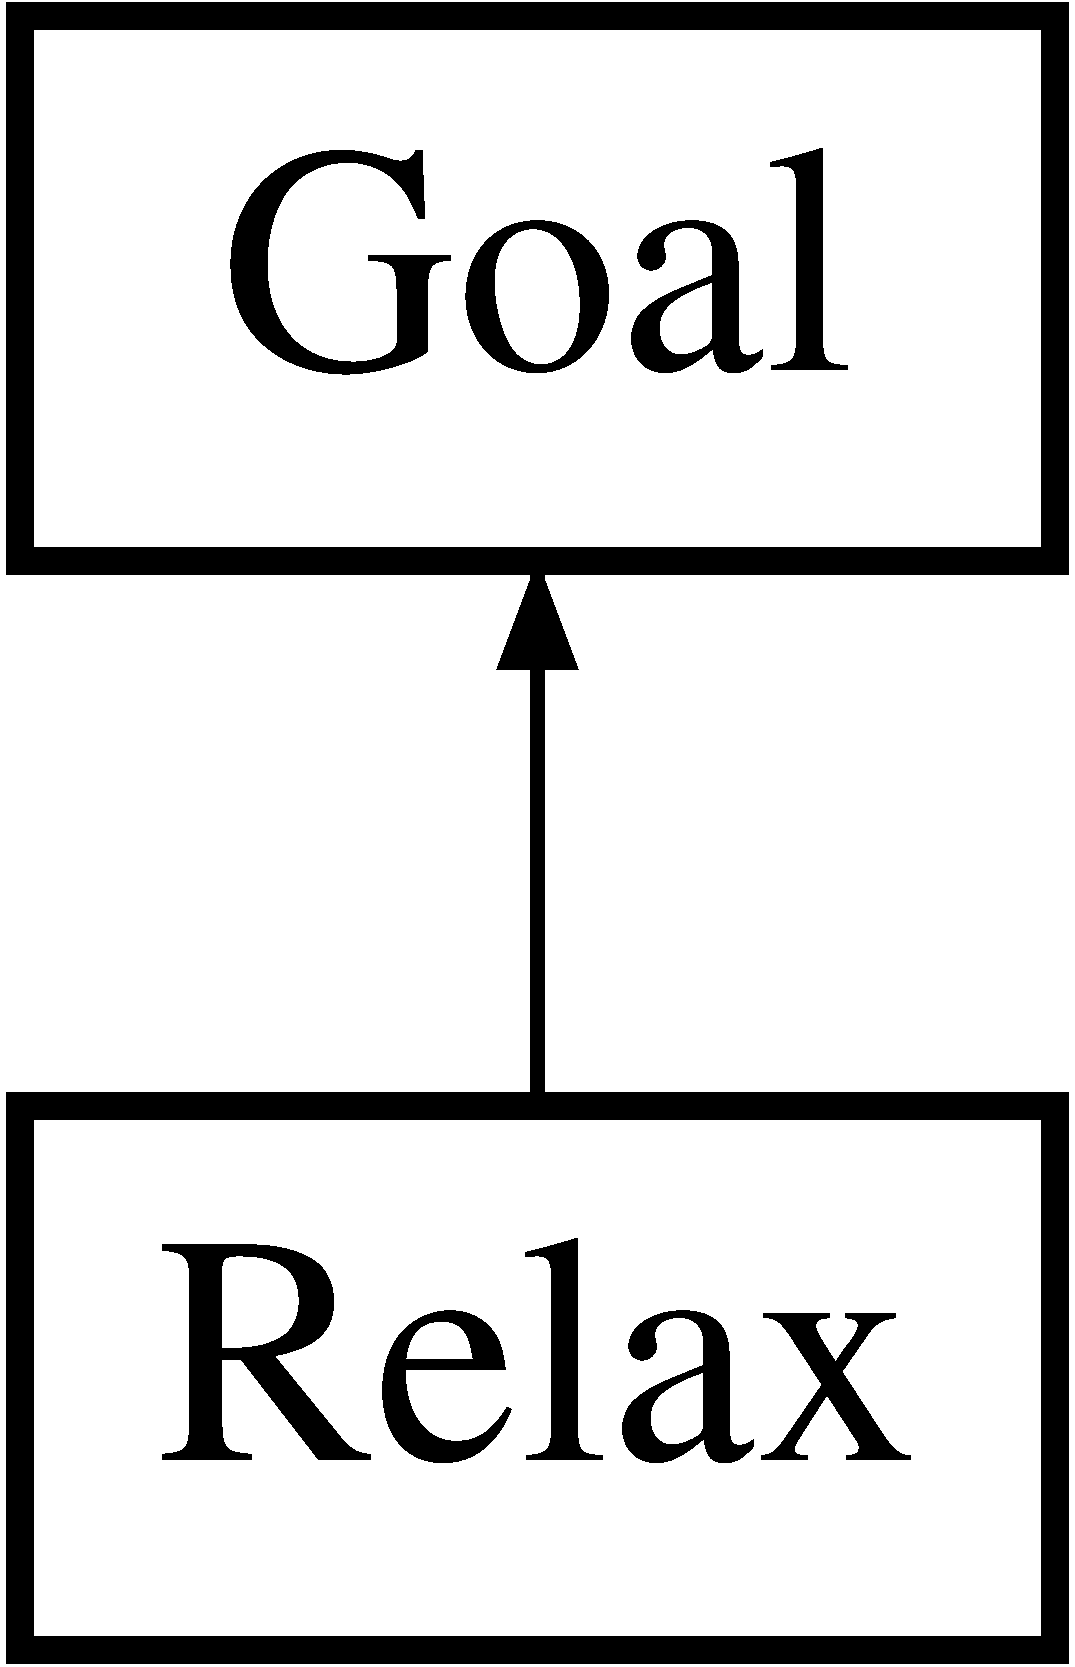
\includegraphics[height=2.000000cm]{class_relax}
\end{center}
\end{figure}
\subsection*{Public Member Functions}
\begin{DoxyCompactItemize}
\item 
\hyperlink{class_relax_a0f1d94211260f96ea86af71412ab36d9}{Relax} (void)
\begin{DoxyCompactList}\small\item\em Default constructor. \end{DoxyCompactList}\item 
\hyperlink{class_relax_a77234cd44af336562af9823f5a3331b6}{$\sim$\-Relax} (void)
\begin{DoxyCompactList}\small\item\em Destructor. \end{DoxyCompactList}\item 
bool \hyperlink{class_relax_acb68b24772650ec9c944e70161f5795f}{Check\-For\-Trigger} (std\-::map$<$ Enum\-Space\-::\-Need\-Types, int $>$)
\begin{DoxyCompactList}\small\item\em Check for trigger. \end{DoxyCompactList}\item 
std\-::map$<$ Enum\-Space\-::\-Need\-Types, \\*
int $>$ $\ast$ \hyperlink{class_relax_a13ab3bd20dc62c0511a657879827feae}{Modify\-Needs} ()
\begin{DoxyCompactList}\small\item\em Gets the modify needs. \end{DoxyCompactList}\end{DoxyCompactItemize}


\subsection{Detailed Description}
\hyperlink{class_relax}{Relax}. 

\begin{DoxyAuthor}{Author}
Hamish Carrier 
\end{DoxyAuthor}
\begin{DoxyDate}{Date}
10/11/2013 
\end{DoxyDate}


\subsection{Constructor \& Destructor Documentation}
\hypertarget{class_relax_a0f1d94211260f96ea86af71412ab36d9}{\index{Relax@{Relax}!Relax@{Relax}}
\index{Relax@{Relax}!Relax@{Relax}}
\subsubsection[{Relax}]{\setlength{\rightskip}{0pt plus 5cm}Relax\-::\-Relax (
\begin{DoxyParamCaption}
\item[{void}]{}
\end{DoxyParamCaption}
)}}\label{class_relax_a0f1d94211260f96ea86af71412ab36d9}


Default constructor. 

\begin{DoxyAuthor}{Author}
Hamish Carrier 
\end{DoxyAuthor}
\begin{DoxyDate}{Date}
10/11/2013 
\end{DoxyDate}
\hypertarget{class_relax_a77234cd44af336562af9823f5a3331b6}{\index{Relax@{Relax}!$\sim$\-Relax@{$\sim$\-Relax}}
\index{$\sim$\-Relax@{$\sim$\-Relax}!Relax@{Relax}}
\subsubsection[{$\sim$\-Relax}]{\setlength{\rightskip}{0pt plus 5cm}Relax\-::$\sim$\-Relax (
\begin{DoxyParamCaption}
\item[{void}]{}
\end{DoxyParamCaption}
)}}\label{class_relax_a77234cd44af336562af9823f5a3331b6}


Destructor. 

\begin{DoxyAuthor}{Author}
Hamish Carrier 
\end{DoxyAuthor}
\begin{DoxyDate}{Date}
10/11/2013 
\end{DoxyDate}


\subsection{Member Function Documentation}
\hypertarget{class_relax_acb68b24772650ec9c944e70161f5795f}{\index{Relax@{Relax}!Check\-For\-Trigger@{Check\-For\-Trigger}}
\index{Check\-For\-Trigger@{Check\-For\-Trigger}!Relax@{Relax}}
\subsubsection[{Check\-For\-Trigger}]{\setlength{\rightskip}{0pt plus 5cm}bool Relax\-::\-Check\-For\-Trigger (
\begin{DoxyParamCaption}
\item[{std\-::map$<$ Enum\-Space\-::\-Need\-Types, int $>$}]{}
\end{DoxyParamCaption}
)}}\label{class_relax_acb68b24772650ec9c944e70161f5795f}


Check for trigger. 

\begin{DoxyAuthor}{Author}
Hamish Carrier 
\end{DoxyAuthor}
\begin{DoxyDate}{Date}
10/11/2013
\end{DoxyDate}

\begin{DoxyParams}{Parameters}
{\em parameter1} & The first parameter.\\
\hline
\end{DoxyParams}
\begin{DoxyReturn}{Returns}
true if it succeeds, false if it fails. 
\end{DoxyReturn}
\hypertarget{class_relax_a13ab3bd20dc62c0511a657879827feae}{\index{Relax@{Relax}!Modify\-Needs@{Modify\-Needs}}
\index{Modify\-Needs@{Modify\-Needs}!Relax@{Relax}}
\subsubsection[{Modify\-Needs}]{\setlength{\rightskip}{0pt plus 5cm}std\-::map$<$ Enum\-Space\-::\-Need\-Types, int $>$ $\ast$ Relax\-::\-Modify\-Needs (
\begin{DoxyParamCaption}
{}
\end{DoxyParamCaption}
)}}\label{class_relax_a13ab3bd20dc62c0511a657879827feae}


Gets the modify needs. 

\begin{DoxyAuthor}{Author}
Hamish Carrier 
\end{DoxyAuthor}
\begin{DoxyDate}{Date}
10/11/2013
\end{DoxyDate}
\begin{DoxyReturn}{Returns}
null if it fails, else. 
\end{DoxyReturn}


The documentation for this class was generated from the following files\-:\begin{DoxyCompactItemize}
\item 
A\-:/\-I\-T/\-Git\-Hub/\-I\-C\-T312/source/ogregraphics/\hyperlink{_relax_8h}{Relax.\-h}\item 
A\-:/\-I\-T/\-Git\-Hub/\-I\-C\-T312/source/ogregraphics/Relax.\-cpp\end{DoxyCompactItemize}

\hypertarget{class_objects_1_1_rigid_body_object}{\section{Objects\-:\-:Rigid\-Body\-Object Class Reference}
\label{class_objects_1_1_rigid_body_object}\index{Objects\-::\-Rigid\-Body\-Object@{Objects\-::\-Rigid\-Body\-Object}}
}


Rigid body object.  




{\ttfamily \#include $<$Rigid\-Body\-Object.\-h$>$}

Inheritance diagram for Objects\-:\-:Rigid\-Body\-Object\-:\begin{figure}[H]
\begin{center}
\leavevmode
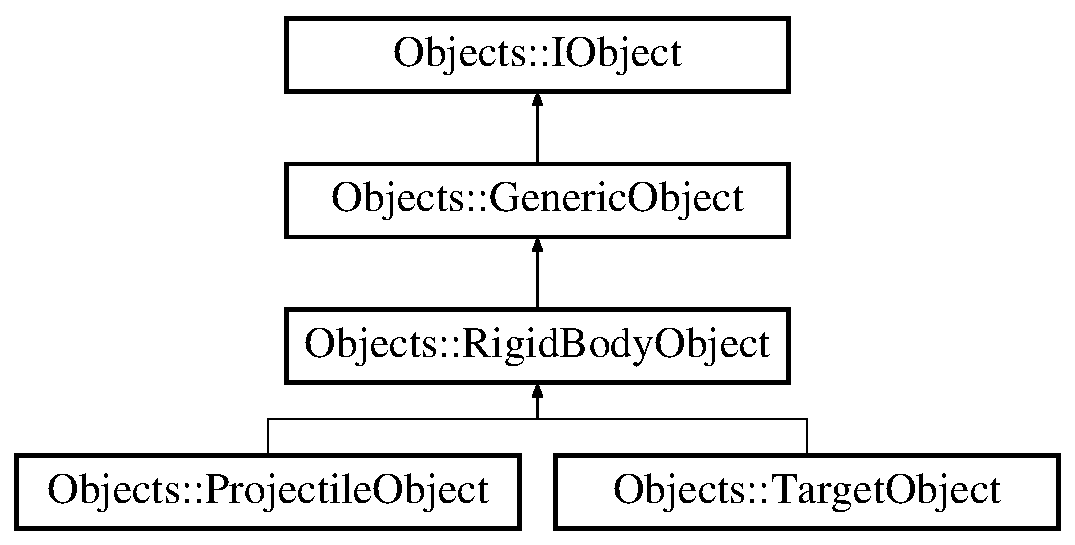
\includegraphics[height=4.000000cm]{class_objects_1_1_rigid_body_object}
\end{center}
\end{figure}
\subsection*{Public Member Functions}
\begin{DoxyCompactItemize}
\item 
\hyperlink{class_objects_1_1_rigid_body_object_a1ed19d8ed67672ed4a7b1c824c95f592}{Rigid\-Body\-Object} (std\-::string mesh\-File)
\begin{DoxyCompactList}\small\item\em Constructor. \end{DoxyCompactList}\item 
\hyperlink{class_objects_1_1_rigid_body_object_aaa91269d5e4e1c25d8f2f4dd1edc1dee}{Rigid\-Body\-Object} (Ogre\-::\-Vector3 pos, Ogre\-::\-Quaternion rot, Ogre\-::\-Vector3 scale, std\-::string mesh\-File)
\begin{DoxyCompactList}\small\item\em Constructor. \end{DoxyCompactList}\item 
\hypertarget{class_objects_1_1_rigid_body_object_abd8cfa1d049fcdffd725118f29e8d4d0}{\hyperlink{class_objects_1_1_rigid_body_object_abd8cfa1d049fcdffd725118f29e8d4d0}{$\sim$\-Rigid\-Body\-Object} (void)}\label{class_objects_1_1_rigid_body_object_abd8cfa1d049fcdffd725118f29e8d4d0}

\begin{DoxyCompactList}\small\item\em Destructor. \end{DoxyCompactList}\item 
\hypertarget{class_objects_1_1_rigid_body_object_a08f19a117e240c6234350b0f9404fbc9}{virtual void \hyperlink{class_objects_1_1_rigid_body_object_a08f19a117e240c6234350b0f9404fbc9}{initialise} ()}\label{class_objects_1_1_rigid_body_object_a08f19a117e240c6234350b0f9404fbc9}

\begin{DoxyCompactList}\small\item\em Initialises this object. \end{DoxyCompactList}\item 
virtual void \hyperlink{class_objects_1_1_rigid_body_object_a478edcbc5820722a9641fdcd07b402bb}{update} (float delta\-Time)
\begin{DoxyCompactList}\small\item\em Updates the given delta\-Time. \end{DoxyCompactList}\item 
void \hyperlink{class_objects_1_1_rigid_body_object_a4962caad85c4a7c19039ca937079daa1}{set\-Angular\-Velocity} (Ogre\-::\-Vector3 axis, float angle)
\begin{DoxyCompactList}\small\item\em Sets angular velocity. \end{DoxyCompactList}\item 
void \hyperlink{class_objects_1_1_rigid_body_object_a721c1dc9a881fab6db36f60edb715fbd}{apply\-Force} (Ogre\-::\-Vector3 force)
\begin{DoxyCompactList}\small\item\em Applies the force described by force. \end{DoxyCompactList}\item 
void \hyperlink{class_objects_1_1_rigid_body_object_afae0c2363af38e3c691d37204a489505}{set\-Velocity} (Ogre\-::\-Vector3 vel)
\begin{DoxyCompactList}\small\item\em void apply\-Force(\-Physics\-::\-Force force); \end{DoxyCompactList}\item 
Ogre\-::\-Vector3 \hyperlink{class_objects_1_1_rigid_body_object_a722575b42384d8d7be5f123ae8ecc21c}{get\-Velocity} ()
\begin{DoxyCompactList}\small\item\em Gets the velocity. \end{DoxyCompactList}\item 
Ogre\-::\-Vector3 \hyperlink{class_objects_1_1_rigid_body_object_ac6056bc9cf0fa789e46c66bbc3c465c3}{get\-Last\-Acceleration} ()
\begin{DoxyCompactList}\small\item\em Gets the last acceleration. \end{DoxyCompactList}\item 
float \hyperlink{class_objects_1_1_rigid_body_object_a9195f7e6e5854c894e1b0e4643f39340}{get\-Mass} ()
\begin{DoxyCompactList}\small\item\em Gets the mass. \end{DoxyCompactList}\item 
void \hyperlink{class_objects_1_1_rigid_body_object_a05acd53aaf329569d1454eb12ad7e282}{set\-Mass} (float mass)
\begin{DoxyCompactList}\small\item\em Sets the mass. \end{DoxyCompactList}\item 
float \hyperlink{class_objects_1_1_rigid_body_object_a1b037499bc2350cb6f453c22cfb6866a}{get\-Inverse\-Mass} ()
\begin{DoxyCompactList}\small\item\em Gets inverse mass. \end{DoxyCompactList}\item 
void \hyperlink{class_objects_1_1_rigid_body_object_a07cbd5667c70936f0384fd29bd87f6cc}{add\-Velocity} (Ogre\-::\-Vector3 \&velocity)
\begin{DoxyCompactList}\small\item\em Adds a velocity. \end{DoxyCompactList}\item 
void \hyperlink{class_objects_1_1_rigid_body_object_aae35d039b1fc774135427918ac97b85b}{add\-Rotation} (Ogre\-::\-Vector3 \&rotation)
\begin{DoxyCompactList}\small\item\em Adds a rotation. \end{DoxyCompactList}\item 
Ogre\-::\-Matrix3 \hyperlink{class_objects_1_1_rigid_body_object_aa9834cc73862604017850623250fb66a}{get\-Inverse\-Inertia\-Tensor\-World} ()
\begin{DoxyCompactList}\small\item\em Gets inverse inertia tensor world. \end{DoxyCompactList}\item 
void \hyperlink{class_objects_1_1_rigid_body_object_a4b0ffccc0f8a9915f16baaf92c39bf25}{set\-Inertia\-Tensor} (Ogre\-::\-Matrix3 tensor)
\begin{DoxyCompactList}\small\item\em Sets inertia tensor. \end{DoxyCompactList}\end{DoxyCompactItemize}
\subsection*{Static Public Member Functions}
\begin{DoxyCompactItemize}
\item 
static Ogre\-::\-Matrix3 \hyperlink{class_objects_1_1_rigid_body_object_aa2d2a29fce3f2f6e893bf16cd965cc45}{Inertia\-Tensor\-Solid\-Sphere} (float radius, float mass)
\begin{DoxyCompactList}\small\item\em Inertia tensor solid sphere. \end{DoxyCompactList}\item 
static Ogre\-::\-Matrix3 \hyperlink{class_objects_1_1_rigid_body_object_a5b7c2c8986ef85a532c149b6a2364c83}{Inertia\-Tensor\-Sphere\-Shell} (float radius, float mass)
\begin{DoxyCompactList}\small\item\em Inertia tensor sphere shell. \end{DoxyCompactList}\item 
static Ogre\-::\-Matrix3 \hyperlink{class_objects_1_1_rigid_body_object_ad18e3a54eb181c68c17699969580bef1}{Inertia\-Tensor\-Cuboid} (float width, float height, float depth, float mass)
\begin{DoxyCompactList}\small\item\em width in x, height in y, depth in z. \end{DoxyCompactList}\item 
static Ogre\-::\-Matrix3 \hyperlink{class_objects_1_1_rigid_body_object_a94345e8ddfed29826c8b53d4aff2ee7a}{Inertia\-Tensor\-Solid\-Cylinder} (float radius, float height, float mass)
\begin{DoxyCompactList}\small\item\em Inertia tensor solid cylinder. \end{DoxyCompactList}\item 
static void \hyperlink{class_objects_1_1_rigid_body_object_af2cc1454d37839b75ad66afd8a70b926}{calculate\-Transform\-Matrix} (Ogre\-::\-Matrix4 \&transform, const Ogre\-::\-Vector3 \&pos, const Ogre\-::\-Quaternion \&orientation)
\begin{DoxyCompactList}\small\item\em Calculates the transform matrix. \end{DoxyCompactList}\item 
static void \hyperlink{class_objects_1_1_rigid_body_object_ac64b21afafd915bb3c8bfc6311920b67}{transform\-Inertia\-Tensor} (Ogre\-::\-Matrix3 \&iit\-World, const Ogre\-::\-Quaternion \&quat, const Ogre\-::\-Matrix3 \&iit\-Body, const Ogre\-::\-Matrix4 \&trans\-Mat)
\begin{DoxyCompactList}\small\item\em Transform inertia tensor. \end{DoxyCompactList}\end{DoxyCompactItemize}
\subsection*{Protected Attributes}
\begin{DoxyCompactItemize}
\item 
\hypertarget{class_objects_1_1_rigid_body_object_a957bd48ab183589d92a4994086fde8da}{Ogre\-::\-Vector3 \hyperlink{class_objects_1_1_rigid_body_object_a957bd48ab183589d92a4994086fde8da}{m\-\_\-force}}\label{class_objects_1_1_rigid_body_object_a957bd48ab183589d92a4994086fde8da}

\begin{DoxyCompactList}\small\item\em The force. \end{DoxyCompactList}\item 
\hypertarget{class_objects_1_1_rigid_body_object_a7cbfd216782247323829a9f88874fcc8}{float \hyperlink{class_objects_1_1_rigid_body_object_a7cbfd216782247323829a9f88874fcc8}{m\-\_\-mass}}\label{class_objects_1_1_rigid_body_object_a7cbfd216782247323829a9f88874fcc8}

\begin{DoxyCompactList}\small\item\em The mass. \end{DoxyCompactList}\item 
\hypertarget{class_objects_1_1_rigid_body_object_ab66659e28108e20af4f1d5c5b660a69e}{float \hyperlink{class_objects_1_1_rigid_body_object_ab66659e28108e20af4f1d5c5b660a69e}{m\-\_\-inv\-Mass}}\label{class_objects_1_1_rigid_body_object_ab66659e28108e20af4f1d5c5b660a69e}

\begin{DoxyCompactList}\small\item\em The inverse mass. \end{DoxyCompactList}\item 
\hypertarget{class_objects_1_1_rigid_body_object_abb70e651df485861e6f021733b5d6170}{Ogre\-::\-Matrix3 \hyperlink{class_objects_1_1_rigid_body_object_abb70e651df485861e6f021733b5d6170}{m\-\_\-inertia\-Tensor}}\label{class_objects_1_1_rigid_body_object_abb70e651df485861e6f021733b5d6170}

\begin{DoxyCompactList}\small\item\em The inertia tensor. \end{DoxyCompactList}\item 
\hypertarget{class_objects_1_1_rigid_body_object_a4b159406f8cfda0f828fd3c71f94d3b4}{Ogre\-::\-Matrix3 \hyperlink{class_objects_1_1_rigid_body_object_a4b159406f8cfda0f828fd3c71f94d3b4}{m\-\_\-inv\-Inertia\-Tensor}}\label{class_objects_1_1_rigid_body_object_a4b159406f8cfda0f828fd3c71f94d3b4}

\begin{DoxyCompactList}\small\item\em The inverse inertia tensor. \end{DoxyCompactList}\item 
\hypertarget{class_objects_1_1_rigid_body_object_aee45c14355de99ed03029cdd7ba22afb}{Ogre\-::\-Matrix3 \hyperlink{class_objects_1_1_rigid_body_object_aee45c14355de99ed03029cdd7ba22afb}{m\-\_\-inv\-Inertia\-Tensor\-World}}\label{class_objects_1_1_rigid_body_object_aee45c14355de99ed03029cdd7ba22afb}

\begin{DoxyCompactList}\small\item\em The inverse inertia tensor world. \end{DoxyCompactList}\item 
\hypertarget{class_objects_1_1_rigid_body_object_a9c0000fd5877b44539edd45b8a5429f8}{Ogre\-::\-Matrix4 \hyperlink{class_objects_1_1_rigid_body_object_a9c0000fd5877b44539edd45b8a5429f8}{m\-\_\-transform\-Matrix}}\label{class_objects_1_1_rigid_body_object_a9c0000fd5877b44539edd45b8a5429f8}

\begin{DoxyCompactList}\small\item\em The transform matrix. \end{DoxyCompactList}\item 
\hypertarget{class_objects_1_1_rigid_body_object_a79df3f4621fd7ce78ae866a4ee426d2b}{Ogre\-::\-Vector3 \hyperlink{class_objects_1_1_rigid_body_object_a79df3f4621fd7ce78ae866a4ee426d2b}{m\-\_\-angular\-Velocity}}\label{class_objects_1_1_rigid_body_object_a79df3f4621fd7ce78ae866a4ee426d2b}

\begin{DoxyCompactList}\small\item\em The angular velocity. \end{DoxyCompactList}\item 
\hypertarget{class_objects_1_1_rigid_body_object_aa5ee455d9e5ae6a879795ecb89c61bf8}{Ogre\-::\-Vector3 \hyperlink{class_objects_1_1_rigid_body_object_aa5ee455d9e5ae6a879795ecb89c61bf8}{m\-\_\-acceleration}}\label{class_objects_1_1_rigid_body_object_aa5ee455d9e5ae6a879795ecb89c61bf8}

\begin{DoxyCompactList}\small\item\em The acceleration. \end{DoxyCompactList}\item 
\hypertarget{class_objects_1_1_rigid_body_object_a33d8217f62d2e76558f5c22c4c33391e}{Ogre\-::\-Vector3 \hyperlink{class_objects_1_1_rigid_body_object_a33d8217f62d2e76558f5c22c4c33391e}{m\-\_\-velocity}}\label{class_objects_1_1_rigid_body_object_a33d8217f62d2e76558f5c22c4c33391e}

\begin{DoxyCompactList}\small\item\em The velocity. \end{DoxyCompactList}\item 
\hypertarget{class_objects_1_1_rigid_body_object_ae8a1fdc0cb614d6fb71dcfffd3e8741a}{Ogre\-::\-Vector3 \hyperlink{class_objects_1_1_rigid_body_object_ae8a1fdc0cb614d6fb71dcfffd3e8741a}{m\-\_\-last\-Acceleration}}\label{class_objects_1_1_rigid_body_object_ae8a1fdc0cb614d6fb71dcfffd3e8741a}

\begin{DoxyCompactList}\small\item\em The last acceleration. \end{DoxyCompactList}\end{DoxyCompactItemize}
\subsection*{Additional Inherited Members}


\subsection{Detailed Description}
Rigid body object. 

\subsection{Constructor \& Destructor Documentation}
\hypertarget{class_objects_1_1_rigid_body_object_a1ed19d8ed67672ed4a7b1c824c95f592}{\index{Objects\-::\-Rigid\-Body\-Object@{Objects\-::\-Rigid\-Body\-Object}!Rigid\-Body\-Object@{Rigid\-Body\-Object}}
\index{Rigid\-Body\-Object@{Rigid\-Body\-Object}!Objects::RigidBodyObject@{Objects\-::\-Rigid\-Body\-Object}}
\subsubsection[{Rigid\-Body\-Object}]{\setlength{\rightskip}{0pt plus 5cm}Objects\-::\-Rigid\-Body\-Object\-::\-Rigid\-Body\-Object (
\begin{DoxyParamCaption}
\item[{std\-::string}]{mesh\-File}
\end{DoxyParamCaption}
)}}\label{class_objects_1_1_rigid_body_object_a1ed19d8ed67672ed4a7b1c824c95f592}


Constructor. 


\begin{DoxyParams}{Parameters}
{\em mesh\-File} & The mesh file. \\
\hline
\end{DoxyParams}
\hypertarget{class_objects_1_1_rigid_body_object_aaa91269d5e4e1c25d8f2f4dd1edc1dee}{\index{Objects\-::\-Rigid\-Body\-Object@{Objects\-::\-Rigid\-Body\-Object}!Rigid\-Body\-Object@{Rigid\-Body\-Object}}
\index{Rigid\-Body\-Object@{Rigid\-Body\-Object}!Objects::RigidBodyObject@{Objects\-::\-Rigid\-Body\-Object}}
\subsubsection[{Rigid\-Body\-Object}]{\setlength{\rightskip}{0pt plus 5cm}Objects\-::\-Rigid\-Body\-Object\-::\-Rigid\-Body\-Object (
\begin{DoxyParamCaption}
\item[{Ogre\-::\-Vector3}]{pos, }
\item[{Ogre\-::\-Quaternion}]{rot, }
\item[{Ogre\-::\-Vector3}]{scale, }
\item[{std\-::string}]{mesh\-File}
\end{DoxyParamCaption}
)}}\label{class_objects_1_1_rigid_body_object_aaa91269d5e4e1c25d8f2f4dd1edc1dee}


Constructor. 


\begin{DoxyParams}{Parameters}
{\em pos} & The position. \\
\hline
{\em rot} & The rot. \\
\hline
{\em scale} & The scale. \\
\hline
{\em mesh\-File} & The mesh file. \\
\hline
\end{DoxyParams}


\subsection{Member Function Documentation}
\hypertarget{class_objects_1_1_rigid_body_object_aae35d039b1fc774135427918ac97b85b}{\index{Objects\-::\-Rigid\-Body\-Object@{Objects\-::\-Rigid\-Body\-Object}!add\-Rotation@{add\-Rotation}}
\index{add\-Rotation@{add\-Rotation}!Objects::RigidBodyObject@{Objects\-::\-Rigid\-Body\-Object}}
\subsubsection[{add\-Rotation}]{\setlength{\rightskip}{0pt plus 5cm}void Objects\-::\-Rigid\-Body\-Object\-::add\-Rotation (
\begin{DoxyParamCaption}
\item[{Ogre\-::\-Vector3 \&}]{rotation}
\end{DoxyParamCaption}
)}}\label{class_objects_1_1_rigid_body_object_aae35d039b1fc774135427918ac97b85b}


Adds a rotation. 


\begin{DoxyParams}[1]{Parameters}
\mbox{\tt in,out}  & {\em rotation} & The rotation. \\
\hline
\end{DoxyParams}
\hypertarget{class_objects_1_1_rigid_body_object_a07cbd5667c70936f0384fd29bd87f6cc}{\index{Objects\-::\-Rigid\-Body\-Object@{Objects\-::\-Rigid\-Body\-Object}!add\-Velocity@{add\-Velocity}}
\index{add\-Velocity@{add\-Velocity}!Objects::RigidBodyObject@{Objects\-::\-Rigid\-Body\-Object}}
\subsubsection[{add\-Velocity}]{\setlength{\rightskip}{0pt plus 5cm}void Objects\-::\-Rigid\-Body\-Object\-::add\-Velocity (
\begin{DoxyParamCaption}
\item[{Ogre\-::\-Vector3 \&}]{velocity}
\end{DoxyParamCaption}
)}}\label{class_objects_1_1_rigid_body_object_a07cbd5667c70936f0384fd29bd87f6cc}


Adds a velocity. 


\begin{DoxyParams}[1]{Parameters}
\mbox{\tt in,out}  & {\em velocity} & The velocity. \\
\hline
\end{DoxyParams}
\hypertarget{class_objects_1_1_rigid_body_object_a721c1dc9a881fab6db36f60edb715fbd}{\index{Objects\-::\-Rigid\-Body\-Object@{Objects\-::\-Rigid\-Body\-Object}!apply\-Force@{apply\-Force}}
\index{apply\-Force@{apply\-Force}!Objects::RigidBodyObject@{Objects\-::\-Rigid\-Body\-Object}}
\subsubsection[{apply\-Force}]{\setlength{\rightskip}{0pt plus 5cm}void Objects\-::\-Rigid\-Body\-Object\-::apply\-Force (
\begin{DoxyParamCaption}
\item[{Ogre\-::\-Vector3}]{force}
\end{DoxyParamCaption}
)}}\label{class_objects_1_1_rigid_body_object_a721c1dc9a881fab6db36f60edb715fbd}


Applies the force described by force. 


\begin{DoxyParams}{Parameters}
{\em force} & The force. \\
\hline
\end{DoxyParams}
\hypertarget{class_objects_1_1_rigid_body_object_af2cc1454d37839b75ad66afd8a70b926}{\index{Objects\-::\-Rigid\-Body\-Object@{Objects\-::\-Rigid\-Body\-Object}!calculate\-Transform\-Matrix@{calculate\-Transform\-Matrix}}
\index{calculate\-Transform\-Matrix@{calculate\-Transform\-Matrix}!Objects::RigidBodyObject@{Objects\-::\-Rigid\-Body\-Object}}
\subsubsection[{calculate\-Transform\-Matrix}]{\setlength{\rightskip}{0pt plus 5cm}static void Objects\-::\-Rigid\-Body\-Object\-::calculate\-Transform\-Matrix (
\begin{DoxyParamCaption}
\item[{Ogre\-::\-Matrix4 \&}]{transform, }
\item[{const Ogre\-::\-Vector3 \&}]{pos, }
\item[{const Ogre\-::\-Quaternion \&}]{orientation}
\end{DoxyParamCaption}
)\hspace{0.3cm}{\ttfamily [static]}}}\label{class_objects_1_1_rigid_body_object_af2cc1454d37839b75ad66afd8a70b926}


Calculates the transform matrix. 


\begin{DoxyParams}[1]{Parameters}
\mbox{\tt in,out}  & {\em transform} & The transform. \\
\hline
 & {\em pos} & The position. \\
\hline
 & {\em orientation} & The orientation. \\
\hline
\end{DoxyParams}
\hypertarget{class_objects_1_1_rigid_body_object_aa9834cc73862604017850623250fb66a}{\index{Objects\-::\-Rigid\-Body\-Object@{Objects\-::\-Rigid\-Body\-Object}!get\-Inverse\-Inertia\-Tensor\-World@{get\-Inverse\-Inertia\-Tensor\-World}}
\index{get\-Inverse\-Inertia\-Tensor\-World@{get\-Inverse\-Inertia\-Tensor\-World}!Objects::RigidBodyObject@{Objects\-::\-Rigid\-Body\-Object}}
\subsubsection[{get\-Inverse\-Inertia\-Tensor\-World}]{\setlength{\rightskip}{0pt plus 5cm}Ogre\-::\-Matrix3 Objects\-::\-Rigid\-Body\-Object\-::get\-Inverse\-Inertia\-Tensor\-World (
\begin{DoxyParamCaption}
{}
\end{DoxyParamCaption}
)\hspace{0.3cm}{\ttfamily [inline]}}}\label{class_objects_1_1_rigid_body_object_aa9834cc73862604017850623250fb66a}


Gets inverse inertia tensor world. 

\begin{DoxyReturn}{Returns}
The inverse inertia tensor world. 
\end{DoxyReturn}
\hypertarget{class_objects_1_1_rigid_body_object_a1b037499bc2350cb6f453c22cfb6866a}{\index{Objects\-::\-Rigid\-Body\-Object@{Objects\-::\-Rigid\-Body\-Object}!get\-Inverse\-Mass@{get\-Inverse\-Mass}}
\index{get\-Inverse\-Mass@{get\-Inverse\-Mass}!Objects::RigidBodyObject@{Objects\-::\-Rigid\-Body\-Object}}
\subsubsection[{get\-Inverse\-Mass}]{\setlength{\rightskip}{0pt plus 5cm}float Objects\-::\-Rigid\-Body\-Object\-::get\-Inverse\-Mass (
\begin{DoxyParamCaption}
{}
\end{DoxyParamCaption}
)\hspace{0.3cm}{\ttfamily [inline]}}}\label{class_objects_1_1_rigid_body_object_a1b037499bc2350cb6f453c22cfb6866a}


Gets inverse mass. 

\begin{DoxyReturn}{Returns}
The inverse mass. 
\end{DoxyReturn}
\hypertarget{class_objects_1_1_rigid_body_object_ac6056bc9cf0fa789e46c66bbc3c465c3}{\index{Objects\-::\-Rigid\-Body\-Object@{Objects\-::\-Rigid\-Body\-Object}!get\-Last\-Acceleration@{get\-Last\-Acceleration}}
\index{get\-Last\-Acceleration@{get\-Last\-Acceleration}!Objects::RigidBodyObject@{Objects\-::\-Rigid\-Body\-Object}}
\subsubsection[{get\-Last\-Acceleration}]{\setlength{\rightskip}{0pt plus 5cm}Ogre\-::\-Vector3 Objects\-::\-Rigid\-Body\-Object\-::get\-Last\-Acceleration (
\begin{DoxyParamCaption}
{}
\end{DoxyParamCaption}
)\hspace{0.3cm}{\ttfamily [inline]}}}\label{class_objects_1_1_rigid_body_object_ac6056bc9cf0fa789e46c66bbc3c465c3}


Gets the last acceleration. 

\begin{DoxyReturn}{Returns}
The last acceleration. 
\end{DoxyReturn}
\hypertarget{class_objects_1_1_rigid_body_object_a9195f7e6e5854c894e1b0e4643f39340}{\index{Objects\-::\-Rigid\-Body\-Object@{Objects\-::\-Rigid\-Body\-Object}!get\-Mass@{get\-Mass}}
\index{get\-Mass@{get\-Mass}!Objects::RigidBodyObject@{Objects\-::\-Rigid\-Body\-Object}}
\subsubsection[{get\-Mass}]{\setlength{\rightskip}{0pt plus 5cm}float Objects\-::\-Rigid\-Body\-Object\-::get\-Mass (
\begin{DoxyParamCaption}
{}
\end{DoxyParamCaption}
)\hspace{0.3cm}{\ttfamily [inline]}}}\label{class_objects_1_1_rigid_body_object_a9195f7e6e5854c894e1b0e4643f39340}


Gets the mass. 

\begin{DoxyReturn}{Returns}
The mass. 
\end{DoxyReturn}
\hypertarget{class_objects_1_1_rigid_body_object_a722575b42384d8d7be5f123ae8ecc21c}{\index{Objects\-::\-Rigid\-Body\-Object@{Objects\-::\-Rigid\-Body\-Object}!get\-Velocity@{get\-Velocity}}
\index{get\-Velocity@{get\-Velocity}!Objects::RigidBodyObject@{Objects\-::\-Rigid\-Body\-Object}}
\subsubsection[{get\-Velocity}]{\setlength{\rightskip}{0pt plus 5cm}Ogre\-::\-Vector3 Objects\-::\-Rigid\-Body\-Object\-::get\-Velocity (
\begin{DoxyParamCaption}
{}
\end{DoxyParamCaption}
)\hspace{0.3cm}{\ttfamily [inline]}}}\label{class_objects_1_1_rigid_body_object_a722575b42384d8d7be5f123ae8ecc21c}


Gets the velocity. 

\begin{DoxyReturn}{Returns}
The velocity. 
\end{DoxyReturn}
\hypertarget{class_objects_1_1_rigid_body_object_ad18e3a54eb181c68c17699969580bef1}{\index{Objects\-::\-Rigid\-Body\-Object@{Objects\-::\-Rigid\-Body\-Object}!Inertia\-Tensor\-Cuboid@{Inertia\-Tensor\-Cuboid}}
\index{Inertia\-Tensor\-Cuboid@{Inertia\-Tensor\-Cuboid}!Objects::RigidBodyObject@{Objects\-::\-Rigid\-Body\-Object}}
\subsubsection[{Inertia\-Tensor\-Cuboid}]{\setlength{\rightskip}{0pt plus 5cm}static Ogre\-::\-Matrix3 Objects\-::\-Rigid\-Body\-Object\-::\-Inertia\-Tensor\-Cuboid (
\begin{DoxyParamCaption}
\item[{float}]{width, }
\item[{float}]{height, }
\item[{float}]{depth, }
\item[{float}]{mass}
\end{DoxyParamCaption}
)\hspace{0.3cm}{\ttfamily [static]}}}\label{class_objects_1_1_rigid_body_object_ad18e3a54eb181c68c17699969580bef1}


width in x, height in y, depth in z. 


\begin{DoxyParams}{Parameters}
{\em width} & The width. \\
\hline
{\em height} & The height. \\
\hline
{\em depth} & The depth. \\
\hline
{\em mass} & The mass.\\
\hline
\end{DoxyParams}
\begin{DoxyReturn}{Returns}
. 
\end{DoxyReturn}
\hypertarget{class_objects_1_1_rigid_body_object_a94345e8ddfed29826c8b53d4aff2ee7a}{\index{Objects\-::\-Rigid\-Body\-Object@{Objects\-::\-Rigid\-Body\-Object}!Inertia\-Tensor\-Solid\-Cylinder@{Inertia\-Tensor\-Solid\-Cylinder}}
\index{Inertia\-Tensor\-Solid\-Cylinder@{Inertia\-Tensor\-Solid\-Cylinder}!Objects::RigidBodyObject@{Objects\-::\-Rigid\-Body\-Object}}
\subsubsection[{Inertia\-Tensor\-Solid\-Cylinder}]{\setlength{\rightskip}{0pt plus 5cm}static Ogre\-::\-Matrix3 Objects\-::\-Rigid\-Body\-Object\-::\-Inertia\-Tensor\-Solid\-Cylinder (
\begin{DoxyParamCaption}
\item[{float}]{radius, }
\item[{float}]{height, }
\item[{float}]{mass}
\end{DoxyParamCaption}
)\hspace{0.3cm}{\ttfamily [static]}}}\label{class_objects_1_1_rigid_body_object_a94345e8ddfed29826c8b53d4aff2ee7a}


Inertia tensor solid cylinder. 


\begin{DoxyParams}{Parameters}
{\em radius} & The radius. \\
\hline
{\em height} & The height. \\
\hline
{\em mass} & The mass.\\
\hline
\end{DoxyParams}
\begin{DoxyReturn}{Returns}
. 
\end{DoxyReturn}
\hypertarget{class_objects_1_1_rigid_body_object_aa2d2a29fce3f2f6e893bf16cd965cc45}{\index{Objects\-::\-Rigid\-Body\-Object@{Objects\-::\-Rigid\-Body\-Object}!Inertia\-Tensor\-Solid\-Sphere@{Inertia\-Tensor\-Solid\-Sphere}}
\index{Inertia\-Tensor\-Solid\-Sphere@{Inertia\-Tensor\-Solid\-Sphere}!Objects::RigidBodyObject@{Objects\-::\-Rigid\-Body\-Object}}
\subsubsection[{Inertia\-Tensor\-Solid\-Sphere}]{\setlength{\rightskip}{0pt plus 5cm}static Ogre\-::\-Matrix3 Objects\-::\-Rigid\-Body\-Object\-::\-Inertia\-Tensor\-Solid\-Sphere (
\begin{DoxyParamCaption}
\item[{float}]{radius, }
\item[{float}]{mass}
\end{DoxyParamCaption}
)\hspace{0.3cm}{\ttfamily [static]}}}\label{class_objects_1_1_rigid_body_object_aa2d2a29fce3f2f6e893bf16cd965cc45}


Inertia tensor solid sphere. 


\begin{DoxyParams}{Parameters}
{\em radius} & The radius. \\
\hline
{\em mass} & The mass.\\
\hline
\end{DoxyParams}
\begin{DoxyReturn}{Returns}
. 
\end{DoxyReturn}
\hypertarget{class_objects_1_1_rigid_body_object_a5b7c2c8986ef85a532c149b6a2364c83}{\index{Objects\-::\-Rigid\-Body\-Object@{Objects\-::\-Rigid\-Body\-Object}!Inertia\-Tensor\-Sphere\-Shell@{Inertia\-Tensor\-Sphere\-Shell}}
\index{Inertia\-Tensor\-Sphere\-Shell@{Inertia\-Tensor\-Sphere\-Shell}!Objects::RigidBodyObject@{Objects\-::\-Rigid\-Body\-Object}}
\subsubsection[{Inertia\-Tensor\-Sphere\-Shell}]{\setlength{\rightskip}{0pt plus 5cm}static Ogre\-::\-Matrix3 Objects\-::\-Rigid\-Body\-Object\-::\-Inertia\-Tensor\-Sphere\-Shell (
\begin{DoxyParamCaption}
\item[{float}]{radius, }
\item[{float}]{mass}
\end{DoxyParamCaption}
)\hspace{0.3cm}{\ttfamily [static]}}}\label{class_objects_1_1_rigid_body_object_a5b7c2c8986ef85a532c149b6a2364c83}


Inertia tensor sphere shell. 


\begin{DoxyParams}{Parameters}
{\em radius} & The radius. \\
\hline
{\em mass} & The mass.\\
\hline
\end{DoxyParams}
\begin{DoxyReturn}{Returns}
. 
\end{DoxyReturn}
\hypertarget{class_objects_1_1_rigid_body_object_a4962caad85c4a7c19039ca937079daa1}{\index{Objects\-::\-Rigid\-Body\-Object@{Objects\-::\-Rigid\-Body\-Object}!set\-Angular\-Velocity@{set\-Angular\-Velocity}}
\index{set\-Angular\-Velocity@{set\-Angular\-Velocity}!Objects::RigidBodyObject@{Objects\-::\-Rigid\-Body\-Object}}
\subsubsection[{set\-Angular\-Velocity}]{\setlength{\rightskip}{0pt plus 5cm}void Objects\-::\-Rigid\-Body\-Object\-::set\-Angular\-Velocity (
\begin{DoxyParamCaption}
\item[{Ogre\-::\-Vector3}]{axis, }
\item[{float}]{angle}
\end{DoxyParamCaption}
)}}\label{class_objects_1_1_rigid_body_object_a4962caad85c4a7c19039ca937079daa1}


Sets angular velocity. 


\begin{DoxyParams}{Parameters}
{\em axis} & The axis. \\
\hline
{\em angle} & The angle. \\
\hline
\end{DoxyParams}
\hypertarget{class_objects_1_1_rigid_body_object_a4b0ffccc0f8a9915f16baaf92c39bf25}{\index{Objects\-::\-Rigid\-Body\-Object@{Objects\-::\-Rigid\-Body\-Object}!set\-Inertia\-Tensor@{set\-Inertia\-Tensor}}
\index{set\-Inertia\-Tensor@{set\-Inertia\-Tensor}!Objects::RigidBodyObject@{Objects\-::\-Rigid\-Body\-Object}}
\subsubsection[{set\-Inertia\-Tensor}]{\setlength{\rightskip}{0pt plus 5cm}void Objects\-::\-Rigid\-Body\-Object\-::set\-Inertia\-Tensor (
\begin{DoxyParamCaption}
\item[{Ogre\-::\-Matrix3}]{tensor}
\end{DoxyParamCaption}
)}}\label{class_objects_1_1_rigid_body_object_a4b0ffccc0f8a9915f16baaf92c39bf25}


Sets inertia tensor. 


\begin{DoxyParams}{Parameters}
{\em tensor} & The tensor. \\
\hline
\end{DoxyParams}
\hypertarget{class_objects_1_1_rigid_body_object_a05acd53aaf329569d1454eb12ad7e282}{\index{Objects\-::\-Rigid\-Body\-Object@{Objects\-::\-Rigid\-Body\-Object}!set\-Mass@{set\-Mass}}
\index{set\-Mass@{set\-Mass}!Objects::RigidBodyObject@{Objects\-::\-Rigid\-Body\-Object}}
\subsubsection[{set\-Mass}]{\setlength{\rightskip}{0pt plus 5cm}void Objects\-::\-Rigid\-Body\-Object\-::set\-Mass (
\begin{DoxyParamCaption}
\item[{float}]{mass}
\end{DoxyParamCaption}
)}}\label{class_objects_1_1_rigid_body_object_a05acd53aaf329569d1454eb12ad7e282}


Sets the mass. 


\begin{DoxyParams}{Parameters}
{\em mass} & The mass. \\
\hline
\end{DoxyParams}
\hypertarget{class_objects_1_1_rigid_body_object_afae0c2363af38e3c691d37204a489505}{\index{Objects\-::\-Rigid\-Body\-Object@{Objects\-::\-Rigid\-Body\-Object}!set\-Velocity@{set\-Velocity}}
\index{set\-Velocity@{set\-Velocity}!Objects::RigidBodyObject@{Objects\-::\-Rigid\-Body\-Object}}
\subsubsection[{set\-Velocity}]{\setlength{\rightskip}{0pt plus 5cm}void Objects\-::\-Rigid\-Body\-Object\-::set\-Velocity (
\begin{DoxyParamCaption}
\item[{Ogre\-::\-Vector3}]{vel}
\end{DoxyParamCaption}
)\hspace{0.3cm}{\ttfamily [inline]}}}\label{class_objects_1_1_rigid_body_object_afae0c2363af38e3c691d37204a489505}


void apply\-Force(\-Physics\-::\-Force force); 


\begin{DoxyParams}{Parameters}
{\em vel} & The velocity. \\
\hline
\end{DoxyParams}
\hypertarget{class_objects_1_1_rigid_body_object_ac64b21afafd915bb3c8bfc6311920b67}{\index{Objects\-::\-Rigid\-Body\-Object@{Objects\-::\-Rigid\-Body\-Object}!transform\-Inertia\-Tensor@{transform\-Inertia\-Tensor}}
\index{transform\-Inertia\-Tensor@{transform\-Inertia\-Tensor}!Objects::RigidBodyObject@{Objects\-::\-Rigid\-Body\-Object}}
\subsubsection[{transform\-Inertia\-Tensor}]{\setlength{\rightskip}{0pt plus 5cm}static void Objects\-::\-Rigid\-Body\-Object\-::transform\-Inertia\-Tensor (
\begin{DoxyParamCaption}
\item[{Ogre\-::\-Matrix3 \&}]{iit\-World, }
\item[{const Ogre\-::\-Quaternion \&}]{quat, }
\item[{const Ogre\-::\-Matrix3 \&}]{iit\-Body, }
\item[{const Ogre\-::\-Matrix4 \&}]{trans\-Mat}
\end{DoxyParamCaption}
)\hspace{0.3cm}{\ttfamily [static]}}}\label{class_objects_1_1_rigid_body_object_ac64b21afafd915bb3c8bfc6311920b67}


Transform inertia tensor. 


\begin{DoxyParams}[1]{Parameters}
\mbox{\tt in,out}  & {\em iit\-World} & The iit world. \\
\hline
 & {\em quat} & The quaternion. \\
\hline
 & {\em iit\-Body} & The iit body. \\
\hline
 & {\em trans\-Mat} & The trans matrix. \\
\hline
\end{DoxyParams}
\hypertarget{class_objects_1_1_rigid_body_object_a478edcbc5820722a9641fdcd07b402bb}{\index{Objects\-::\-Rigid\-Body\-Object@{Objects\-::\-Rigid\-Body\-Object}!update@{update}}
\index{update@{update}!Objects::RigidBodyObject@{Objects\-::\-Rigid\-Body\-Object}}
\subsubsection[{update}]{\setlength{\rightskip}{0pt plus 5cm}void Objects\-::\-Rigid\-Body\-Object\-::update (
\begin{DoxyParamCaption}
\item[{float}]{delta\-Time}
\end{DoxyParamCaption}
)\hspace{0.3cm}{\ttfamily [virtual]}}}\label{class_objects_1_1_rigid_body_object_a478edcbc5820722a9641fdcd07b402bb}


Updates the given delta\-Time. 


\begin{DoxyParams}{Parameters}
{\em delta\-Time} & Time of the delta. \\
\hline
\end{DoxyParams}


Reimplemented from \hyperlink{class_objects_1_1_generic_object_a57c85bdf2ceb1ffa1b85ec3aa51a631d}{Objects\-::\-Generic\-Object}.



Reimplemented in \hyperlink{class_objects_1_1_target_object_a46b8163c5921925aa6d95fc0e99ce011}{Objects\-::\-Target\-Object}, and \hyperlink{class_objects_1_1_projectile_object_ae8cb3b7f7a9f5b921b043a58e9e355dc}{Objects\-::\-Projectile\-Object}.



The documentation for this class was generated from the following files\-:\begin{DoxyCompactItemize}
\item 
A\-:/\-I\-T/\-Git\-Hub/\-I\-C\-T312/source/ogregraphics/\hyperlink{_rigid_body_object_8h}{Rigid\-Body\-Object.\-h}\item 
A\-:/\-I\-T/\-Git\-Hub/\-I\-C\-T312/source/ogregraphics/Rigid\-Body\-Object.\-cpp\end{DoxyCompactItemize}

\hypertarget{class_sad}{\section{Sad Class Reference}
\label{class_sad}\index{Sad@{Sad}}
}


\hyperlink{class_sad}{Sad}.  




{\ttfamily \#include $<$Sad.\-h$>$}

Inheritance diagram for Sad\-:\begin{figure}[H]
\begin{center}
\leavevmode
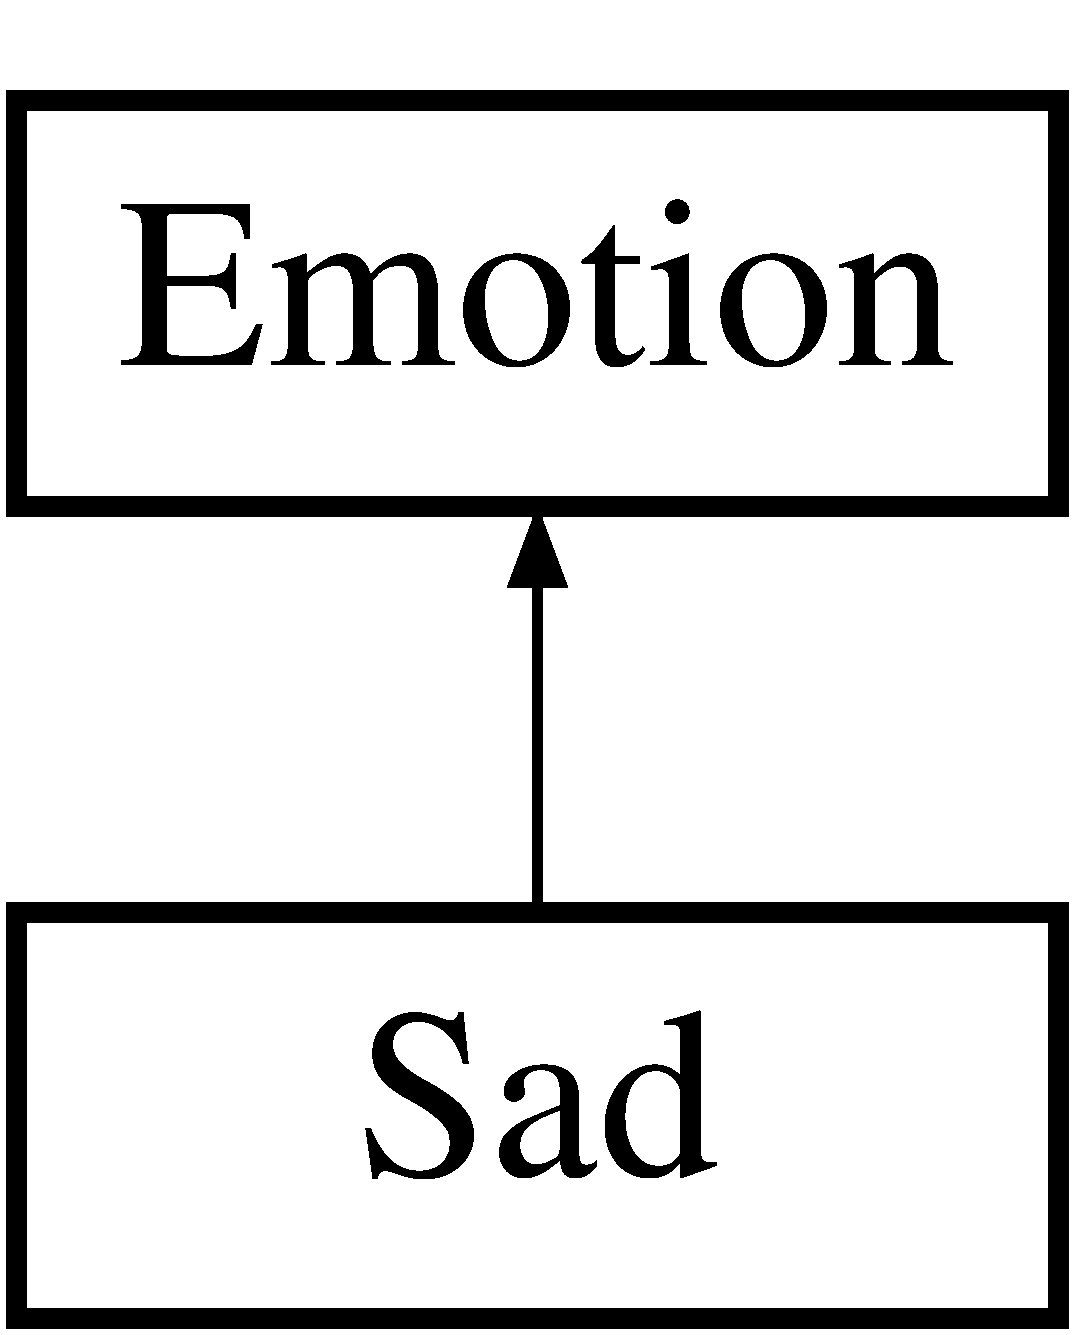
\includegraphics[height=2.000000cm]{class_sad}
\end{center}
\end{figure}
\subsection*{Public Member Functions}
\begin{DoxyCompactItemize}
\item 
\hyperlink{class_sad_aeb827ec6de9543106ac79bb2088701e8}{Sad} (void)
\begin{DoxyCompactList}\small\item\em Default constructor. \end{DoxyCompactList}\item 
\hyperlink{class_sad_a37d84651db69f034d29d1418f0dd023e}{$\sim$\-Sad} (void)
\begin{DoxyCompactList}\small\item\em Destructor. \end{DoxyCompactList}\end{DoxyCompactItemize}


\subsection{Detailed Description}
\hyperlink{class_sad}{Sad}. 

\begin{DoxyAuthor}{Author}
Hamish Carrier 
\end{DoxyAuthor}
\begin{DoxyDate}{Date}
10/11/2013 
\end{DoxyDate}


\subsection{Constructor \& Destructor Documentation}
\hypertarget{class_sad_aeb827ec6de9543106ac79bb2088701e8}{\index{Sad@{Sad}!Sad@{Sad}}
\index{Sad@{Sad}!Sad@{Sad}}
\subsubsection[{Sad}]{\setlength{\rightskip}{0pt plus 5cm}Sad\-::\-Sad (
\begin{DoxyParamCaption}
\item[{void}]{}
\end{DoxyParamCaption}
)}}\label{class_sad_aeb827ec6de9543106ac79bb2088701e8}


Default constructor. 

\begin{DoxyAuthor}{Author}
Hamish Carrier 
\end{DoxyAuthor}
\begin{DoxyDate}{Date}
10/11/2013 
\end{DoxyDate}
\hypertarget{class_sad_a37d84651db69f034d29d1418f0dd023e}{\index{Sad@{Sad}!$\sim$\-Sad@{$\sim$\-Sad}}
\index{$\sim$\-Sad@{$\sim$\-Sad}!Sad@{Sad}}
\subsubsection[{$\sim$\-Sad}]{\setlength{\rightskip}{0pt plus 5cm}Sad\-::$\sim$\-Sad (
\begin{DoxyParamCaption}
\item[{void}]{}
\end{DoxyParamCaption}
)}}\label{class_sad_a37d84651db69f034d29d1418f0dd023e}


Destructor. 

\begin{DoxyAuthor}{Author}
Hamish Carrier 
\end{DoxyAuthor}
\begin{DoxyDate}{Date}
10/11/2013 
\end{DoxyDate}


The documentation for this class was generated from the following files\-:\begin{DoxyCompactItemize}
\item 
A\-:/\-I\-T/\-Git\-Hub/\-I\-C\-T312/source/ogregraphics/\hyperlink{_sad_8h}{Sad.\-h}\item 
A\-:/\-I\-T/\-Git\-Hub/\-I\-C\-T312/source/ogregraphics/Sad.\-cpp\end{DoxyCompactItemize}

\hypertarget{class_scenes_1_1_scene_loader}{\section{Scenes\-:\-:Scene\-Loader Class Reference}
\label{class_scenes_1_1_scene_loader}\index{Scenes\-::\-Scene\-Loader@{Scenes\-::\-Scene\-Loader}}
}
\subsection*{Public Member Functions}
\begin{DoxyCompactItemize}
\item 
\hypertarget{class_scenes_1_1_scene_loader_a476bf8591c9d87f6f4d8707621a48f45}{{\bfseries Scene\-Loader} (\hyperlink{class_scenes_1_1_i_scene}{Scenes\-::\-I\-Scene} $\ast$scene)}\label{class_scenes_1_1_scene_loader_a476bf8591c9d87f6f4d8707621a48f45}

\item 
\hypertarget{class_scenes_1_1_scene_loader_ad8d3d0eeb64c7276d8762bf4b1171041}{bool {\bfseries load\-Scene} (std\-::string scene\-File)}\label{class_scenes_1_1_scene_loader_ad8d3d0eeb64c7276d8762bf4b1171041}

\end{DoxyCompactItemize}


The documentation for this class was generated from the following files\-:\begin{DoxyCompactItemize}
\item 
A\-:/\-I\-T/\-Git\-Hub/\-I\-C\-T312/source/ogregraphics/Scene\-Loader.\-h\item 
A\-:/\-I\-T/\-Git\-Hub/\-I\-C\-T312/source/ogregraphics/Scene\-Loader.\-cpp\end{DoxyCompactItemize}

\hypertarget{class_scenes_1_1_scene_manager}{\section{Scenes\-:\-:Scene\-Manager Class Reference}
\label{class_scenes_1_1_scene_manager}\index{Scenes\-::\-Scene\-Manager@{Scenes\-::\-Scene\-Manager}}
}


Manages the scenes used within the game allowing for changing between scenes, updating scenes and even reverting to the previous scene.  




{\ttfamily \#include $<$Scene\-Manager.\-h$>$}

\subsection*{Public Member Functions}
\begin{DoxyCompactItemize}
\item 
\hypertarget{class_scenes_1_1_scene_manager_a430af5cbeec7a547224ae15a2d21ac89}{\hyperlink{class_scenes_1_1_scene_manager_a430af5cbeec7a547224ae15a2d21ac89}{Scene\-Manager} (void)}\label{class_scenes_1_1_scene_manager_a430af5cbeec7a547224ae15a2d21ac89}

\begin{DoxyCompactList}\small\item\em Default constructor. \end{DoxyCompactList}\item 
\hyperlink{class_scenes_1_1_scene_manager_a003add21b26892729975432b99601af0}{Scene\-Manager} (\hyperlink{class_scenes_1_1_i_scene}{I\-Scene} $\ast$scene)
\begin{DoxyCompactList}\small\item\em Constructor also sets the current scene and initialises it. \end{DoxyCompactList}\item 
\hypertarget{class_scenes_1_1_scene_manager_a710c032c05756e4abe360d6384a4d658}{\hyperlink{class_scenes_1_1_scene_manager_a710c032c05756e4abe360d6384a4d658}{$\sim$\-Scene\-Manager} (void)}\label{class_scenes_1_1_scene_manager_a710c032c05756e4abe360d6384a4d658}

\begin{DoxyCompactList}\small\item\em Destructor. \end{DoxyCompactList}\item 
void \hyperlink{class_scenes_1_1_scene_manager_aaadb1378ac23b3c26c44e6f20626c704}{change\-Scene} (\hyperlink{class_scenes_1_1_i_scene}{I\-Scene} $\ast$scene)
\begin{DoxyCompactList}\small\item\em Changes the current scene to the input scene, exits the previous scene and initialises the new scene. \end{DoxyCompactList}\item 
\hypertarget{class_scenes_1_1_scene_manager_a3e488084d46e3e0805d3fd2852a0cac7}{void \hyperlink{class_scenes_1_1_scene_manager_a3e488084d46e3e0805d3fd2852a0cac7}{revert\-To\-Previous\-Scene} ()}\label{class_scenes_1_1_scene_manager_a3e488084d46e3e0805d3fd2852a0cac7}

\begin{DoxyCompactList}\small\item\em Revert to previous scene. \end{DoxyCompactList}\item 
void \hyperlink{class_scenes_1_1_scene_manager_af9eafb95ed2b49fa867c5b9b45416382}{update\-Scene} (float delta\-Time)
\begin{DoxyCompactList}\small\item\em Updates the current scene passing in the time between frames. \end{DoxyCompactList}\item 
\hypertarget{class_scenes_1_1_scene_manager_a19458b9c99068f3607fb58368f650c2b}{\hyperlink{class_scenes_1_1_i_scene}{Scenes\-::\-I\-Scene} $\ast$ {\bfseries Get\-Scene} ()}\label{class_scenes_1_1_scene_manager_a19458b9c99068f3607fb58368f650c2b}

\end{DoxyCompactItemize}


\subsection{Detailed Description}
Manages the scenes used within the game allowing for changing between scenes, updating scenes and even reverting to the previous scene. 

\begin{DoxyAuthor}{Author}
Timothy Veletta 
\end{DoxyAuthor}
\begin{DoxyDate}{Date}
15/08/13 
\end{DoxyDate}


\subsection{Constructor \& Destructor Documentation}
\hypertarget{class_scenes_1_1_scene_manager_a003add21b26892729975432b99601af0}{\index{Scenes\-::\-Scene\-Manager@{Scenes\-::\-Scene\-Manager}!Scene\-Manager@{Scene\-Manager}}
\index{Scene\-Manager@{Scene\-Manager}!Scenes::SceneManager@{Scenes\-::\-Scene\-Manager}}
\subsubsection[{Scene\-Manager}]{\setlength{\rightskip}{0pt plus 5cm}Scenes\-::\-Scene\-Manager\-::\-Scene\-Manager (
\begin{DoxyParamCaption}
\item[{{\bf I\-Scene} $\ast$}]{scene}
\end{DoxyParamCaption}
)}}\label{class_scenes_1_1_scene_manager_a003add21b26892729975432b99601af0}


Constructor also sets the current scene and initialises it. 


\begin{DoxyParams}[1]{Parameters}
\mbox{\tt in,out}  & {\em scene} & If non-\/null, the scene to be set as current. \\
\hline
\end{DoxyParams}


\subsection{Member Function Documentation}
\hypertarget{class_scenes_1_1_scene_manager_aaadb1378ac23b3c26c44e6f20626c704}{\index{Scenes\-::\-Scene\-Manager@{Scenes\-::\-Scene\-Manager}!change\-Scene@{change\-Scene}}
\index{change\-Scene@{change\-Scene}!Scenes::SceneManager@{Scenes\-::\-Scene\-Manager}}
\subsubsection[{change\-Scene}]{\setlength{\rightskip}{0pt plus 5cm}void Scenes\-::\-Scene\-Manager\-::change\-Scene (
\begin{DoxyParamCaption}
\item[{{\bf I\-Scene} $\ast$}]{scene}
\end{DoxyParamCaption}
)}}\label{class_scenes_1_1_scene_manager_aaadb1378ac23b3c26c44e6f20626c704}


Changes the current scene to the input scene, exits the previous scene and initialises the new scene. 


\begin{DoxyParams}[1]{Parameters}
\mbox{\tt in,out}  & {\em scene} & If non-\/null, the scene to be set as current. \\
\hline
\end{DoxyParams}
\hypertarget{class_scenes_1_1_scene_manager_af9eafb95ed2b49fa867c5b9b45416382}{\index{Scenes\-::\-Scene\-Manager@{Scenes\-::\-Scene\-Manager}!update\-Scene@{update\-Scene}}
\index{update\-Scene@{update\-Scene}!Scenes::SceneManager@{Scenes\-::\-Scene\-Manager}}
\subsubsection[{update\-Scene}]{\setlength{\rightskip}{0pt plus 5cm}void Scenes\-::\-Scene\-Manager\-::update\-Scene (
\begin{DoxyParamCaption}
\item[{float}]{delta\-Time}
\end{DoxyParamCaption}
)}}\label{class_scenes_1_1_scene_manager_af9eafb95ed2b49fa867c5b9b45416382}


Updates the current scene passing in the time between frames. 


\begin{DoxyParams}{Parameters}
{\em delta\-Time} & Time between frames. \\
\hline
\end{DoxyParams}


The documentation for this class was generated from the following files\-:\begin{DoxyCompactItemize}
\item 
A\-:/\-I\-T/\-Git\-Hub/\-I\-C\-T312/source/ogregraphics/Scene\-Manager.\-h\item 
A\-:/\-I\-T/\-Git\-Hub/\-I\-C\-T312/source/ogregraphics/Scene\-Manager.\-cpp\end{DoxyCompactItemize}

\hypertarget{class_sit}{\section{Sit Class Reference}
\label{class_sit}\index{Sit@{Sit}}
}


\hyperlink{class_sit}{Sit}.  




{\ttfamily \#include $<$Sit.\-h$>$}

Inheritance diagram for Sit\-:\begin{figure}[H]
\begin{center}
\leavevmode
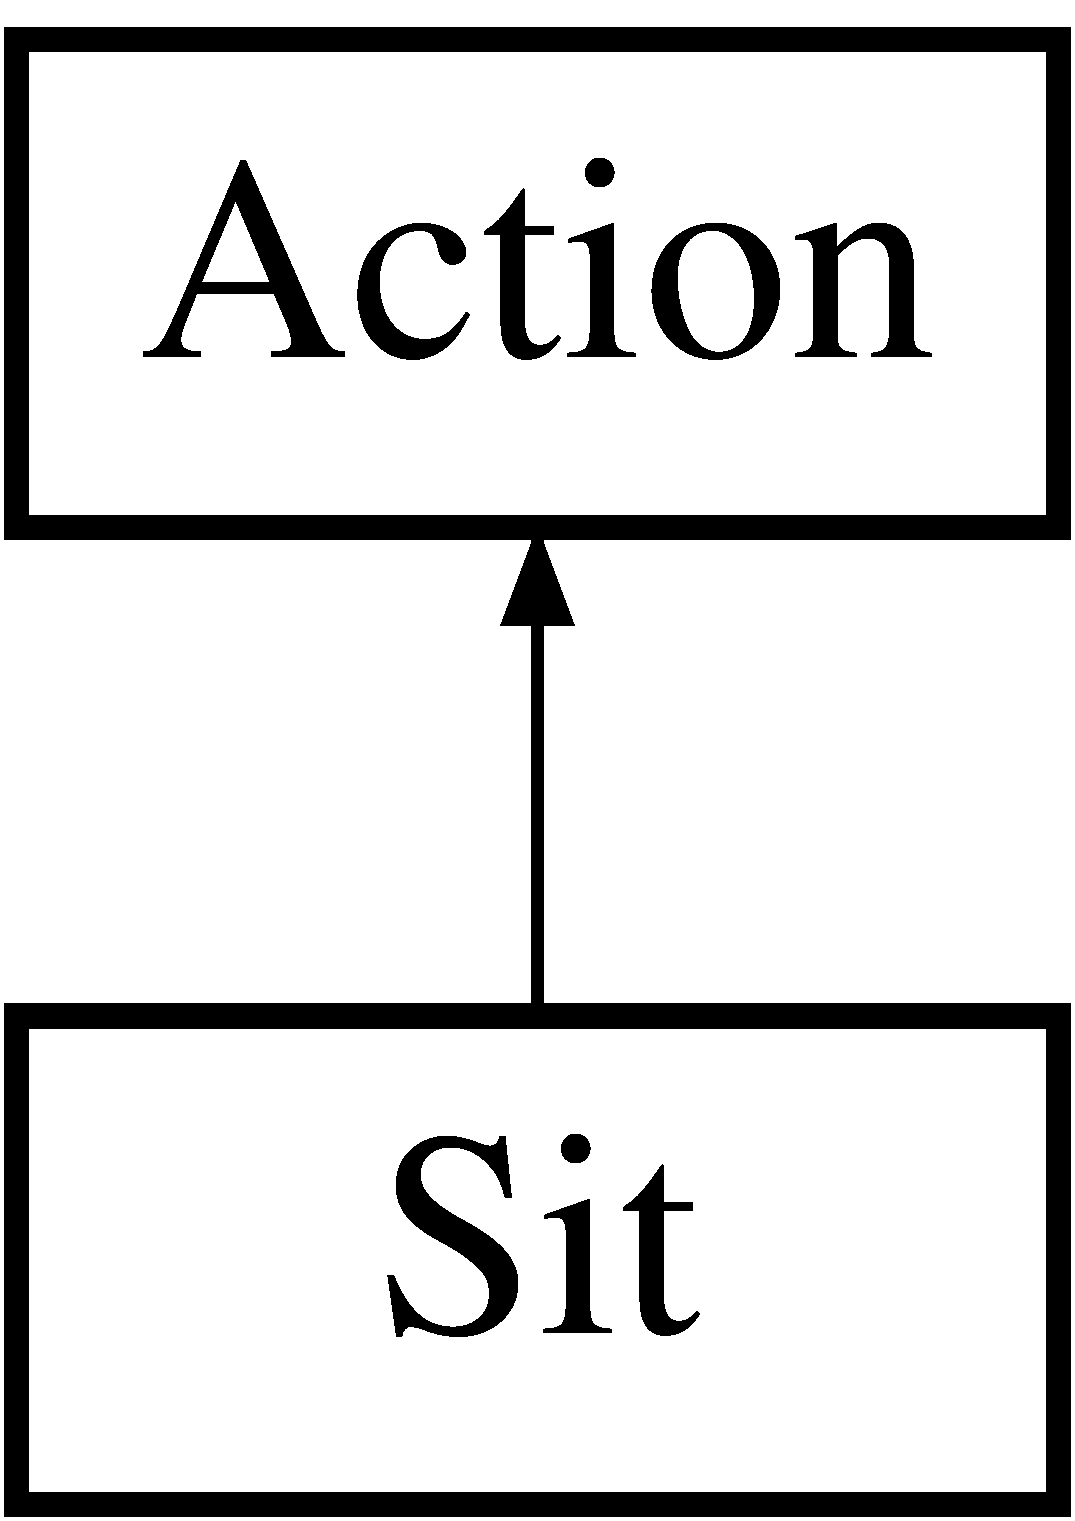
\includegraphics[height=2.000000cm]{class_sit}
\end{center}
\end{figure}
\subsection*{Public Member Functions}
\begin{DoxyCompactItemize}
\item 
\hyperlink{class_sit_a723bf2d8326e2f7fc15f2d938904652a}{Sit} (void)
\begin{DoxyCompactList}\small\item\em Default constructor. \end{DoxyCompactList}\item 
\hyperlink{class_sit_a3b37cc97f31c83b69734bfb2ef66cf00}{$\sim$\-Sit} (void)
\begin{DoxyCompactList}\small\item\em Destructor. \end{DoxyCompactList}\item 
bool \hyperlink{class_sit_a6aa8e20622ce327550627cf0050cb3e6}{Activate} ()
\begin{DoxyCompactList}\small\item\em Activates this object. \end{DoxyCompactList}\end{DoxyCompactItemize}


\subsection{Detailed Description}
\hyperlink{class_sit}{Sit}. 

\begin{DoxyAuthor}{Author}
Hamish Carrier 
\end{DoxyAuthor}
\begin{DoxyDate}{Date}
10/11/2013 
\end{DoxyDate}


\subsection{Constructor \& Destructor Documentation}
\hypertarget{class_sit_a723bf2d8326e2f7fc15f2d938904652a}{\index{Sit@{Sit}!Sit@{Sit}}
\index{Sit@{Sit}!Sit@{Sit}}
\subsubsection[{Sit}]{\setlength{\rightskip}{0pt plus 5cm}Sit\-::\-Sit (
\begin{DoxyParamCaption}
\item[{void}]{}
\end{DoxyParamCaption}
)}}\label{class_sit_a723bf2d8326e2f7fc15f2d938904652a}


Default constructor. 

\begin{DoxyAuthor}{Author}
Hamish Carrier 
\end{DoxyAuthor}
\begin{DoxyDate}{Date}
10/11/2013 
\end{DoxyDate}
\hypertarget{class_sit_a3b37cc97f31c83b69734bfb2ef66cf00}{\index{Sit@{Sit}!$\sim$\-Sit@{$\sim$\-Sit}}
\index{$\sim$\-Sit@{$\sim$\-Sit}!Sit@{Sit}}
\subsubsection[{$\sim$\-Sit}]{\setlength{\rightskip}{0pt plus 5cm}Sit\-::$\sim$\-Sit (
\begin{DoxyParamCaption}
\item[{void}]{}
\end{DoxyParamCaption}
)}}\label{class_sit_a3b37cc97f31c83b69734bfb2ef66cf00}


Destructor. 

\begin{DoxyAuthor}{Author}
Hamish Carrier 
\end{DoxyAuthor}
\begin{DoxyDate}{Date}
10/11/2013 
\end{DoxyDate}


\subsection{Member Function Documentation}
\hypertarget{class_sit_a6aa8e20622ce327550627cf0050cb3e6}{\index{Sit@{Sit}!Activate@{Activate}}
\index{Activate@{Activate}!Sit@{Sit}}
\subsubsection[{Activate}]{\setlength{\rightskip}{0pt plus 5cm}bool Sit\-::\-Activate (
\begin{DoxyParamCaption}
{}
\end{DoxyParamCaption}
)}}\label{class_sit_a6aa8e20622ce327550627cf0050cb3e6}


Activates this object. 

\begin{DoxyAuthor}{Author}
Hamish Carrier 
\end{DoxyAuthor}
\begin{DoxyDate}{Date}
10/11/2013
\end{DoxyDate}
\begin{DoxyReturn}{Returns}
true if it succeeds, false if it fails. 
\end{DoxyReturn}


The documentation for this class was generated from the following files\-:\begin{DoxyCompactItemize}
\item 
A\-:/\-I\-T/\-Git\-Hub/\-I\-C\-T312/source/ogregraphics/\hyperlink{_sit_8h}{Sit.\-h}\item 
A\-:/\-I\-T/\-Git\-Hub/\-I\-C\-T312/source/ogregraphics/Sit.\-cpp\end{DoxyCompactItemize}

\hypertarget{structmicropather_1_1_state_cost}{\section{micropather\-:\-:State\-Cost Struct Reference}
\label{structmicropather_1_1_state_cost}\index{micropather\-::\-State\-Cost@{micropather\-::\-State\-Cost}}
}


{\ttfamily \#include $<$micropather.\-h$>$}

\subsection*{Public Attributes}
\begin{DoxyCompactItemize}
\item 
\hypertarget{structmicropather_1_1_state_cost_aad6ecf700ce5936f129b6ef34e732f97}{void $\ast$ \hyperlink{structmicropather_1_1_state_cost_aad6ecf700ce5936f129b6ef34e732f97}{state}}\label{structmicropather_1_1_state_cost_aad6ecf700ce5936f129b6ef34e732f97}

\begin{DoxyCompactList}\small\item\em The state as a void$\ast$. \end{DoxyCompactList}\item 
\hypertarget{structmicropather_1_1_state_cost_ad66ce8ebce4f7659995c011d0a01c61a}{float \hyperlink{structmicropather_1_1_state_cost_ad66ce8ebce4f7659995c011d0a01c61a}{cost}}\label{structmicropather_1_1_state_cost_ad66ce8ebce4f7659995c011d0a01c61a}

\begin{DoxyCompactList}\small\item\em The cost to the state. Use F\-L\-T\-\_\-\-M\-A\-X for infinite cost. \end{DoxyCompactList}\end{DoxyCompactItemize}


\subsection{Detailed Description}
Used to pass the cost of states from the cliet application to \hyperlink{classmicropather_1_1_micro_pather}{Micro\-Pather}. This structure is copied in a vector.

\begin{DoxySeeAlso}{See Also}
Adjacent\-Cost 
\end{DoxySeeAlso}


The documentation for this struct was generated from the following file\-:\begin{DoxyCompactItemize}
\item 
A\-:/\-I\-T/\-Git\-Hub/\-I\-C\-T312/source/ogregraphics/micropather.\-h\end{DoxyCompactItemize}

\hypertarget{class_ogre_bullet_collisions_1_1_static_mesh_to_shape_converter}{\section{Ogre\-Bullet\-Collisions\-:\-:Static\-Mesh\-To\-Shape\-Converter Class Reference}
\label{class_ogre_bullet_collisions_1_1_static_mesh_to_shape_converter}\index{Ogre\-Bullet\-Collisions\-::\-Static\-Mesh\-To\-Shape\-Converter@{Ogre\-Bullet\-Collisions\-::\-Static\-Mesh\-To\-Shape\-Converter}}
}
Inheritance diagram for Ogre\-Bullet\-Collisions\-:\-:Static\-Mesh\-To\-Shape\-Converter\-:\begin{figure}[H]
\begin{center}
\leavevmode
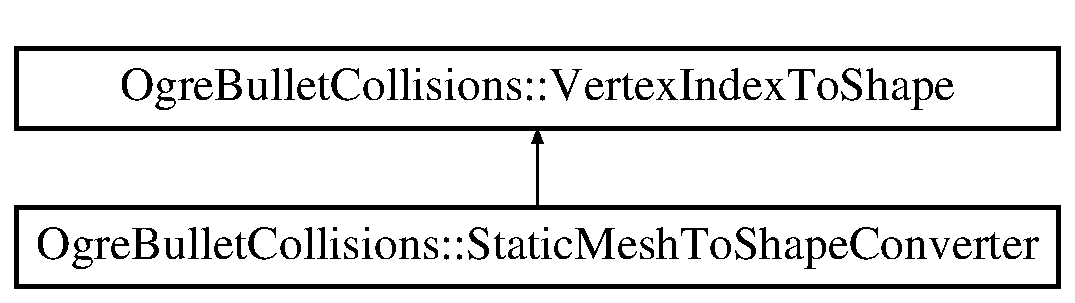
\includegraphics[height=2.000000cm]{class_ogre_bullet_collisions_1_1_static_mesh_to_shape_converter}
\end{center}
\end{figure}
\subsection*{Public Member Functions}
\begin{DoxyCompactItemize}
\item 
\hypertarget{class_ogre_bullet_collisions_1_1_static_mesh_to_shape_converter_a7575a81e2797d6e85119388011d1e26b}{{\bfseries Static\-Mesh\-To\-Shape\-Converter} (Ogre\-::\-Renderable $\ast$rend, const Ogre\-::\-Matrix4 \&transform=Ogre\-::\-Matrix4\-::\-I\-D\-E\-N\-T\-I\-T\-Y)}\label{class_ogre_bullet_collisions_1_1_static_mesh_to_shape_converter_a7575a81e2797d6e85119388011d1e26b}

\item 
\hypertarget{class_ogre_bullet_collisions_1_1_static_mesh_to_shape_converter_a235788ac29af92feb6f162191bf17a82}{{\bfseries Static\-Mesh\-To\-Shape\-Converter} (Ogre\-::\-Entity $\ast$entity, const Ogre\-::\-Matrix4 \&transform=Ogre\-::\-Matrix4\-::\-I\-D\-E\-N\-T\-I\-T\-Y)}\label{class_ogre_bullet_collisions_1_1_static_mesh_to_shape_converter_a235788ac29af92feb6f162191bf17a82}

\item 
\hypertarget{class_ogre_bullet_collisions_1_1_static_mesh_to_shape_converter_ae6cc0c55908320e5ed3d1bd54bc1c22f}{virtual void {\bfseries add\-Entity} (Ogre\-::\-Entity $\ast$entity, const Ogre\-::\-Matrix4 \&transform=Ogre\-::\-Matrix4\-::\-I\-D\-E\-N\-T\-I\-T\-Y)}\label{class_ogre_bullet_collisions_1_1_static_mesh_to_shape_converter_ae6cc0c55908320e5ed3d1bd54bc1c22f}

\item 
\hypertarget{class_ogre_bullet_collisions_1_1_static_mesh_to_shape_converter_a93facb31886ca838c6d7a081bbeddb91}{virtual void {\bfseries add\-Mesh} (const Ogre\-::\-Mesh\-Ptr \&mesh, const Ogre\-::\-Matrix4 \&transform=Ogre\-::\-Matrix4\-::\-I\-D\-E\-N\-T\-I\-T\-Y)}\label{class_ogre_bullet_collisions_1_1_static_mesh_to_shape_converter_a93facb31886ca838c6d7a081bbeddb91}

\end{DoxyCompactItemize}
\subsection*{Protected Attributes}
\begin{DoxyCompactItemize}
\item 
\hypertarget{class_ogre_bullet_collisions_1_1_static_mesh_to_shape_converter_ac4b7cec8cfc349f9f02b4bc031147e08}{Ogre\-::\-Entity $\ast$ {\bfseries m\-Entity}}\label{class_ogre_bullet_collisions_1_1_static_mesh_to_shape_converter_ac4b7cec8cfc349f9f02b4bc031147e08}

\item 
\hypertarget{class_ogre_bullet_collisions_1_1_static_mesh_to_shape_converter_aaf9ad75f5c3b01f2ac11d425229ceab5}{Ogre\-::\-Scene\-Node $\ast$ {\bfseries m\-Node}}\label{class_ogre_bullet_collisions_1_1_static_mesh_to_shape_converter_aaf9ad75f5c3b01f2ac11d425229ceab5}

\end{DoxyCompactItemize}
\subsection*{Additional Inherited Members}


The documentation for this class was generated from the following files\-:\begin{DoxyCompactItemize}
\item 
A\-:/\-I\-T/\-Git\-Hub/\-I\-C\-T312/source/ogregraphics/Ogre\-Bullet\-Collisions\-Mesh\-To\-Shape\-Converter.\-h\item 
A\-:/\-I\-T/\-Git\-Hub/\-I\-C\-T312/source/ogregraphics/Ogre\-Bullet\-Collisions\-Mesh\-To\-Shape\-Converter.\-cpp\end{DoxyCompactItemize}

\hypertarget{class_studious}{\section{Studious Class Reference}
\label{class_studious}\index{Studious@{Studious}}
}


\hyperlink{class_studious}{Studious}.  




{\ttfamily \#include $<$Studious.\-h$>$}

Inheritance diagram for Studious\-:\begin{figure}[H]
\begin{center}
\leavevmode
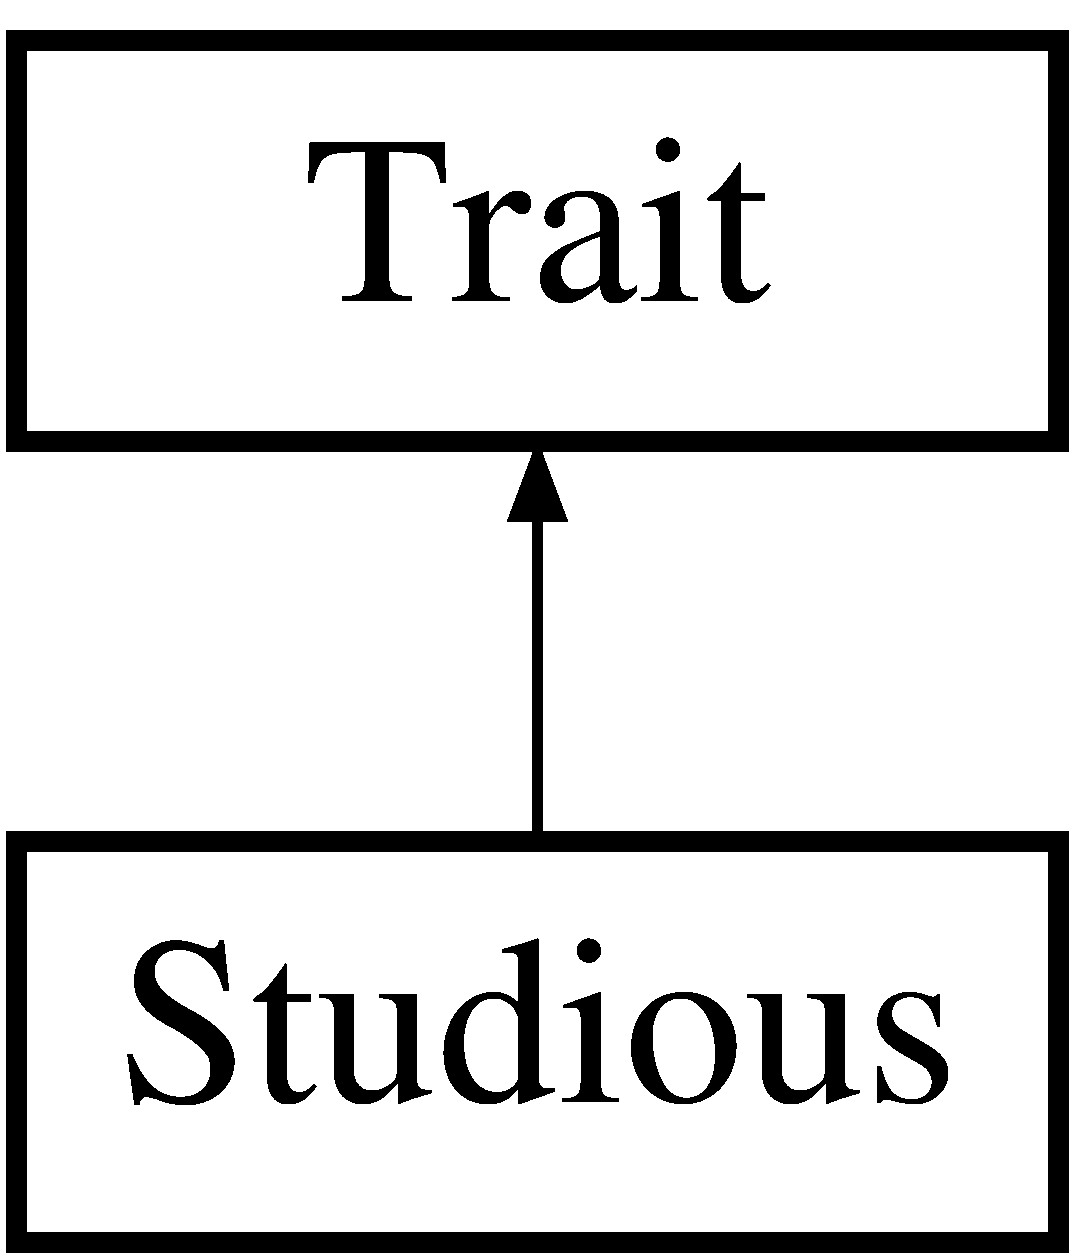
\includegraphics[height=2.000000cm]{class_studious}
\end{center}
\end{figure}
\subsection*{Public Member Functions}
\begin{DoxyCompactItemize}
\item 
\hyperlink{class_studious_a4b7078f053d0c5f70b4fd83f9b191100}{Studious} (void)
\begin{DoxyCompactList}\small\item\em Default constructor. \end{DoxyCompactList}\item 
\hyperlink{class_studious_ac33b2a988b979662ecd4ccec46067c4b}{$\sim$\-Studious} (void)
\begin{DoxyCompactList}\small\item\em Destructor. \end{DoxyCompactList}\end{DoxyCompactItemize}


\subsection{Detailed Description}
\hyperlink{class_studious}{Studious}. 

\begin{DoxyAuthor}{Author}
Hamish Carrier 
\end{DoxyAuthor}
\begin{DoxyDate}{Date}
10/11/2013 
\end{DoxyDate}


\subsection{Constructor \& Destructor Documentation}
\hypertarget{class_studious_a4b7078f053d0c5f70b4fd83f9b191100}{\index{Studious@{Studious}!Studious@{Studious}}
\index{Studious@{Studious}!Studious@{Studious}}
\subsubsection[{Studious}]{\setlength{\rightskip}{0pt plus 5cm}Studious\-::\-Studious (
\begin{DoxyParamCaption}
\item[{void}]{}
\end{DoxyParamCaption}
)}}\label{class_studious_a4b7078f053d0c5f70b4fd83f9b191100}


Default constructor. 

\begin{DoxyAuthor}{Author}
Hamish Carrier 
\end{DoxyAuthor}
\begin{DoxyDate}{Date}
10/11/2013 
\end{DoxyDate}
\hypertarget{class_studious_ac33b2a988b979662ecd4ccec46067c4b}{\index{Studious@{Studious}!$\sim$\-Studious@{$\sim$\-Studious}}
\index{$\sim$\-Studious@{$\sim$\-Studious}!Studious@{Studious}}
\subsubsection[{$\sim$\-Studious}]{\setlength{\rightskip}{0pt plus 5cm}Studious\-::$\sim$\-Studious (
\begin{DoxyParamCaption}
\item[{void}]{}
\end{DoxyParamCaption}
)}}\label{class_studious_ac33b2a988b979662ecd4ccec46067c4b}


Destructor. 

\begin{DoxyAuthor}{Author}
Hamish Carrier 
\end{DoxyAuthor}
\begin{DoxyDate}{Date}
10/11/2013 
\end{DoxyDate}


The documentation for this class was generated from the following files\-:\begin{DoxyCompactItemize}
\item 
A\-:/\-I\-T/\-Git\-Hub/\-I\-C\-T312/source/ogregraphics/\hyperlink{_studious_8h}{Studious.\-h}\item 
A\-:/\-I\-T/\-Git\-Hub/\-I\-C\-T312/source/ogregraphics/Studious.\-cpp\end{DoxyCompactItemize}

\hypertarget{class_objects_1_1_target_object}{\section{Objects\-:\-:Target\-Object Class Reference}
\label{class_objects_1_1_target_object}\index{Objects\-::\-Target\-Object@{Objects\-::\-Target\-Object}}
}
Inheritance diagram for Objects\-:\-:Target\-Object\-:\begin{figure}[H]
\begin{center}
\leavevmode
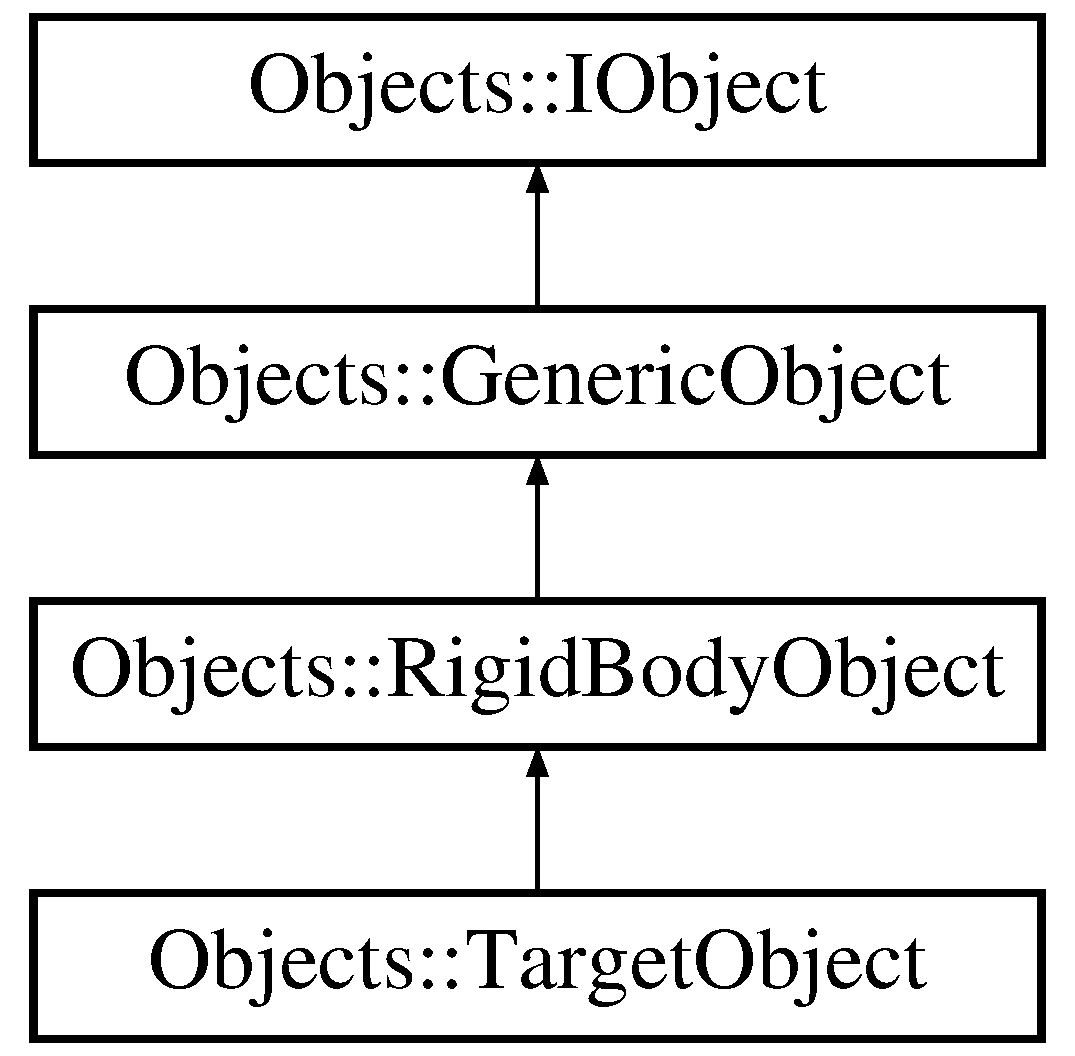
\includegraphics[height=4.000000cm]{class_objects_1_1_target_object}
\end{center}
\end{figure}
\subsection*{Public Member Functions}
\begin{DoxyCompactItemize}
\item 
\hypertarget{class_objects_1_1_target_object_adff3ad3f9d68c1c323ebcb06679c7549}{virtual void \hyperlink{class_objects_1_1_target_object_adff3ad3f9d68c1c323ebcb06679c7549}{initialise} ()}\label{class_objects_1_1_target_object_adff3ad3f9d68c1c323ebcb06679c7549}

\begin{DoxyCompactList}\small\item\em Initialises this object. \end{DoxyCompactList}\item 
virtual void \hyperlink{class_objects_1_1_target_object_a46b8163c5921925aa6d95fc0e99ce011}{update} (float delta\-Time)
\begin{DoxyCompactList}\small\item\em Updates the given delta\-Time. \end{DoxyCompactList}\end{DoxyCompactItemize}
\subsection*{Additional Inherited Members}


\subsection{Member Function Documentation}
\hypertarget{class_objects_1_1_target_object_a46b8163c5921925aa6d95fc0e99ce011}{\index{Objects\-::\-Target\-Object@{Objects\-::\-Target\-Object}!update@{update}}
\index{update@{update}!Objects::TargetObject@{Objects\-::\-Target\-Object}}
\subsubsection[{update}]{\setlength{\rightskip}{0pt plus 5cm}void Target\-Object\-::update (
\begin{DoxyParamCaption}
\item[{float}]{delta\-Time}
\end{DoxyParamCaption}
)\hspace{0.3cm}{\ttfamily [virtual]}}}\label{class_objects_1_1_target_object_a46b8163c5921925aa6d95fc0e99ce011}


Updates the given delta\-Time. 


\begin{DoxyParams}{Parameters}
{\em delta\-Time} & Time of the delta. \\
\hline
\end{DoxyParams}


Reimplemented from \hyperlink{class_objects_1_1_rigid_body_object_a478edcbc5820722a9641fdcd07b402bb}{Objects\-::\-Rigid\-Body\-Object}.



The documentation for this class was generated from the following files\-:\begin{DoxyCompactItemize}
\item 
A\-:/\-I\-T/\-Git\-Hub/\-I\-C\-T312/source/ogregraphics/Target\-Object.\-h\item 
A\-:/\-I\-T/\-Git\-Hub/\-I\-C\-T312/source/ogregraphics/Target\-Object.\-cpp\end{DoxyCompactItemize}

\hypertarget{class_temporary_player_object}{\section{Temporary\-Player\-Object Class Reference}
\label{class_temporary_player_object}\index{Temporary\-Player\-Object@{Temporary\-Player\-Object}}
}
\subsection*{Public Member Functions}
\begin{DoxyCompactItemize}
\item 
\hypertarget{class_temporary_player_object_af3be5d8902a89f95880ee913e77f4de4}{void {\bfseries Set\-Last\-Pos} (float posx, float posy, float posz)}\label{class_temporary_player_object_af3be5d8902a89f95880ee913e77f4de4}

\end{DoxyCompactItemize}
\subsection*{Public Attributes}
\begin{DoxyCompactItemize}
\item 
\hypertarget{class_temporary_player_object_a75290f421231aee09006f2caee75283e}{Ogre\-::\-Vector3 {\bfseries lastposition}}\label{class_temporary_player_object_a75290f421231aee09006f2caee75283e}

\end{DoxyCompactItemize}


The documentation for this class was generated from the following files\-:\begin{DoxyCompactItemize}
\item 
A\-:/\-I\-T/\-Git\-Hub/\-I\-C\-T312/source/ogregraphics/Temporary\-Player\-Object.\-h\item 
A\-:/\-I\-T/\-Git\-Hub/\-I\-C\-T312/source/ogregraphics/Temporary\-Player\-Object.\-cpp\end{DoxyCompactItemize}

\hypertarget{class_objects_1_1_test_object}{\section{Objects\-:\-:Test\-Object Class Reference}
\label{class_objects_1_1_test_object}\index{Objects\-::\-Test\-Object@{Objects\-::\-Test\-Object}}
}
Inheritance diagram for Objects\-:\-:Test\-Object\-:\begin{figure}[H]
\begin{center}
\leavevmode
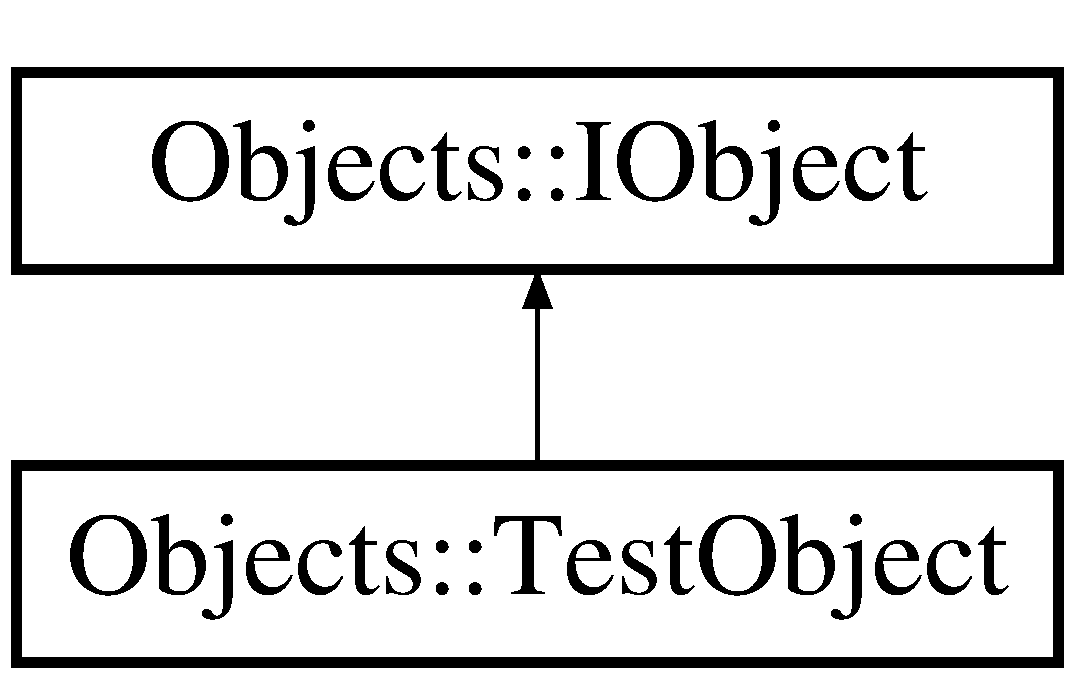
\includegraphics[height=2.000000cm]{class_objects_1_1_test_object}
\end{center}
\end{figure}
\subsection*{Public Member Functions}
\begin{DoxyCompactItemize}
\item 
\hypertarget{class_objects_1_1_test_object_aaca6ace404d3d0c889284bb189370007}{virtual void \hyperlink{class_objects_1_1_test_object_aaca6ace404d3d0c889284bb189370007}{initialise} ()}\label{class_objects_1_1_test_object_aaca6ace404d3d0c889284bb189370007}

\begin{DoxyCompactList}\small\item\em Initialises this object. \end{DoxyCompactList}\item 
virtual void \hyperlink{class_objects_1_1_test_object_a5df5df31f7f1233cd991d200ecac7205}{update} (float delta\-Time)
\begin{DoxyCompactList}\small\item\em Updates the given delta\-Time. \end{DoxyCompactList}\end{DoxyCompactItemize}
\subsection*{Additional Inherited Members}


\subsection{Member Function Documentation}
\hypertarget{class_objects_1_1_test_object_a5df5df31f7f1233cd991d200ecac7205}{\index{Objects\-::\-Test\-Object@{Objects\-::\-Test\-Object}!update@{update}}
\index{update@{update}!Objects::TestObject@{Objects\-::\-Test\-Object}}
\subsubsection[{update}]{\setlength{\rightskip}{0pt plus 5cm}void Test\-Object\-::update (
\begin{DoxyParamCaption}
\item[{float}]{delta\-Time}
\end{DoxyParamCaption}
)\hspace{0.3cm}{\ttfamily [virtual]}}}\label{class_objects_1_1_test_object_a5df5df31f7f1233cd991d200ecac7205}


Updates the given delta\-Time. 


\begin{DoxyParams}{Parameters}
{\em delta\-Time} & Time of the delta. \\
\hline
\end{DoxyParams}


Reimplemented from \hyperlink{class_objects_1_1_i_object_a616e6befc5fbdca47155b1b56d0e0fc0}{Objects\-::\-I\-Object}.



The documentation for this class was generated from the following files\-:\begin{DoxyCompactItemize}
\item 
A\-:/\-I\-T/\-Git\-Hub/\-I\-C\-T312/source/ogregraphics/Test\-Object.\-h\item 
A\-:/\-I\-T/\-Git\-Hub/\-I\-C\-T312/source/ogregraphics/Test\-Object.\-cpp\end{DoxyCompactItemize}

\hypertarget{class_test_scene}{\section{Test\-Scene Class Reference}
\label{class_test_scene}\index{Test\-Scene@{Test\-Scene}}
}
Inheritance diagram for Test\-Scene\-:\begin{figure}[H]
\begin{center}
\leavevmode
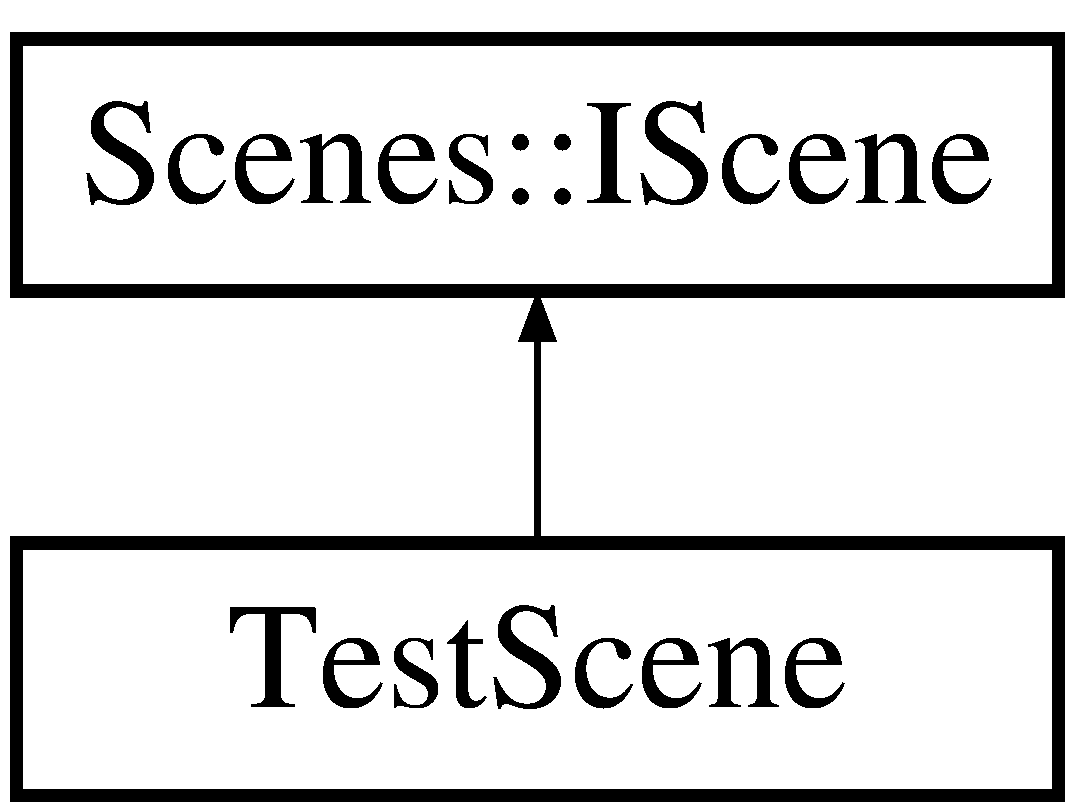
\includegraphics[height=2.000000cm]{class_test_scene}
\end{center}
\end{figure}
\subsection*{Public Member Functions}
\begin{DoxyCompactItemize}
\item 
\hypertarget{class_test_scene_af421b86202de66b69b3c21870e1ee990}{virtual void \hyperlink{class_test_scene_af421b86202de66b69b3c21870e1ee990}{initialise} ()}\label{class_test_scene_af421b86202de66b69b3c21870e1ee990}

\begin{DoxyCompactList}\small\item\em Initialises this object. \end{DoxyCompactList}\item 
virtual void \hyperlink{class_test_scene_ad42240fabf5883d481191871cc91c5c3}{update} (float delta\-Time)
\begin{DoxyCompactList}\small\item\em Updates the scene given the change in time from one frame to another. \end{DoxyCompactList}\item 
\hypertarget{class_test_scene_aec5414397def44e25bbc11b9631ec959}{virtual void \hyperlink{class_test_scene_aec5414397def44e25bbc11b9631ec959}{on\-Exit} ()}\label{class_test_scene_aec5414397def44e25bbc11b9631ec959}

\begin{DoxyCompactList}\small\item\em Executes the exit action. \end{DoxyCompactList}\end{DoxyCompactItemize}


\subsection{Member Function Documentation}
\hypertarget{class_test_scene_ad42240fabf5883d481191871cc91c5c3}{\index{Test\-Scene@{Test\-Scene}!update@{update}}
\index{update@{update}!TestScene@{Test\-Scene}}
\subsubsection[{update}]{\setlength{\rightskip}{0pt plus 5cm}void Test\-Scene\-::update (
\begin{DoxyParamCaption}
\item[{float}]{delta\-Time}
\end{DoxyParamCaption}
)\hspace{0.3cm}{\ttfamily [virtual]}}}\label{class_test_scene_ad42240fabf5883d481191871cc91c5c3}


Updates the scene given the change in time from one frame to another. 


\begin{DoxyParams}{Parameters}
{\em delta\-Time} & The change in time from one frame to another. \\
\hline
\end{DoxyParams}


Reimplemented from \hyperlink{class_scenes_1_1_i_scene_acb97c42a9a93ce1b3d0b800bda680935}{Scenes\-::\-I\-Scene}.



The documentation for this class was generated from the following files\-:\begin{DoxyCompactItemize}
\item 
A\-:/\-I\-T/\-Git\-Hub/\-I\-C\-T312/source/ogregraphics/\hyperlink{_test_scene_8h}{Test\-Scene.\-h}\item 
A\-:/\-I\-T/\-Git\-Hub/\-I\-C\-T312/source/ogregraphics/Test\-Scene.\-cpp\end{DoxyCompactItemize}

\hypertarget{class_trait}{\section{Trait Class Reference}
\label{class_trait}\index{Trait@{Trait}}
}


\hyperlink{class_trait}{Trait}.  




{\ttfamily \#include $<$Trait.\-h$>$}

Inheritance diagram for Trait\-:\begin{figure}[H]
\begin{center}
\leavevmode
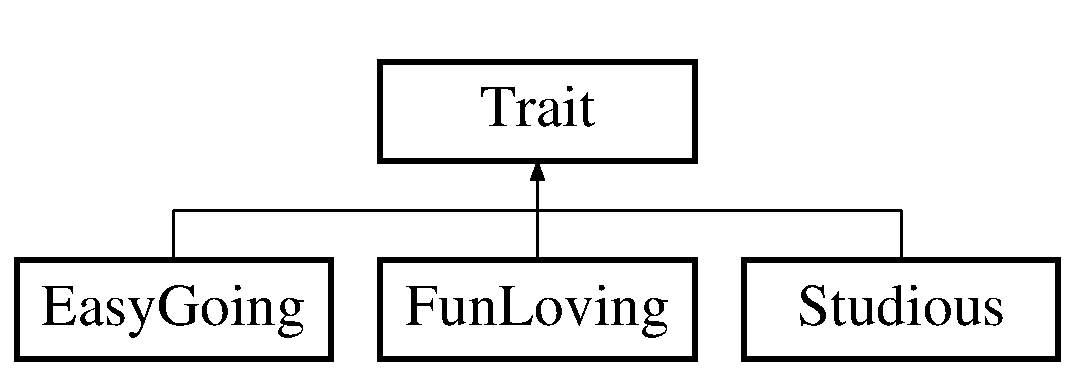
\includegraphics[height=2.000000cm]{class_trait}
\end{center}
\end{figure}


\subsection{Detailed Description}
\hyperlink{class_trait}{Trait}. 

\begin{DoxyAuthor}{Author}
Hamish Carrier 
\end{DoxyAuthor}
\begin{DoxyDate}{Date}
10/11/2013 
\end{DoxyDate}


The documentation for this class was generated from the following file\-:\begin{DoxyCompactItemize}
\item 
A\-:/\-I\-T/\-Git\-Hub/\-I\-C\-T312/source/ogregraphics/\hyperlink{_trait_8h}{Trait.\-h}\end{DoxyCompactItemize}

\hypertarget{struct_ico_sphere_1_1_triangle_indices}{\section{Ico\-Sphere\-:\-:Triangle\-Indices Struct Reference}
\label{struct_ico_sphere_1_1_triangle_indices}\index{Ico\-Sphere\-::\-Triangle\-Indices@{Ico\-Sphere\-::\-Triangle\-Indices}}
}
\subsection*{Public Member Functions}
\begin{DoxyCompactItemize}
\item 
\hypertarget{struct_ico_sphere_1_1_triangle_indices_ab081d7fcd29a87968cb6f4eaf0a191fd}{{\bfseries Triangle\-Indices} (int \-\_\-v1, int \-\_\-v2, int \-\_\-v3)}\label{struct_ico_sphere_1_1_triangle_indices_ab081d7fcd29a87968cb6f4eaf0a191fd}

\item 
\hypertarget{struct_ico_sphere_1_1_triangle_indices_a0433cdbccce9d48b0f55e2d3256666cf}{bool {\bfseries operator$<$} (const \hyperlink{struct_ico_sphere_1_1_triangle_indices}{Triangle\-Indices} \&o) const }\label{struct_ico_sphere_1_1_triangle_indices_a0433cdbccce9d48b0f55e2d3256666cf}

\end{DoxyCompactItemize}
\subsection*{Public Attributes}
\begin{DoxyCompactItemize}
\item 
\hypertarget{struct_ico_sphere_1_1_triangle_indices_a6b867bfc7660d478b034db0f7c9b5eaa}{int {\bfseries v1}}\label{struct_ico_sphere_1_1_triangle_indices_a6b867bfc7660d478b034db0f7c9b5eaa}

\item 
\hypertarget{struct_ico_sphere_1_1_triangle_indices_ac9c7858fe1c8ffc4f99b417954d53bef}{int {\bfseries v2}}\label{struct_ico_sphere_1_1_triangle_indices_ac9c7858fe1c8ffc4f99b417954d53bef}

\item 
\hypertarget{struct_ico_sphere_1_1_triangle_indices_ac70983c073b90f99a48ccab911f35638}{int {\bfseries v3}}\label{struct_ico_sphere_1_1_triangle_indices_ac70983c073b90f99a48ccab911f35638}

\end{DoxyCompactItemize}


The documentation for this struct was generated from the following file\-:\begin{DoxyCompactItemize}
\item 
A\-:/\-I\-T/\-Git\-Hub/\-I\-C\-T312/source/ogregraphics/Debug\-Drawer.\-h\end{DoxyCompactItemize}

\hypertarget{class_use_computer}{\section{Use\-Computer Class Reference}
\label{class_use_computer}\index{Use\-Computer@{Use\-Computer}}
}


Use computer.  




{\ttfamily \#include $<$Use\-Computer.\-h$>$}

Inheritance diagram for Use\-Computer\-:\begin{figure}[H]
\begin{center}
\leavevmode
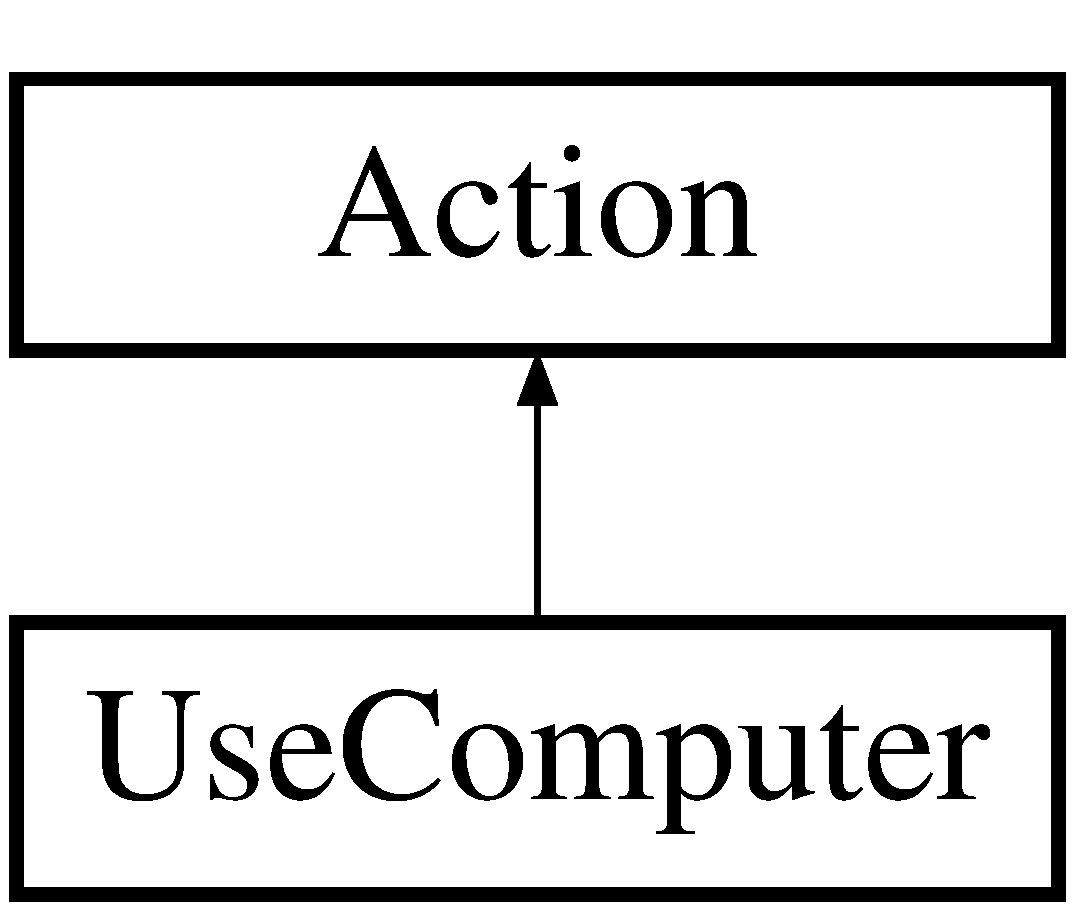
\includegraphics[height=2.000000cm]{class_use_computer}
\end{center}
\end{figure}
\subsection*{Public Member Functions}
\begin{DoxyCompactItemize}
\item 
\hyperlink{class_use_computer_a54797cbaae3ce098f91540d548518a1d}{Use\-Computer} (void)
\begin{DoxyCompactList}\small\item\em Default constructor. \end{DoxyCompactList}\item 
\hyperlink{class_use_computer_a7d2d5695d2e44354885449acecc9ccd9}{$\sim$\-Use\-Computer} (void)
\begin{DoxyCompactList}\small\item\em Destructor. \end{DoxyCompactList}\item 
bool \hyperlink{class_use_computer_aaf6ac208d69b137163324657dd97cf10}{Activate} ()
\begin{DoxyCompactList}\small\item\em Activates this object. \end{DoxyCompactList}\end{DoxyCompactItemize}


\subsection{Detailed Description}
Use computer. 

\begin{DoxyAuthor}{Author}
Hamish Carrier 
\end{DoxyAuthor}
\begin{DoxyDate}{Date}
10/11/2013 
\end{DoxyDate}


\subsection{Constructor \& Destructor Documentation}
\hypertarget{class_use_computer_a54797cbaae3ce098f91540d548518a1d}{\index{Use\-Computer@{Use\-Computer}!Use\-Computer@{Use\-Computer}}
\index{Use\-Computer@{Use\-Computer}!UseComputer@{Use\-Computer}}
\subsubsection[{Use\-Computer}]{\setlength{\rightskip}{0pt plus 5cm}Use\-Computer\-::\-Use\-Computer (
\begin{DoxyParamCaption}
\item[{void}]{}
\end{DoxyParamCaption}
)}}\label{class_use_computer_a54797cbaae3ce098f91540d548518a1d}


Default constructor. 

\begin{DoxyAuthor}{Author}
Hamish Carrier 
\end{DoxyAuthor}
\begin{DoxyDate}{Date}
10/11/2013 
\end{DoxyDate}
\hypertarget{class_use_computer_a7d2d5695d2e44354885449acecc9ccd9}{\index{Use\-Computer@{Use\-Computer}!$\sim$\-Use\-Computer@{$\sim$\-Use\-Computer}}
\index{$\sim$\-Use\-Computer@{$\sim$\-Use\-Computer}!UseComputer@{Use\-Computer}}
\subsubsection[{$\sim$\-Use\-Computer}]{\setlength{\rightskip}{0pt plus 5cm}Use\-Computer\-::$\sim$\-Use\-Computer (
\begin{DoxyParamCaption}
\item[{void}]{}
\end{DoxyParamCaption}
)}}\label{class_use_computer_a7d2d5695d2e44354885449acecc9ccd9}


Destructor. 

\begin{DoxyAuthor}{Author}
Hamish Carrier 
\end{DoxyAuthor}
\begin{DoxyDate}{Date}
10/11/2013 
\end{DoxyDate}


\subsection{Member Function Documentation}
\hypertarget{class_use_computer_aaf6ac208d69b137163324657dd97cf10}{\index{Use\-Computer@{Use\-Computer}!Activate@{Activate}}
\index{Activate@{Activate}!UseComputer@{Use\-Computer}}
\subsubsection[{Activate}]{\setlength{\rightskip}{0pt plus 5cm}bool Use\-Computer\-::\-Activate (
\begin{DoxyParamCaption}
{}
\end{DoxyParamCaption}
)}}\label{class_use_computer_aaf6ac208d69b137163324657dd97cf10}


Activates this object. 

\begin{DoxyAuthor}{Author}
Hamish Carrier 
\end{DoxyAuthor}
\begin{DoxyDate}{Date}
10/11/2013
\end{DoxyDate}
\begin{DoxyReturn}{Returns}
true if it succeeds, false if it fails. 
\end{DoxyReturn}


The documentation for this class was generated from the following files\-:\begin{DoxyCompactItemize}
\item 
A\-:/\-I\-T/\-Git\-Hub/\-I\-C\-T312/source/ogregraphics/\hyperlink{_use_computer_8h}{Use\-Computer.\-h}\item 
A\-:/\-I\-T/\-Git\-Hub/\-I\-C\-T312/source/ogregraphics/Use\-Computer.\-cpp\end{DoxyCompactItemize}

\hypertarget{struct_math_1_1_vector3}{\section{Math\-:\-:Vector3 Struct Reference}
\label{struct_math_1_1_vector3}\index{Math\-::\-Vector3@{Math\-::\-Vector3}}
}
\subsection*{Public Member Functions}
\begin{DoxyCompactItemize}
\item 
\hypertarget{struct_math_1_1_vector3_ac7620e32edb2e7c4c0723b9721ffc23a}{{\bfseries Vector3} (float x, float y, float z)}\label{struct_math_1_1_vector3_ac7620e32edb2e7c4c0723b9721ffc23a}

\item 
\hypertarget{struct_math_1_1_vector3_afbfdb69cef54e84d72d05c3c141e315f}{\hyperlink{struct_math_1_1_vector3}{Vector3} \& {\bfseries operator=} (const \hyperlink{struct_math_1_1_vector3}{Vector3} \&rhs)}\label{struct_math_1_1_vector3_afbfdb69cef54e84d72d05c3c141e315f}

\item 
\hypertarget{struct_math_1_1_vector3_a339c80afd026abb2e35a4ae88301928b}{\hyperlink{struct_math_1_1_vector3}{Vector3} \& {\bfseries operator+=} (const \hyperlink{struct_math_1_1_vector3}{Vector3} \&rhs)}\label{struct_math_1_1_vector3_a339c80afd026abb2e35a4ae88301928b}

\item 
\hypertarget{struct_math_1_1_vector3_a11647e19301236797d60d705e7ce3fda}{\hyperlink{struct_math_1_1_vector3}{Vector3} \& {\bfseries operator$\ast$} (const float rhs)}\label{struct_math_1_1_vector3_a11647e19301236797d60d705e7ce3fda}

\item 
\hypertarget{struct_math_1_1_vector3_af68bf47c957410d436e53de3e6633fbd}{Ogre\-::\-Vector3 {\bfseries to\-Ogre} () const }\label{struct_math_1_1_vector3_af68bf47c957410d436e53de3e6633fbd}

\end{DoxyCompactItemize}
\subsection*{Public Attributes}
\begin{DoxyCompactItemize}
\item 
\hypertarget{struct_math_1_1_vector3_a878843e917c48787b4e1fcffa8b4da3b}{float {\bfseries x}}\label{struct_math_1_1_vector3_a878843e917c48787b4e1fcffa8b4da3b}

\item 
\hypertarget{struct_math_1_1_vector3_a5d4c7c63b32834eb022f57965a1035f2}{float {\bfseries y}}\label{struct_math_1_1_vector3_a5d4c7c63b32834eb022f57965a1035f2}

\item 
\hypertarget{struct_math_1_1_vector3_a425203878d04e4e15de18527a4d3cd0f}{float {\bfseries z}}\label{struct_math_1_1_vector3_a425203878d04e4e15de18527a4d3cd0f}

\end{DoxyCompactItemize}


The documentation for this struct was generated from the following files\-:\begin{DoxyCompactItemize}
\item 
A\-:/\-I\-T/\-Git\-Hub/\-I\-C\-T312/source/ogregraphics/Vector3.\-h\item 
A\-:/\-I\-T/\-Git\-Hub/\-I\-C\-T312/source/ogregraphics/Vector3.\-cpp\end{DoxyCompactItemize}

\hypertarget{class_ogre_bullet_collisions_1_1_vertex_index_to_shape}{\section{Ogre\-Bullet\-Collisions\-:\-:Vertex\-Index\-To\-Shape Class Reference}
\label{class_ogre_bullet_collisions_1_1_vertex_index_to_shape}\index{Ogre\-Bullet\-Collisions\-::\-Vertex\-Index\-To\-Shape@{Ogre\-Bullet\-Collisions\-::\-Vertex\-Index\-To\-Shape}}
}
Inheritance diagram for Ogre\-Bullet\-Collisions\-:\-:Vertex\-Index\-To\-Shape\-:\begin{figure}[H]
\begin{center}
\leavevmode
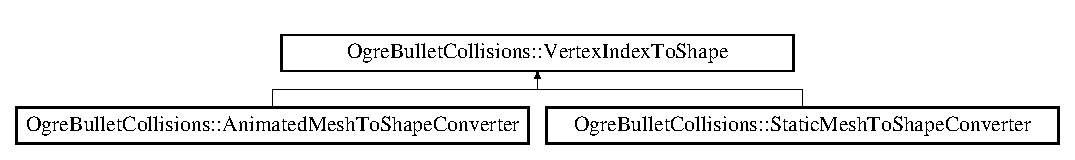
\includegraphics[height=1.696970cm]{class_ogre_bullet_collisions_1_1_vertex_index_to_shape}
\end{center}
\end{figure}
\subsection*{Public Member Functions}
\begin{DoxyCompactItemize}
\item 
\hypertarget{class_ogre_bullet_collisions_1_1_vertex_index_to_shape_a36d2670067e80360990c55aafe47901c}{{\bfseries Vertex\-Index\-To\-Shape} (const Ogre\-::\-Matrix4 \&transform=Ogre\-::\-Matrix4\-::\-I\-D\-E\-N\-T\-I\-T\-Y)}\label{class_ogre_bullet_collisions_1_1_vertex_index_to_shape_a36d2670067e80360990c55aafe47901c}

\item 
\hypertarget{class_ogre_bullet_collisions_1_1_vertex_index_to_shape_a820684f6bfeab961a407fbfc3a519dab}{Ogre\-::\-Real {\bfseries get\-Radius} ()}\label{class_ogre_bullet_collisions_1_1_vertex_index_to_shape_a820684f6bfeab961a407fbfc3a519dab}

\item 
\hypertarget{class_ogre_bullet_collisions_1_1_vertex_index_to_shape_afeb7937345c7eb1ef19db4ff0c189120}{Ogre\-::\-Vector3 {\bfseries get\-Size} ()}\label{class_ogre_bullet_collisions_1_1_vertex_index_to_shape_afeb7937345c7eb1ef19db4ff0c189120}

\item 
\hypertarget{class_ogre_bullet_collisions_1_1_vertex_index_to_shape_a33117e31a4277a8ff4496dd8fe5d2a9a}{Sphere\-Collision\-Shape $\ast$ {\bfseries create\-Sphere} ()}\label{class_ogre_bullet_collisions_1_1_vertex_index_to_shape_a33117e31a4277a8ff4496dd8fe5d2a9a}

\item 
\hypertarget{class_ogre_bullet_collisions_1_1_vertex_index_to_shape_a1b3902e976cb0b37cd3b854db4eba7a8}{Box\-Collision\-Shape $\ast$ {\bfseries create\-Box} ()}\label{class_ogre_bullet_collisions_1_1_vertex_index_to_shape_a1b3902e976cb0b37cd3b854db4eba7a8}

\item 
\hypertarget{class_ogre_bullet_collisions_1_1_vertex_index_to_shape_aa85c20fdb426b5939d036116685b3545}{Triangle\-Mesh\-Collision\-Shape $\ast$ {\bfseries create\-Trimesh} ()}\label{class_ogre_bullet_collisions_1_1_vertex_index_to_shape_aa85c20fdb426b5939d036116685b3545}

\item 
\hypertarget{class_ogre_bullet_collisions_1_1_vertex_index_to_shape_ad61881f4888db1fb5b8b27d8b29dc72f}{Cylinder\-Collision\-Shape $\ast$ {\bfseries create\-Cylinder} ()}\label{class_ogre_bullet_collisions_1_1_vertex_index_to_shape_ad61881f4888db1fb5b8b27d8b29dc72f}

\item 
\hypertarget{class_ogre_bullet_collisions_1_1_vertex_index_to_shape_af2c2aac0df263aafd10f041b5c7649f6}{Convex\-Hull\-Collision\-Shape $\ast$ {\bfseries create\-Convex} ()}\label{class_ogre_bullet_collisions_1_1_vertex_index_to_shape_af2c2aac0df263aafd10f041b5c7649f6}

\item 
\hypertarget{class_ogre_bullet_collisions_1_1_vertex_index_to_shape_a08c44ff9ef91709bfa39bf415ff68b94}{G\-Impact\-Concave\-Shape $\ast$ {\bfseries create\-Concave} ()}\label{class_ogre_bullet_collisions_1_1_vertex_index_to_shape_a08c44ff9ef91709bfa39bf415ff68b94}

\item 
\hypertarget{class_ogre_bullet_collisions_1_1_vertex_index_to_shape_a52422ded2bfa86116982ca05890e3443}{Compound\-Collision\-Shape $\ast$ {\bfseries create\-Convex\-Decomposition} (unsigned int depth=5, float cpercent=5, float ppercent=15, unsigned int maxv=32, float skin\-Width=0.\-0)}\label{class_ogre_bullet_collisions_1_1_vertex_index_to_shape_a52422ded2bfa86116982ca05890e3443}

\item 
\hypertarget{class_ogre_bullet_collisions_1_1_vertex_index_to_shape_a68f239cf3ff4bd626a2b68f46de23025}{const Ogre\-::\-Vector3 $\ast$ {\bfseries get\-Vertices} ()}\label{class_ogre_bullet_collisions_1_1_vertex_index_to_shape_a68f239cf3ff4bd626a2b68f46de23025}

\item 
\hypertarget{class_ogre_bullet_collisions_1_1_vertex_index_to_shape_a0b60b172c1e7156cbf40edc15e63296e}{unsigned int {\bfseries get\-Vertex\-Count} ()}\label{class_ogre_bullet_collisions_1_1_vertex_index_to_shape_a0b60b172c1e7156cbf40edc15e63296e}

\item 
\hypertarget{class_ogre_bullet_collisions_1_1_vertex_index_to_shape_a0330c32a23c640c76c552a7b14bfcdd8}{const unsigned int $\ast$ {\bfseries get\-Indices} ()}\label{class_ogre_bullet_collisions_1_1_vertex_index_to_shape_a0330c32a23c640c76c552a7b14bfcdd8}

\item 
\hypertarget{class_ogre_bullet_collisions_1_1_vertex_index_to_shape_a3b70612d9c85ebe7a56de6c3ad81a963}{unsigned int {\bfseries get\-Index\-Count} ()}\label{class_ogre_bullet_collisions_1_1_vertex_index_to_shape_a3b70612d9c85ebe7a56de6c3ad81a963}

\end{DoxyCompactItemize}
\subsection*{Protected Member Functions}
\begin{DoxyCompactItemize}
\item 
\hypertarget{class_ogre_bullet_collisions_1_1_vertex_index_to_shape_a8c91f06cebd3c8a5d35f8c38fb133bd6}{void {\bfseries add\-Static\-Vertex\-Data} (const Ogre\-::\-Vertex\-Data $\ast$vertex\-\_\-data)}\label{class_ogre_bullet_collisions_1_1_vertex_index_to_shape_a8c91f06cebd3c8a5d35f8c38fb133bd6}

\item 
\hypertarget{class_ogre_bullet_collisions_1_1_vertex_index_to_shape_aab84ee921013a7f3fd9967f4055d1ae5}{void {\bfseries add\-Animated\-Vertex\-Data} (const Ogre\-::\-Vertex\-Data $\ast$vertex\-\_\-data, const Ogre\-::\-Vertex\-Data $\ast$blended\-\_\-data, const Ogre\-::\-Mesh\-::\-Index\-Map $\ast$index\-Map)}\label{class_ogre_bullet_collisions_1_1_vertex_index_to_shape_aab84ee921013a7f3fd9967f4055d1ae5}

\item 
\hypertarget{class_ogre_bullet_collisions_1_1_vertex_index_to_shape_a338b41a7bfca297a1c7b2b5b0b3e9014}{void {\bfseries add\-Index\-Data} (Ogre\-::\-Index\-Data $\ast$data, const unsigned int offset=0)}\label{class_ogre_bullet_collisions_1_1_vertex_index_to_shape_a338b41a7bfca297a1c7b2b5b0b3e9014}

\end{DoxyCompactItemize}
\subsection*{Protected Attributes}
\begin{DoxyCompactItemize}
\item 
\hypertarget{class_ogre_bullet_collisions_1_1_vertex_index_to_shape_ac750480a3244eaa5b157715f268d9a58}{Ogre\-::\-Vector3 $\ast$ {\bfseries m\-Vertex\-Buffer}}\label{class_ogre_bullet_collisions_1_1_vertex_index_to_shape_ac750480a3244eaa5b157715f268d9a58}

\item 
\hypertarget{class_ogre_bullet_collisions_1_1_vertex_index_to_shape_ac1aacfbc3269304b76f773f50aa847b1}{unsigned int $\ast$ {\bfseries m\-Index\-Buffer}}\label{class_ogre_bullet_collisions_1_1_vertex_index_to_shape_ac1aacfbc3269304b76f773f50aa847b1}

\item 
\hypertarget{class_ogre_bullet_collisions_1_1_vertex_index_to_shape_a2343107b47f71caf675c15ea56a661af}{unsigned int {\bfseries m\-Vertex\-Count}}\label{class_ogre_bullet_collisions_1_1_vertex_index_to_shape_a2343107b47f71caf675c15ea56a661af}

\item 
\hypertarget{class_ogre_bullet_collisions_1_1_vertex_index_to_shape_a9bf8c2700102bc74e7d35a607ba27ca2}{unsigned int {\bfseries m\-Index\-Count}}\label{class_ogre_bullet_collisions_1_1_vertex_index_to_shape_a9bf8c2700102bc74e7d35a607ba27ca2}

\item 
\hypertarget{class_ogre_bullet_collisions_1_1_vertex_index_to_shape_aa53dc0a7379bdb8bda36c9b7cd5a60ce}{Ogre\-::\-Matrix4 {\bfseries m\-Transform}}\label{class_ogre_bullet_collisions_1_1_vertex_index_to_shape_aa53dc0a7379bdb8bda36c9b7cd5a60ce}

\item 
\hypertarget{class_ogre_bullet_collisions_1_1_vertex_index_to_shape_a9c20bfd336625ae43464da668b55938d}{Ogre\-::\-Real {\bfseries m\-Bound\-Radius}}\label{class_ogre_bullet_collisions_1_1_vertex_index_to_shape_a9c20bfd336625ae43464da668b55938d}

\item 
\hypertarget{class_ogre_bullet_collisions_1_1_vertex_index_to_shape_a8188864837d1992e77c482959ef3b135}{Ogre\-::\-Vector3 {\bfseries m\-Bounds}}\label{class_ogre_bullet_collisions_1_1_vertex_index_to_shape_a8188864837d1992e77c482959ef3b135}

\item 
\hypertarget{class_ogre_bullet_collisions_1_1_vertex_index_to_shape_a5dccc17ab67c5017a37e640e8cc93d48}{Bone\-Index $\ast$ {\bfseries m\-Bone\-Index}}\label{class_ogre_bullet_collisions_1_1_vertex_index_to_shape_a5dccc17ab67c5017a37e640e8cc93d48}

\end{DoxyCompactItemize}


The documentation for this class was generated from the following files\-:\begin{DoxyCompactItemize}
\item 
A\-:/\-I\-T/\-Git\-Hub/\-I\-C\-T312/source/ogregraphics/Ogre\-Bullet\-Collisions\-Mesh\-To\-Shape\-Converter.\-h\item 
A\-:/\-I\-T/\-Git\-Hub/\-I\-C\-T312/source/ogregraphics/Ogre\-Bullet\-Collisions\-Mesh\-To\-Shape\-Converter.\-cpp\end{DoxyCompactItemize}

\hypertarget{class_work}{\section{Work Class Reference}
\label{class_work}\index{Work@{Work}}
}


\hyperlink{class_work}{Work}.  




{\ttfamily \#include $<$Work.\-h$>$}

Inheritance diagram for Work\-:\begin{figure}[H]
\begin{center}
\leavevmode
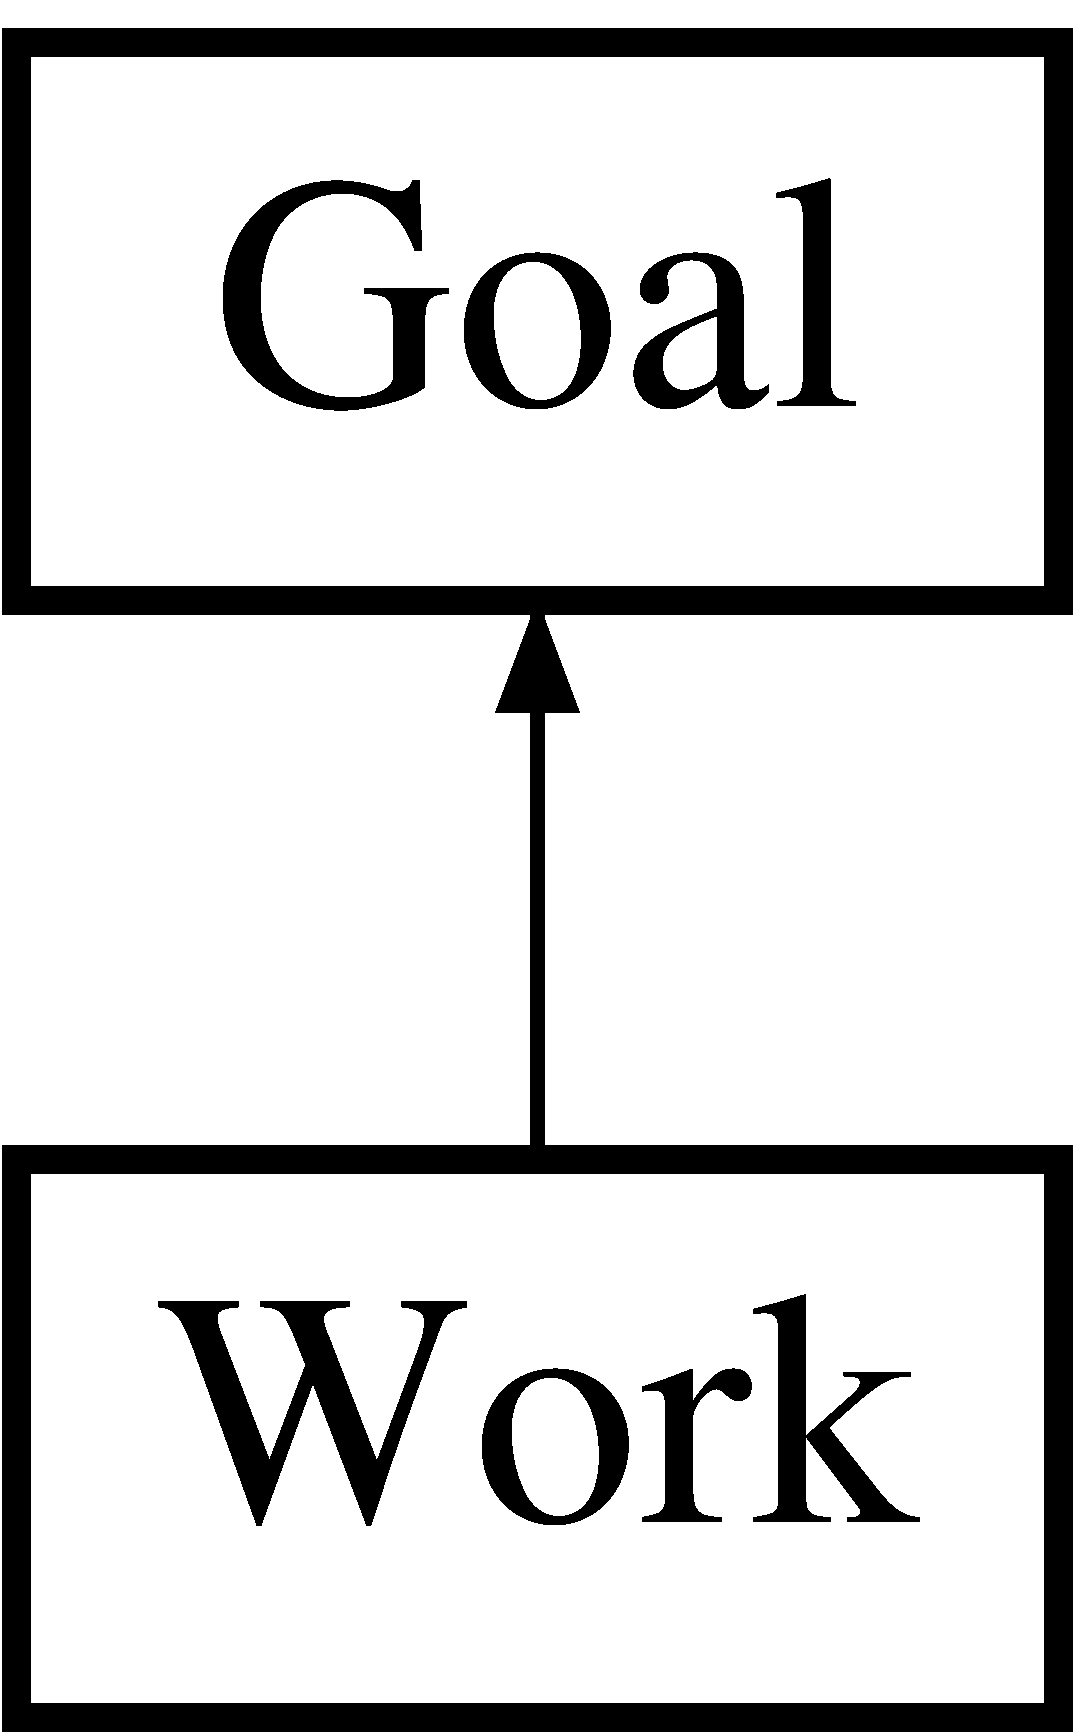
\includegraphics[height=2.000000cm]{class_work}
\end{center}
\end{figure}
\subsection*{Public Member Functions}
\begin{DoxyCompactItemize}
\item 
\hyperlink{class_work_a509eb5062adfa7a18d5afbda644a9f01}{Work} (void)
\begin{DoxyCompactList}\small\item\em Default constructor. \end{DoxyCompactList}\item 
\hyperlink{class_work_a78f0a891f2ae21fb43bc6bbea6c98d64}{$\sim$\-Work} (void)
\begin{DoxyCompactList}\small\item\em Destructor. \end{DoxyCompactList}\item 
bool \hyperlink{class_work_a40c1c9341d1168f04eb4007bb65782aa}{Check\-For\-Trigger} (std\-::map$<$ Enum\-Space\-::\-Need\-Types, int $>$)
\begin{DoxyCompactList}\small\item\em Check for trigger. \end{DoxyCompactList}\item 
std\-::map$<$ Enum\-Space\-::\-Need\-Types, \\*
int $>$ $\ast$ \hyperlink{class_work_a0216999798080e27c939fb9048e4696c}{Modify\-Needs} ()
\begin{DoxyCompactList}\small\item\em Gets the modify needs. \end{DoxyCompactList}\end{DoxyCompactItemize}


\subsection{Detailed Description}
\hyperlink{class_work}{Work}. 

\begin{DoxyAuthor}{Author}
Hamish Carrier 
\end{DoxyAuthor}
\begin{DoxyDate}{Date}
10/11/2013 
\end{DoxyDate}


\subsection{Constructor \& Destructor Documentation}
\hypertarget{class_work_a509eb5062adfa7a18d5afbda644a9f01}{\index{Work@{Work}!Work@{Work}}
\index{Work@{Work}!Work@{Work}}
\subsubsection[{Work}]{\setlength{\rightskip}{0pt plus 5cm}Work\-::\-Work (
\begin{DoxyParamCaption}
\item[{void}]{}
\end{DoxyParamCaption}
)}}\label{class_work_a509eb5062adfa7a18d5afbda644a9f01}


Default constructor. 

\begin{DoxyAuthor}{Author}
Hamish Carrier 
\end{DoxyAuthor}
\begin{DoxyDate}{Date}
10/11/2013 
\end{DoxyDate}
\hypertarget{class_work_a78f0a891f2ae21fb43bc6bbea6c98d64}{\index{Work@{Work}!$\sim$\-Work@{$\sim$\-Work}}
\index{$\sim$\-Work@{$\sim$\-Work}!Work@{Work}}
\subsubsection[{$\sim$\-Work}]{\setlength{\rightskip}{0pt plus 5cm}Work\-::$\sim$\-Work (
\begin{DoxyParamCaption}
\item[{void}]{}
\end{DoxyParamCaption}
)}}\label{class_work_a78f0a891f2ae21fb43bc6bbea6c98d64}


Destructor. 

\begin{DoxyAuthor}{Author}
Hamish Carrier 
\end{DoxyAuthor}
\begin{DoxyDate}{Date}
10/11/2013 
\end{DoxyDate}


\subsection{Member Function Documentation}
\hypertarget{class_work_a40c1c9341d1168f04eb4007bb65782aa}{\index{Work@{Work}!Check\-For\-Trigger@{Check\-For\-Trigger}}
\index{Check\-For\-Trigger@{Check\-For\-Trigger}!Work@{Work}}
\subsubsection[{Check\-For\-Trigger}]{\setlength{\rightskip}{0pt plus 5cm}bool Work\-::\-Check\-For\-Trigger (
\begin{DoxyParamCaption}
\item[{std\-::map$<$ Enum\-Space\-::\-Need\-Types, int $>$}]{}
\end{DoxyParamCaption}
)}}\label{class_work_a40c1c9341d1168f04eb4007bb65782aa}


Check for trigger. 

\begin{DoxyAuthor}{Author}
Hamish Carrier 
\end{DoxyAuthor}
\begin{DoxyDate}{Date}
10/11/2013
\end{DoxyDate}

\begin{DoxyParams}{Parameters}
{\em parameter1} & The first parameter.\\
\hline
\end{DoxyParams}
\begin{DoxyReturn}{Returns}
true if it succeeds, false if it fails. 
\end{DoxyReturn}
\hypertarget{class_work_a0216999798080e27c939fb9048e4696c}{\index{Work@{Work}!Modify\-Needs@{Modify\-Needs}}
\index{Modify\-Needs@{Modify\-Needs}!Work@{Work}}
\subsubsection[{Modify\-Needs}]{\setlength{\rightskip}{0pt plus 5cm}std\-::map$<$ Enum\-Space\-::\-Need\-Types, int $>$ $\ast$ Work\-::\-Modify\-Needs (
\begin{DoxyParamCaption}
{}
\end{DoxyParamCaption}
)}}\label{class_work_a0216999798080e27c939fb9048e4696c}


Gets the modify needs. 

\begin{DoxyAuthor}{Author}
Hamish Carrier 
\end{DoxyAuthor}
\begin{DoxyDate}{Date}
10/11/2013
\end{DoxyDate}
\begin{DoxyReturn}{Returns}
null if it fails, else. 
\end{DoxyReturn}


The documentation for this class was generated from the following files\-:\begin{DoxyCompactItemize}
\item 
A\-:/\-I\-T/\-Git\-Hub/\-I\-C\-T312/source/ogregraphics/\hyperlink{_work_8h}{Work.\-h}\item 
A\-:/\-I\-T/\-Git\-Hub/\-I\-C\-T312/source/ogregraphics/Work.\-cpp\end{DoxyCompactItemize}

\hypertarget{class_world_map}{\section{World\-Map Class Reference}
\label{class_world_map}\index{World\-Map@{World\-Map}}
}


World map a class that implement the grinning lizard A$\ast$.  




{\ttfamily \#include $<$World\-Map.\-h$>$}

Inheritance diagram for World\-Map\-:\begin{figure}[H]
\begin{center}
\leavevmode
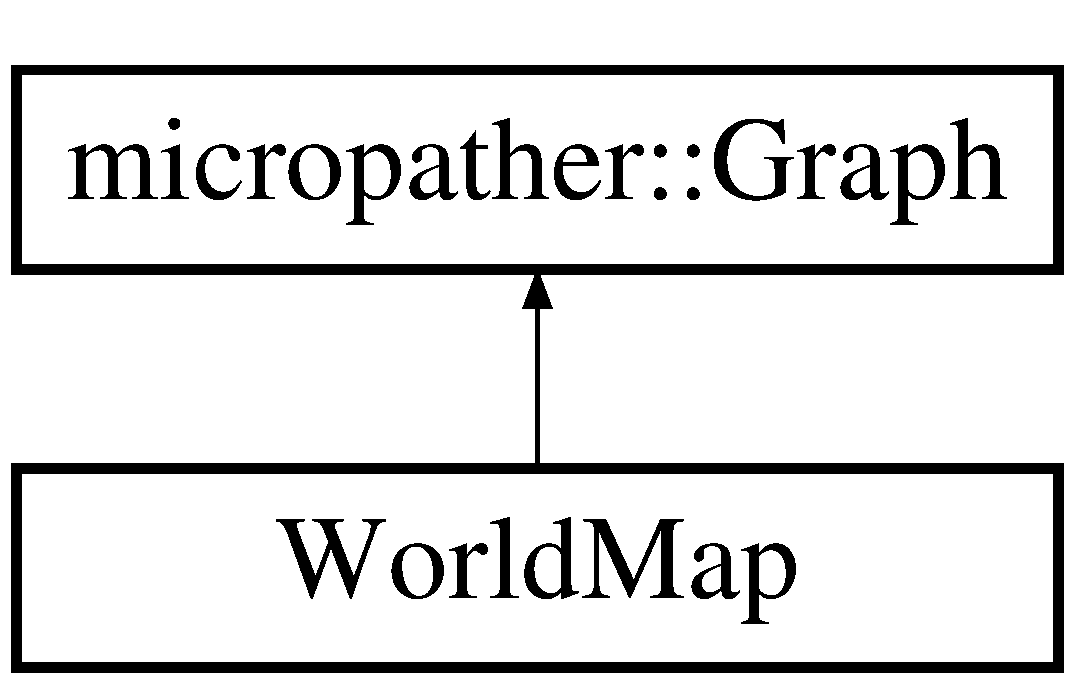
\includegraphics[height=2.000000cm]{class_world_map}
\end{center}
\end{figure}
\subsection*{Public Member Functions}
\begin{DoxyCompactItemize}
\item 
\hyperlink{class_world_map_ad079799989e80b5469c880b8b40e000e}{World\-Map} ()
\begin{DoxyCompactList}\small\item\em Default constructor. \end{DoxyCompactList}\item 
virtual float \hyperlink{class_world_map_a1303b34f21eed11133f8e9895f30121b}{Least\-Cost\-Estimate} (void $\ast$node\-Start, void $\ast$node\-End)
\begin{DoxyCompactList}\small\item\em Least cost estimate. \end{DoxyCompactList}\item 
virtual void \hyperlink{class_world_map_ad82627bde4d4e778f819d2ee9c55bd35}{Adjacent\-Cost} (void $\ast$node, std\-::vector$<$ \hyperlink{structmicropather_1_1_state_cost}{micropather\-::\-State\-Cost} $>$ $\ast$neigbors)
\begin{DoxyCompactList}\small\item\em Adjacent cost. \end{DoxyCompactList}\item 
virtual void \hyperlink{class_world_map_a545c1c031a72cc21ec4c7e9d6103fad7}{Print\-State\-Info} (void $\ast$state)
\begin{DoxyCompactList}\small\item\em Print state information. \end{DoxyCompactList}\item 
bool \hyperlink{class_world_map_afb44a7b557fb1e5ba553ac584f4c1cd3}{Find\-Path} (Ogre\-::\-Vector3 currentpos, Ogre\-::\-Vector3 destination)
\begin{DoxyCompactList}\small\item\em Searches for the best path through the map. \end{DoxyCompactList}\end{DoxyCompactItemize}
\subsection*{Public Attributes}
\begin{DoxyCompactItemize}
\item 
\hypertarget{class_world_map_aea93e909abf8d808f65f8779a49b6b69}{std\-::vector$<$ void $\ast$ $>$ \hyperlink{class_world_map_aea93e909abf8d808f65f8779a49b6b69}{path}}\label{class_world_map_aea93e909abf8d808f65f8779a49b6b69}

\begin{DoxyCompactList}\small\item\em The list of nodes that make up the path. \end{DoxyCompactList}\end{DoxyCompactItemize}


\subsection{Detailed Description}
World map a class that implement the grinning lizard A$\ast$. 

\begin{DoxyAuthor}{Author}
Arran Ford 
\end{DoxyAuthor}
\begin{DoxyDate}{Date}
09/11/2013 
\end{DoxyDate}


\subsection{Constructor \& Destructor Documentation}
\hypertarget{class_world_map_ad079799989e80b5469c880b8b40e000e}{\index{World\-Map@{World\-Map}!World\-Map@{World\-Map}}
\index{World\-Map@{World\-Map}!WorldMap@{World\-Map}}
\subsubsection[{World\-Map}]{\setlength{\rightskip}{0pt plus 5cm}World\-Map\-::\-World\-Map (
\begin{DoxyParamCaption}
{}
\end{DoxyParamCaption}
)}}\label{class_world_map_ad079799989e80b5469c880b8b40e000e}


Default constructor. 

\begin{DoxyAuthor}{Author}
Arran Ford 
\end{DoxyAuthor}
\begin{DoxyDate}{Date}
09/11/2013 
\end{DoxyDate}


\subsection{Member Function Documentation}
\hypertarget{class_world_map_ad82627bde4d4e778f819d2ee9c55bd35}{\index{World\-Map@{World\-Map}!Adjacent\-Cost@{Adjacent\-Cost}}
\index{Adjacent\-Cost@{Adjacent\-Cost}!WorldMap@{World\-Map}}
\subsubsection[{Adjacent\-Cost}]{\setlength{\rightskip}{0pt plus 5cm}void World\-Map\-::\-Adjacent\-Cost (
\begin{DoxyParamCaption}
\item[{void $\ast$}]{node, }
\item[{std\-::vector$<$ {\bf micropather\-::\-State\-Cost} $>$ $\ast$}]{neigbors}
\end{DoxyParamCaption}
)\hspace{0.3cm}{\ttfamily [virtual]}}}\label{class_world_map_ad82627bde4d4e778f819d2ee9c55bd35}


Adjacent cost. 

\begin{DoxyAuthor}{Author}
Arran Ford 
\end{DoxyAuthor}
\begin{DoxyDate}{Date}
09/11/2013
\end{DoxyDate}

\begin{DoxyParams}[1]{Parameters}
\mbox{\tt in,out}  & {\em node} & If non-\/null, the node. \\
\hline
\mbox{\tt in,out}  & {\em neigbors} & If non-\/null, the neigbors. \\
\hline
\end{DoxyParams}
\hypertarget{class_world_map_afb44a7b557fb1e5ba553ac584f4c1cd3}{\index{World\-Map@{World\-Map}!Find\-Path@{Find\-Path}}
\index{Find\-Path@{Find\-Path}!WorldMap@{World\-Map}}
\subsubsection[{Find\-Path}]{\setlength{\rightskip}{0pt plus 5cm}bool World\-Map\-::\-Find\-Path (
\begin{DoxyParamCaption}
\item[{Ogre\-::\-Vector3}]{currentpos, }
\item[{Ogre\-::\-Vector3}]{destination}
\end{DoxyParamCaption}
)}}\label{class_world_map_afb44a7b557fb1e5ba553ac584f4c1cd3}


Searches for the best path through the map. 

\begin{DoxyAuthor}{Author}
Arran Ford 
\end{DoxyAuthor}
\begin{DoxyDate}{Date}
09/11/2013
\end{DoxyDate}

\begin{DoxyParams}{Parameters}
{\em currentpos} & The currentpos. \\
\hline
{\em destination} & Destination for the.\\
\hline
\end{DoxyParams}
\begin{DoxyReturn}{Returns}
true if it succeeds, false if it fails. 
\end{DoxyReturn}
\hypertarget{class_world_map_a1303b34f21eed11133f8e9895f30121b}{\index{World\-Map@{World\-Map}!Least\-Cost\-Estimate@{Least\-Cost\-Estimate}}
\index{Least\-Cost\-Estimate@{Least\-Cost\-Estimate}!WorldMap@{World\-Map}}
\subsubsection[{Least\-Cost\-Estimate}]{\setlength{\rightskip}{0pt plus 5cm}float World\-Map\-::\-Least\-Cost\-Estimate (
\begin{DoxyParamCaption}
\item[{void $\ast$}]{node\-Start, }
\item[{void $\ast$}]{node\-End}
\end{DoxyParamCaption}
)\hspace{0.3cm}{\ttfamily [virtual]}}}\label{class_world_map_a1303b34f21eed11133f8e9895f30121b}


Least cost estimate. 

\begin{DoxyAuthor}{Author}
Arran Ford 
\end{DoxyAuthor}
\begin{DoxyDate}{Date}
09/11/2013
\end{DoxyDate}

\begin{DoxyParams}[1]{Parameters}
\mbox{\tt in,out}  & {\em node\-Start} & If non-\/null, the node start. \\
\hline
\mbox{\tt in,out}  & {\em node\-End} & If non-\/null, the node end.\\
\hline
\end{DoxyParams}
\begin{DoxyReturn}{Returns}
. 
\end{DoxyReturn}


Implements \hyperlink{classmicropather_1_1_graph_a7a284a95607553e15439ecc7a1440abc}{micropather\-::\-Graph}.

\hypertarget{class_world_map_a545c1c031a72cc21ec4c7e9d6103fad7}{\index{World\-Map@{World\-Map}!Print\-State\-Info@{Print\-State\-Info}}
\index{Print\-State\-Info@{Print\-State\-Info}!WorldMap@{World\-Map}}
\subsubsection[{Print\-State\-Info}]{\setlength{\rightskip}{0pt plus 5cm}void World\-Map\-::\-Print\-State\-Info (
\begin{DoxyParamCaption}
\item[{void $\ast$}]{state}
\end{DoxyParamCaption}
)\hspace{0.3cm}{\ttfamily [virtual]}}}\label{class_world_map_a545c1c031a72cc21ec4c7e9d6103fad7}


Print state information. 

\begin{DoxyAuthor}{Author}
Arran Ford 
\end{DoxyAuthor}
\begin{DoxyDate}{Date}
09/11/2013
\end{DoxyDate}

\begin{DoxyParams}[1]{Parameters}
\mbox{\tt in,out}  & {\em state} & If non-\/null, the state. \\
\hline
\end{DoxyParams}


Implements \hyperlink{classmicropather_1_1_graph_a9ca57ce2dceccece9654545b7dfad6ff}{micropather\-::\-Graph}.



The documentation for this class was generated from the following files\-:\begin{DoxyCompactItemize}
\item 
A\-:/\-I\-T/\-Git\-Hub/\-I\-C\-T312/source/ogregraphics/\hyperlink{_world_map_8h}{World\-Map.\-h}\item 
A\-:/\-I\-T/\-Git\-Hub/\-I\-C\-T312/source/ogregraphics/World\-Map.\-cpp\end{DoxyCompactItemize}

\chapter{File Documentation}
\hypertarget{_action_manager_8h}{\section{A\-:/\-I\-T/\-Git\-Hub/\-I\-C\-T312/source/ogregraphics/\-Action\-Manager.h File Reference}
\label{_action_manager_8h}\index{A\-:/\-I\-T/\-Git\-Hub/\-I\-C\-T312/source/ogregraphics/\-Action\-Manager.\-h@{A\-:/\-I\-T/\-Git\-Hub/\-I\-C\-T312/source/ogregraphics/\-Action\-Manager.\-h}}
}


Declares the action manager class.  


{\ttfamily \#include \char`\"{}stdafx.\-h\char`\"{}}\\*
{\ttfamily \#include \char`\"{}Action.\-h\char`\"{}}\\*
{\ttfamily \#include \char`\"{}Sit.\-h\char`\"{}}\\*
{\ttfamily \#include \char`\"{}Use\-Computer.\-h\char`\"{}}\\*
{\ttfamily \#include \char`\"{}Emotion\-Manager.\-h\char`\"{}}\\*
\subsection*{Classes}
\begin{DoxyCompactItemize}
\item 
class \hyperlink{class_action_manager}{Action\-Manager}
\begin{DoxyCompactList}\small\item\em Manager for actions. \end{DoxyCompactList}\end{DoxyCompactItemize}


\subsection{Detailed Description}
Declares the action manager class. 
\hypertarget{_bad_8h}{\section{A\-:/\-I\-T/\-Git\-Hub/\-I\-C\-T312/source/ogregraphics/\-Bad.h File Reference}
\label{_bad_8h}\index{A\-:/\-I\-T/\-Git\-Hub/\-I\-C\-T312/source/ogregraphics/\-Bad.\-h@{A\-:/\-I\-T/\-Git\-Hub/\-I\-C\-T312/source/ogregraphics/\-Bad.\-h}}
}


Declares the bad class.  


{\ttfamily \#include \char`\"{}mood.\-h\char`\"{}}\\*
\subsection*{Classes}
\begin{DoxyCompactItemize}
\item 
class \hyperlink{class_bad}{Bad}
\begin{DoxyCompactList}\small\item\em \hyperlink{class_bad}{Bad}. \end{DoxyCompactList}\end{DoxyCompactItemize}


\subsection{Detailed Description}
Declares the bad class. 
\hypertarget{_collision_object_8h}{\section{A\-:/\-I\-T/\-Git\-Hub/\-I\-C\-T312/source/ogregraphics/\-Collision\-Object.h File Reference}
\label{_collision_object_8h}\index{A\-:/\-I\-T/\-Git\-Hub/\-I\-C\-T312/source/ogregraphics/\-Collision\-Object.\-h@{A\-:/\-I\-T/\-Git\-Hub/\-I\-C\-T312/source/ogregraphics/\-Collision\-Object.\-h}}
}


Declares the collision object class.  


{\ttfamily \#include \char`\"{}Collision\-World\-Singleton.\-h\char`\"{}}\\*
{\ttfamily \#include \char`\"{}Ogre\-Bullet\-Collisions\-Pre\-Requisites.\-h\char`\"{}}\\*
{\ttfamily \#include \char`\"{}Ogre\-Bullet\-Collisions\-World.\-h\char`\"{}}\\*
{\ttfamily \#include \char`\"{}Ogre\-Bullet\-Collisions.\-h\char`\"{}}\\*
{\ttfamily \#include \char`\"{}Ogre\-Bullet\-Collisions\-Object.\-h\char`\"{}}\\*
{\ttfamily \#include \char`\"{}Debug/\-Ogre\-Bullet\-Collisions\-Debug\-Shape.\-h\char`\"{}}\\*
{\ttfamily \#include \char`\"{}Ogre\-Bullet\-Collisions\-Object\-State.\-h\char`\"{}}\\*
{\ttfamily \#include \char`\"{}Ogre\-Bullet\-Collisions\-Shape.\-h\char`\"{}}\\*
{\ttfamily \#include \char`\"{}Vector3.\-h\char`\"{}}\\*
{\ttfamily \#include \char`\"{}I\-Object.\-h\char`\"{}}\\*
\subsection*{Classes}
\begin{DoxyCompactItemize}
\item 
class \hyperlink{class_collision_object}{Collision\-Object}
\begin{DoxyCompactList}\small\item\em Collision object. \end{DoxyCompactList}\end{DoxyCompactItemize}


\subsection{Detailed Description}
Declares the collision object class. 
\hypertarget{_contact_8h}{\section{A\-:/\-I\-T/\-Git\-Hub/\-I\-C\-T312/source/ogregraphics/\-Contact.h File Reference}
\label{_contact_8h}\index{A\-:/\-I\-T/\-Git\-Hub/\-I\-C\-T312/source/ogregraphics/\-Contact.\-h@{A\-:/\-I\-T/\-Git\-Hub/\-I\-C\-T312/source/ogregraphics/\-Contact.\-h}}
}


Declares the contact class.  


{\ttfamily \#include $<$cmath$>$}\\*
{\ttfamily \#include \char`\"{}Rigid\-Body\-Object.\-h\char`\"{}}\\*
\subsection*{Classes}
\begin{DoxyCompactItemize}
\item 
struct \hyperlink{struct_physics_1_1_contact}{Physics\-::\-Contact}
\begin{DoxyCompactList}\small\item\em \hyperlink{struct_physics_1_1_contact}{Contact}. \end{DoxyCompactList}\end{DoxyCompactItemize}


\subsection{Detailed Description}
Declares the contact class. 
\hypertarget{_debug_drawer_og_8h}{\section{A\-:/\-I\-T/\-Git\-Hub/\-I\-C\-T312/source/ogregraphics/\-Debug\-Drawer\-Og.h File Reference}
\label{_debug_drawer_og_8h}\index{A\-:/\-I\-T/\-Git\-Hub/\-I\-C\-T312/source/ogregraphics/\-Debug\-Drawer\-Og.\-h@{A\-:/\-I\-T/\-Git\-Hub/\-I\-C\-T312/source/ogregraphics/\-Debug\-Drawer\-Og.\-h}}
}


An implementation of the Bullet debug drawer taken from the Ogre Wiki \href{http://www.ogre3d.org/tikiwiki/BulletDebugDrawer&structure=Cookbook}{\tt http\-://www.\-ogre3d.\-org/tikiwiki/\-Bullet\-Debug\-Drawer\&structure=\-Cookbook}.  


{\ttfamily \#include \char`\"{}Collision\-World\-Singleton.\-h\char`\"{}}\\*
{\ttfamily \#include \char`\"{}boost\textbackslash{}range\textbackslash{}detail\textbackslash{}common.\-hpp\char`\"{}}\\*
\subsection*{Classes}
\begin{DoxyCompactItemize}
\item 
class \hyperlink{class_ogre_debug_drawer}{Ogre\-Debug\-Drawer}
\end{DoxyCompactItemize}
\subsection*{Macros}
\begin{DoxyCompactItemize}
\item 
\#define \hyperlink{_debug_drawer_og_8h_ae73110856f2f37d62cc9b37f04fafdb4}{Debug\-Drawer\-\_\-h\-\_\-\-\_\-}
\begin{DoxyCompactList}\small\item\em A macro that defines debug drawer h. \end{DoxyCompactList}\end{DoxyCompactItemize}


\subsection{Detailed Description}
An implementation of the Bullet debug drawer taken from the Ogre Wiki \href{http://www.ogre3d.org/tikiwiki/BulletDebugDrawer&structure=Cookbook}{\tt http\-://www.\-ogre3d.\-org/tikiwiki/\-Bullet\-Debug\-Drawer\&structure=\-Cookbook}. 

\subsection{Macro Definition Documentation}
\hypertarget{_debug_drawer_og_8h_ae73110856f2f37d62cc9b37f04fafdb4}{\index{Debug\-Drawer\-Og.\-h@{Debug\-Drawer\-Og.\-h}!Debug\-Drawer\-\_\-h\-\_\-\-\_\-@{Debug\-Drawer\-\_\-h\-\_\-\-\_\-}}
\index{Debug\-Drawer\-\_\-h\-\_\-\-\_\-@{Debug\-Drawer\-\_\-h\-\_\-\-\_\-}!DebugDrawerOg.h@{Debug\-Drawer\-Og.\-h}}
\subsubsection[{Debug\-Drawer\-\_\-h\-\_\-\-\_\-}]{\setlength{\rightskip}{0pt plus 5cm}\#define Debug\-Drawer\-\_\-h\-\_\-\-\_\-}}\label{_debug_drawer_og_8h_ae73110856f2f37d62cc9b37f04fafdb4}


A macro that defines debug drawer h. 

\begin{DoxyAuthor}{Author}
Ogre Wiki 
\end{DoxyAuthor}
\begin{DoxyDate}{Date}
31/10/2013 
\end{DoxyDate}

\hypertarget{_easy_going_8h}{\section{A\-:/\-I\-T/\-Git\-Hub/\-I\-C\-T312/source/ogregraphics/\-Easy\-Going.h File Reference}
\label{_easy_going_8h}\index{A\-:/\-I\-T/\-Git\-Hub/\-I\-C\-T312/source/ogregraphics/\-Easy\-Going.\-h@{A\-:/\-I\-T/\-Git\-Hub/\-I\-C\-T312/source/ogregraphics/\-Easy\-Going.\-h}}
}


Declares the easy going class.  


{\ttfamily \#include \char`\"{}stdafx.\-h\char`\"{}}\\*
{\ttfamily \#include \char`\"{}Trait.\-h\char`\"{}}\\*
\subsection*{Classes}
\begin{DoxyCompactItemize}
\item 
class \hyperlink{class_easy_going}{Easy\-Going}
\begin{DoxyCompactList}\small\item\em Easy going. \end{DoxyCompactList}\end{DoxyCompactItemize}


\subsection{Detailed Description}
Declares the easy going class. 
\hypertarget{_emotion_8h}{\section{A\-:/\-I\-T/\-Git\-Hub/\-I\-C\-T312/source/ogregraphics/\-Emotion.h File Reference}
\label{_emotion_8h}\index{A\-:/\-I\-T/\-Git\-Hub/\-I\-C\-T312/source/ogregraphics/\-Emotion.\-h@{A\-:/\-I\-T/\-Git\-Hub/\-I\-C\-T312/source/ogregraphics/\-Emotion.\-h}}
}


Declares the emotion class.  


{\ttfamily \#include \char`\"{}stdafx.\-h\char`\"{}}\\*
{\ttfamily \#include \char`\"{}Enum\-Space.\-h\char`\"{}}\\*
\subsection*{Classes}
\begin{DoxyCompactItemize}
\item 
class \hyperlink{classabstract}{abstract}
\end{DoxyCompactItemize}


\subsection{Detailed Description}
Declares the emotion class. 
\hypertarget{_emotion_manager_8h}{\section{A\-:/\-I\-T/\-Git\-Hub/\-I\-C\-T312/source/ogregraphics/\-Emotion\-Manager.h File Reference}
\label{_emotion_manager_8h}\index{A\-:/\-I\-T/\-Git\-Hub/\-I\-C\-T312/source/ogregraphics/\-Emotion\-Manager.\-h@{A\-:/\-I\-T/\-Git\-Hub/\-I\-C\-T312/source/ogregraphics/\-Emotion\-Manager.\-h}}
}


Declares the emotion manager class.  


{\ttfamily \#include \char`\"{}stdafx.\-h\char`\"{}}\\*
{\ttfamily \#include \char`\"{}Emotion.\-h\char`\"{}}\\*
{\ttfamily \#include \char`\"{}Happy.\-h\char`\"{}}\\*
{\ttfamily \#include \char`\"{}Sad.\-h\char`\"{}}\\*
{\ttfamily \#include \char`\"{}Neutral.\-h\char`\"{}}\\*
{\ttfamily \#include \char`\"{}Enum\-Space.\-h\char`\"{}}\\*
\subsection*{Classes}
\begin{DoxyCompactItemize}
\item 
class \hyperlink{class_emotion_manager}{Emotion\-Manager}
\begin{DoxyCompactList}\small\item\em Manager for emotions. \end{DoxyCompactList}\end{DoxyCompactItemize}


\subsection{Detailed Description}
Declares the emotion manager class. 
\hypertarget{_enum_space_8h}{\section{A\-:/\-I\-T/\-Git\-Hub/\-I\-C\-T312/source/ogregraphics/\-Enum\-Space.h File Reference}
\label{_enum_space_8h}\index{A\-:/\-I\-T/\-Git\-Hub/\-I\-C\-T312/source/ogregraphics/\-Enum\-Space.\-h@{A\-:/\-I\-T/\-Git\-Hub/\-I\-C\-T312/source/ogregraphics/\-Enum\-Space.\-h}}
}


Declares the enum space class.  


{\ttfamily \#include \char`\"{}stdafx.\-h\char`\"{}}\\*
\subsection*{Enumerations}
\begin{DoxyCompactItemize}
\item 
enum {\bfseries Action\-Types} \{ {\bfseries enum\-Sit}, 
{\bfseries enum\-Use\-Computer}, 
{\bfseries Action\-Types\-\_\-\-Max} = enum\-Use\-Computer
 \}
\begin{DoxyCompactList}\small\item\em Values that represent Action\-Types. \end{DoxyCompactList}\item 
enum {\bfseries Mood\-Types} \{ {\bfseries enum\-Good}, 
{\bfseries enum\-Bad}, 
{\bfseries Mood\-Types\-\_\-\-Max} = enum\-Bad
 \}
\begin{DoxyCompactList}\small\item\em Values that represent Mood\-Types. \end{DoxyCompactList}\item 
enum {\bfseries Emotion\-Types} \{ {\bfseries enum\-Neutral}, 
{\bfseries enum\-Happy}, 
{\bfseries enum\-Sad}, 
{\bfseries Emotion\-Types\-\_\-\-Max} = enum\-Sad
 \}
\begin{DoxyCompactList}\small\item\em Values that represent Emotion\-Types. \end{DoxyCompactList}\item 
enum {\bfseries Need\-Types} \{ {\bfseries enum\-Grades}, 
{\bfseries enum\-Comfort}, 
{\bfseries enum\-Fun}, 
{\bfseries Need\-Types\-\_\-\-Max} = enum\-Fun
 \}
\begin{DoxyCompactList}\small\item\em Values that represent Need\-Types. \end{DoxyCompactList}\item 
enum {\bfseries N\-P\-C\-State} \{ \\*
{\bfseries enum\-Searching}, 
{\bfseries enum\-Idling}, 
{\bfseries enum\-Interacting}, 
{\bfseries enum\-Thinking}, 
\\*
{\bfseries N\-P\-C\-State\-\_\-\-Max} = enum\-Thinking
 \}
\begin{DoxyCompactList}\small\item\em Values that represent N\-P\-C\-State. \end{DoxyCompactList}\end{DoxyCompactItemize}


\subsection{Detailed Description}
Declares the enum space class. 
\hypertarget{_frame_listener_8h}{\section{A\-:/\-I\-T/\-Git\-Hub/\-I\-C\-T312/source/ogregraphics/\-Frame\-Listener.h File Reference}
\label{_frame_listener_8h}\index{A\-:/\-I\-T/\-Git\-Hub/\-I\-C\-T312/source/ogregraphics/\-Frame\-Listener.\-h@{A\-:/\-I\-T/\-Git\-Hub/\-I\-C\-T312/source/ogregraphics/\-Frame\-Listener.\-h}}
}


Declares the frame listener class.  


{\ttfamily \#include \char`\"{}Debug\-Drawer.\-h\char`\"{}}\\*
\subsection*{Classes}
\begin{DoxyCompactItemize}
\item 
class \hyperlink{class_graphics_1_1_frame_listener}{Graphics\-::\-Frame\-Listener}
\begin{DoxyCompactList}\small\item\em Frame listener. \end{DoxyCompactList}\end{DoxyCompactItemize}


\subsection{Detailed Description}
Declares the frame listener class. 
\hypertarget{_fun_loving_8h}{\section{A\-:/\-I\-T/\-Git\-Hub/\-I\-C\-T312/source/ogregraphics/\-Fun\-Loving.h File Reference}
\label{_fun_loving_8h}\index{A\-:/\-I\-T/\-Git\-Hub/\-I\-C\-T312/source/ogregraphics/\-Fun\-Loving.\-h@{A\-:/\-I\-T/\-Git\-Hub/\-I\-C\-T312/source/ogregraphics/\-Fun\-Loving.\-h}}
}


Declares the fun loving class.  


{\ttfamily \#include \char`\"{}Trait.\-h\char`\"{}}\\*
\subsection*{Classes}
\begin{DoxyCompactItemize}
\item 
class \hyperlink{class_fun_loving}{Fun\-Loving}
\begin{DoxyCompactList}\small\item\em Fun loving. \end{DoxyCompactList}\end{DoxyCompactItemize}


\subsection{Detailed Description}
Declares the fun loving class. 
\hypertarget{_generic_object_8h}{\section{A\-:/\-I\-T/\-Git\-Hub/\-I\-C\-T312/source/ogregraphics/\-Generic\-Object.h File Reference}
\label{_generic_object_8h}\index{A\-:/\-I\-T/\-Git\-Hub/\-I\-C\-T312/source/ogregraphics/\-Generic\-Object.\-h@{A\-:/\-I\-T/\-Git\-Hub/\-I\-C\-T312/source/ogregraphics/\-Generic\-Object.\-h}}
}


Declares the generic object class.  


{\ttfamily \#include \char`\"{}I\-Object.\-h\char`\"{}}\\*
\subsection*{Classes}
\begin{DoxyCompactItemize}
\item 
class \hyperlink{class_objects_1_1_generic_object}{Objects\-::\-Generic\-Object}
\begin{DoxyCompactList}\small\item\em Generic object. \end{DoxyCompactList}\end{DoxyCompactItemize}


\subsection{Detailed Description}
Declares the generic object class. 
\hypertarget{_goal_8h}{\section{A\-:/\-I\-T/\-Git\-Hub/\-I\-C\-T312/source/ogregraphics/\-Goal.h File Reference}
\label{_goal_8h}\index{A\-:/\-I\-T/\-Git\-Hub/\-I\-C\-T312/source/ogregraphics/\-Goal.\-h@{A\-:/\-I\-T/\-Git\-Hub/\-I\-C\-T312/source/ogregraphics/\-Goal.\-h}}
}


Declares the goal class.  


{\ttfamily \#include \char`\"{}stdafx.\-h\char`\"{}}\\*
{\ttfamily \#include \char`\"{}Action.\-h\char`\"{}}\\*
{\ttfamily \#include \char`\"{}Enum\-Space.\-h\char`\"{}}\\*
{\ttfamily \#include \char`\"{}Action\-Manager.\-h\char`\"{}}\\*
\subsection*{Classes}
\begin{DoxyCompactItemize}
\item 
class \hyperlink{classabstract}{abstract}
\end{DoxyCompactItemize}


\subsection{Detailed Description}
Declares the goal class. 
\hypertarget{_good_8h}{\section{A\-:/\-I\-T/\-Git\-Hub/\-I\-C\-T312/source/ogregraphics/\-Good.h File Reference}
\label{_good_8h}\index{A\-:/\-I\-T/\-Git\-Hub/\-I\-C\-T312/source/ogregraphics/\-Good.\-h@{A\-:/\-I\-T/\-Git\-Hub/\-I\-C\-T312/source/ogregraphics/\-Good.\-h}}
}


Declares the good class.  


{\ttfamily \#include \char`\"{}mood.\-h\char`\"{}}\\*
\subsection*{Classes}
\begin{DoxyCompactItemize}
\item 
class \hyperlink{class_good}{Good}
\begin{DoxyCompactList}\small\item\em \hyperlink{class_good}{Good}. \end{DoxyCompactList}\end{DoxyCompactItemize}


\subsection{Detailed Description}
Declares the good class. 
\hypertarget{_happy_8h}{\section{A\-:/\-I\-T/\-Git\-Hub/\-I\-C\-T312/source/ogregraphics/\-Happy.h File Reference}
\label{_happy_8h}\index{A\-:/\-I\-T/\-Git\-Hub/\-I\-C\-T312/source/ogregraphics/\-Happy.\-h@{A\-:/\-I\-T/\-Git\-Hub/\-I\-C\-T312/source/ogregraphics/\-Happy.\-h}}
}


Declares the happy class.  


{\ttfamily \#include \char`\"{}emotion.\-h\char`\"{}}\\*
\subsection*{Classes}
\begin{DoxyCompactItemize}
\item 
class \hyperlink{class_happy}{Happy}
\begin{DoxyCompactList}\small\item\em \hyperlink{class_happy}{Happy}. \end{DoxyCompactList}\end{DoxyCompactItemize}


\subsection{Detailed Description}
Declares the happy class. 
\hypertarget{_i_object_8h}{\section{A\-:/\-I\-T/\-Git\-Hub/\-I\-C\-T312/source/ogregraphics/\-I\-Object.h File Reference}
\label{_i_object_8h}\index{A\-:/\-I\-T/\-Git\-Hub/\-I\-C\-T312/source/ogregraphics/\-I\-Object.\-h@{A\-:/\-I\-T/\-Git\-Hub/\-I\-C\-T312/source/ogregraphics/\-I\-Object.\-h}}
}


Declares the I\-Object interface.  


{\ttfamily \#include \char`\"{}Collision\-Object.\-h\char`\"{}}\\*
\subsection*{Classes}
\begin{DoxyCompactItemize}
\item 
class \hyperlink{class_objects_1_1_i_object}{Objects\-::\-I\-Object}
\begin{DoxyCompactList}\small\item\em Object. \end{DoxyCompactList}\end{DoxyCompactItemize}


\subsection{Detailed Description}
Declares the I\-Object interface. 
\hypertarget{_i_t_building_scene_8h}{\section{A\-:/\-I\-T/\-Git\-Hub/\-I\-C\-T312/source/ogregraphics/\-I\-T\-Building\-Scene.h File Reference}
\label{_i_t_building_scene_8h}\index{A\-:/\-I\-T/\-Git\-Hub/\-I\-C\-T312/source/ogregraphics/\-I\-T\-Building\-Scene.\-h@{A\-:/\-I\-T/\-Git\-Hub/\-I\-C\-T312/source/ogregraphics/\-I\-T\-Building\-Scene.\-h}}
}


Declares the iterator building scene class.  


{\ttfamily \#include \char`\"{}I\-Scene.\-h\char`\"{}}\\*
{\ttfamily \#include \char`\"{}Exit\-Scene.\-h\char`\"{}}\\*
{\ttfamily \#include \char`\"{}Scene\-Loader.\-h\char`\"{}}\\*
{\ttfamily \#include \char`\"{}Target\-Object.\-h\char`\"{}}\\*
{\ttfamily \#include \char`\"{}Projectile\-Object.\-h\char`\"{}}\\*
\subsection*{Classes}
\begin{DoxyCompactItemize}
\item 
class \hyperlink{class_scenes_1_1_i_t_building_scene}{Scenes\-::\-I\-T\-Building\-Scene}
\begin{DoxyCompactList}\small\item\em Iterator building scene. \end{DoxyCompactList}\end{DoxyCompactItemize}
\subsection*{Namespaces}
\begin{DoxyCompactItemize}
\item 
\hyperlink{namespace_scenes}{Scenes}
\begin{DoxyCompactList}\small\item\em \end{DoxyCompactList}\end{DoxyCompactItemize}
\subsection*{Constant Groups}
\begin{DoxyCompactItemize}
\item 
\hyperlink{namespace_scenes}{Scenes}
\begin{DoxyCompactList}\small\item\em \end{DoxyCompactList}\end{DoxyCompactItemize}


\subsection{Detailed Description}
Declares the iterator building scene class. 
\hypertarget{_map_node_8h}{\section{A\-:/\-I\-T/\-Git\-Hub/\-I\-C\-T312/source/ogregraphics/\-Map\-Node.h File Reference}
\label{_map_node_8h}\index{A\-:/\-I\-T/\-Git\-Hub/\-I\-C\-T312/source/ogregraphics/\-Map\-Node.\-h@{A\-:/\-I\-T/\-Git\-Hub/\-I\-C\-T312/source/ogregraphics/\-Map\-Node.\-h}}
}


Declares the map node class.  


{\ttfamily \#include \char`\"{}Vector3.\-h\char`\"{}}\\*
\subsection*{Classes}
\begin{DoxyCompactItemize}
\item 
class \hyperlink{class_map_node}{Map\-Node}
\begin{DoxyCompactList}\small\item\em This class is a node that can be moved to in the path finding. \end{DoxyCompactList}\end{DoxyCompactItemize}


\subsection{Detailed Description}
Declares the map node class. 
\hypertarget{_mood_8h}{\section{A\-:/\-I\-T/\-Git\-Hub/\-I\-C\-T312/source/ogregraphics/\-Mood.h File Reference}
\label{_mood_8h}\index{A\-:/\-I\-T/\-Git\-Hub/\-I\-C\-T312/source/ogregraphics/\-Mood.\-h@{A\-:/\-I\-T/\-Git\-Hub/\-I\-C\-T312/source/ogregraphics/\-Mood.\-h}}
}


Declares the mood class.  


{\ttfamily \#include \char`\"{}stdafx.\-h\char`\"{}}\\*
{\ttfamily \#include \char`\"{}Enum\-Space.\-h\char`\"{}}\\*
\subsection*{Classes}
\begin{DoxyCompactItemize}
\item 
class \hyperlink{classabstract}{abstract}
\end{DoxyCompactItemize}


\subsection{Detailed Description}
Declares the mood class. 
\hypertarget{_mood_manager_8h}{\section{A\-:/\-I\-T/\-Git\-Hub/\-I\-C\-T312/source/ogregraphics/\-Mood\-Manager.h File Reference}
\label{_mood_manager_8h}\index{A\-:/\-I\-T/\-Git\-Hub/\-I\-C\-T312/source/ogregraphics/\-Mood\-Manager.\-h@{A\-:/\-I\-T/\-Git\-Hub/\-I\-C\-T312/source/ogregraphics/\-Mood\-Manager.\-h}}
}


Declares the mood manager class.  


{\ttfamily \#include \char`\"{}stdafx.\-h\char`\"{}}\\*
{\ttfamily \#include \char`\"{}Mood.\-h\char`\"{}}\\*
{\ttfamily \#include \char`\"{}Good.\-h\char`\"{}}\\*
{\ttfamily \#include \char`\"{}Bad.\-h\char`\"{}}\\*
{\ttfamily \#include \char`\"{}Emotion\-Manager.\-h\char`\"{}}\\*
\subsection*{Classes}
\begin{DoxyCompactItemize}
\item 
class \hyperlink{class_mood_manager}{Mood\-Manager}
\begin{DoxyCompactList}\small\item\em Manager for moods. \end{DoxyCompactList}\end{DoxyCompactItemize}


\subsection{Detailed Description}
Declares the mood manager class. 
\hypertarget{_move_item_8h}{\section{A\-:/\-I\-T/\-Git\-Hub/\-I\-C\-T312/source/ogregraphics/\-Move\-Item.h File Reference}
\label{_move_item_8h}\index{A\-:/\-I\-T/\-Git\-Hub/\-I\-C\-T312/source/ogregraphics/\-Move\-Item.\-h@{A\-:/\-I\-T/\-Git\-Hub/\-I\-C\-T312/source/ogregraphics/\-Move\-Item.\-h}}
}


Declares the move item class.  


{\ttfamily \#include \char`\"{}stdafx.\-h\char`\"{}}\\*
{\ttfamily \#include \char`\"{}Action.\-h\char`\"{}}\\*
\subsection*{Classes}
\begin{DoxyCompactItemize}
\item 
class \hyperlink{class_move_item}{Move\-Item}
\begin{DoxyCompactList}\small\item\em Move item. \end{DoxyCompactList}\end{DoxyCompactItemize}


\subsection{Detailed Description}
Declares the move item class. 
\hypertarget{_neutral_8h}{\section{A\-:/\-I\-T/\-Git\-Hub/\-I\-C\-T312/source/ogregraphics/\-Neutral.h File Reference}
\label{_neutral_8h}\index{A\-:/\-I\-T/\-Git\-Hub/\-I\-C\-T312/source/ogregraphics/\-Neutral.\-h@{A\-:/\-I\-T/\-Git\-Hub/\-I\-C\-T312/source/ogregraphics/\-Neutral.\-h}}
}


Declares the neutral class.  


{\ttfamily \#include \char`\"{}emotion.\-h\char`\"{}}\\*
\subsection*{Classes}
\begin{DoxyCompactItemize}
\item 
class \hyperlink{class_neutral}{Neutral}
\begin{DoxyCompactList}\small\item\em \hyperlink{class_neutral}{Neutral}. \end{DoxyCompactList}\end{DoxyCompactItemize}


\subsection{Detailed Description}
Declares the neutral class. 
\hypertarget{_node_container_singleton_8h}{\section{A\-:/\-I\-T/\-Git\-Hub/\-I\-C\-T312/source/ogregraphics/\-Node\-Container\-Singleton.h File Reference}
\label{_node_container_singleton_8h}\index{A\-:/\-I\-T/\-Git\-Hub/\-I\-C\-T312/source/ogregraphics/\-Node\-Container\-Singleton.\-h@{A\-:/\-I\-T/\-Git\-Hub/\-I\-C\-T312/source/ogregraphics/\-Node\-Container\-Singleton.\-h}}
}


Declares the node container singleton class.  


{\ttfamily \#include \char`\"{}Map\-Node.\-h\char`\"{}}\\*
{\ttfamily \#include \char`\"{}micropather.\-h\char`\"{}}\\*
{\ttfamily \#include \char`\"{}Vector3.\-h\char`\"{}}\\*
\subsection*{Classes}
\begin{DoxyCompactItemize}
\item 
class \hyperlink{class_node_container_singleton}{Node\-Container\-Singleton}
\begin{DoxyCompactList}\small\item\em Node container singleton this is the class that contains all the nodes that make up the world for pathing. \end{DoxyCompactList}\end{DoxyCompactItemize}


\subsection{Detailed Description}
Declares the node container singleton class. 
\hypertarget{_n_p_c_8h}{\section{A\-:/\-I\-T/\-Git\-Hub/\-I\-C\-T312/source/ogregraphics/\-N\-P\-C.h File Reference}
\label{_n_p_c_8h}\index{A\-:/\-I\-T/\-Git\-Hub/\-I\-C\-T312/source/ogregraphics/\-N\-P\-C.\-h@{A\-:/\-I\-T/\-Git\-Hub/\-I\-C\-T312/source/ogregraphics/\-N\-P\-C.\-h}}
}


Declares the npc class.  


{\ttfamily \#include \char`\"{}stdafx.\-h\char`\"{}}\\*
{\ttfamily \#include \char`\"{}Emotion\-Manager.\-h\char`\"{}}\\*
{\ttfamily \#include \char`\"{}Action\-Manager.\-h\char`\"{}}\\*
{\ttfamily \#include \char`\"{}Mood\-Manager.\-h\char`\"{}}\\*
{\ttfamily \#include \char`\"{}Enum\-Space.\-h\char`\"{}}\\*
{\ttfamily \#include \char`\"{}Goal.\-h\char`\"{}}\\*
{\ttfamily \#include \char`\"{}Relax.\-h\char`\"{}}\\*
{\ttfamily \#include \char`\"{}Work.\-h\char`\"{}}\\*
{\ttfamily \#include \char`\"{}Trait.\-h\char`\"{}}\\*
{\ttfamily \#include \char`\"{}Fun\-Loving.\-h\char`\"{}}\\*
{\ttfamily \#include \char`\"{}Studious.\-h\char`\"{}}\\*
{\ttfamily \#include \char`\"{}Easy\-Going.\-h\char`\"{}}\\*
{\ttfamily \#include \char`\"{}Item\-Store.\-h\char`\"{}}\\*
{\ttfamily \#include \char`\"{}I\-Object.\-h\char`\"{}}\\*
\subsection*{Classes}
\begin{DoxyCompactItemize}
\item 
class \hyperlink{class_n_p_c}{N\-P\-C}
\begin{DoxyCompactList}\small\item\em Npc. \end{DoxyCompactList}\end{DoxyCompactItemize}


\subsection{Detailed Description}
Declares the npc class. 
\hypertarget{_ogre_bullet_draw_8h}{\section{A\-:/\-I\-T/\-Git\-Hub/\-I\-C\-T312/source/ogregraphics/\-Ogre\-Bullet\-Draw.h File Reference}
\label{_ogre_bullet_draw_8h}\index{A\-:/\-I\-T/\-Git\-Hub/\-I\-C\-T312/source/ogregraphics/\-Ogre\-Bullet\-Draw.\-h@{A\-:/\-I\-T/\-Git\-Hub/\-I\-C\-T312/source/ogregraphics/\-Ogre\-Bullet\-Draw.\-h}}
}


Declares the ogre bullet draw class.  


{\ttfamily \#include \char`\"{}Game.\-h\char`\"{}}\\*
{\ttfamily \#include \char`\"{}bt\-Bullet\-Dynamics\-Common.\-h\char`\"{}}\\*
{\ttfamily \#include \char`\"{}Linear\-Math/bt\-I\-Debug\-Draw.\-h\char`\"{}}\\*
\subsection*{Classes}
\begin{DoxyCompactItemize}
\item 
class \hyperlink{class_ogre_bullet_draw}{Ogre\-Bullet\-Draw}
\begin{DoxyCompactList}\small\item\em Ogre bullet draw. \end{DoxyCompactList}\end{DoxyCompactItemize}
\subsection*{Namespaces}
\begin{DoxyCompactItemize}
\item 
\hyperlink{namespacestd}{std}
\begin{DoxyCompactList}\small\item\em \end{DoxyCompactList}\end{DoxyCompactItemize}
\subsection*{Constant Groups}
\begin{DoxyCompactItemize}
\item 
\hyperlink{namespacestd}{std}
\begin{DoxyCompactList}\small\item\em \end{DoxyCompactList}\end{DoxyCompactItemize}


\subsection{Detailed Description}
Declares the ogre bullet draw class. 
\hypertarget{_relax_8h}{\section{A\-:/\-I\-T/\-Git\-Hub/\-I\-C\-T312/source/ogregraphics/\-Relax.h File Reference}
\label{_relax_8h}\index{A\-:/\-I\-T/\-Git\-Hub/\-I\-C\-T312/source/ogregraphics/\-Relax.\-h@{A\-:/\-I\-T/\-Git\-Hub/\-I\-C\-T312/source/ogregraphics/\-Relax.\-h}}
}


Declares the relax class.  


{\ttfamily \#include \char`\"{}stdafx.\-h\char`\"{}}\\*
{\ttfamily \#include \char`\"{}Goal.\-h\char`\"{}}\\*
\subsection*{Classes}
\begin{DoxyCompactItemize}
\item 
class \hyperlink{class_relax}{Relax}
\begin{DoxyCompactList}\small\item\em \hyperlink{class_relax}{Relax}. \end{DoxyCompactList}\end{DoxyCompactItemize}


\subsection{Detailed Description}
Declares the relax class. 
\hypertarget{_rigid_body_object_8h}{\section{A\-:/\-I\-T/\-Git\-Hub/\-I\-C\-T312/source/ogregraphics/\-Rigid\-Body\-Object.h File Reference}
\label{_rigid_body_object_8h}\index{A\-:/\-I\-T/\-Git\-Hub/\-I\-C\-T312/source/ogregraphics/\-Rigid\-Body\-Object.\-h@{A\-:/\-I\-T/\-Git\-Hub/\-I\-C\-T312/source/ogregraphics/\-Rigid\-Body\-Object.\-h}}
}


Declares the rigid body object class.  


{\ttfamily \#include \char`\"{}Masks.\-h\char`\"{}}\\*
{\ttfamily \#include \char`\"{}Physics\-Engine.\-h\char`\"{}}\\*
{\ttfamily \#include \char`\"{}Generic\-Object.\-h\char`\"{}}\\*
\subsection*{Classes}
\begin{DoxyCompactItemize}
\item 
class \hyperlink{class_objects_1_1_rigid_body_object}{Objects\-::\-Rigid\-Body\-Object}
\begin{DoxyCompactList}\small\item\em Rigid body object. \end{DoxyCompactList}\end{DoxyCompactItemize}


\subsection{Detailed Description}
Declares the rigid body object class. 
\hypertarget{_sad_8h}{\section{A\-:/\-I\-T/\-Git\-Hub/\-I\-C\-T312/source/ogregraphics/\-Sad.h File Reference}
\label{_sad_8h}\index{A\-:/\-I\-T/\-Git\-Hub/\-I\-C\-T312/source/ogregraphics/\-Sad.\-h@{A\-:/\-I\-T/\-Git\-Hub/\-I\-C\-T312/source/ogregraphics/\-Sad.\-h}}
}


Declares the sad class.  


{\ttfamily \#include \char`\"{}emotion.\-h\char`\"{}}\\*
\subsection*{Classes}
\begin{DoxyCompactItemize}
\item 
class \hyperlink{class_sad}{Sad}
\begin{DoxyCompactList}\small\item\em \hyperlink{class_sad}{Sad}. \end{DoxyCompactList}\end{DoxyCompactItemize}


\subsection{Detailed Description}
Declares the sad class. 
\hypertarget{_sit_8h}{\section{A\-:/\-I\-T/\-Git\-Hub/\-I\-C\-T312/source/ogregraphics/\-Sit.h File Reference}
\label{_sit_8h}\index{A\-:/\-I\-T/\-Git\-Hub/\-I\-C\-T312/source/ogregraphics/\-Sit.\-h@{A\-:/\-I\-T/\-Git\-Hub/\-I\-C\-T312/source/ogregraphics/\-Sit.\-h}}
}


Declares the sit class.  


{\ttfamily \#include \char`\"{}stdafx.\-h\char`\"{}}\\*
{\ttfamily \#include \char`\"{}Action.\-h\char`\"{}}\\*
\subsection*{Classes}
\begin{DoxyCompactItemize}
\item 
class \hyperlink{class_sit}{Sit}
\begin{DoxyCompactList}\small\item\em \hyperlink{class_sit}{Sit}. \end{DoxyCompactList}\end{DoxyCompactItemize}


\subsection{Detailed Description}
Declares the sit class. 
\hypertarget{_studious_8h}{\section{A\-:/\-I\-T/\-Git\-Hub/\-I\-C\-T312/source/ogregraphics/\-Studious.h File Reference}
\label{_studious_8h}\index{A\-:/\-I\-T/\-Git\-Hub/\-I\-C\-T312/source/ogregraphics/\-Studious.\-h@{A\-:/\-I\-T/\-Git\-Hub/\-I\-C\-T312/source/ogregraphics/\-Studious.\-h}}
}


Declares the studious class.  


{\ttfamily \#include \char`\"{}Trait.\-h\char`\"{}}\\*
\subsection*{Classes}
\begin{DoxyCompactItemize}
\item 
class \hyperlink{class_studious}{Studious}
\begin{DoxyCompactList}\small\item\em \hyperlink{class_studious}{Studious}. \end{DoxyCompactList}\end{DoxyCompactItemize}


\subsection{Detailed Description}
Declares the studious class. 
\hypertarget{_test_scene_8h}{\section{A\-:/\-I\-T/\-Git\-Hub/\-I\-C\-T312/source/ogregraphics/\-Test\-Scene.h File Reference}
\label{_test_scene_8h}\index{A\-:/\-I\-T/\-Git\-Hub/\-I\-C\-T312/source/ogregraphics/\-Test\-Scene.\-h@{A\-:/\-I\-T/\-Git\-Hub/\-I\-C\-T312/source/ogregraphics/\-Test\-Scene.\-h}}
}


Declares the test scene class.  


{\ttfamily \#include \char`\"{}I\-Scene.\-h\char`\"{}}\\*
{\ttfamily \#include \char`\"{}Test\-Object.\-h\char`\"{}}\\*
{\ttfamily \#include \char`\"{}Generic\-Object.\-h\char`\"{}}\\*
{\ttfamily \#include \char`\"{}Target\-Object.\-h\char`\"{}}\\*
\subsection*{Classes}
\begin{DoxyCompactItemize}
\item 
class \hyperlink{class_test_scene}{Test\-Scene}
\end{DoxyCompactItemize}
\subsection*{Namespaces}
\begin{DoxyCompactItemize}
\item 
\hyperlink{namespace_scenes}{Scenes}
\begin{DoxyCompactList}\small\item\em \end{DoxyCompactList}\end{DoxyCompactItemize}
\subsection*{Constant Groups}
\begin{DoxyCompactItemize}
\item 
\hyperlink{namespace_scenes}{Scenes}
\begin{DoxyCompactList}\small\item\em \end{DoxyCompactList}\end{DoxyCompactItemize}
\subsection*{Enumerations}
\begin{DoxyCompactItemize}
\item 
enum \hyperlink{_test_scene_8h_af7eb92b45c5f7f64f02821f87c385ebb}{Camera\-Type} \{ \hyperlink{_test_scene_8h_af7eb92b45c5f7f64f02821f87c385ebbaeade34d2f50b104acd5f4aa277b89d93}{C\-A\-M\-\_\-\-F\-R\-E\-E}, 
{\bfseries C\-A\-M\-\_\-\-F\-I\-R\-S\-T\-P\-E\-R\-S\-O\-N}
 \}
\begin{DoxyCompactList}\small\item\em Values that represent Camera\-Type. \end{DoxyCompactList}\end{DoxyCompactItemize}


\subsection{Detailed Description}
Declares the test scene class. 

\subsection{Enumeration Type Documentation}
\hypertarget{_test_scene_8h_af7eb92b45c5f7f64f02821f87c385ebb}{\index{Test\-Scene.\-h@{Test\-Scene.\-h}!Camera\-Type@{Camera\-Type}}
\index{Camera\-Type@{Camera\-Type}!TestScene.h@{Test\-Scene.\-h}}
\subsubsection[{Camera\-Type}]{\setlength{\rightskip}{0pt plus 5cm}enum {\bf Camera\-Type}}}\label{_test_scene_8h_af7eb92b45c5f7f64f02821f87c385ebb}


Values that represent Camera\-Type. 

\begin{Desc}
\item[Enumerator]\par
\begin{description}
\index{C\-A\-M\-\_\-\-F\-R\-E\-E@{C\-A\-M\-\_\-\-F\-R\-E\-E}!Test\-Scene.\-h@{Test\-Scene.\-h}}\index{Test\-Scene.\-h@{Test\-Scene.\-h}!C\-A\-M\-\_\-\-F\-R\-E\-E@{C\-A\-M\-\_\-\-F\-R\-E\-E}}\item[{\em 
\hypertarget{_test_scene_8h_af7eb92b45c5f7f64f02821f87c385ebbaeade34d2f50b104acd5f4aa277b89d93}{C\-A\-M\-\_\-\-F\-R\-E\-E}\label{_test_scene_8h_af7eb92b45c5f7f64f02821f87c385ebbaeade34d2f50b104acd5f4aa277b89d93}
}]An enum constant representing the camera firstperson option. \end{description}
\end{Desc}

\hypertarget{_trait_8h}{\section{A\-:/\-I\-T/\-Git\-Hub/\-I\-C\-T312/source/ogregraphics/\-Trait.h File Reference}
\label{_trait_8h}\index{A\-:/\-I\-T/\-Git\-Hub/\-I\-C\-T312/source/ogregraphics/\-Trait.\-h@{A\-:/\-I\-T/\-Git\-Hub/\-I\-C\-T312/source/ogregraphics/\-Trait.\-h}}
}


Declares the trait class.  


{\ttfamily \#include \char`\"{}stdafx.\-h\char`\"{}}\\*
\subsection*{Classes}
\begin{DoxyCompactItemize}
\item 
class \hyperlink{classabstract}{abstract}
\end{DoxyCompactItemize}


\subsection{Detailed Description}
Declares the trait class. 
\hypertarget{_use_computer_8h}{\section{A\-:/\-I\-T/\-Git\-Hub/\-I\-C\-T312/source/ogregraphics/\-Use\-Computer.h File Reference}
\label{_use_computer_8h}\index{A\-:/\-I\-T/\-Git\-Hub/\-I\-C\-T312/source/ogregraphics/\-Use\-Computer.\-h@{A\-:/\-I\-T/\-Git\-Hub/\-I\-C\-T312/source/ogregraphics/\-Use\-Computer.\-h}}
}


Declares the use computer class.  


{\ttfamily \#include \char`\"{}Action.\-h\char`\"{}}\\*
{\ttfamily \#include \char`\"{}stdafx.\-h\char`\"{}}\\*
\subsection*{Classes}
\begin{DoxyCompactItemize}
\item 
class \hyperlink{class_use_computer}{Use\-Computer}
\begin{DoxyCompactList}\small\item\em Use computer. \end{DoxyCompactList}\end{DoxyCompactItemize}


\subsection{Detailed Description}
Declares the use computer class. 
\hypertarget{_work_8h}{\section{A\-:/\-I\-T/\-Git\-Hub/\-I\-C\-T312/source/ogregraphics/\-Work.h File Reference}
\label{_work_8h}\index{A\-:/\-I\-T/\-Git\-Hub/\-I\-C\-T312/source/ogregraphics/\-Work.\-h@{A\-:/\-I\-T/\-Git\-Hub/\-I\-C\-T312/source/ogregraphics/\-Work.\-h}}
}


Declares the work class.  


{\ttfamily \#include \char`\"{}stdafx.\-h\char`\"{}}\\*
{\ttfamily \#include \char`\"{}Goal.\-h\char`\"{}}\\*
\subsection*{Classes}
\begin{DoxyCompactItemize}
\item 
class \hyperlink{class_work}{Work}
\begin{DoxyCompactList}\small\item\em \hyperlink{class_work}{Work}. \end{DoxyCompactList}\end{DoxyCompactItemize}


\subsection{Detailed Description}
Declares the work class. 
\hypertarget{_world_map_8h}{\section{A\-:/\-I\-T/\-Git\-Hub/\-I\-C\-T312/source/ogregraphics/\-World\-Map.h File Reference}
\label{_world_map_8h}\index{A\-:/\-I\-T/\-Git\-Hub/\-I\-C\-T312/source/ogregraphics/\-World\-Map.\-h@{A\-:/\-I\-T/\-Git\-Hub/\-I\-C\-T312/source/ogregraphics/\-World\-Map.\-h}}
}


Declares the world map class.  


{\ttfamily \#include \char`\"{}micropather.\-h\char`\"{}}\\*
{\ttfamily \#include \char`\"{}Map\-Node.\-h\char`\"{}}\\*
{\ttfamily \#include \char`\"{}Vector3.\-h\char`\"{}}\\*
\subsection*{Classes}
\begin{DoxyCompactItemize}
\item 
class \hyperlink{class_world_map}{World\-Map}
\begin{DoxyCompactList}\small\item\em World map a class that implement the grinning lizard A$\ast$. \end{DoxyCompactList}\end{DoxyCompactItemize}


\subsection{Detailed Description}
Declares the world map class. 
%--- End generated contents ---

% Index
\newpage
\phantomsection
\addcontentsline{toc}{part}{Index}
\printindex

\end{document}
